% ******************************* PhD Thesis Template **************************
% Please have a look at the README.md file for info on how to use the template

% For printing:
\documentclass[a4paper,12pt,times,numbered,print,twoside,sips]{Config/PhDThesisPSnPDF}

% For online pdf:
% \documentclass[a4paper,12pt,times,numbered,oneside,custommargin,sips]{PhDThesisPSnPDF}

% ******************************************************************************
% ******************************* Class Options ********************************
% *********************** See README for more details **************************
% ******************************************************************************

% `a4paper' or `a5paper': A4 pages are used for a USYD AMME thesis.
%
% `11pt' or `12pt'(default): 12pt font should be used for an AMME thesis.
%
% `oneside' or `twoside'(default): Printing double side (twoside) or single
% side.
%
% `print': Use `print' for print version with appropriate margins and page
% layout. Leaving the options field blank will activate Online version.
%
% `index': For index at the end of the thesis (not needed for AMME thesis)
%
% `sips': Add this option for a SIPS thesis, including an executive summary
% and practical experience reporting appendix chapter.
%
% `draftclassic': For draft mode without loading any images (same as draft in book)
%
% `draft': Special draft mode with line numbers, images, and water mark with
% timestamp and custom text. Position of the text can also be modified.
%
% `abstract': To generate only the title page and abstract page with
% dissertation title and name, to submit to the Student Registry
%
% `chapter`: This option enables only the specified chapter and it's references
%  Useful for review and corrections.
%
% ************************* Custom Page Margins ********************************
%
% `custommargin`: Use `custommargin' in options to activate custom page margins,
% which can be defined in the preamble.tex. Custom margin will override
% print/online margin setup. Note that the defaults specified for this class
% satisfy the AMME requirements (> 3cm left margin, > 2cm right margin), but
% custom margins can still be added.
%
% *********************** Choosing the Fonts in Class Options ******************
%
% `times' : Times font with math support.
%
% `fourier': Utopia Font with Fourier Math font (Font has to be installed)
%            It's a free font.
%
% `customfont': Use `customfont' option in the document class and load the
% package in the preamble.tex
%
% default or leave empty: `Latin Modern' font will be loaded.
%
% ********************** Choosing the Bibliography style ***********************
%
% `authoryear': For author-year citation eg., Krishna (2013)
%
% `numbered': (Default Option) For numbered and sorted citation e.g., [1,5,2]
%
% `custombib': Define your own bibliography style in the `preamble.tex' file.
%              `\RequirePackage[square, sort, numbers, authoryear]{natbib}'.
%              This can be also used to load biblatex instead of natbib
%              (See Preamble)
%
% **************************** Choosing the Page Style *************************
%
% `default (leave empty)': For Page Numbers in Header (Left Even, Right Odd) and
% Chapter Name in Header (Right Even) and Section Name (Left Odd). Blank Footer.
%
% `PageStyleI': Chapter Name next & Page Number on Even Side (Left Even).
% Section Name & Page Number in Header on Odd Side (Right Odd). Footer is empty.
%
% `PageStyleII': Chapter Name on Even Side (Left Even) in Header. Section Number
% and Section Name in Header on Odd Side (Right Odd). Page numbering in footer
%
% These can be customised further from line 730 in Classes\PhDThesisPSnPDF.cls

% Uncomment to change page style
\pagestyle{PageStyleII}
% ********************************** Preamble **********************************
% Preamble: Contains packages and user-defined commands and settings
%!TeX spellcheck = en_GB 
% ******************************************************************************
% ****************************** Custom Margin *********************************
% \usepackage{todonotes}
% Add `custommargin' in the document class options to use this section
% Set {innerside margin (use left or inner) / outerside margin (right or outer) / 
% topmargin / bottom margin} and other page dimensions
% Minimum specified in requirements:
\ifsetCustomMargin
  \RequirePackage[inner=35mm,outer=25mm,top=25mm,bottom=25mm,includehead,includefoot]{geometry}
%  \setFancyHdr % To apply fancy header after geometry package is loaded
\fi

% Example with original template
%\ifsetCustomMargin
%  \RequirePackage[left=37mm,right=30mm,top=35mm,bottom=30mm]{geometry}
%  \setFancyHdr % To apply fancy header after geometry package is loaded
%\fi

% Add spaces between paragraphs
\setlength{\parindent}{0pt}
\setlength{\parskip}{\baselineskip}

% Ragged bottom avoids extra whitespaces between paragraphs
\raggedbottom

% To remove the excess top spacing for enumeration, list and description
%\usepackage{enumitem}
%\setlist[enumerate,itemize,description]{topsep=0em}

% Edit spacing around titles
\RequirePackage{titlesec}
\titleformat{\chapter}[display]   
{\normalfont\huge\bfseries}{\chaptertitlename\ \thechapter}{20pt}{\Huge}   
\titlespacing*{\chapter}{0pt}{-40pt}{40pt}
\allowdisplaybreaks
\makeatletter\@openrightfalse

% Edit spacing around figures
\setlength{\abovedisplayskip}{4pt}
\setlength{\belowdisplayskip}{4pt}

% *****************************************************************************
% ******************* Fonts (like different typewriter fonts etc.)*************

% Add `customfont' in the document class option to use this section

\ifsetCustomFont
  % Set your custom font here and use `customfont' in options. Leave empty to
  % load computer modern font (default LaTeX font).
  %\RequirePackage{helvet}

  % For use with XeLaTeX
  %  \setmainfont[
  %    Path              = ./libertine/opentype/,
  %    Extension         = .otf,
  %    UprightFont = LinLibertine_R,
  %    BoldFont = LinLibertine_RZ, % Linux Libertine O Regular Semibold
  %    ItalicFont = LinLibertine_RI,
  %    BoldItalicFont = LinLibertine_RZI, % Linux Libertine O Regular Semibold Italic
  %  ]
  %  {libertine}
  %  % load font from system font
  %  \newfontfamily\libertinesystemfont{Linux Libertine O}
\fi

% ******************************************************************************
% **************************** Custom Packages *********************************

% *************************** Maths and Physics ********************************

\usepackage{mathtools}
\usepackage{amssymb}
\usepackage{amsmath}
\usepackage{amsfonts}
\usepackage{gensymb}
%\usepackage{physics}

% ************************* Algorithms and Pseudocode **************************

\usepackage{algorithm2e}
%\usepackage{algpseudocode}

% ********************Captions and Hyperreferencing / URL **********************

% Captions: This makes captions of figures use a boldfaced small font.
%\RequirePackage[small,bf]{caption}

\RequirePackage[labelsep=space,tableposition=top]{caption}
\renewcommand{\figurename}{Fig.} %to support older versions of captions.sty

\usepackage[nameinlink]{cleveref}
\crefname{app}{Appendix}{Appendices}

% \usepackage[hyphens]{url}
\usepackage{xurl}
\usepackage{hyperref}
\urlstyle{tt}

\usepackage[acronym,nonumberlist,toc]{glossaries}
% \usepackage[acronym]{glossaries}
% \makeglossaries
\makenoidxglossaries

% *************************** Graphics and figures *****************************

%\usepackage{rotating}
%\usepackage{wrapfig}

% Uncomment the following two lines to force Latex to place the figure.
% Use [H] when including graphics. Note 'H' instead of 'h'
\usepackage{float}
\restylefloat{figure}

% Subcaption package is also available in the sty folder you can use that by
% uncommenting the following line
% This is for people stuck with older versions of texlive
%\usepackage{sty/caption/subcaption}
\usepackage{subcaption}

% Support pdf as graphics
\usepackage{graphicx}

\usepackage{tikz}
\usetikzlibrary{shapes,arrows}
\usepackage{geometry}
\usepackage[templates]{genealogytree}
\usepackage{lmodern}

\usepackage{pdfpages}

% ********************************** Tables ************************************
\usepackage{booktabs} % For professional looking tables
\usepackage{multirow}

%\usepackage{multicol}
\usepackage{longtable}
%\usepackage{tabularx}


% *********************************** SI Units *********************************
\usepackage{siunitx} % use this package module for SI units


% ******************************* Line Spacing *********************************

% Choose linespacing as appropriate. Default is one-half line spacing as per the
% University guidelines

% \doublespacing
\onehalfspacing
% \singlespacing


% ************************ Formatting / Footnote *******************************

% Don't break enumeration (etc.) across pages in an ugly manner (default 10000)
%\clubpenalty=500
%\widowpenalty=500

%\usepackage[perpage]{footmisc} % Range of footnote options
%\usepackage[perpage]{footmisc} % Range of footnote options

\usepackage{amsmath}
\usepackage{amssymb}
\usepackage{enumitem}
\SetLabelAlign{myright}{\hss\llap{$#1$}}
\newlist{where}{description}{1}
\setlist[where]{labelwidth=2cm,labelsep=1em,
	leftmargin=!,align=myright,font=\normalfont}

\newcommand{\SubItem}[1]{
    {\setlength\itemindent{15pt} \item[-] #1}
}


% *****************************************************************************
% *************************** Bibliography  and References ********************

%\usepackage{cleveref} %Referencing without need to explicitly state fig /table

% Add `custombib' in the document class option to use this section
\ifuseCustomBib
   \usepackage[numbers]{natbib} % CustomBib

% If you would like to use biblatex for your reference management, as opposed to the default `natbibpackage` pass the option `custombib` in the document class. Comment out the previous line to make sure you don't load the natbib package. Uncomment the following lines and specify the location of references.bib file

%\RequirePackage[backend=biber, style=numeric-comp, citestyle=numeric, sorting=nty, natbib=true]{biblatex}
%\addbibresource{References/references} %Location of references.bib only for biblatex, Do not omit the .bib extension from the filename.

\fi

% changes the default name `Bibliography` -> `References'
\renewcommand{\bibname}{References}


% ******************************************************************************
% ************************* User Defined Commands ******************************

% *********** To change the name of Table of Contents / LOF and LOT ************

%\renewcommand{\contentsname}{My Table of Contents}
%\renewcommand{\listfigurename}{My List of Figures}
%\renewcommand{\listtablename}{My List of Tables}


% ********************** TOC depth and numbering depth *************************

% Victor changed to 3
\setcounter{secnumdepth}{3}
\setcounter{tocdepth}{3}

% ******************************* Nomenclature *********************************

% To change the name of the Nomenclature section, uncomment the following line

%\renewcommand{\nomname}{Symbols}


% ********************************* Appendix ***********************************

% The default value of both \appendixtocname and \appendixpagename is 
% `Appendices'. These names can all be changed via:

%\renewcommand{\appendixtocname}{List of appendices}
%\renewcommand{\appendixname}{Appndx}
\usepackage[titletoc]{appendix}

% *********************** Configure Draft Mode **********************************

% Uncomment to disable figures in `draft'
%\setkeys{Gin}{draft=true}  % set draft to false to enable figures in `draft'

% These options are active only during the draft mode
% Default text is "Draft"
\SetDraftText{Thesis Draft v0.1}

% Default Watermark location is top. Location (top/bottom)
%\SetDraftWMPosition{bottom}

% Draft Version - default is v1.0
\SetDraftVersion{GENERAL}

% Draft Text grayscale value (should be between 0-black and 1-white)
% Default value is 0.75
%\SetDraftGrayScale{0.8}


% ******************************** Todo Notes **********************************
% Uncomment the following lines to have todonotes.
% You can have multiple notes (uncomment \othernote line), e.g. to write notes 
% directed at your supervisor.

\makeatletter
\ifsetDraft
	\usepackage[colorinlistoftodos]{todonotes}
	\newcommand{\oftodo}[1]{\todo[size=\small,author=@OF,inline,color=orange!40]{#1}}
	\newcommand{\swtodo}[1]{\todo[size=\small,inline,author=@SW,color=red!40]{#1}}
	\newcommand{\actodo}[1]{\todo[size=\small,inline,author=@Accn,color=magenta!40]{#1}}
\else
	\newcommand{\oftodo}[1]{}
	\newcommand{\swtodo}[1]{}
	\newcommand{\actodo}[1]{}
	% \newcommand{\listoftodos}{}
	\providecommand{\@LN}[2]{}
\fi
\makeatother

% Example todo: \mynote{Hey! I have a note}

% *************************** Other custom commands ****************************

% At numbers in a long align* block
\newcommand{\numberthis}{\addtocounter{equation}{1}\tag{\theequation}}

% Custom maths symbols (examples)
%\newcommand{\Rwb}{\prescript{W}{}{R}_B}
%\newcommand{\dRwb}{\prescript{W}{}{\dot{R}}_B}
%\newcommand{\skewm}[3]{\bmqty{  0 & -#3 &  #2 \\
%							   #3 &   0 & -#1 \\
%						      -#2 &  #1 &   0 }}
%\DeclareMathOperator*{\argmin}{arg\,min}

% Victor changes
\usepackage{dirtytalk}
\newtheorem{definition}{Definition}


% Python highlighting https://tex.stackexchange.com/questions/83882/how-to-highlight-python-syntax-in-latex-listings-lstinputlistings-command

% Default fixed font does not support bold face
\DeclareFixedFont{\ttb}{T1}{txtt}{bx}{n}{10} % for bold
\DeclareFixedFont{\ttm}{T1}{txtt}{m}{n}{10}  % for normal

% Custom colors
\usepackage{color}
\definecolor{deepblue}{rgb}{0,0,0.5}
\definecolor{deepred}{rgb}{0.6,0,0}
\definecolor{deepgreen}{rgb}{0,0.5,0}
\definecolor{codegray}{rgb}{0.5,0.5,0.5}

% \usepackage{todonotes}
\usepackage{listings}

% Python style for highlighting
\newcommand\pythonstyle{\lstset{
language=Python,
basicstyle=\ttm,
morekeywords={self},              % Add keywords here
keywordstyle=\ttb\color{deepblue},
numberstyle=\tiny\color{codegray},
numbers=left,
emph={MyClass,__init__},          % Custom highlighting
emphstyle=\ttb\color{deepred},    % Custom highlighting style
stringstyle=\color{deepgreen},
frame=tb,                         % Any extra options here
showstringspaces=false,
breaklines=true,
postbreak=\mbox{\textcolor{red}{$\hookrightarrow$}\space},
commentstyle=\color{gray}\ttfamily
}}


% Python environment
\lstnewenvironment{python}[1][]
{
\pythonstyle
\lstset{#1}
}
{}

% Python for external files
\newcommand\pythonexternal[2][]{{
\pythonstyle
\lstinputlisting[#1]{#2}}}

% Python for inline
\newcommand\pythoninline[1]{{\pythonstyle\lstinline!#1!}}

% For centering large tables
\usepackage{adjustbox}

% Inline code snippet
\newcommand{\code}[1]{\texttt{#1}}
% \newcommand\myworries[1]{\textcolor{red}{#1}}
\usepackage{todonotes}
% \newacronym{zk}              {ZK}             {Zero-Knowledge}
% \newacronym{zkp}             {ZKP}            {Zero-Knowledge Proof}
% \newacronym[longplural={Zero-Knowledge Succinct Non-interactive Arguments of Knowledge}]
%            {zksnark}         {zk-SNARK}       {Zero-Knowledge Succinct Non-interactive Argument of Knowledge}

% Example usage:
% \acrlong{zkp} for long acronym
% \acrlongpl{zkp} for long acronym with plural
% \acrshort{zkp} for short acronym
% \acrshortpl{zkp} for short acronym with plural

% \newglossaryentry{VC}
% {
%   name=Verifiable Computation,
%   description={A recent branch in Computer Science relating to the verification of computation, possibly done by a malicious, dishonest actor}
% }

% Use it by:
% \gls{VC} for glossary entry
% \glspl{VC} for glossary entry with plural
% \Gls{VC} for Capitalised glossary entry
% \Glspl{VC} for Capitalised glossary entry with plural
\glsaddall

% ************************ Thesis Information & Meta-data **********************
% Thesis title and author information, reference file for biblatex
% ************************ Thesis Information & Meta-data **********************
%% The title of the thesis
\title{Investigation of The Aerodynamic Characteristics of Propeller Interactions for Mini Aerial Vehicles}
%\texorpdfstring is used for PDF metadata. Usage:
%\texorpdfstring{LaTeX_Version}{PDF Version (non-latex)} eg.,
%\texorpdfstring{$sigma$}{sigma}

%% Subtitle (Optional)
% \subtitle{Progress Report}

%% The full name of the author
\author{Jasmine Warner}

%% Department (eg. Department of Engineering, Maths, Physics)
\dept{School of Aerospace, Mechanical and Mechatronic Engineering}

%% University and Crest
\university{The University of Sydney}
\crest{
\includegraphics[height=40mm]{Config/usyd-logo.pdf}}

%% Supervisor
%% for multiple supervisors, append each supervisor with the \newline command
\supervisor{Prof. Dries Verstraete}

%% Supervisor Role (optional) - Supervisor (default) or advisor
%\supervisorrole{\textbf{Supervisors: }}
%% if no title is desired:
% \supervisorrole{}

%% Supervisor line width: required to align supervisors
\supervisorlinewidth{0.35\linewidth}

%% Advisor (optional)
%% for multiple advisors, append each advisor with the \newline command
% \advisor{Mr. Luke Higgins}
%Dr. B. Advisor}
     
%% Advisor Role (optional) - Advisor (default) or leave empty
% \advisorrole{Industry Supervisor: }
%% if no title is required
% \advisorrole{}

%% Advisor line width: required to align supervisors
% \advisorlinewidth{0.3\textwidth}


%% You can redefine the submission text:
% Default as per the University guidelines:
% ``This dissertation is submitted for the degree of''
% \renewcommand{\submissiontext}{change the default text here if needed}

%% Full title of the Degree (optional)
\degreetitle{Bachelor of Engineering Honours}
%% Submission date
% Default is set as {\monthname[\the\month]\space\the\year}
\degreedate{Jan 2022} 

%% Meta information
\subject{Engineering} \keywords{{Honours Thesis} {Engineering} {University of
Sydney}}



% ***************************** Abstract Separate ******************************
% To printout only the titlepage and the abstract with the PhD title and the
% author name for submission to the Student Registry, use the `abstract' option in
% the document class.

\ifdefineAbstract
 \pagestyle{empty}
 \includeonly{Declaration/declaration, Abstract/abstract}
\fi

% ***************************** Chapter Mode ***********************************
% The chapter mode allows user to only print particular chapters with references
% Useful option to review a particular chapter or to send it to supervisior.
% To use choose `chapter' option in the document class
% Multiple chapters can be listed.


\ifdefineChapter

 % Disable the table of contents, figures, tables, index and nomenclature
 % Comment to include any of these
 \renewcommand{\maketitle}{}
 \renewcommand{\tableofcontents}{}
 \renewcommand{\listoffigures}{}
 \renewcommand{\listoftables}{}
%   \renewcommand{\printnomencl}[1][]{}
 \renewcommand{\printthesisindex}{}
 % \renewcommand{\listoftodos}{}

 % Add chapters to include here
 \includeonly{
 	3_Chapter3/chapter3,
 }
\fi

% ***

% ******************************** Front Matter ********************************

\begin{document}

\frontmatter

\maketitle

% A dedication is often not included, uncommment and delete folder
% if not needed
\begin{dedication} 

[Dedication]
%Dedicated to all Machine Learning researchers, developers, followers, and tinkerers the world over, whose passion will drive human advancement for decades to come.

\end{dedication}


% \newpage
% Needed this to fit in my declaration.
\newgeometry{top=20mm, bottom=20mm, left=20mm, right=20mm}

\begin{declaration}
% \vspace{-3em}
I, Jasmine Warner, hereby declare that this thesis submission titled \emph{Investigation of Propeller Interactions for Mini Aerial Vehicles} is my own work and that, to the best of my knowledge and belief, it contains no material previously published or written by another person nor material which to a substantial extent has been accepted for the award of any other degree or diploma of the University or other institute of higher learning, except where due acknowledgement has been made in the text.  Specifically, the work I contributed consists of:

\vspace{-1.5em}

\begin{enumerate}
    \item Conducting the literature review
    \item Assisting in producing a 3D model of the generic micro aerial vechicle
    \item Wind tunnel testing of the generic micro aerial vechicle model
    \item Analysing data of wind tunnel results and validating collected data using VAP 3.5
    \item Writing this thesis report.
\end{enumerate}

\vspace{-1.5em}
Assistance was received from Benjamin Van Magil in the development of the MAV model.
Assistance was received from my supervisor in the areas of:

\vspace{-1em}

\begin{enumerate}
    \item Distinguishing relevant literature and indicating critical software required for this thesis
    \item Assisting in developing the final MAV model
    \item Ameliorating this thesis through constant feedback.
\end{enumerate}

\vspace{0.5cm}

\vfill
\begin{center}
    \begin{minipage}[t]{0.4\textwidth}
        \begin{flushleft}
            \rule{\textwidth}{0.5pt}\\
            Jasmine Warner\\
            \emph{Author}
            \\[1.5cm]
            \rule{\textwidth}{0.5pt}\\
            A/Prof. Dries Verstraete\\
            \emph{Supervisor}
        \end{flushleft}
    \end{minipage}
    \hspace{1cm}
    \begin{minipage}[t]{0.4\textwidth}
        \begin{flushleft}
            \rule{\textwidth}{0.5pt}\\
            Date
            \\[2.15cm]
            \rule{\textwidth}{0.5pt}
            Date
        \end{flushleft}
    \end{minipage}
\end{center}
% \vspace{1cm}


\end{declaration}
\restoregeometry

\newpage
\begin{acknowledgements}      

\end{acknowledgements}
\newpage
\cleardoublepage
\begin{abstract}

\end{abstract}

\newpage
% An additional executive summary is only needed for a SIPS theis. Can be deleted
% if not nessecary.
%  Check if we need to have an abstract with title/author info for SIPS
\ifSipsThesis
	\cleardoublepage
\begin{executive}

\end{executive}

\fi

% *********************** Adding TOC and List of Figures ***********************

\listoftodos

\tableofcontents


\listoffigures

\listoftables

% \printnomencl[space] space can be set as 3em between symbol and description
%\printnomenclature[3em]

\printnomencl[6em]

% \printglossary[type=\acronymtype,title=List of abbreviations]
% \printglossary[type=main]

\printnoidxglossary[type=\acronymtype,title=List of abbreviations]
\printnoidxglossary[type=main]

%%% \newpage just to demonstrate that links are correct
\newpage


% ******************************** Main Matter *********************************
\mainmatter

\graphicspath{{./Figs/}}

\chapter{Introduction} 
\label{sec:Background}

% What is a MAV


Unmanned aerial vechicles (UAV) are used throughout various industries to conduct missions which are either dangerous, difficult or tedious for humans to perform. The development of technologies and demand for smaller aerial vechicles has lead to the development of Micro aerial vehicles (MAV) \cite{NONAMI2007}. MAV's will become evermore important for both commerical \cite{Liu2014} and millitary \cite{Chaturvedi2019} \cite{Fan2018} use as advancements are made in navigation systems, cooperative control of multiple MAV's, advanced vision systems, embedded computational systems and navigational systems.

%  MAV's do not have a standard guidelines for 
Despite the small size of MAV's there are three main categories these aircraft fit into. These are fixed wings \cite{Stanford2008} \cite{Lasek2001}, rotary wings, flapping wings\cite{Platzer2012} or a combination of these. Due to the small size and Reynolds numbers at which these aircraft operate at (typically around Re=$10^5$\cite{Huq2009}), insects and other small animals are often studied to understand the flight dynamics which occur for small flying bodies \cite{Liu2009}. The additional complexity to the design of MAV's occurs due to several factors:
\begin{itemize}
  \item Low Reynolds number flight
  \item Small physical dimensions
  \item Structural strength
  \item Reduced stall speed
  \item Low inertia
\end{itemize}

\begin{figure}[H]
  \centering
  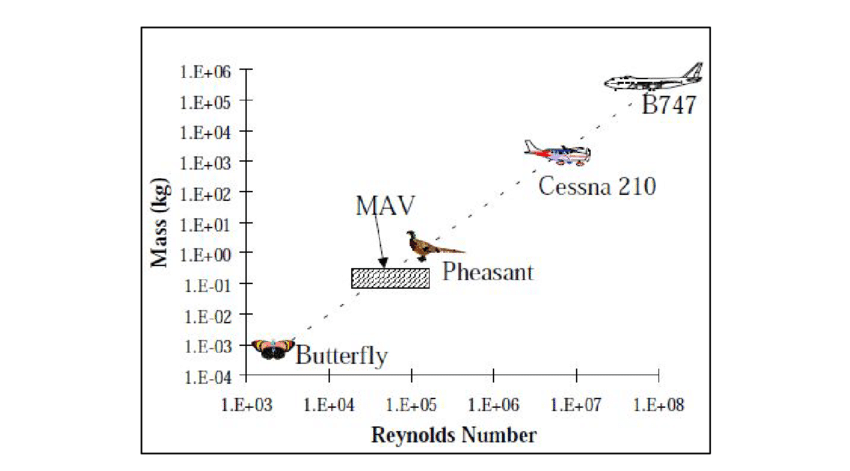
\includegraphics[width=0.8\linewidth]{images/Reynolds.png}
  \caption{Fine mesh}
  \label{fig:MAVsizes}
\end{figure}

% \\
With the increased complexity of MAV designs, there has also been increased interest in the reasearch and design of optimized MAV models \cite{Ward2017}. Current methods \todo{cite} do not produce validated, optimised and reliable designs which maximise the performance for the relevant purpose it is created for. In this area software designed to numerically optimise models based on aerodynamic properties, which are in turn mathematically determined are being used. The low Reynolds number that MAVs fly at and the influence of propeller effects on the rest of the MAV are currently unvalidated with physical wind tunnel testing. This main goal of this thesis therefore aims to fill in this gap.\\
\\
Many groups of research have \todo{cite} created software to optimize MAV's by using optimization algorthims such as generic algorthims, non-dominating sorting generic algorithms, particle swarm optimization and sequential quadratic optimisation programs. While some have accounted for low Reynolds numbers and even fewer, propeller interaction effects. None have validated these results with physical testing. These effects are expected to greatly influence the aerodynamics of MAV designs and both aspects of flight are currently unaccounted for together in physical wind tunnel testing.
\section{Background}
% Intro here

\subsection{Proliferation of MAV's in the Aerospace Landscape}
\label{subsec:ProliferationMAVs}

UAV's have existed for centuries and have been predominately used for survellience and millitary purposes \todo{cite paper}. The recent shift to the miniturization of components, systems and aerial vehicles has already influenced the military sector with several developments underway to reduce visibility of reconansance aircraft and reduce the likelihood of aircraft being detected during missions.\todo{: add examples)} What started as a small initial interest in smaller and smarter drones has resulted in exponential growth in the sector \todo{cite}. This coupled together with the growth in camera sensors and computer development, has led to the exponential growth in the capabilities of MAV seen today. Where an inital drone supported only low camera resolution with meagre flight times, today incoporates several systems such as gyrostabilisation, GPS capability with waypoint guidance, beyond the line of vision control, speeds of 70 km/h with a 30 minute flight time and a 20 megapixel camera. (DJI Phantom 4)\todo{cite Phantom}. \\

% Look at section \ref{sec:ProliferationMAVs}.

\subsection{Limitations of Current Developed MAV}
\label{subsec:Limitations}
While MAV technology is more accessible and viable to mass market than it has ever been before, there is no fully developed and validated way to optimize a MAV for a specified mission. Procedures today involve developing a CAD model of the MAV which is either then run through aerodynamic optimization software and/or tested in a wind tunnel to detemine the main characteristics of the MAV \cite{Paulson2017}. The largest drawback of which is the lack of propeller effects accounted for during wind tunnel testing. MAV model tests have been conducted with a fixed position propeller. Models are however typically tested without a free-flowing propeller, although these have been included in several aerodynamic software programs.  A lack of validation from wind tunnel testing however, means that a full understanding of the effects a propeller has on MAV's has not been conducted. Due to the small size of MAV and the large relative size of the propeller rotor disc compared to both the wing and body size it is expected that the propeller will significantly affect the stability, noise, overall endurance, performance and power consumption of a given MAV. 

\subsection{The General Micro Aerial Vechicle}
\label{subsec:GenMAV}
Today the interest, research and development of MAV's is continually increasing, however in order to focus on particular aspects or compare various designs, a "baseline" geometry is required. An example of this is the GENMAV \cite{Stewart2007}. While there are various models which have been tested to determine the main aerodyanmic properties \cite{Stewart2007}, none have completed a physical wind tunnel test while accounting for the effects of a powered propeller. Inital GENMAV aerodynamic data was determined by using the vortex-panel method \cite{Stewart2007} and did not involve wind tunnel testing. The effects of propeller induced flow has also been studied for both fixed and free-spinning propellers but currently no data is avaliable for wind tunnel tests of a powered MAV.

\subsection{Optimization Techniques and Validation}
\label{subsec:Optimization}
Many non-standard aircraft designs are evaluated using software in order to analyse aerodynamic characteristics and then optimized through a variety of typical software engineering methods such as the particle swarm method. These procedures are typically used as non-standard aircraft designs are more tedious to design and even more complex to setup and test than compared with standard aircraft designs. 

% There are many studies which have outlined methodologies for accurately determining the forces on fixed wing MAV under low Reynolds number flow streams \cite{Roberts2011} 

% \cite{Ananda2015} \cite{Roberts2011} \cite{Suhariyono2006} \cite{Zhan2012}. Propeller effects on MAV's have also been investigated


\section{Problem Statement}
\label{ProblemStatement}
MAV's are set to increase the ability to conduct a variety of missions which predominately have military or survellience objectives (todo: examples ). In the past troopers would venture on dangerous missions in order to "hopefully" gather useful information while risking their lives (todo: cite paper). Survellience was conducted initally from hot air balloons, again risking human lives. Later aircraft (mainly helicopters) would be used, costing companies large sums of money in order to survey from a birds eye view. Today drones and UAV's often conduct this work (within certain limits due to range and flight time). The next major technology jump sees the optimization and miniturization of these aircraft to produce MAV's. \\
\\
MAV's fit a niche and growing market. These aircraft are mainly used for military purposes due to the MAV's main deffering attributes; its smaller size, lower radar visibility and lower noise output.\\
\\
With MAV design becoming one of the fastest growing areas of development in the aerospace industry, there comes an increasing need to have accurate experimental data in order to validate, simulate and model the numerous MAV configurations being investigated. 

% paragraph on impact\significance of MAV
MAV's

% paragraph on current Limitations

%paragraph on lack of propeller effects


% paragraph on challenge/ main goal 
\section{Objectives}
\label{sec:Objectives}
The objectives of this thesis are as follows:

\begin{enumerate}
  \item To carry out a review of current published literature and determine areas with insufficient or no research avaliable for further development and research.
  \item To design and produce a 3D model of a generic micro aerial vechicle with interchangable empennage.
  \item To conduct wind tunnel testing of the generic micro aerial vechicle model with and without propeller effects.
  \item To analyse data of wind tunnel results and detail the affect that propeller effects have on general micro aerical vehicles.
\end{enumerate}

\section{Outline}
\label{sec:Outline}
An outline of the proposed final submission is listed below, however is subject to change.

\begin{itemize}
  \item Chapter 2: Background and literaure review of relevant topics and reasearch for this thesis
  \item Chapter 3: Proposed setup of analysis
  \item Chapter 4: Implementation
  \item Chapter 5: Results
  \item Chapter 6: Discussion
  \item Chapter 7: Conclusion
\end{itemize}



% \begin{python}[caption=Example computation]
% // Calculate the multiplication of x and y by adding x, y number of times.
% function multiply(x, y):
%   output = 0

%   for i = 0..y:
%     output = output + x

%   return output
% \end{python}


\graphicspath{{./Figs/}}

\chapter{Background} 
This section outlines the core theory and topics which are relevant for the optimization of MAV's and the effect of propeller interactions on the main wings of small MAV. MAV design is more complex than general aircraft design due to factors such as the non-linear lift distribution, low aspect ratio wings, low Reynolds number flows, structural integrity due to the small size and 


\section{Aerodynamic Parameters}
\label{sec:AerodynamicParameters}
The characteristics of an aircraft is given by a combination of the aerodynamic parameters that describe it. For MAV's this is more complex as these aircraft do not allow for the same assumptions to be made in calculations. New methods for determining the aerodyanmic parameters are currently being developed and proposed \cite{Shen2018} \cite{Roberts2011} in order to address these differences. Aerodynamic forces are cruical to the overall design of any aircraft \cite{Aero2012}. In order to determine these forces for MAV's a variety of techniques have been used such are the simple vortex lattice method \cite{Stewart2007} \cite{Hard2010}. However this method lacks the ability to predict the separetion of flow as lift is assumed to increase linearly with respect to the angle of attack \cite{Aboelezz2020}. This is not the case at low Reynolds numbers \cite{Zhang2022}. 

\cite{DeLuca2004}.
\cite{Chinwicharnam2013}

\section{Low Reynolds Number Effects }
\label{sec:LowReynolds}
Low Reynolds number compressible aerodynamics affect many different varities of aircraft. Aircraft used to survey martian terrian and MAV's are particularly influenced due to the change in atmosphere and small geometry respectively\cite{Munday2015}. This especially critical for propeller based systems as the root and tip of the mach numbers can vary significantly\cite{Munday2015}. Typically aircraft fly at high Reynolds numbers (>$10^{6}$), MAV's however generally fly between ($10^{4} and 10^{5}$) \cite{Winslow2018}.


\section{Propeller Wing Interaction}
\label{sec:Propeller Wing Interaction}
%Stability effects talked about here 

\section{MAV Optimization}
\label{sec:MAV Optimization}
Many optimization techniques exist which aim to optimize the aerodynamic design of MAV's. Algorithms such as genetic algorithms, artificial neural networks \cite{Boutemedjet2019}, 
\subsection{Wing Planform}

\subsection{Tail Planform}

\section{Non-Linear Lift Distribution}
\label{sec:Non-Linear Lift Distribution}
Early on in the study of aerodynamics, theories which were developed from the study of conventional aircraft were applied to the bodies of small flying objects and animals such as birds. Traditional aerodynamic theories provide good results and insights when steady flows move across a staionary body. They could not however explain what allows small insects and birds to fly leading to the paradox of "a bee cannot fly" \cite{bees} \cite{Roccia2016}. The issue lies in the fact that the flight of biological creatures is mainly characterized by non-linear and steady flows \cite{Roccia2016}. This non-linear lift distribution is largely caused by the low Reynolds number that these small bodies fly at and also the low aspect ratio that MAV aircraft typically have.

Wingtip vortices are particularly important and even in general aircraft lead to regulations such as spacing rules between aircraft and aerodynamic noise \cite{Qin2021}. 










\section{Stability}



\graphicspath{{./Figs/}}


\chapter{Literature Review}
This chapter contains a review of the current literature published on MAV development and the extent to which propeller effects have been researched. It explores the effects that propellers have on MAVs, current research on non-linear lift distributions, separation bubbles and propeller interactions and effects.
%  Traditional methods of aircraft design have generally focused on larger aircraft \cite{Raymer2006} \cite{Roskam1989}.

\section{Proliferation of MAV's in the Aerospace Landscape}
\label{subsec:ProliferationMAVs}
Initially introduced during World War I, UAVs were heavily criticized due to inaccuracies and unreliability when performing missions. Few saw the potential and impact they could have in changing the landscape of a battlefield \cite{thebook}. UAVs have existed for centuries, although the modern era of UAVs commonly refers to the last four decades \cite{Cook2007}. 

It was not until Operation Desert Storm (1991) and the Balkan Peninsula conflict that the development and interest in UAVs took off \cite{thebook, MacConnell2007}.  The U.S. at the time saw a total income of \$2.27 billion dollars \cite{thebook} (a 9.5\% increase from the previous year of 1996). This marked a turning point in the the development of more complex UAVs \cite{tac2022} as the U.S. Department of Defense funded UAV research for the first time in 1996 \cite{keennon2003}. The recent shift to the miniaturisation of components, systems and aerial vehicles has already influenced the military sector \cite{Aleksander2018, Mil2022}, with several developments underway to reduce the visibility of reconnaissance aircraft and reduce the likelihood of aircraft being detected during missions \cite{Greenwood2019, Saytov2022}.  The most famous military MAV arguably being the Honeywell RQ-16 T-Hawk \cite{Agbeyangi2016}  which was mainly used by the U.S. forces in Iraq to search for roadside bombs \cite{Crivoi2022}. The success of which (largely due to its hovering feature) led the U.S. Navy to order a further 372 MAVs \cite{design2022}.

What started as a small initial interest in smaller and smarter drones has resulted in exponential growth in the sector \cite{NONAMI2007, Wang2019}. Technology improvements have led to the exponential growth in the capabilities of MAV seen today \cite{Yin2020, Jackson2016}. Where an initial drone supported only low camera resolution with meagre flight times, today incorporates several systems such as gyro stabilisation, GPS capability with way-point guidance, beyond the line of vision control, speeds of 70 km/h with a 30 minute flight time, and a 20-megapixel camera (DJI Phantom 4) \cite{Peppa2019}. 




% Look at section \ref{sec:ProliferationMAVs}.

\section{Limitations of MAV Design Techniques}
\label{subsec:Limitations}
While MAV technology is more accessible and viable to the mass market than it has ever been before \cite{Jackson2016}, there is no fully developed and validated way to optimize a MAV for a specified mission \cite{Bronz2009, HASSANALIAN2019}. Today, procedures involve developing a CAD model of the MAV or using software based on aerodynamics. This model is either then run through aerodynamic optimization software and/or tested in a wind tunnel to determine the main characteristics of the MAV \cite{Paulson2017}. The largest drawback of which is the lack of propeller effects accounted for, which are known to have a large effect on aerodynamics and stability \cite{Harikumar2021, Chinwicharnam2013}. MAV model tests have been conducted with a fixed position propeller \cite{Shams2020b, Durai2014}. Models are, however, typically tested without a spinning propeller, although these have been included in several aerodynamic software programs and specific tests \cite{Aboelezz2020}. 

However, a lack of validation from wind tunnel testing means that a full understanding of the effects a propeller has on MAVs has not been achieved. MAVs are small relative to the size of the propellers used. Hence, the propeller will significantly affect the stability, noise, overall endurance, performance and power consumption of a given MAV \cite{Shams2020, Chen2022}. 



\section{Low Reynolds Number Effects }\label{sec:Reynolds2}

% EXPLAIN HERE - what is RE
\label{sec:LowReynolds}
Due to the small size and Reynolds numbers at which MAVs operate (typically around Re=$10^5$ \cite{Huq2009} \cite{Winslow2018}), insects and other small animals are often studied to understand the flight dynamics which occur for small flying bodies \cite{Liu2009}. The Reynolds region in which MAVs typically fly is shown in Figure \ref{fig:MAVsizes}.

\begin{figure}[H]
% \hspace*{-1.3in}
  \centering
  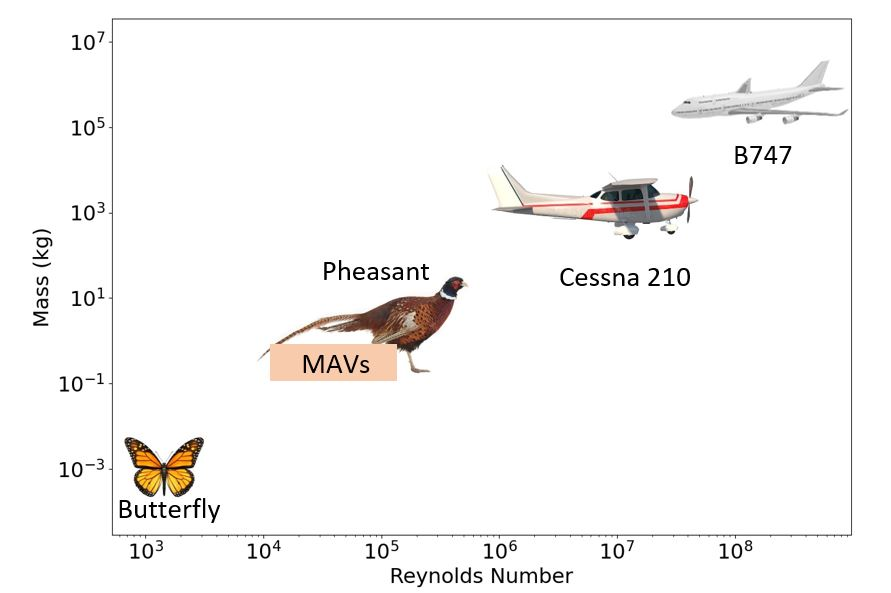
\includegraphics[width=\linewidth]{03_LiteratureReview/Figs/Reynolds.JPG}
  \caption{MAV speed with Reynolds number region in respect to flying bodies. Figure is adapted \cite{reynoldsFigure}. Image sources: \cite{butterfly, pheasant, cess, b474} }
  \label{fig:MAVsizes}
\end{figure}

 Null used wind tunnel tests to show that propellers on wings during low Reynolds flight increased the performance of the wing at high angles of attack \cite{Null2005}. Ananda also visualised this effect as shown in Figure \ref{fig:bladeslow}, however this is without the propeller being mounted on the wing directly.  

\begin{figure}[H]
% \hspace*{-1.3in}
  \centering
  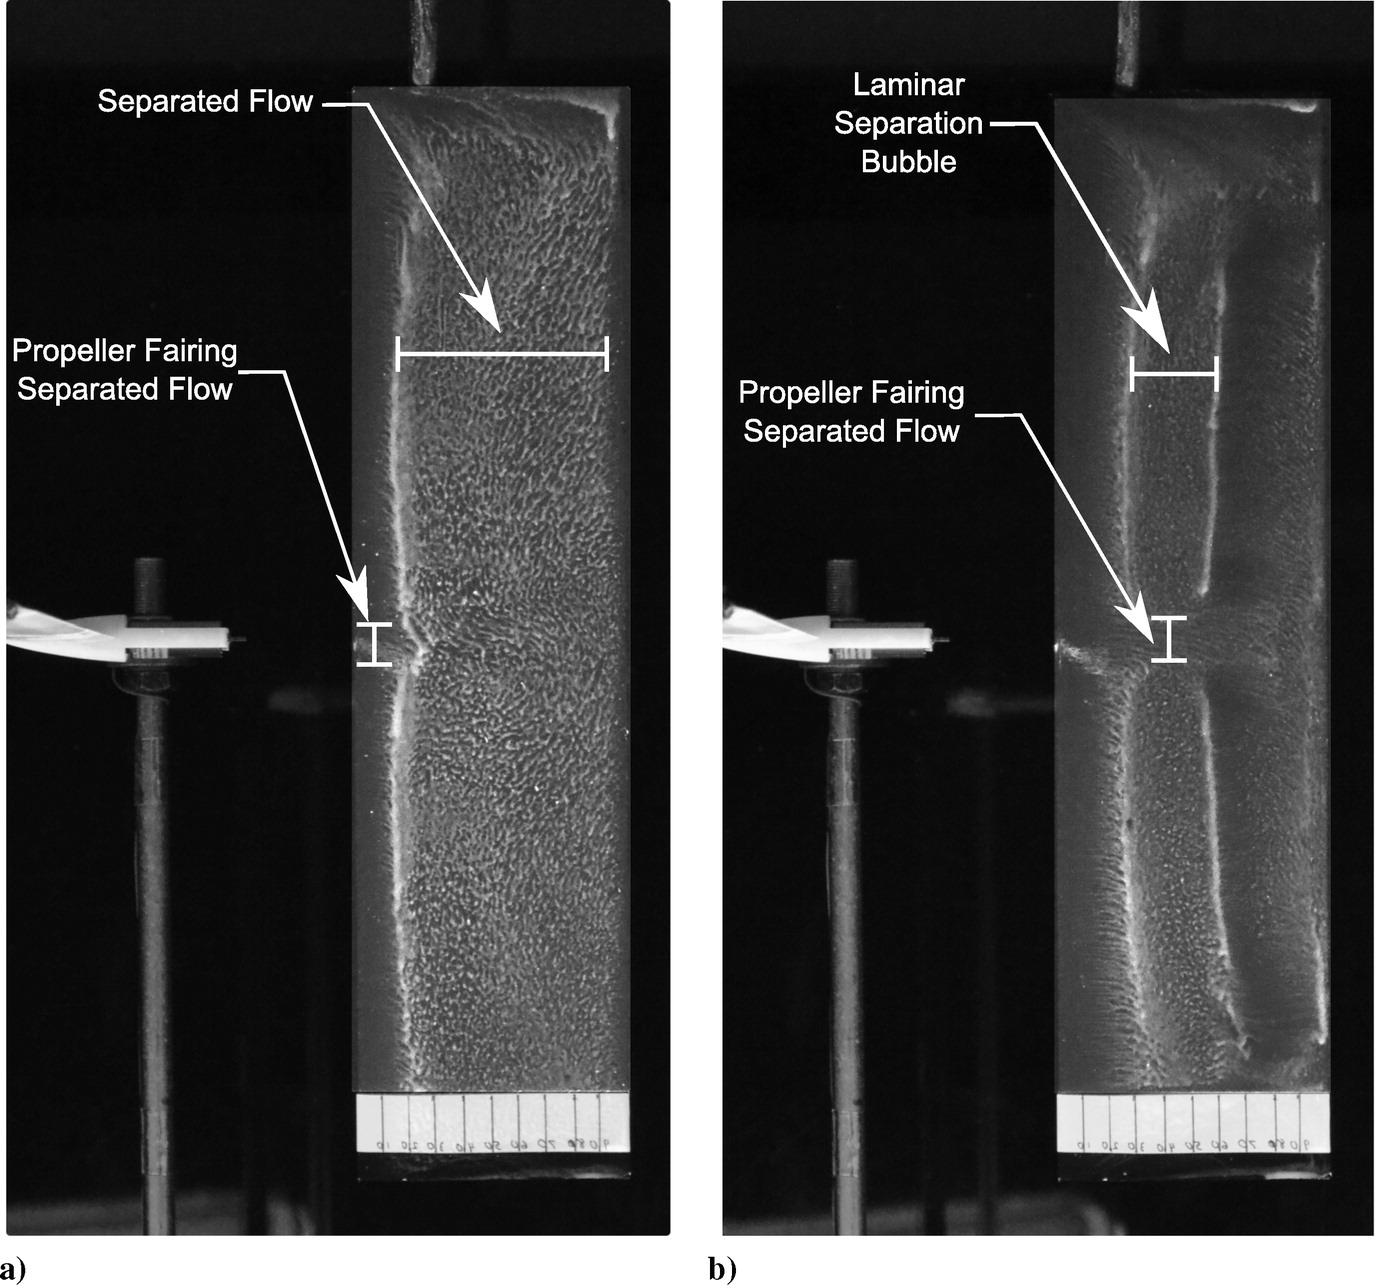
\includegraphics[width=0.8\linewidth]{03_LiteratureReview/Figs/blades.jpeg}
  \caption{Flow characteristics across the propeller when the propeller is turned off (a) and when the propeller is turned on (b) \cite{Ananda2018}}
  \label{fig:bladeslow}
\end{figure}



% \begin{figure}[H]
% \hspace*{-1.3in}
%   \centering
%   \includegraphics[width=\linewidth]{03_LiteratureReview/Figs/285202324_1193411864727797_5746060971373574289_n.png}
%   \caption{MAV speed with Reynolds number region in respect to flying bodies \cite{reynoldsFigure}}
%   \label{fig:MAVsizes}
% \end{figure}

Low Reynolds number compressible aerodynamics are particularly important for small aircraft. Aircraft used to survey martian terrain and MAVs are mainly influenced due to the change in atmosphere and small geometry respectively \cite{Munday2015}. Low Reynolds number effects are critical for propeller based MAV systems. As the root and tip of a propeller can differ significantly in Mach number \cite{Munday2015}. As MAVs have small ARs due to their smaller size and non-conventional structures, low AR wings at low Reynolds numbers have recently, in particular, been studied \cite{Bhat2019} \cite{Torres2012}. Cosyn showed that the flow over these is characterised by complex 3D phenomena such as wing-tip vortices, laminar to turbulent transitions, and flow separation, and re-attachment \cite{Cosyn2012}.

Airfoils in particular have been investigated due the importance of their use in aircraft. At low Reynolds numbers (10,000 < Re < 50,000) the flow remains laminar when the airfoil is aligned with the incoming flow. Pressure gradients created due to a larger angle of attack or high camber (airfoil thickness) create turbulent flow following separation. This is also shown in Figure \ref{fig:Re3}. Early research by Mueller showed that the maximum lift coefficient is typically 0.5 for airfoils before stalling at low Reynolds numbers \cite{Mueller1985}. \\
At Reynolds numbers from 50,000 to 100,000 the separation bubble and turbulent layer thickness increase in size \cite{Winslow2018}. The separated shear layer will eventually gain enough momentum from the free-stream in order to reattached to the airfoil as shown in Figure \ref{fig:Re3}. The separation bubble is also known as a laminar separation bubble (LSB). Mueller found that airfoil choice in this region was critical to the aerodynamic performance. Airfoils with large camber (thickness) produce large pressure gradients causing separating which leds to the formation of LSBs on the upper surface of the wing \cite{Mueller1985}. As Reynolds numbers increases the separation and attachment move towards the leading edge \cite{Winslow2018}. The turbulent layer thickess reduces and the airfoil performance improves. The turbulent layer thickness varies between airfoils and LSBs can still form up until around a Reynolds number of 200,000. This is notable as most MAVs operate around the 50,000 to 200,000 Reynolds number range \cite{Cosyn2006}. At Reynolds numbers greater than 500,000 the separation point generally lies on the leading edge. The performance of airfoils increases due to the reduced turbulent layer \cite{Winslow2018}. %Separation however can occur at high angles of attack. Turbulent boundary layer initially separates from the tailing edge but this separation will move towards the leading edge as the angle of attack increases. This can lead to stall of the entire airfoil \cite{Winslow2018}. 

\begin{figure}[H]
    \centering
    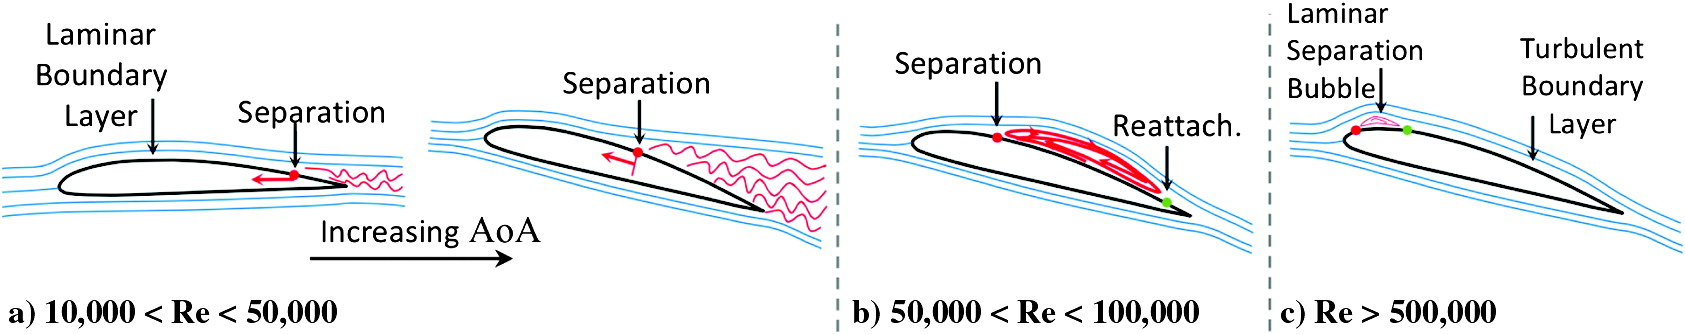
\includegraphics[width = \linewidth]{02_Background/Figs/airfoil.jpeg}
   \caption{Flow separation position change with Reynolds number \cite{Winslow2018}}
    \label{fig:Re3}
\end{figure}

\subsection{Laminar Separation Bubbles and Vortices}
Flow separation and re-attachment create separation bubbles over wings and account for the most drag over the surface of wings at these low Reynolds numbers \cite{ravi}. LSBs typically occur at Reynolds number below 200,000. Perot showed how in the presence of adverse pressure gradients, airflow separates from the wing \cite{Perot1999}. This was further validated by Mohamed \cite{Mohamed2014}. Mohamed investigated these LSBs and showed that they can deteriorate a MAVs stability as the drag induced by these bubbles leads to a low-pressure region over the bubbles, causing severe perturbations of motion \cite{Mohamed2014}. Marxen found these bubbles are typically stable, as no transfer of energy occurs between the flow circulating inside the bubble and the laminar flow, which passes over the top \cite{Marxen2010}. Detailed anatomy of how LSBs affect flow over a typical airfoil shape is shown in Figure \ref{fig:Laminar}.

% CITE ISSUETODO

\begin{figure}[H]
% \hspace*{-1.3in}
  \centering
   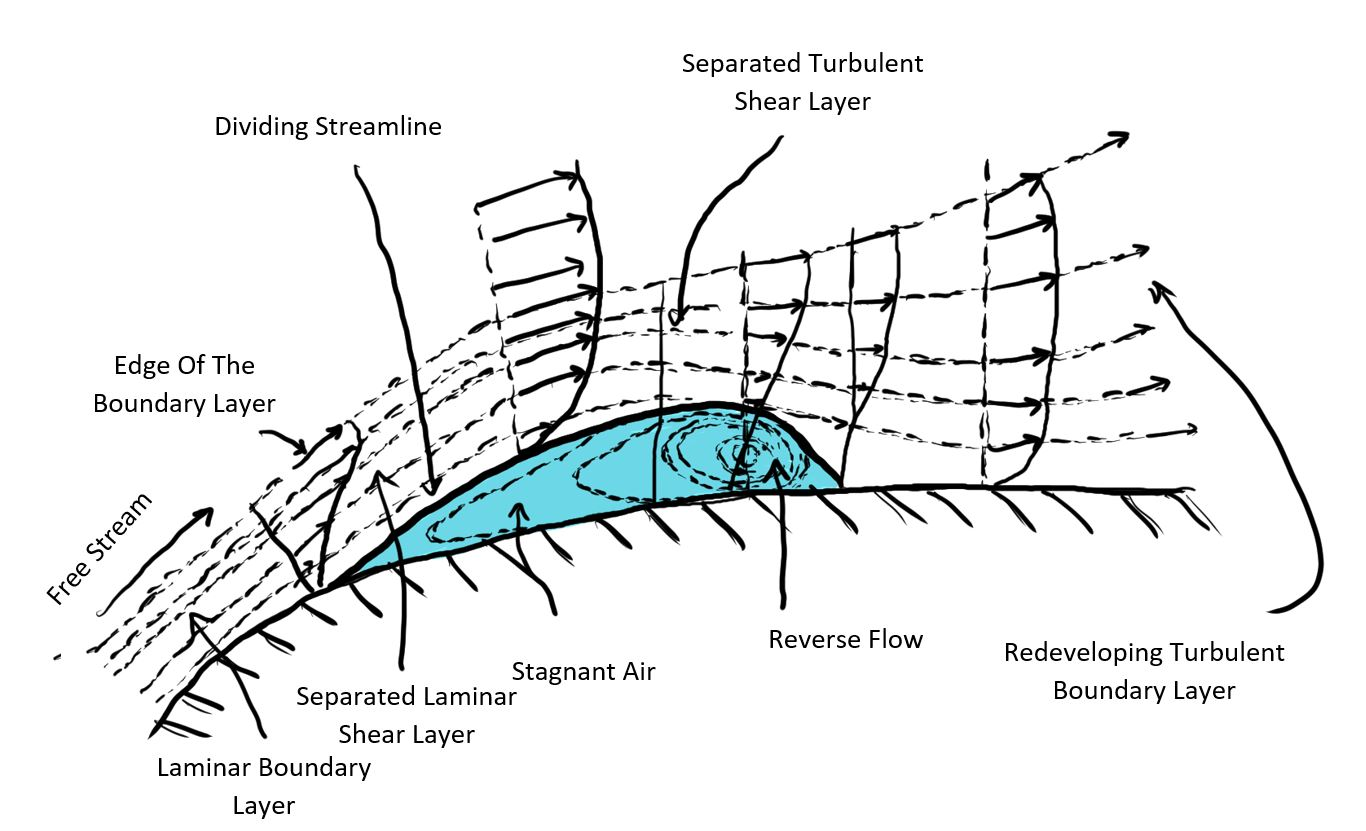
\includegraphics[width=\linewidth]{03_LiteratureReview/Figs/LSB.jpg}
  \caption{Anatomy of laminar separation bubbles. Figure adapted from Mohamed \cite{Mohamed2014}}
  \label{fig:Laminar}
\end{figure}

Crimi then investigated the implications of this separation when varying the angle of attack. Crimi determined that the angle of attack of an airfoil affects the placement of LSBs. When the angle of attack suddenly increases (e.g. during a gust), a separation of the shear layer is also seen close to the leading edge \cite{Crimi1976}. Mohamed explains this as the shear layer transitioning earlier due to this disturbance  \cite{Mohamed2014}. Additionally, LSBs and vortices also significantly affect the coefficient of lift ($C_L$) of an airfoil. $C_L$ is affected to a greater extent in smooth flow conditions as more suction is experienced inside an LSB with a smooth surface.


% \begin{figure}[H]
%      \centering
%      \begin{subfigure}[b]{\textwidth}
%          \centering
%          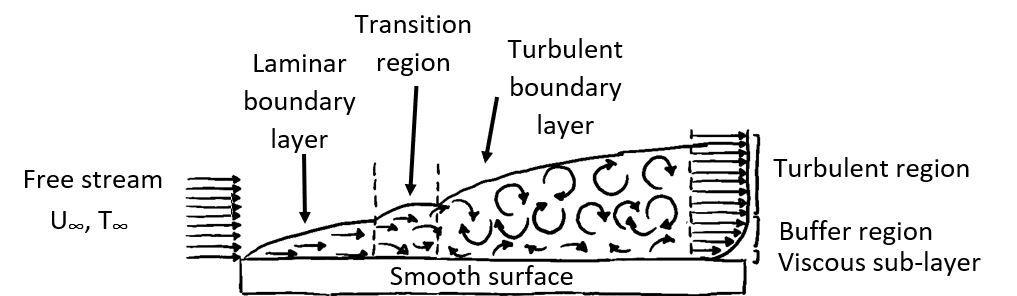
\includegraphics[width=\textwidth]{02_Background/Figs/smooth.JPG}
%          \caption{Smooth surface}
%          \label{fig:Pressoo2a}
%      \end{subfigure}
%      \hfill
%      \begin{subfigure}[b]{\textwidth}
%          \centering
%          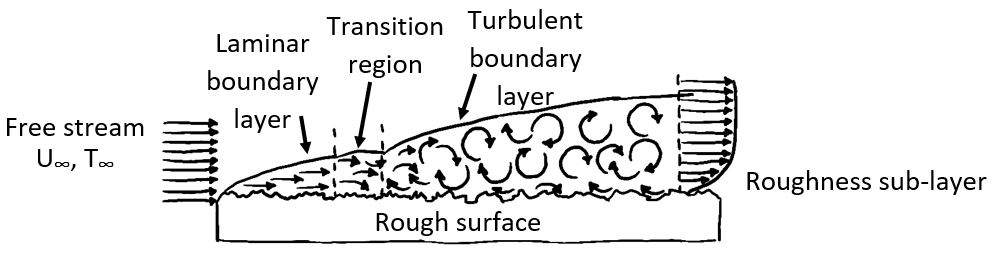
\includegraphics[width=\textwidth]{02_Background/Figs/rought.JPG}
%          \caption{Rough surface}
%          \label{fig:Pressoo2b}
%      \end{subfigure}
%      \hfill
%          \caption{a) Laminar flow to turbulence without surface roughness. b) Smaller transition region and turbulent boundary layer length with a rough surface. Figure is adapted \cite{Choi2006}.}
%   \label{fig:compare}
% \end{figure}


Mohammed found this larger suction seen on smooth surfaces, induces pitching and rolling moments \cite{Mohamed2014}. In the stall region angle of attack, turbulent flow results in a higher lift. The opposite is true for smooth flow. Turbulence could therefore increase the characteristic airfoil performance at low Reynolds numbers \cite{Mohamed2014}. These characteristics are also shown in Figure \ref{fig:flow}.


\begin{figure}[H]
     \centering
     \begin{subfigure}[b]{0.45\textwidth}
         \centering
         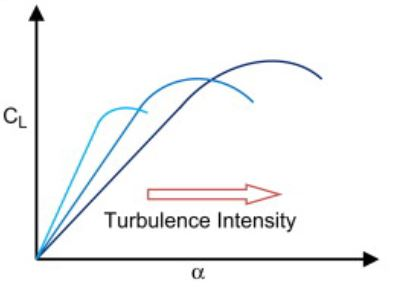
\includegraphics[width=\textwidth]{03_LiteratureReview/Figs/acondition.JPG}
         \caption{Turbulence Intensity with lift curve}
         \label{fig:P2a}
     \end{subfigure}
     \hfill
     \begin{subfigure}[b]{0.45\textwidth}
         \centering
         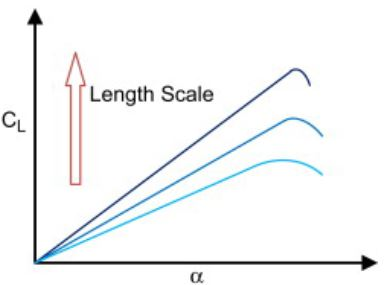
\includegraphics[width=\textwidth]{03_LiteratureReview/Figs/bcondition.JPG}
         \caption{Length scale with lift curve}
         \label{fig:P2b}
     \end{subfigure}
     \hfill
          \caption{Airfoil aerodynamic performance variation with increasing: (a) turbulence intensity (b) length scale \cite{Mohamed2014}}
        \label{fig:flow}
\end{figure}





Investigations using materials with varying roughness have also been used to induce this transition to turbulent flow. Choi investigated this transition with some results shown in Figure \ref{fig:rough}. These show that the LSBs are reduced in the flow over airfoils when moving over a rough surface.

% ISSUE
\begin{figure}[H]
     \centering
     \begin{subfigure}[b]{0.45\textwidth}
         \centering
         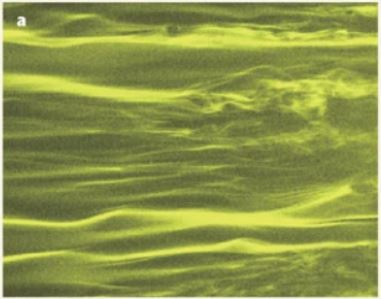
\includegraphics[width=\textwidth]{03_LiteratureReview/Figs/a2.JPG}
         \caption{Smooth surface}
         \label{fig:Ps2a}
     \end{subfigure}
     \hfill
     \begin{subfigure}[b]{0.45\textwidth}
         \centering
         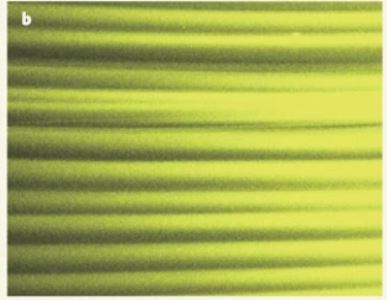
\includegraphics[width=\textwidth]{03_LiteratureReview/Figs/b2.JPG}
         \caption{Rough surface}
         \label{fig:Ps2b}
     \end{subfigure}
     \hfill
           \caption{Flow patterns shown by smoke. Laminar flow to turbulence without surface roughness (a). Laminar flow for with a rough surface (b).  \cite{Choi2006}}
  \label{fig:rough}
\end{figure}







% Modelling LSBs and vortices in software is a difficult challenge and software such as Xfoil are unable to account for concepts such as the 'bursting of laminar bubble' which is a concept in which the free-stream airflow does not reattach to the airfoil. 

\subsection{Non-Linear Lift Distribution}


\label{sec:Non-Linear Lift Distribution}
Early on in the study of aerodynamics, theories developed from the study of conventional aircraft were applied to the bodies of small flying objects and animals such as birds. Traditional aerodynamic theories provide good results and insights when steady flows move across a stationary body. As mentioned by Roccia, they could not however, explain what allows small insects and birds to fly, leading to the paradox of "a bee cannot fly" \cite{bees} \cite{Roccia2016}. Roccia determined that the issue lies in the fact that non-linear and steady flows mainly characterize the flight of biological creatures \cite{Roccia2016}. This non-linear lift distribution is primarily caused by the low Reynolds number that these small bodies fly at and the low AR that MAV aircraft typically have (AR < 3).

 Early experimental work conducted by Winter showed that wings with small ARs can be described with a bound vortex flow and a wing-tip flow, which is also known today as vortices \cite{H1936}. Wingtip vortices are particularly important, and even in general aircraft, lead to regulations such as spacing rules between aircraft and aerodynamic noise \cite{Qin2021}. At the wingtips the pressure difference between the upper and lower surface cause a swirling vortex when in a free stream flow. This phenomenon is also shown in Figure \ref{fig:vortex}. Cosyn and Vierendeels showed that this creates a low pressure cell at the wing tip which deforms the lift distribution in this region \cite{Cosyn2006}. 
 
 \begin{figure}[H]
% \hspace*{-1.3in}
  \centering
  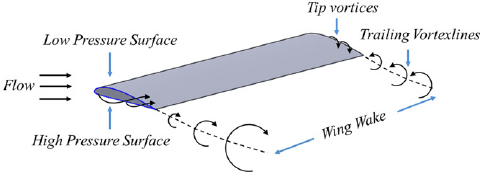
\includegraphics[width=\linewidth]{03_LiteratureReview/Figs/Development-of-wingtip-vortices-over-a-wing-section.png}
  \caption{ Development of wingtip vortices over a wing section 
 \cite{Kumar2015}}
  \label{fig:vortex}
\end{figure}

 Zimmerman showed that the wing-tip geometry influences the aerodynamic performance for low AR wings \cite{Zimmerman1936}. Zimmerman also concluded that in order to produce the same coefficient of lift for lower AR wings, a higher angle of attack is required \cite{Zimmerman1936}. Low AR wings are also more susceptible to instability caused by disturbances \cite{DeVoria2017}. Watkins showed that a sideslip is easily induced by a slight wind gust for low AR aircraft \cite{Watkins2012}. Shields investigated the inherent stability modes of low AR wings, determining that low AR wings have near-zero roll damping \cite{Shields2015}. This means that roll moments created by flow asymmetries have a significant impact on low AR aircraft \cite{Shields2015}.
 
 Mueller and DeLaurier found that for low AR aircraft, the center of lift was also sensitive to the angle of attack \cite{Mueller2003}. This is due to the wingtip vortices increasing with angle of attack. Therefore the non-linear aerodynamics dominate more at higher angle of attack, Pelletier also determined that these effects are more pronounced for low AR aircraft \cite{Pelletier2012}. 


\section{Propeller Wing Interaction}




Propellers are commonly mounted on wings and significantly alter the flow seen over airfoils. Prandtl first studied the propeller-wing interaction at the start of the last century. The results concluded that two main effects impact the wing and flow behaviour. The first is due to the swirling of the propeller, which creates an ever-varying velocity. The second is due to an increase in inflow velocity \cite{Pant}. Mounting propellers on the tips of the wing has also been shown to have benefits to performance compared with other wing positions \cite{Miranda1986}. Miranda found that substantial performance improvements can be achieved by properly mounting propellers on the wingtips of wings \cite{Miranda1986}, this was also further validated by Sinnige \cite{Sinnige2019} and other teams \cite{Veldhuis2000} \cite{review}. 

Numerical analysis by Rizk using the Vortex Lattice Method has also validated these observations \cite{Rizk2012}. Veldhuis found that propellers have a higher axial velocity at the blade tip than where it is joined at a hub \cite{Veldhuis2000}. Ferraro also determined that the slipstream created by the propeller can be split into the axial, and tangential velocity components \cite{Ferraro2014}. The tangential velocity component accounts for the dynamic pressure across the wing \cite{Ferraro2014}. The swirl is anti-symmetrical and changes the incoming flow that the wing sees. This is also shown in Figure \ref{fig:2a} \cite{Ferraro2014}. The axial velocity affects the dynamic pressure on the wing. The axial velocity is considered to be symmetric when the propeller flow is uniform and undisturbed, as shown in Figure \ref{fig:2b} \cite{Ferraro2014}.


\begin{figure}[H]
     \centering
     \begin{subfigure}[b]{0.4\textwidth}
         \centering
         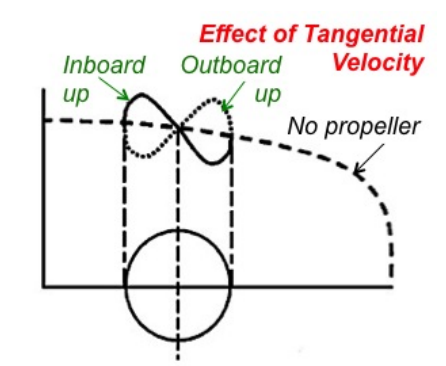
\includegraphics[width=\textwidth]{03_LiteratureReview/Figs/tanget.png}
         \caption{Tangential propeller effects}
         \label{fig:2a}
     \end{subfigure}
     \hfill
     \begin{subfigure}[b]{0.4\textwidth}
         \centering
         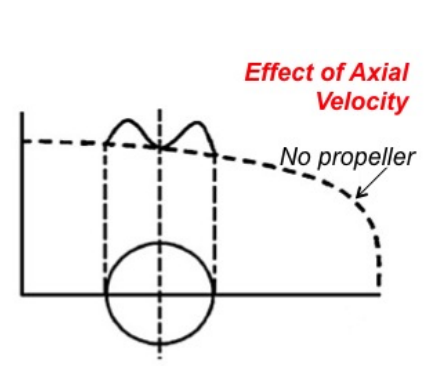
\includegraphics[width=\textwidth]{03_LiteratureReview/Figs/axial.png}
         \caption{Axial propeller effects}
         \label{fig:2b}
     \end{subfigure}
     \hfill
        \caption{Tangential and Axial velocity effects \cite{Ferraro2014}}
        \label{fig:prop}
\end{figure}


\begin{figure}[H]
% \hspace*{-1.3in}
  \centering
  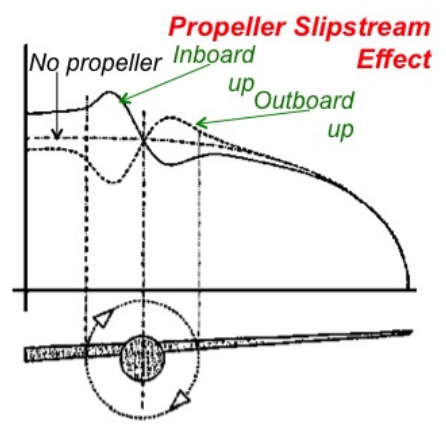
\includegraphics[width=0.4\linewidth]{03_LiteratureReview/Figs/slipstream.png}
  \caption{ Propeller slipstream effects on a finite wing \cite{Ferraro2014}}
  \label{fig:overallProp}
\end{figure}

As the dynamic pressure increases, a gain in lift coefficient is seen as shown in Figure \ref{fig:propanswer}. This increase in lift coefficent is also partially due to the lack of separation seen when increasing the revolutions per minute (RPM) of the propeller. Shams shows that this leads to a forward shift in the aerodynamic center of the aircraft \cite{Shams2020} \cite{Shams2020b}.


\begin{figure}[H]
% \hspace*{-1.3in}
  \centering
  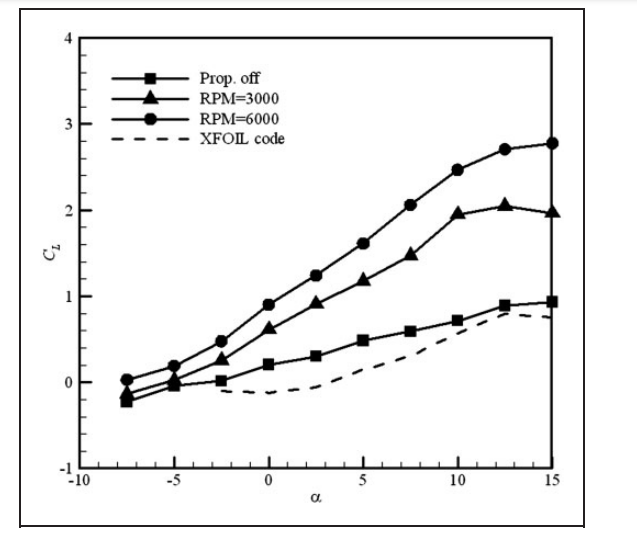
\includegraphics[width=0.8\linewidth]{03_LiteratureReview/Figs/Cl.png}
  \caption{ Effect of propeller slipstream on the lift coefficient
curve with angle of attack (Re =0.3 x $10^5$
) \cite{Aminaei2019}.}
  \label{fig:propanswer}
\end{figure}


The slipstream effect is shown in Figure \ref{fig:peoptoyou}. The inboard wing sees a higher angle of attack, and hence an up-wash effect is seen (y/b $>$ 0). Aminaei found that in the propeller down-wash region (y/b $<$ 0) a delay is experienced in the flow transition than when compared with the up-wash region \cite{Aminaei2019}. This is due to the reduced local angle of attack on the wing, which moves the transition region towards the trailing edge. These effects can also affect the flow stream beyond the propeller and lead to non-linear lift distributions further from the propeller as well. 
 
\begin{figure}[H]
% \hspace*{-1.3in}
  \centering
  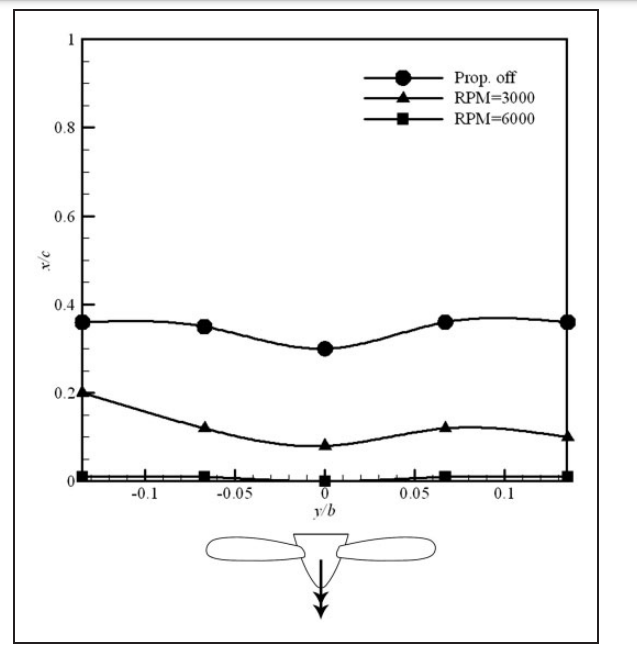
\includegraphics[width=0.8\linewidth]{03_LiteratureReview/Figs/propeller effects.png}
  \caption{Propeller slipstream effect with span-wise location for airflow transition over the wing upper surface, $\alpha = 2.5 ^\circ$ \cite{Aminaei2019}.}
  \label{fig:peoptoyou}
\end{figure}

    Prantl was one of the first to investigate the influence of propellers on wings \cite{Prandtl1931} and Franke and Weinig one of the first to investigate the rotational velocity's effects on the lift distribution across the wing \cite{Franke1939}. Framk and Weinig showed that the circulation distribution in regards to the slipstream can be predicted and used the lifting line theory in order to prove this \cite{Franke1939}. Jameson went on to develop simple equations to quantify the lift and drag of wings in jet slipstreams \cite{Jameson1970}. Ellis devloped programs to run multiple lifting line approximations in order to quanitfy the circulation pattern, when propeller effects are being accounted for \cite{Ellis1971}. These approximations however, were all too rudimentary and could not be used to predict the flow characteristics over wings. Several models and equations to represent these effects have been created. Veldhuis concluded that the propeller effects can only be described completely when using the Full Interaction Mode (FIM) \cite{Veldhuis2004}. 

% Up to Veldhuis

Veldhuis also determined that there are four main regions of influence which the propeller has. These proposed sections are not independent of each other but rather act as a smooth transition from one to the other \cite{Veldhuis2004}. As shown in Figure \ref{fig:propfour} the local blade angle of attack increases where the blade move down (P-II in Figure \ref{fig:propfour}) and decreases where the blade moves up (P-IV in Figure \ref{fig:propfour}). The induced angle of attack is visualised in Figure \ref{fig:propangles}. The effect of the propeller to induce this change in effective angle of attack is most greatly seen when the propeller is parallel to the wing span \cite{Veldhuis2004}.

\begin{figure}[H]
% \hspace*{-1.3in}
  \centering
  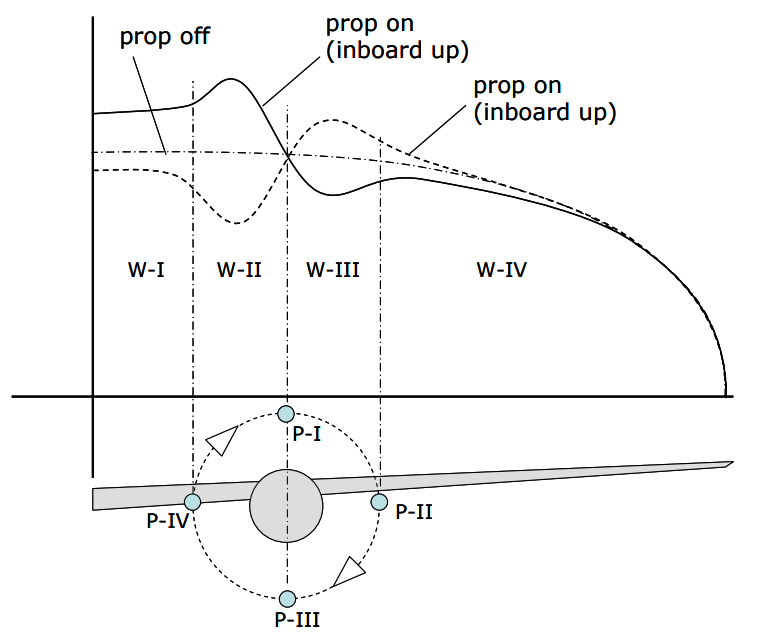
\includegraphics[width=0.8\linewidth]{03_LiteratureReview/Figs/four.png}
  \caption{Influence areas related to propeller-wing interaction based on the loading distributions \cite{Veldhuis2004}}
  \label{fig:propfour}
\end{figure}

\begin{figure}[H]
% \hspace*{-1.3in}
  \centering
  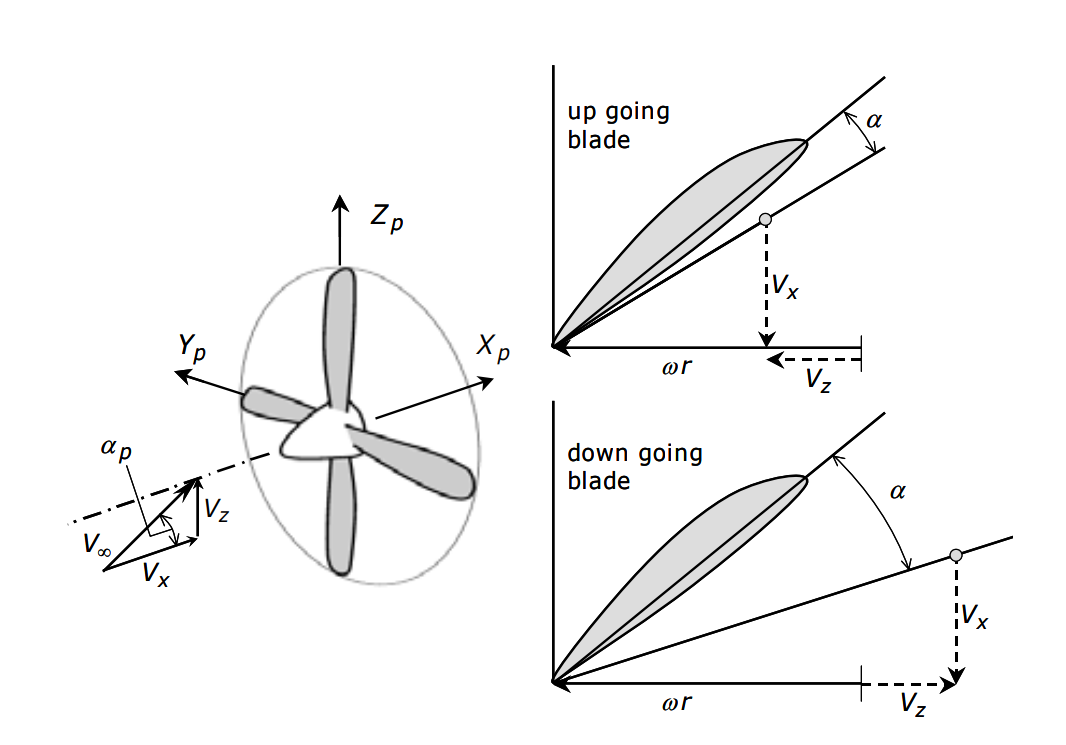
\includegraphics[width=0.8\linewidth]{03_LiteratureReview/Figs/anlges.png}
  \caption{Blade angle of attack variation due to propeller pitch angle \cite{Veldhuis2004}}
  \label{fig:propangles}
\end{figure}

Veldhuis also found that the extent of the swirl relaxation is dependent on the propellers position, free stream conditions and the overall wing loading \cite{Veldhuis2004}. A more recent study by Veldhuis simulated these effects through the use of CFD \cite{Veldhuis2016}. Ananda also concludes that for the tractor configuration, in a low speed wind tunnel, the flow transistions to turbulent flow earlier. This reduces the drag and increases the lift to drag ratio. These benefits were not seen when analysing the pusher configuration. 












%Tractor/pusheer mounted





% \cite{Harikumar2021} Shams investigated the left turning tendencies of right-handed propellers \cite{Shams2020} \cite{Chen2022} \cite{Aminaei2018} \cite{Null2005} \cite{Parga2007}  \cite{Jana2020}. 

\subsection{Stability Effects}
As propellers have been shown to have a strong influence on the lift distribution across wings, the overall lateral and longitudinal stability will be affected. Shams has showed that increasing the propeller diameter and RPM increase the moment produced creating a larger pitching moment on the aircraft \cite{Shams2020}. Tractor configurations have also been investigated by Shams. The tractor configuration creates an increase in the rolling and yaw moments acting on the aircraft \cite{Shams2020}. Propellers do also produce a torque effect, further destabilizing the aircraft by creating a asymmetric roll. 

\subsection{Aerodynamic Parameters}
\label{sec:AerodynamicParameters}
The characteristics of an aircraft are given by a combination of the aerodynamic parameters that describe it. For MAV, this is more complex as these aircraft do not allow for the same assumptions to be made in calculations. New methods such as those developed by Shen, for determining the aerodynamic parameters are currently being developed, and proposed in order to address these differences \cite{Shen2018, Roberts2011}. Aerodynamic forces are crucial to the overall design of any aircraft \cite{Aero2012}. In order to determine these forces for MAVs, a variety of techniques have been used, such as the Athena Vortex Lattice Method used by Stewart and Hrad \cite{Stewart2007, Hrad2010}. However, this method cannot predict the separation of flow as the lift is assumed to increase linearly with the angle of attack.  This is not the case at low Reynolds numbers \cite{Zhang2022}. Aboelezz outlines a process in which a fixed-wing MAV can be designed, whereby he uses physical wind tunnel testing in order to evaluate the MAVs actual flight performance \cite{Aboelezz2020}. Bollay and Belotserkovskii have both proposed modified versions of Prandtl's lifting line theory \cite{Bollay1939, Belotserkovskii1968}, though validations with experimental data are limited in scope and do not validate propeller-wing interactions.

\subsection{The General Micro Aerial Vehicle}
\label{subsec:GenMAV}
Today the interest, research and development of MAVs are continually increasing. However, in order to focus on particular aspects or compare various designs, a "baseline" geometry is required. An example of this is the GENMAV developed by Stewart \cite{Stewart2007} shown in Figure \ref{fig:genmav2}.

\begin{figure}[H]
    \centering
    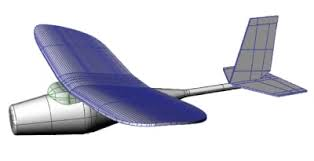
\includegraphics[width=0.8\linewidth]{04_Progress/Figs/genMav.jpeg}
    \caption{GenMAV Model \cite{Stewart2007}}
    \label{fig:genmav2}
\end{figure}

While there are various models which have been tested to determine the main aerodynamic properties \cite{Stewart2007} \cite{Aboelezz2020}, none have completed a physical wind tunnel test while accounting for the effects of a powered propeller. Initial GENMAV aerodynamic data was determined by using the vortex-panel method by Stewart \cite{Stewart2007}, and did not involve wind tunnel testing. The effects of propeller induced flow have also been studied for both fixed and free-spinning propellers, but currently, no data is available for wind tunnel tests of a powered propeller MAV.

\subsection{Optimization Techniques and Validation}
\label{subsec:Optimization}
Many non-standard aircraft designs are evaluated using software to analyse aerodynamic characteristics and then optimised through a variety of typical software engineering methods such as the particle swarm method used by Gomez to optimize the algorithm for the attitude and altitude, and Boutemedjet who used this to optimize the wing planform parameters of a MAV \cite{Gomez2020, Boutemedjet2019}. These procedures are used, as non-standard aircraft designs are more tedious to design and even more complex to set up and test than standard aircraft designs. The unique constraints that MAVs have and how they led to poor attitude control are shown in Figure \ref{fig:MAVconstrain}.

\begin{figure}[H]
% \hspace*{-1.3in}
  \centering
   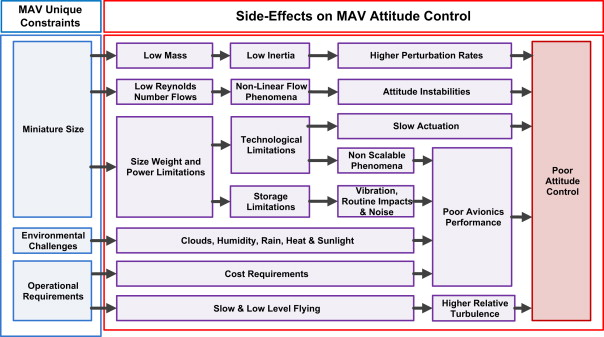
\includegraphics[width=\linewidth]{03_LiteratureReview/Figs/fowchart.jpg}
  \caption{Unique constraints of MAVs \cite{Mohamed2014}}
  \label{fig:MAVconstrain}
\end{figure}

Mohamed found that the physical size, environment and flight regime have strong effects on a MAVs ability to fly and carry payloads \cite{Mohamed2014}. Many groups of researchers have created software to optimize MAVs by using optimization algorithms such as genetic algorithms, non-dominating sorting generic algorithms, particle swarm optimization and sequential quadratic optimization programs. While some have accounted for low speed flight \cite{Vijayanandh2019, Bronz2009, HASSANALIAN2019}, no optimization techniques accounting for propeller-interaction effects currently exist. Many investigations into propeller effects show the propeller has significant effects on wing aerodynamics, both in regards to performance and also stability \cite{Parga2007, Jana2020}. None have been used with the results of spinning propellers in physical wind tunnel testing. Therefore these software models are currently invalid when also accounting for propeller-wing effects.

%  \cite{Harikumar2021} \cite{Shams2020b} \cite{Chen2022} \cite{Aminaei2018} \cite{Null2005}


\graphicspath{{./Figs/}}

\chapter{Theory and Methodology}
This chapter outlines the theory and Methodology used create, test and collect the data required for the wing-propeller interaction analysis. 

\section{Material Choice}
In order to readily edit and modify the model to be tested 3D printing was used to print the final developed model. 3D printing has become increasingly common when developing models to be testing in wind tunnels. Polyatic acid (PLA) filament was used to print the main body of the model as this is the most widely used and avaliable filament for 3D printing purposes. It has a reasonably low melting point of $\approx$ 150 $^{\circ}$. good layer adhesion and. It can also be extruded in a variety of ways in order to develop different textures on the surface of the 3D model. This is partiularly significant for MAVs as the surface of aircraft are typically smooth in order to reduce viscous drag effects. 3D printed models often have ridges between layers which have been printed. However \todo{interrogate Ben}


\section{FreeCAD}
FreeCAD is a 3D parametric modeler and was used with provided python scripts to produce fuselage, wing and tail shapes when given input parameters to define the shape and geometry. Various model shapes were produced with the aim of making the model 3D printable in order to allow for ease of manufacturing and testing. Several design constraints had to be considered when developing the model due to the structural strength of the PLA used for 3D-printing and the limitations . the wings and tail could not be 
\todo{finish + add photo}

The model was also fitted to mount into the 3x4 wind tunnel for testing as shown in Figure \todo{add figure here}

\section{VAP 3.5}
VAP 3.5 is a open-source software which uses the High-Order Free Wake (HOFW) \todo{abb} method in order to determine the aerodynamic performace of MAV designs. \\

The HOFW method


\section{XFOIL}
XFOIL is another open source free to use software which has been developed by Harold Youngren and Mark Drela. The software is used to analyse 2D airfoils for their aerodynamic characteristics. XFOIL was used to produce aerofoil data which accounted for viscous effects. It is essential that the software account for the viscous effects as this has an essential role in the flow characteristics accross the surface of an aircraft wing. This is especially true at low Reynolds numbers where the  \todo{finsiht this}. XFOIL accounts for the viscous effects by using the wake momentum thickness to determine the skin friction produced as fluid passes over the surface of the airfoil as given by Equation \ref{eqn:XFOIL}. 


\begin{equation}
    \theta = \int_{0}^{\infty} \frac{u}{U_e} ( 1 - \frac{u}{U_e) } \,dy
    \label{eqn:XFOIL}
\end{equation}

Where:
\begin{itemize}
    \item $\theta$ is the momentum thickness at a given point along the airfoil
    \item $U_e$ is the freestream velocity 
    \item u is the flow velocity at a position y distance from the airfoil surface
\end{itemize}

In this manner the skin friction losses can be determined and accounted for when running the VAP software to analyse the stability of the model. 

\section{Model Development}

\section{Wind Tunnel Testing}
In order to analyse the stability of the final developed model in the three configurations, the model was mounted in the wind tunnel to determine the forces and moments acting at several conditions in order to assess the effect that adding a propeller has on the stability of the model


\subsection{Wind Tunnel Setup}

Wind tunnel tests were taken for several variations of Aoa, airspeed, propeller speed and configuration. These are outlined below

\begin{itemize}
    \item Aoa: -5 $^{\circ}$ to 15 $^{\circ}$ in increments of 2$^{^circ}$
    \item Airspeed: 10m/s, 15m/s and 20m/s
    \item Motor speed: 6000RPM, 9000RPM, 11000RPM
    \item Configuration: No propeller, tractor and pusher
\end{itemize}

A safety net was placed in the wind tunnel in case any parts of the model were unable to remain attached as the airspeed increased to 20m/s.

\begin{figure}[!ht]
    \centering
    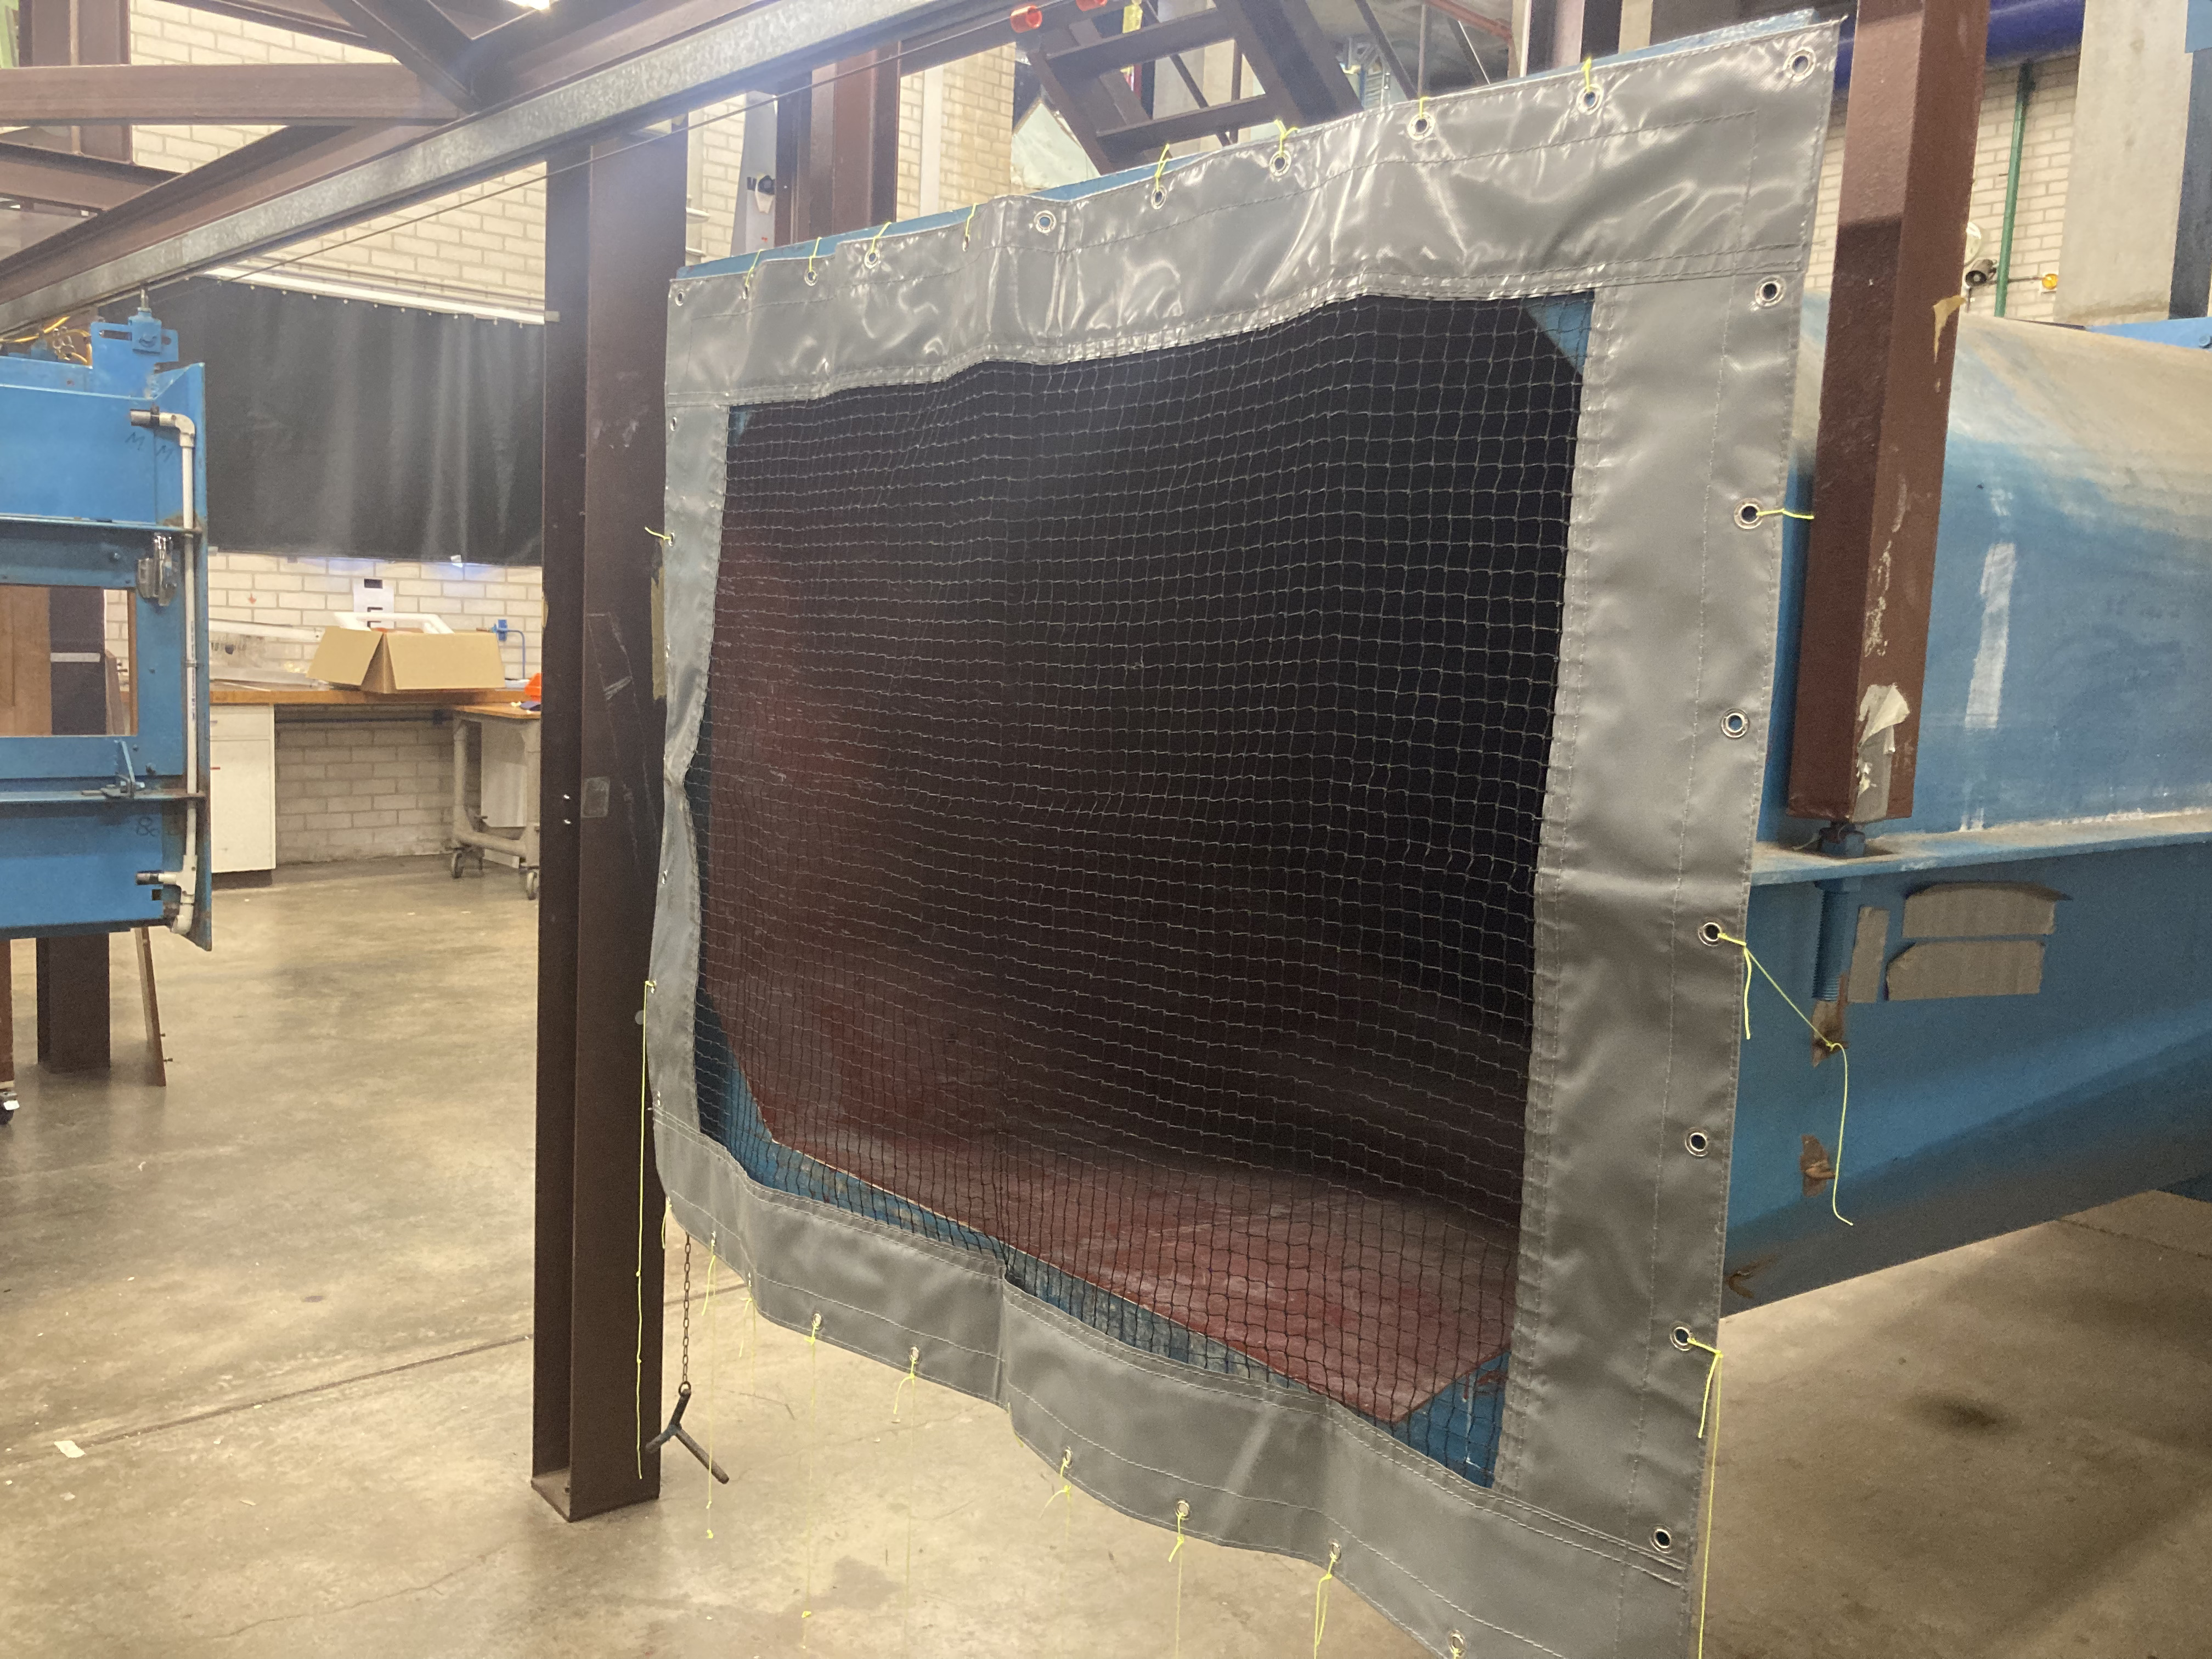
\includegraphics[scale =0.1]{04_Methodology/Figs/windTunnelNet.jpg}
    \caption{Safety net to }
    \label{fig:windTunnelNet}
\end{figure}

\begin{figure}[!ht]
    \centering
    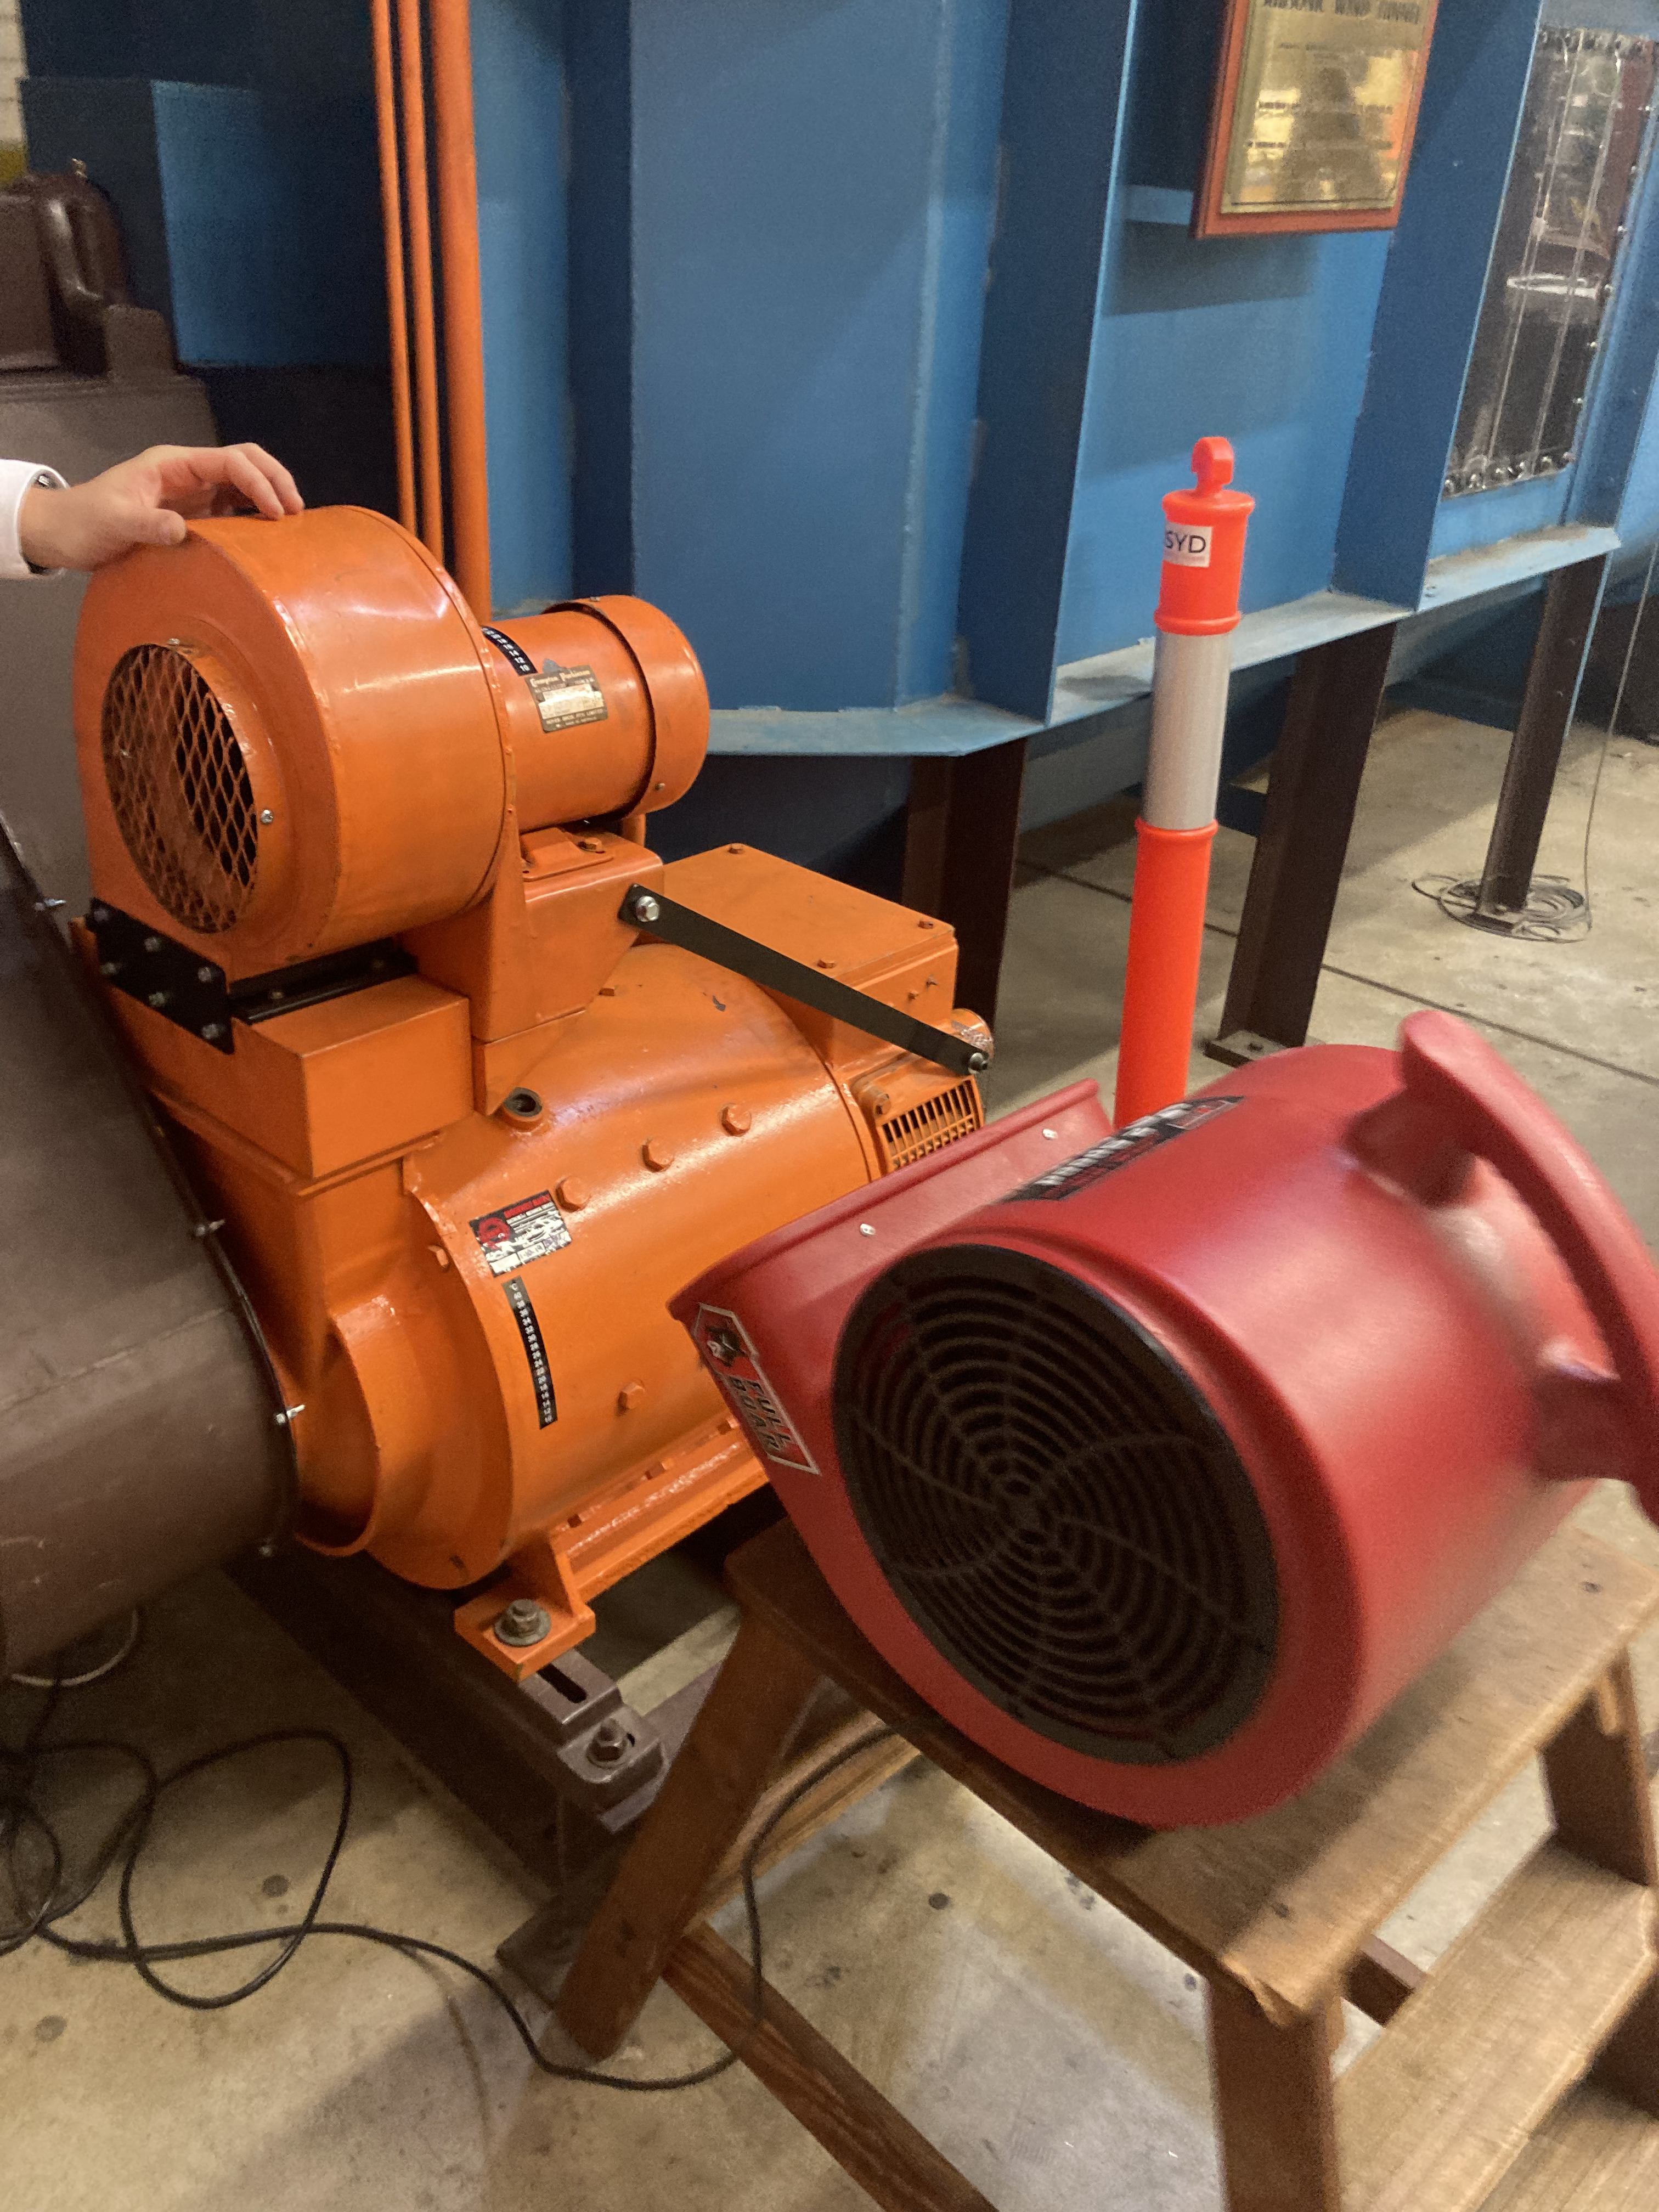
\includegraphics[scale=0.1]{04_Methodology/Figs/cooler.jpg}
    \caption{Caption}
    \label{fig:engineCooler}
\end{figure}

The nano25 load cell was used to record the forces and moments acting on the model about the mounting position at 25$\overline{c}$. 

\begin{figure}[H]
    \centering
    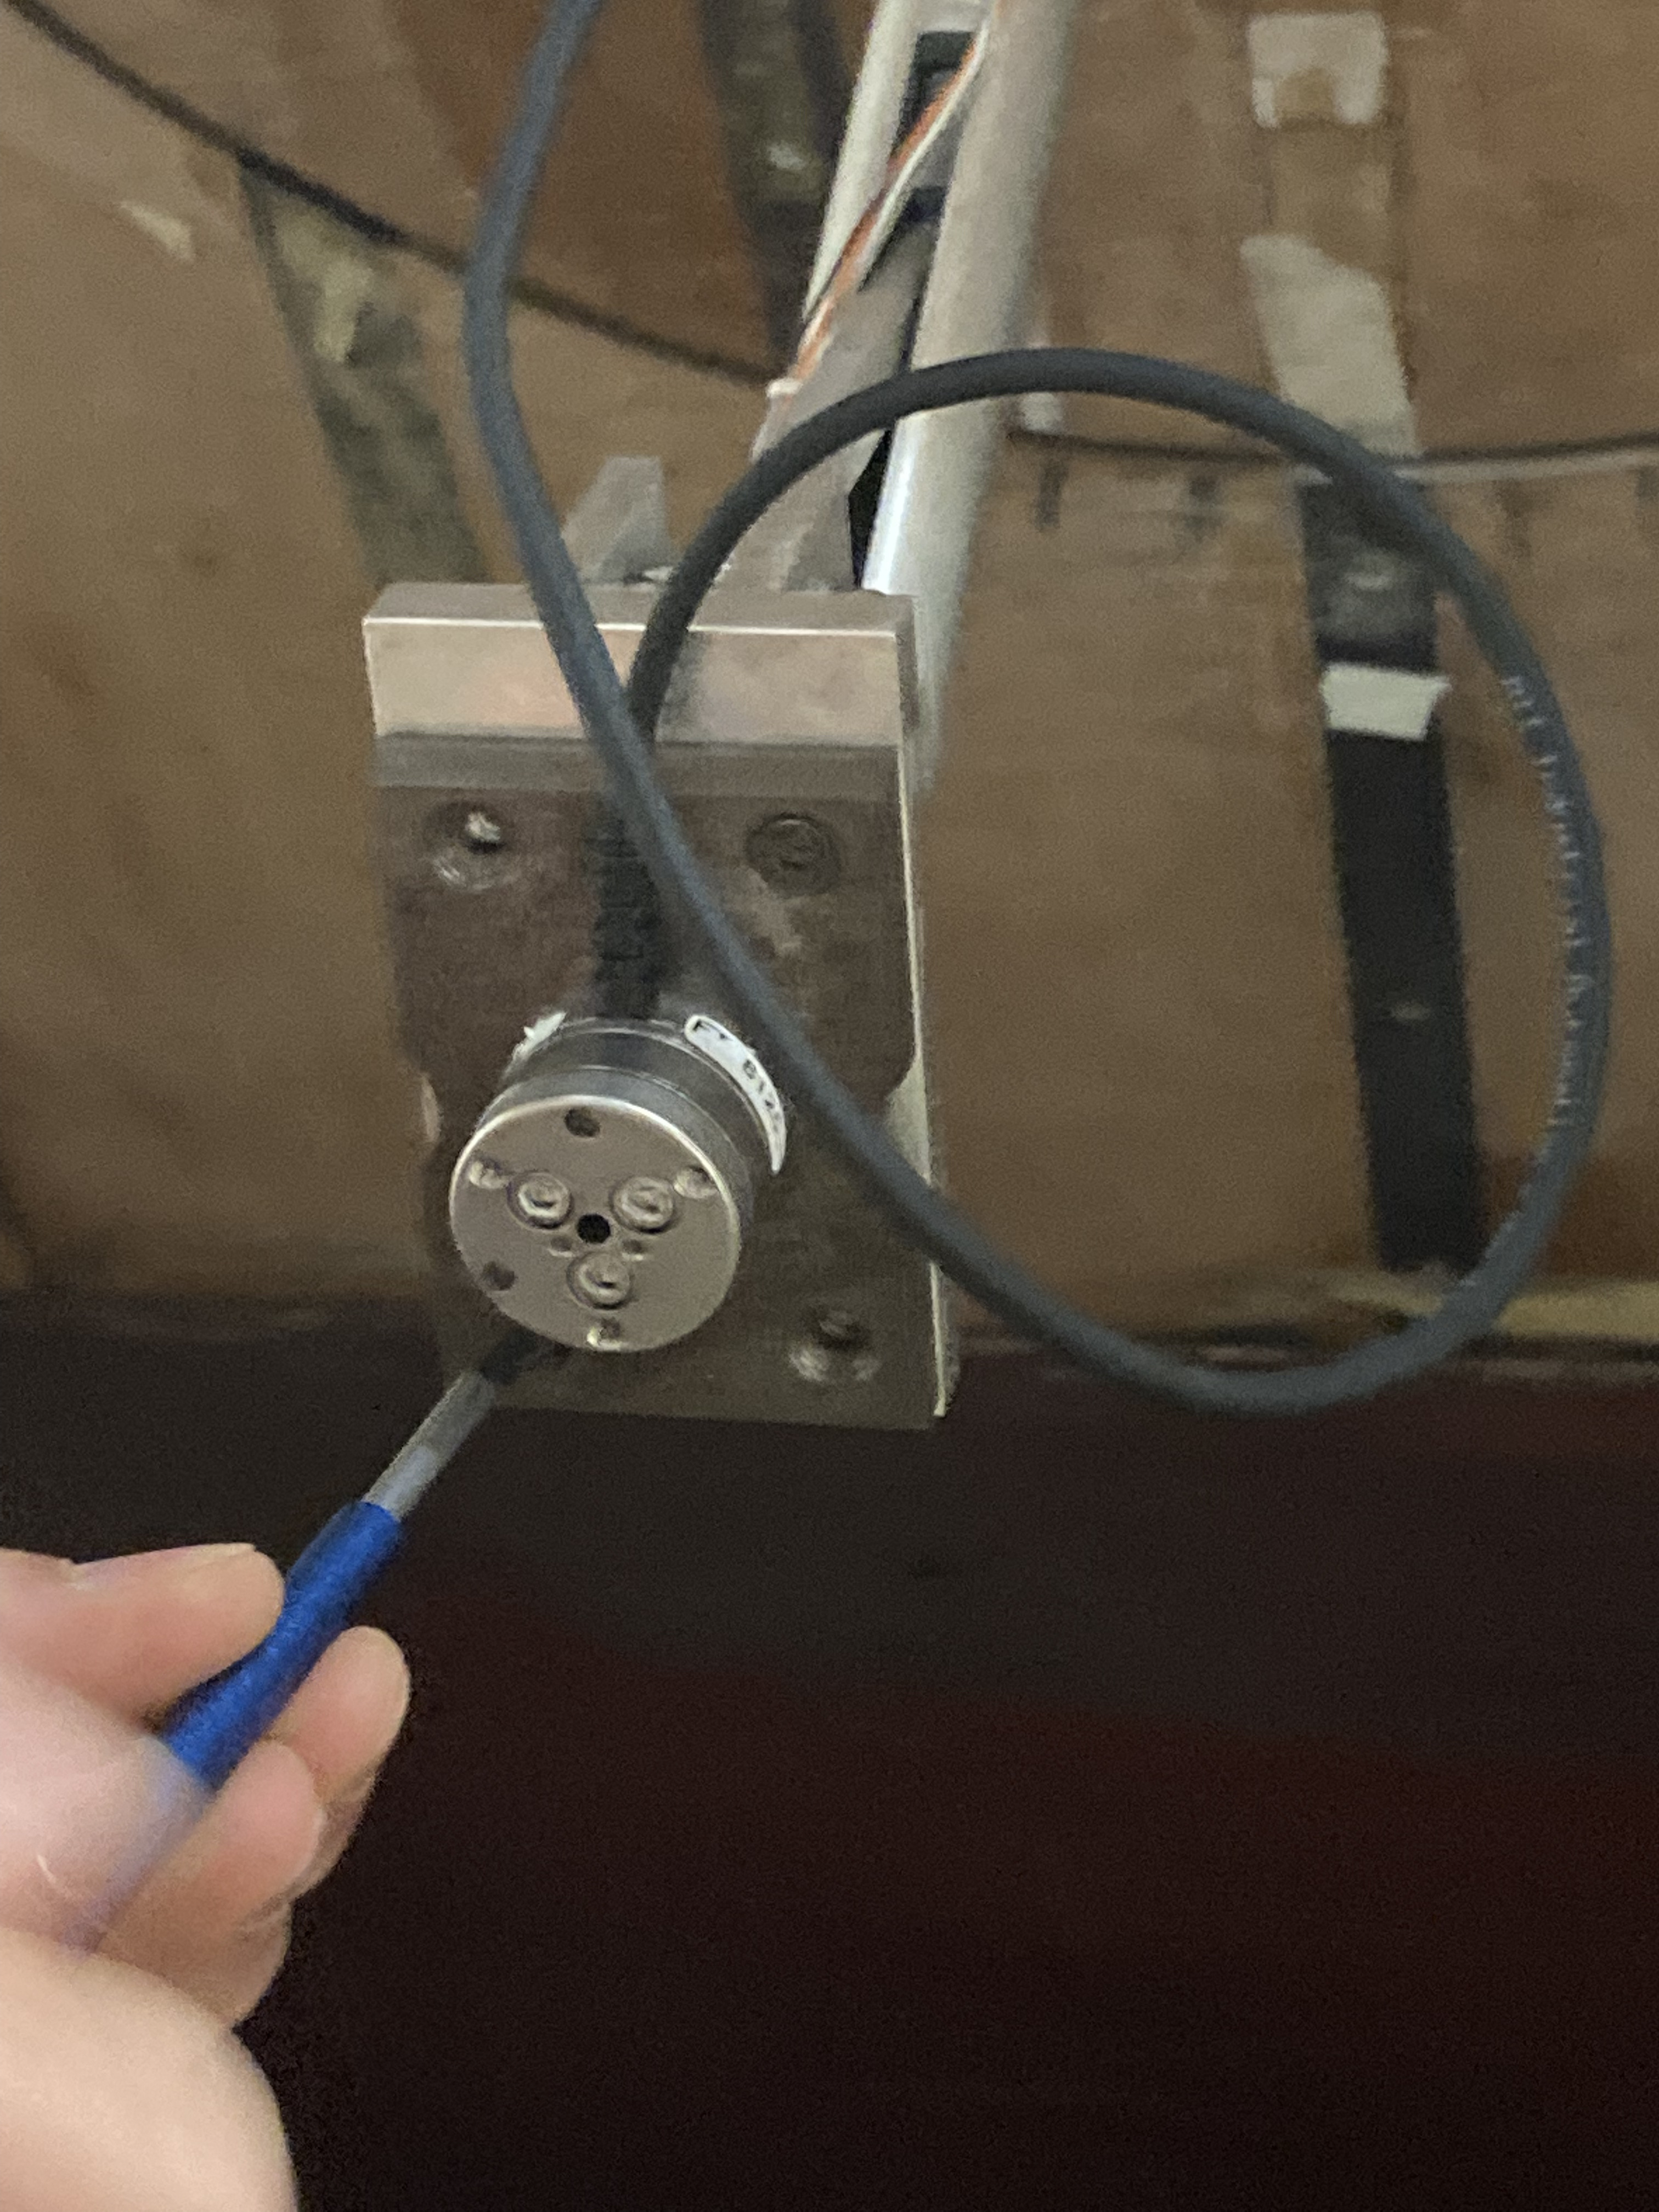
\includegraphics[scale=0.08]{04_Methodology/Figs/loadCellMount}
    \caption{Nano 25 load cell mount}
    \label{fig:LoadCella}
\end{figure}

The model mount was then attached over the load cell. 


\begin{figure}[!ht]
    \centering
    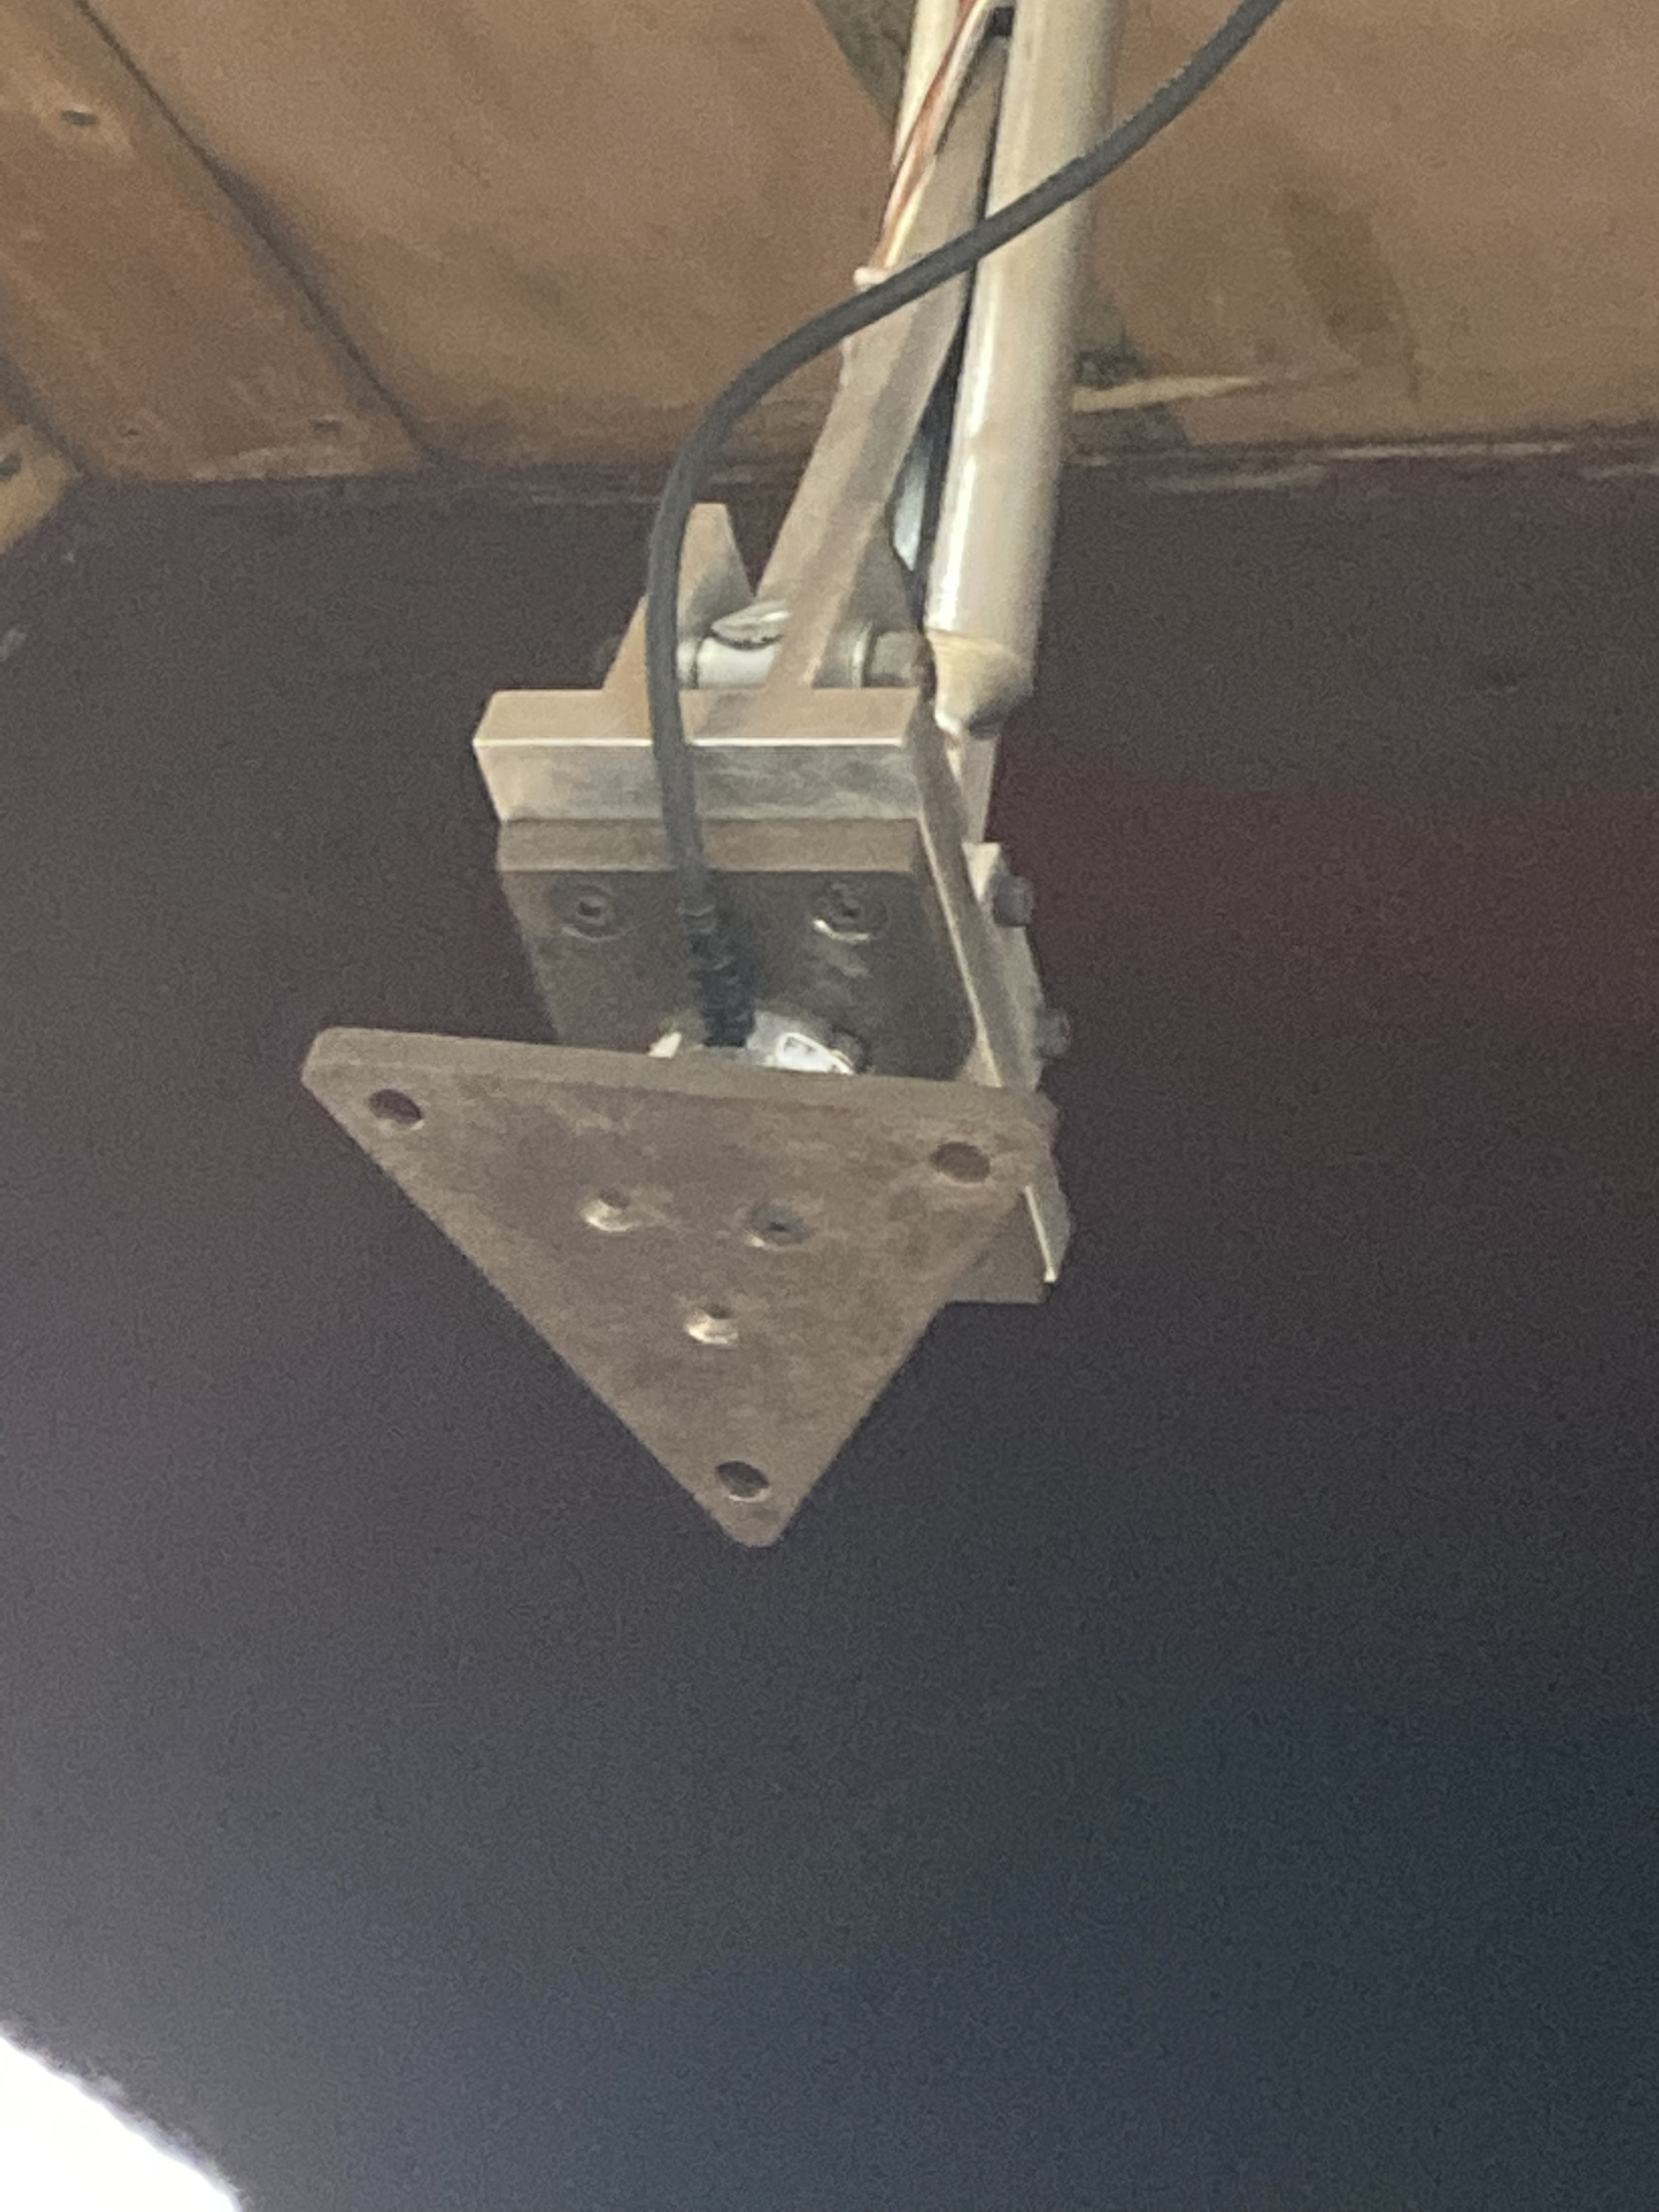
\includegraphics[scale=0.1]{04_Methodology/Figs/mount}
    \label{fig:LoadCellb}
\end{figure}

The model was then attached in three main configurations. These were mounting the propeller without a propeller, in a tractor and pusher configurations.


\begin{figure}[!ht]
     \centering
     \begin{subfigure}[b]{0.3\textwidth}
         \centering
         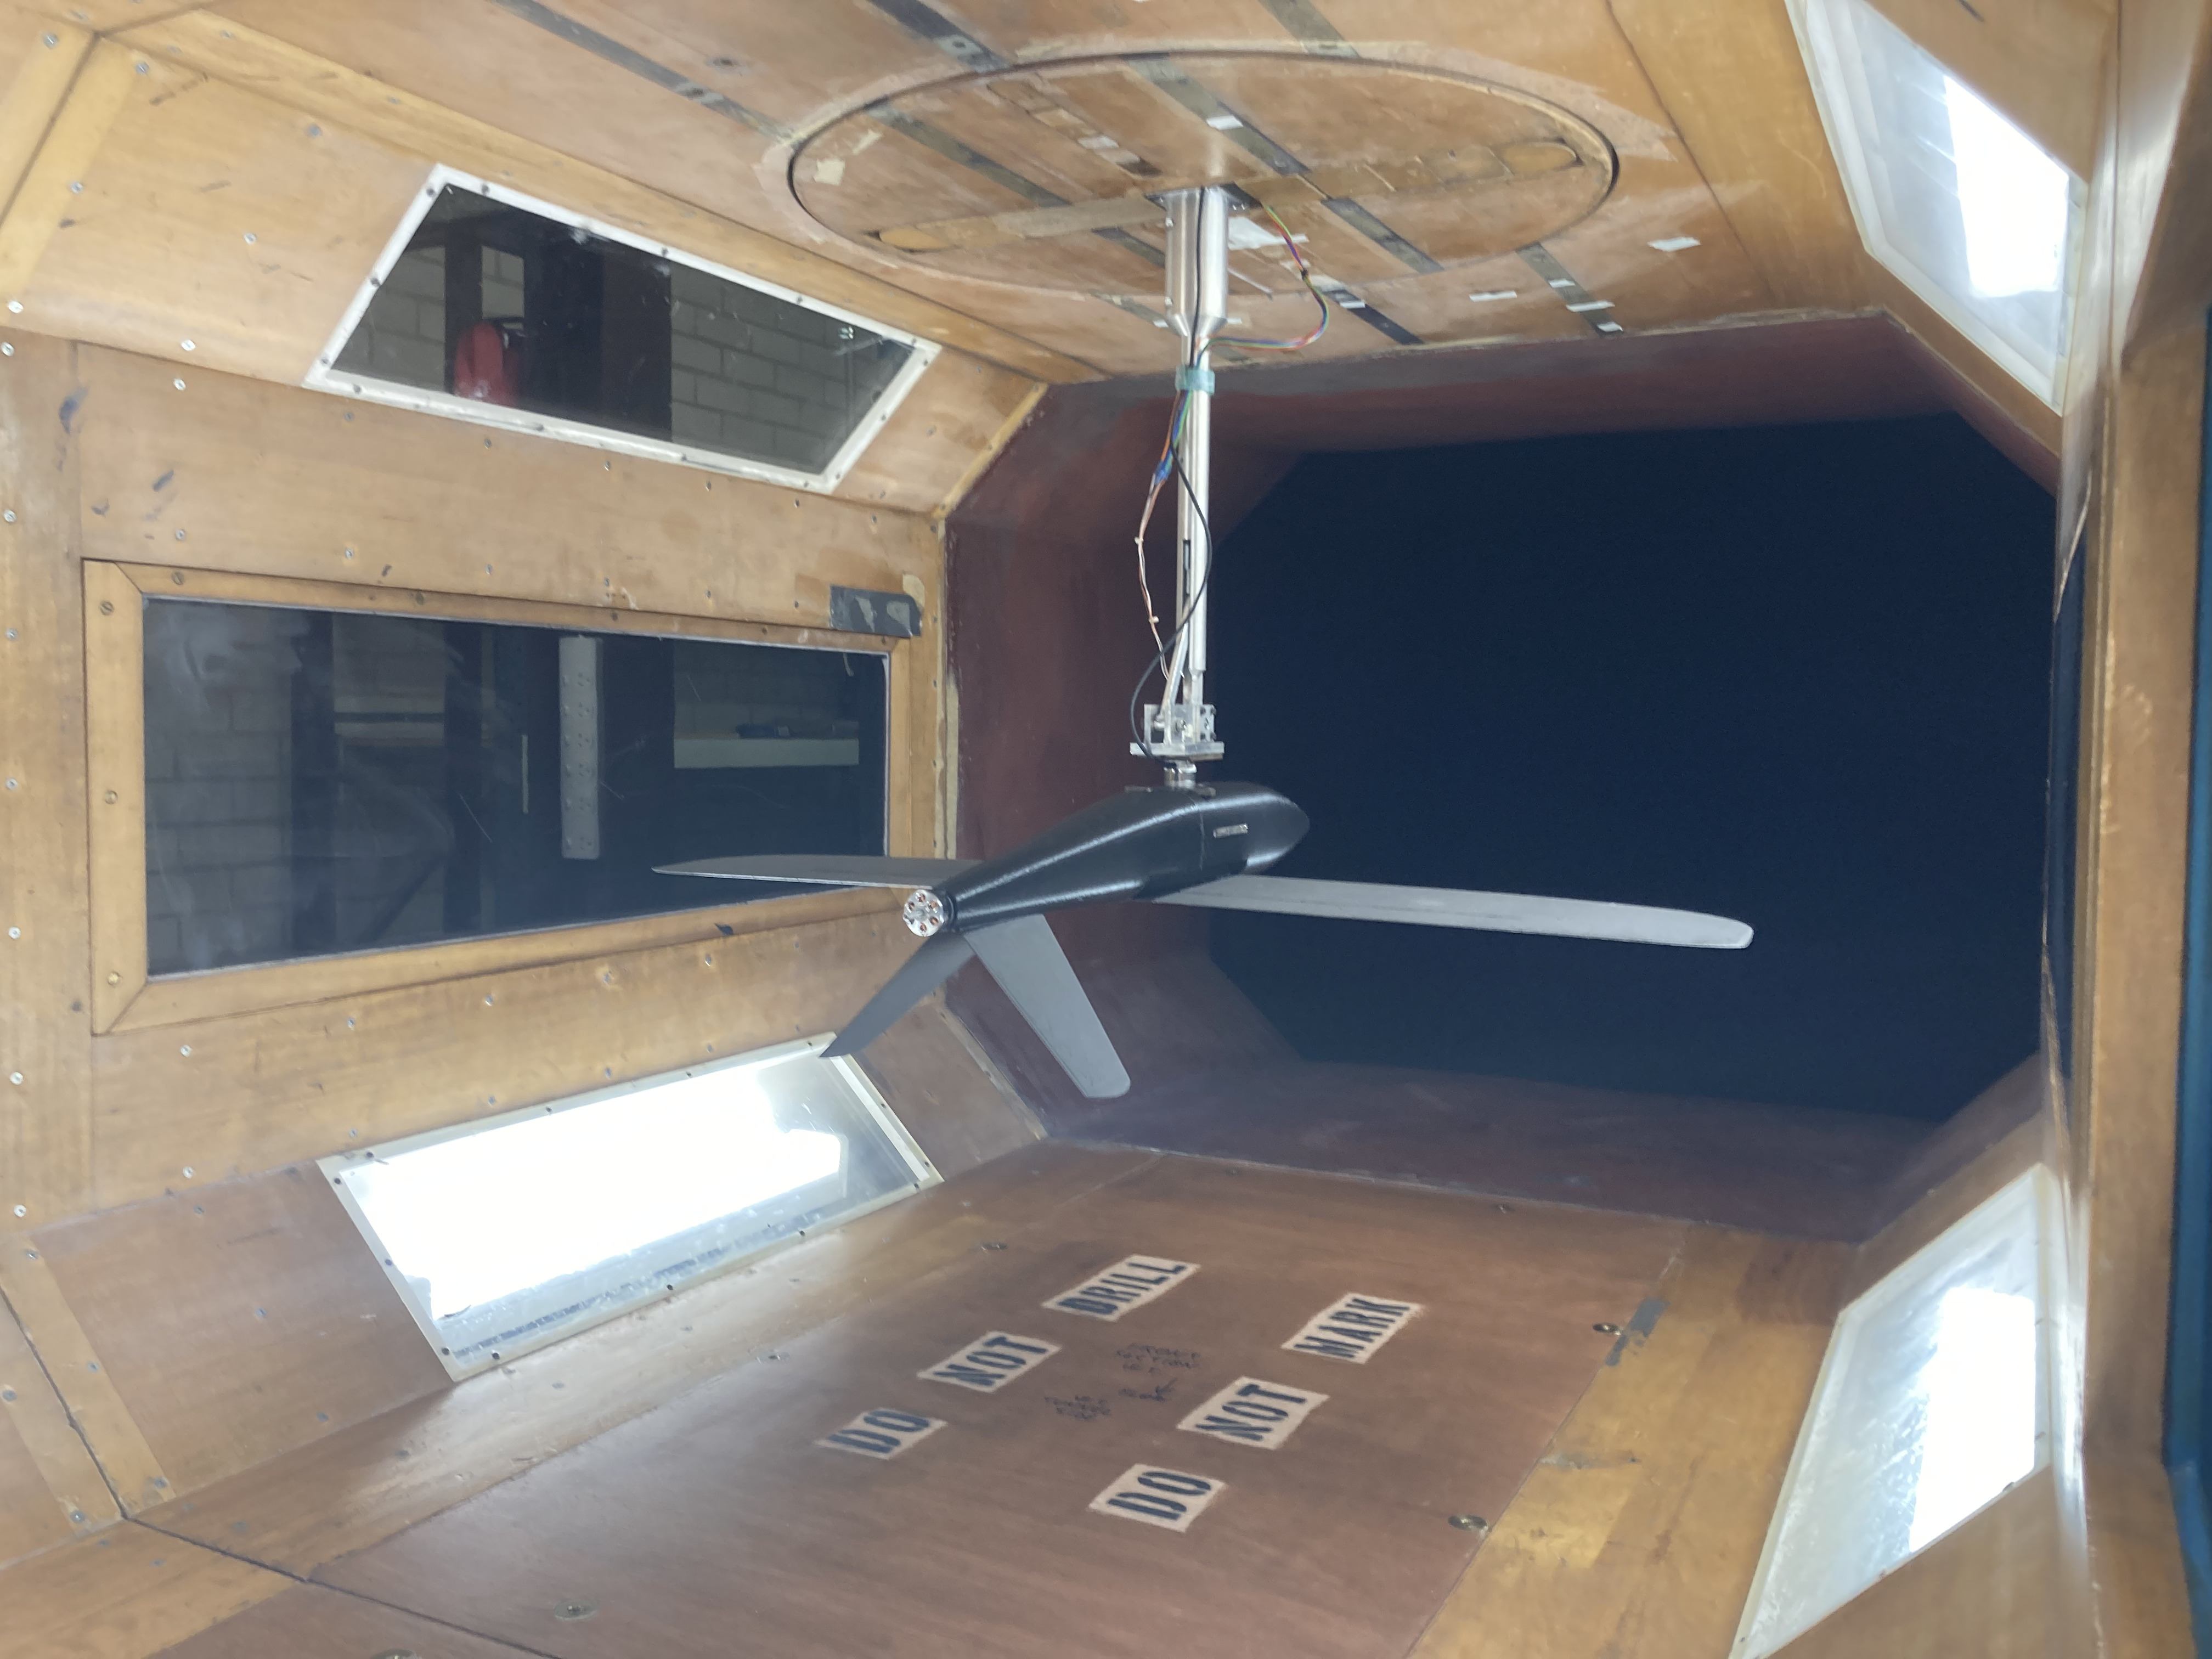
\includegraphics[scale=0.1]{04_Methodology/Figs/noprop}
          \label{fig:noprop}
     \end{subfigure}
     \hfill
     \begin{subfigure}[b]{0.3\textwidth}
             \centering
             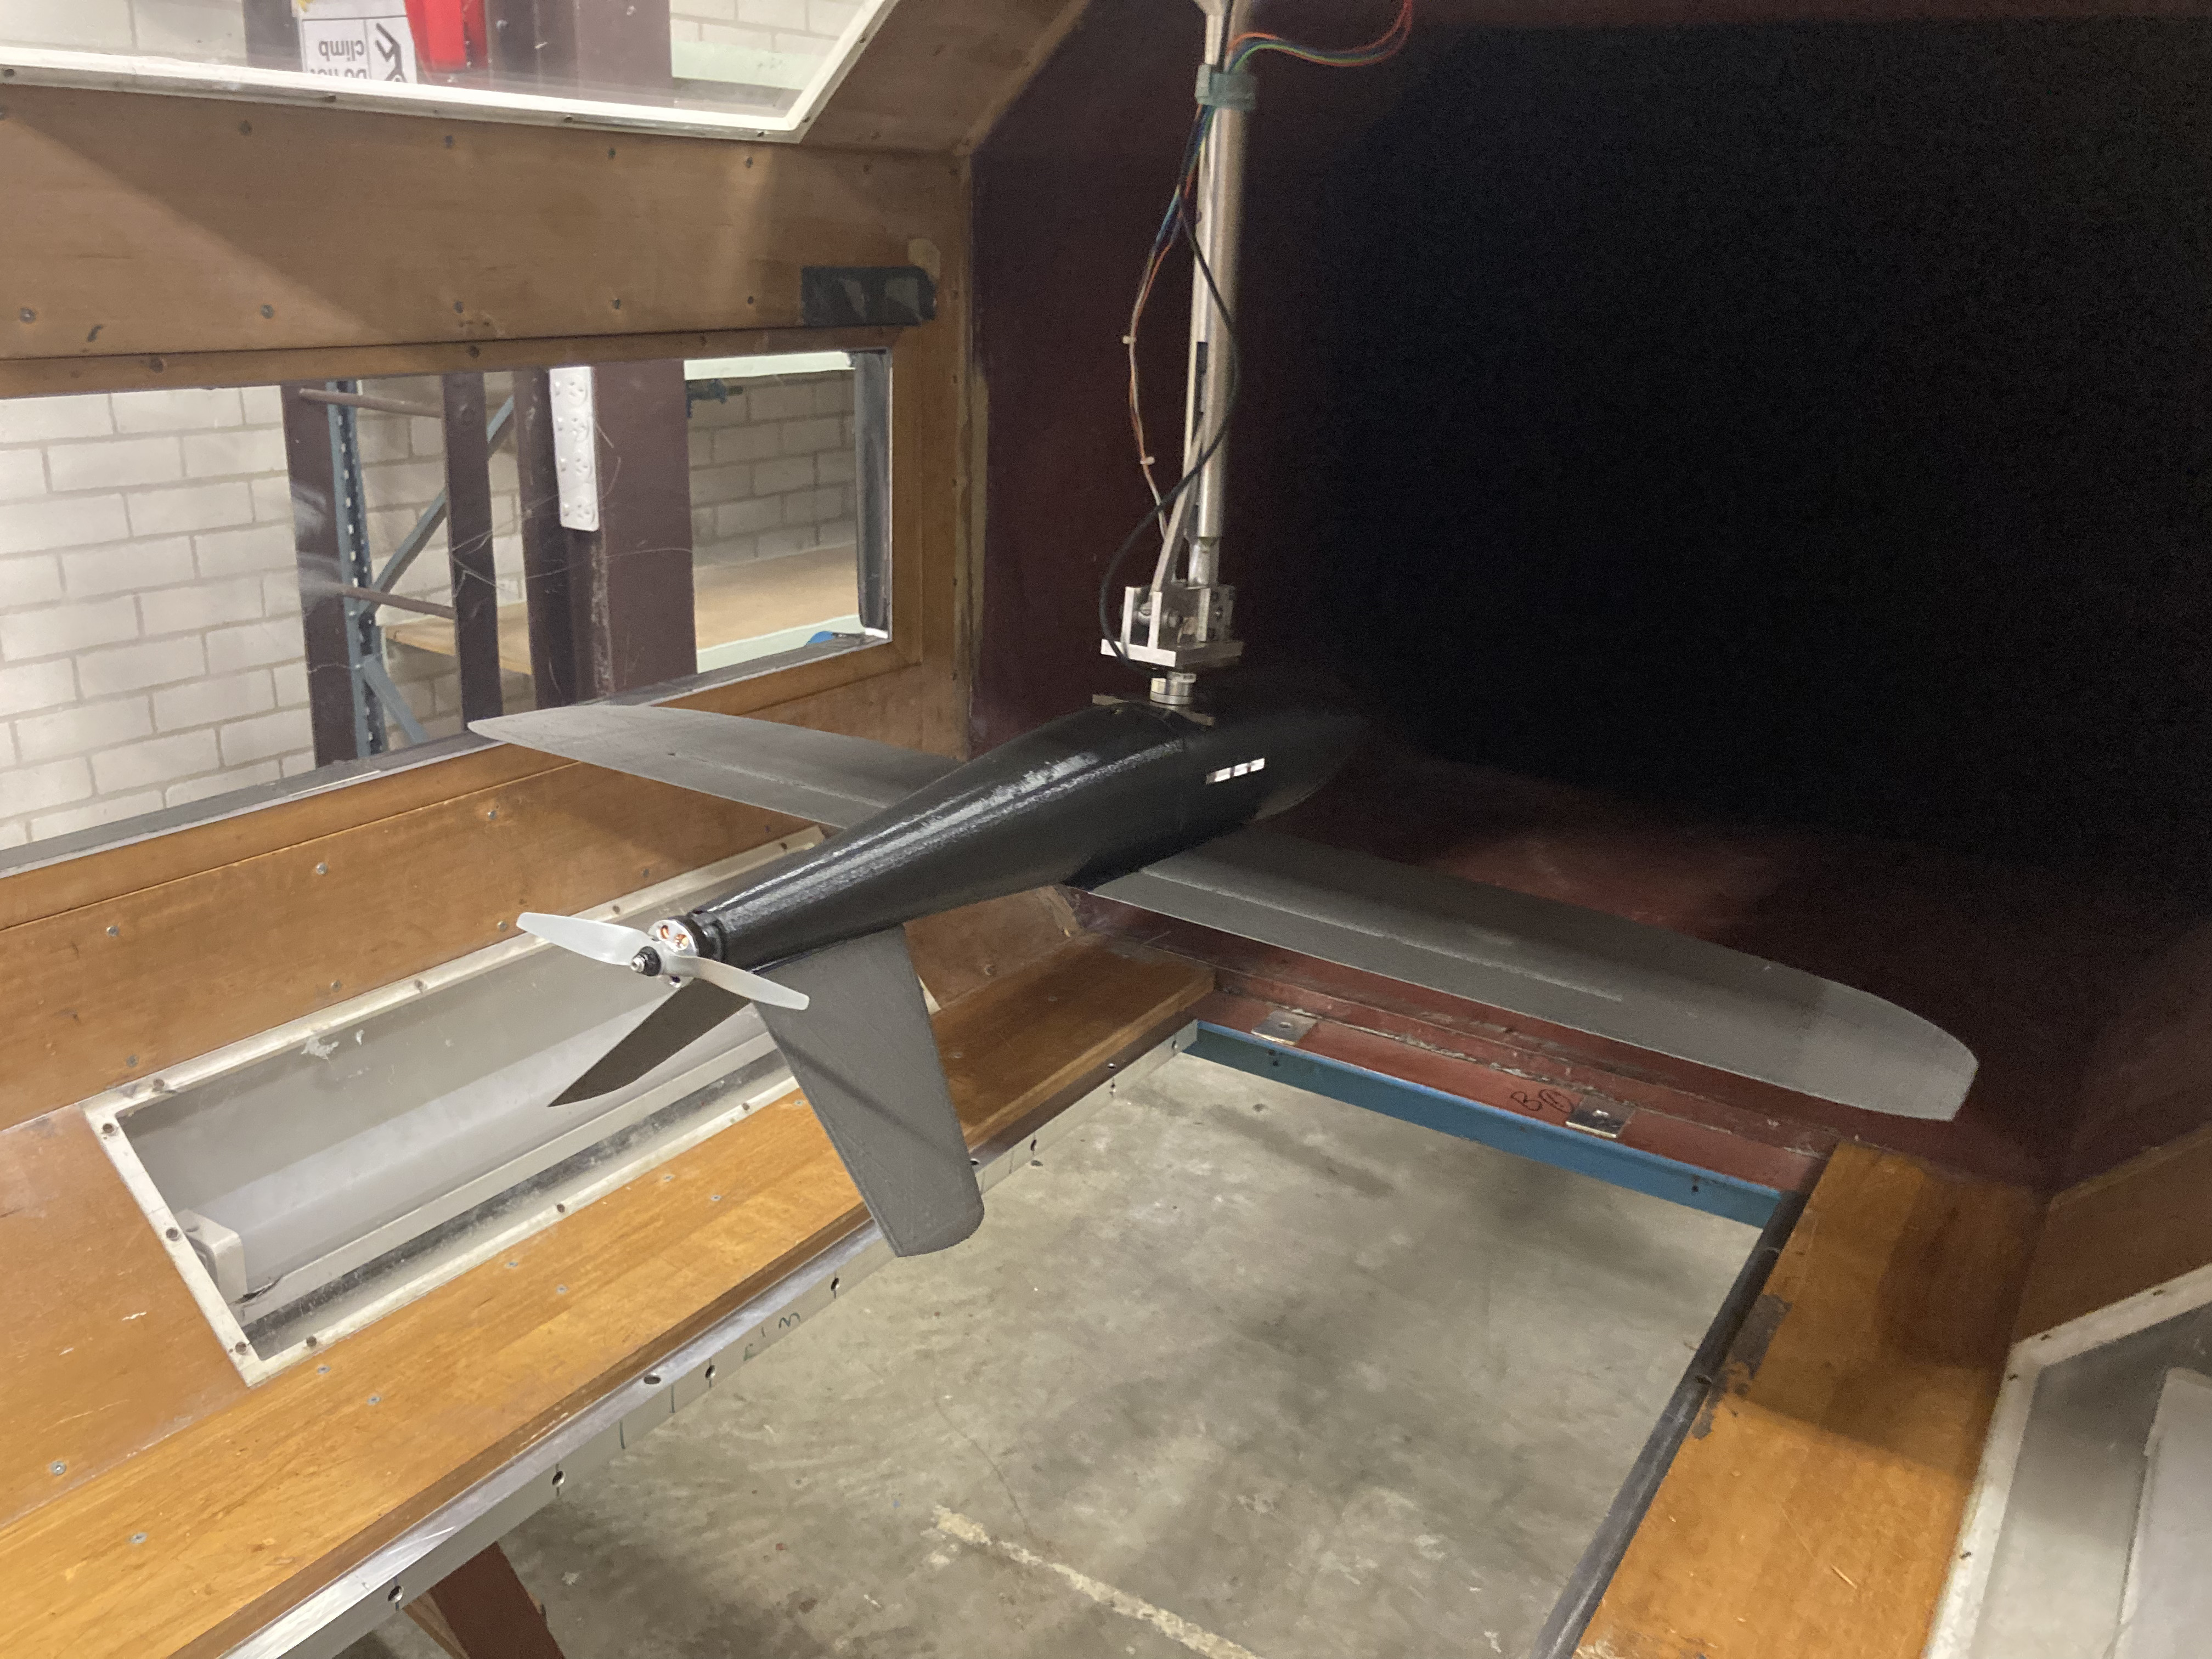
\includegraphics[scale = 0.1]{04_Methodology/Figs/pusher}
             \label{fig:pusher}
     \end{subfigure}
     \hfill
     \begin{subfigure}[b]{0.3\textwidth}
             \centering
             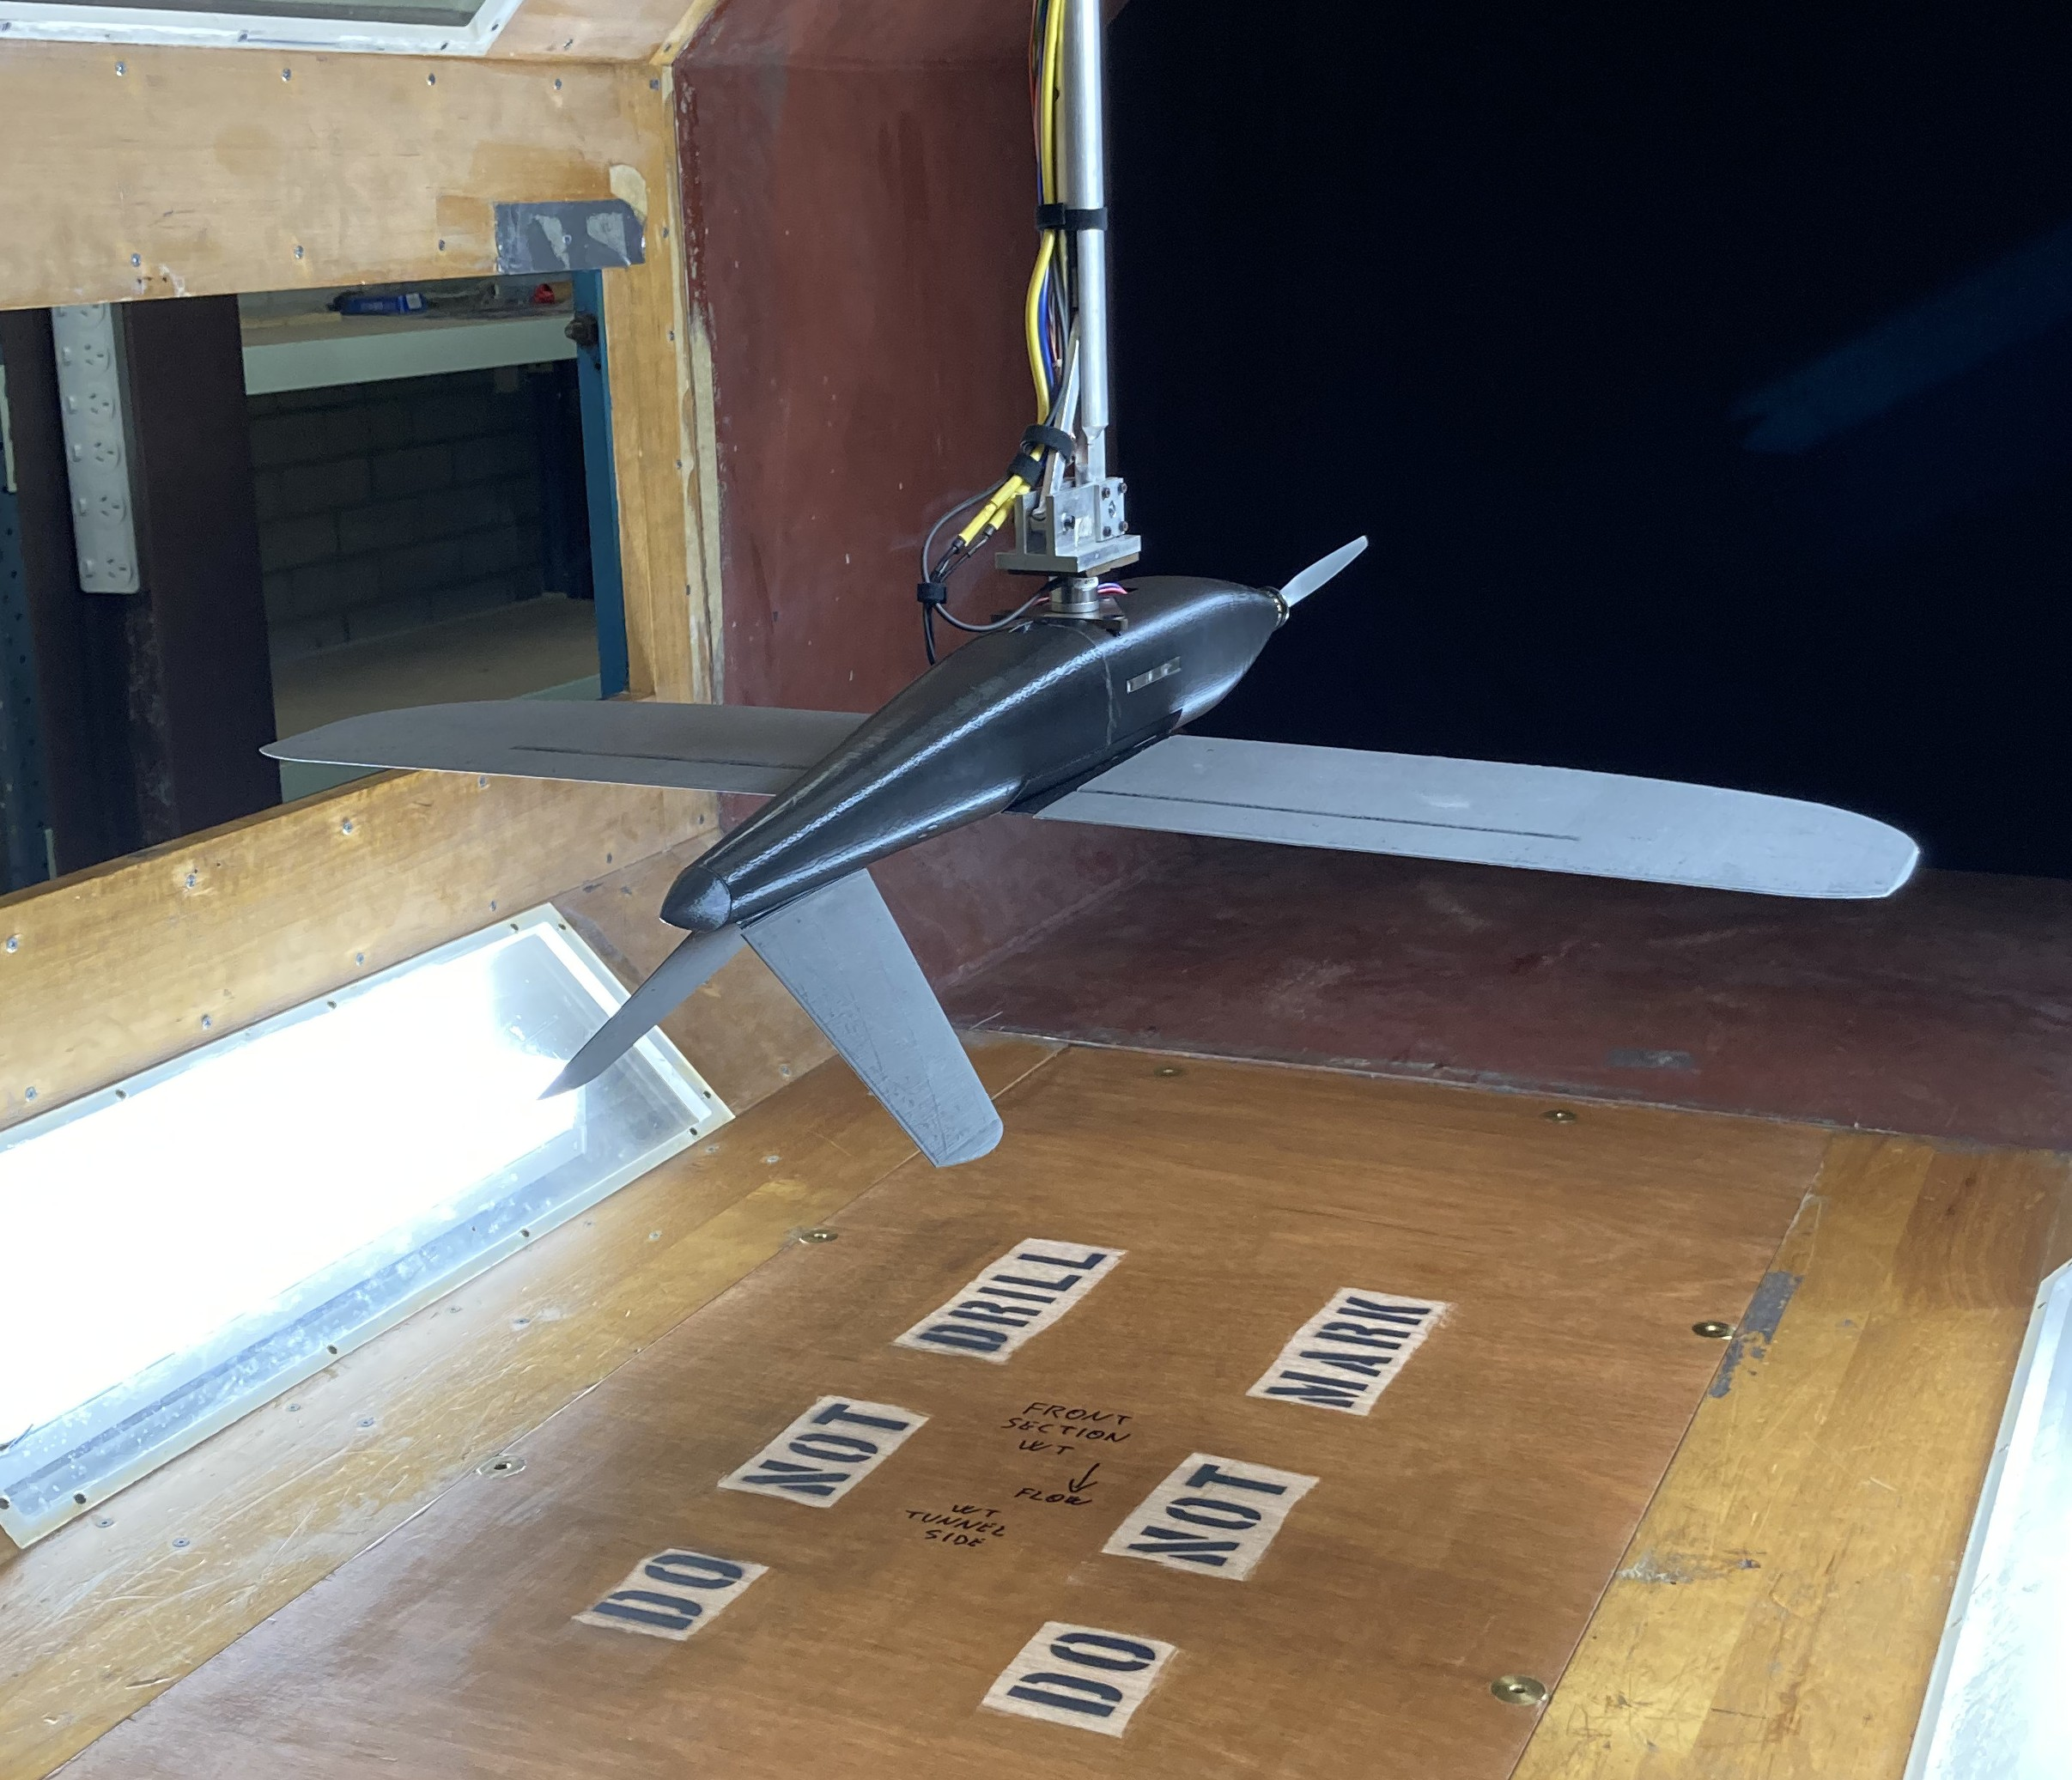
\includegraphics[scale=0.1]{04_Methodology/Figs/tractors}
             \label{fig:tractors}
     \end{subfigure}
        \caption{Examples of MAVs with category}
        \label{fig:typesUsed}
\end{figure}

The wind tunnel was then callibrated for wind speed, atmospheric conditions and angles of attack. The mount used for the model was double checked using a pitch gauge to ensure the angle of attack was correct. 
\begin{figure}
    \centering
    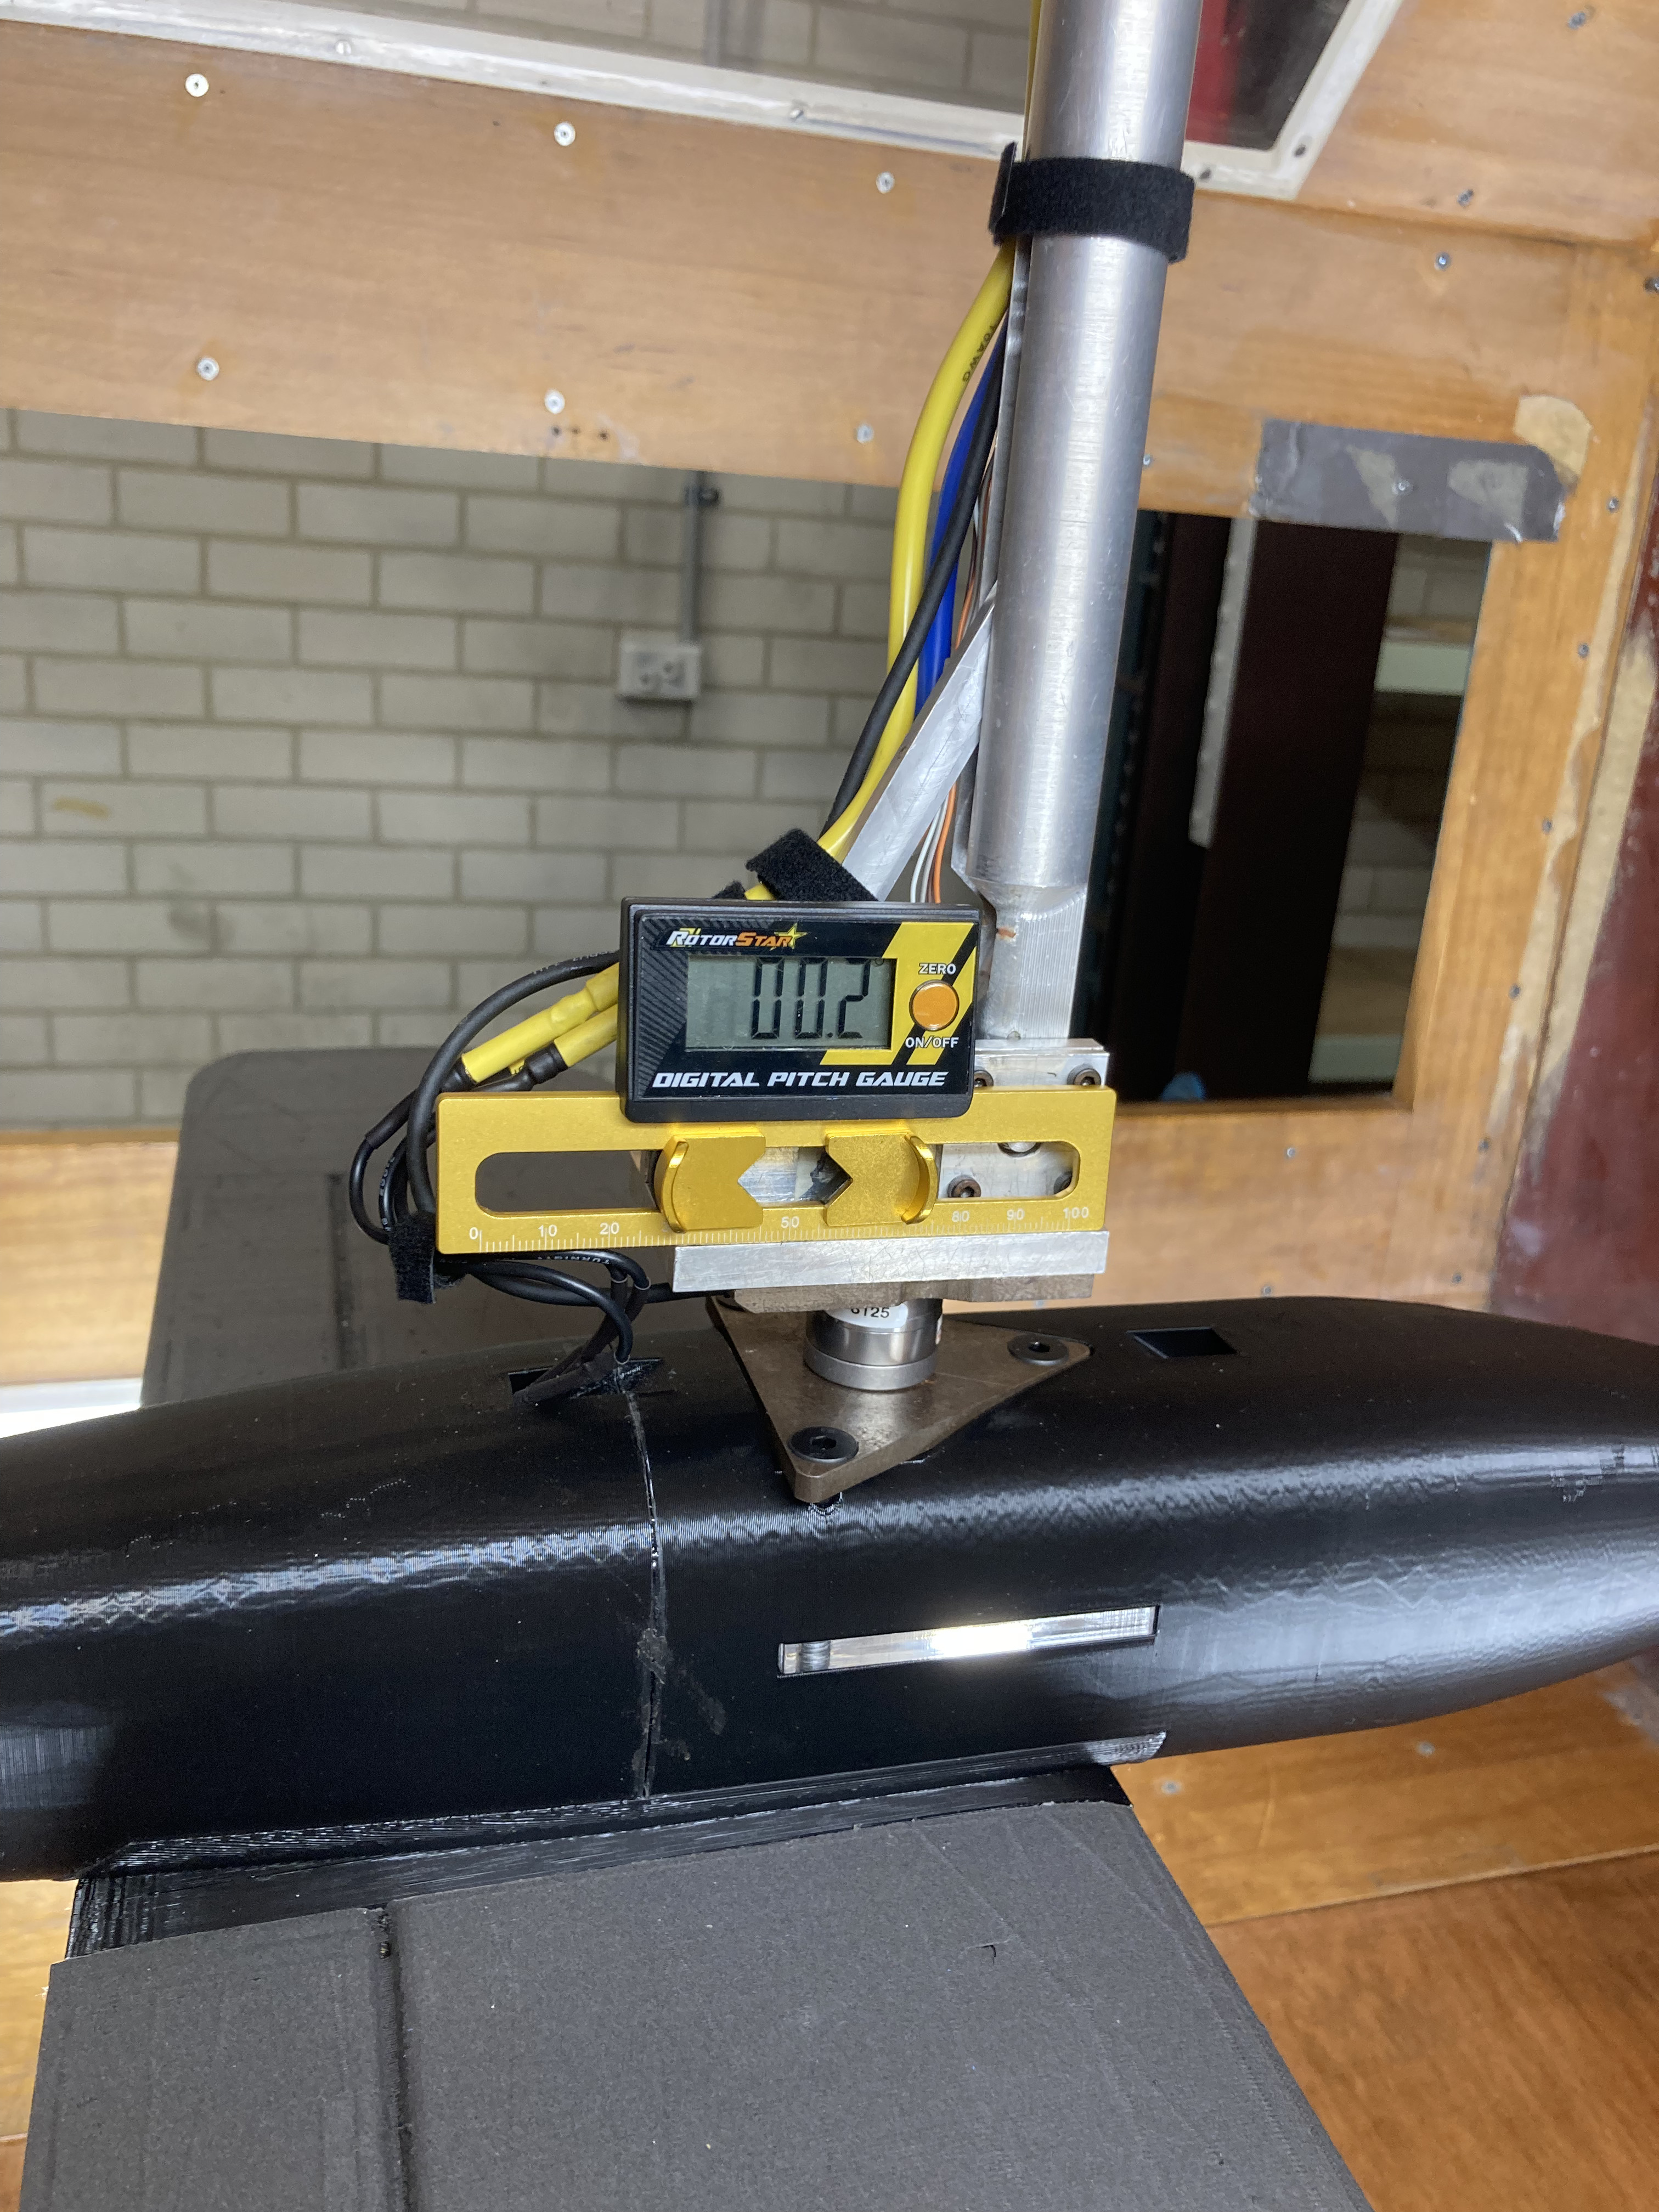
\includegraphics[scale=0.1]{04_Methodology/Figs/pitchGauge.jpg}
    \caption{Callibrating pitch of model mount to ensure Aoa is accurate}
    \label{fig:pitchGauge}
\end{figure}

When using the prop the motor was supplied with a 7.4V battery and the RPM was set to $\approx 6000 RPM$, $\approx 9000RPM$ and $\approx 11000 RPM$. 






\section{Stability Calculation}
In order to determine the stability of the model in all the tested configurations the stability deratives of the model had to be determined. Data from the nano 25 load cell was used to determine the loads and moments acting on the model about the mounting point. These values were transformed \todo{right word?} to the neutral point of the model at 20$\overline{c}$. The aerodynamic coefficients were determined using equations \ref{eqn:lift} to \ref{eqn:drag} and the moment coefficients about the pitch, yaw and roll axis were calculated using Equations \ref{eqn:pitching} to \ref{eqn:yaw}. 






\graphicspath{{./Figs/}}

\chapter{Results and Discussion} 

\section{Wind Tunnel Results}
This chapter outlines the final wind tunnel results for all three main configurations; tractor, pusher and no propeller. It outlines the main trends in the stability coefficients Cl, Cn, and Cm corresponding to the MAV model's roll, yaw and pitch. These results are analysed with critical observations and trends identified. A validation of the wind tunnel results is also conducted with VAP 3.5 to compare the accuracy of the results obtained with any discrepancies explained.

\todo{Table of variables/geometry which defines the MAV}


\subsection{Aerodynamic Coefficient of Lift}
\Cref{fig:Cl_10ms_6000} and \Cref{fig:Cl_10ms_11000} show that as the motor speed increases from 6000RPM to 11000RPM the coefficient of lift increases slightly for both the tractor and pusher configurations. As typically seen in aircraft\todo{add citation}, the lift curve also does not drop off. The tractor configuration sees an increase in the lift coefficient beyond the stall point, while the pusher configuration has a linear decrease in the lift coefficient beyond the stall point. Increasing the airspeed to 20m$s^{-1}$ at the higher 11000RPM speed delays the MAV model's stall as the angle of attack increases in all configurations. Increasing the airspeed when the motor is at 6000RPM increases the max coefficient of lift seen for the pusher configuration \todo{ADD VALUES} and delays stall. The tractor configuration has a deeper stall beyond the stall point when airspeed is at 20m$s^{-1}$, and leads to a more unrecoverable aircraft if stall were to occur as the MAV would experience extremely high angles of attack. It also gives little room for error or warning in order to correct the MAVs position in order to avoid a stall. These trends due to airspeed are shown between \Cref{fig:Cl_10ms_6000} and \Cref{fig:Cl_20ms_6000} as well as between \Cref{fig:Cl_10ms_11000} and \Cref{fig:Cl_20ms_11000}.

\begin{figure}[H]
    \centering
    \begin{subfigure}[b]{0.467\textwidth}
        \centering
        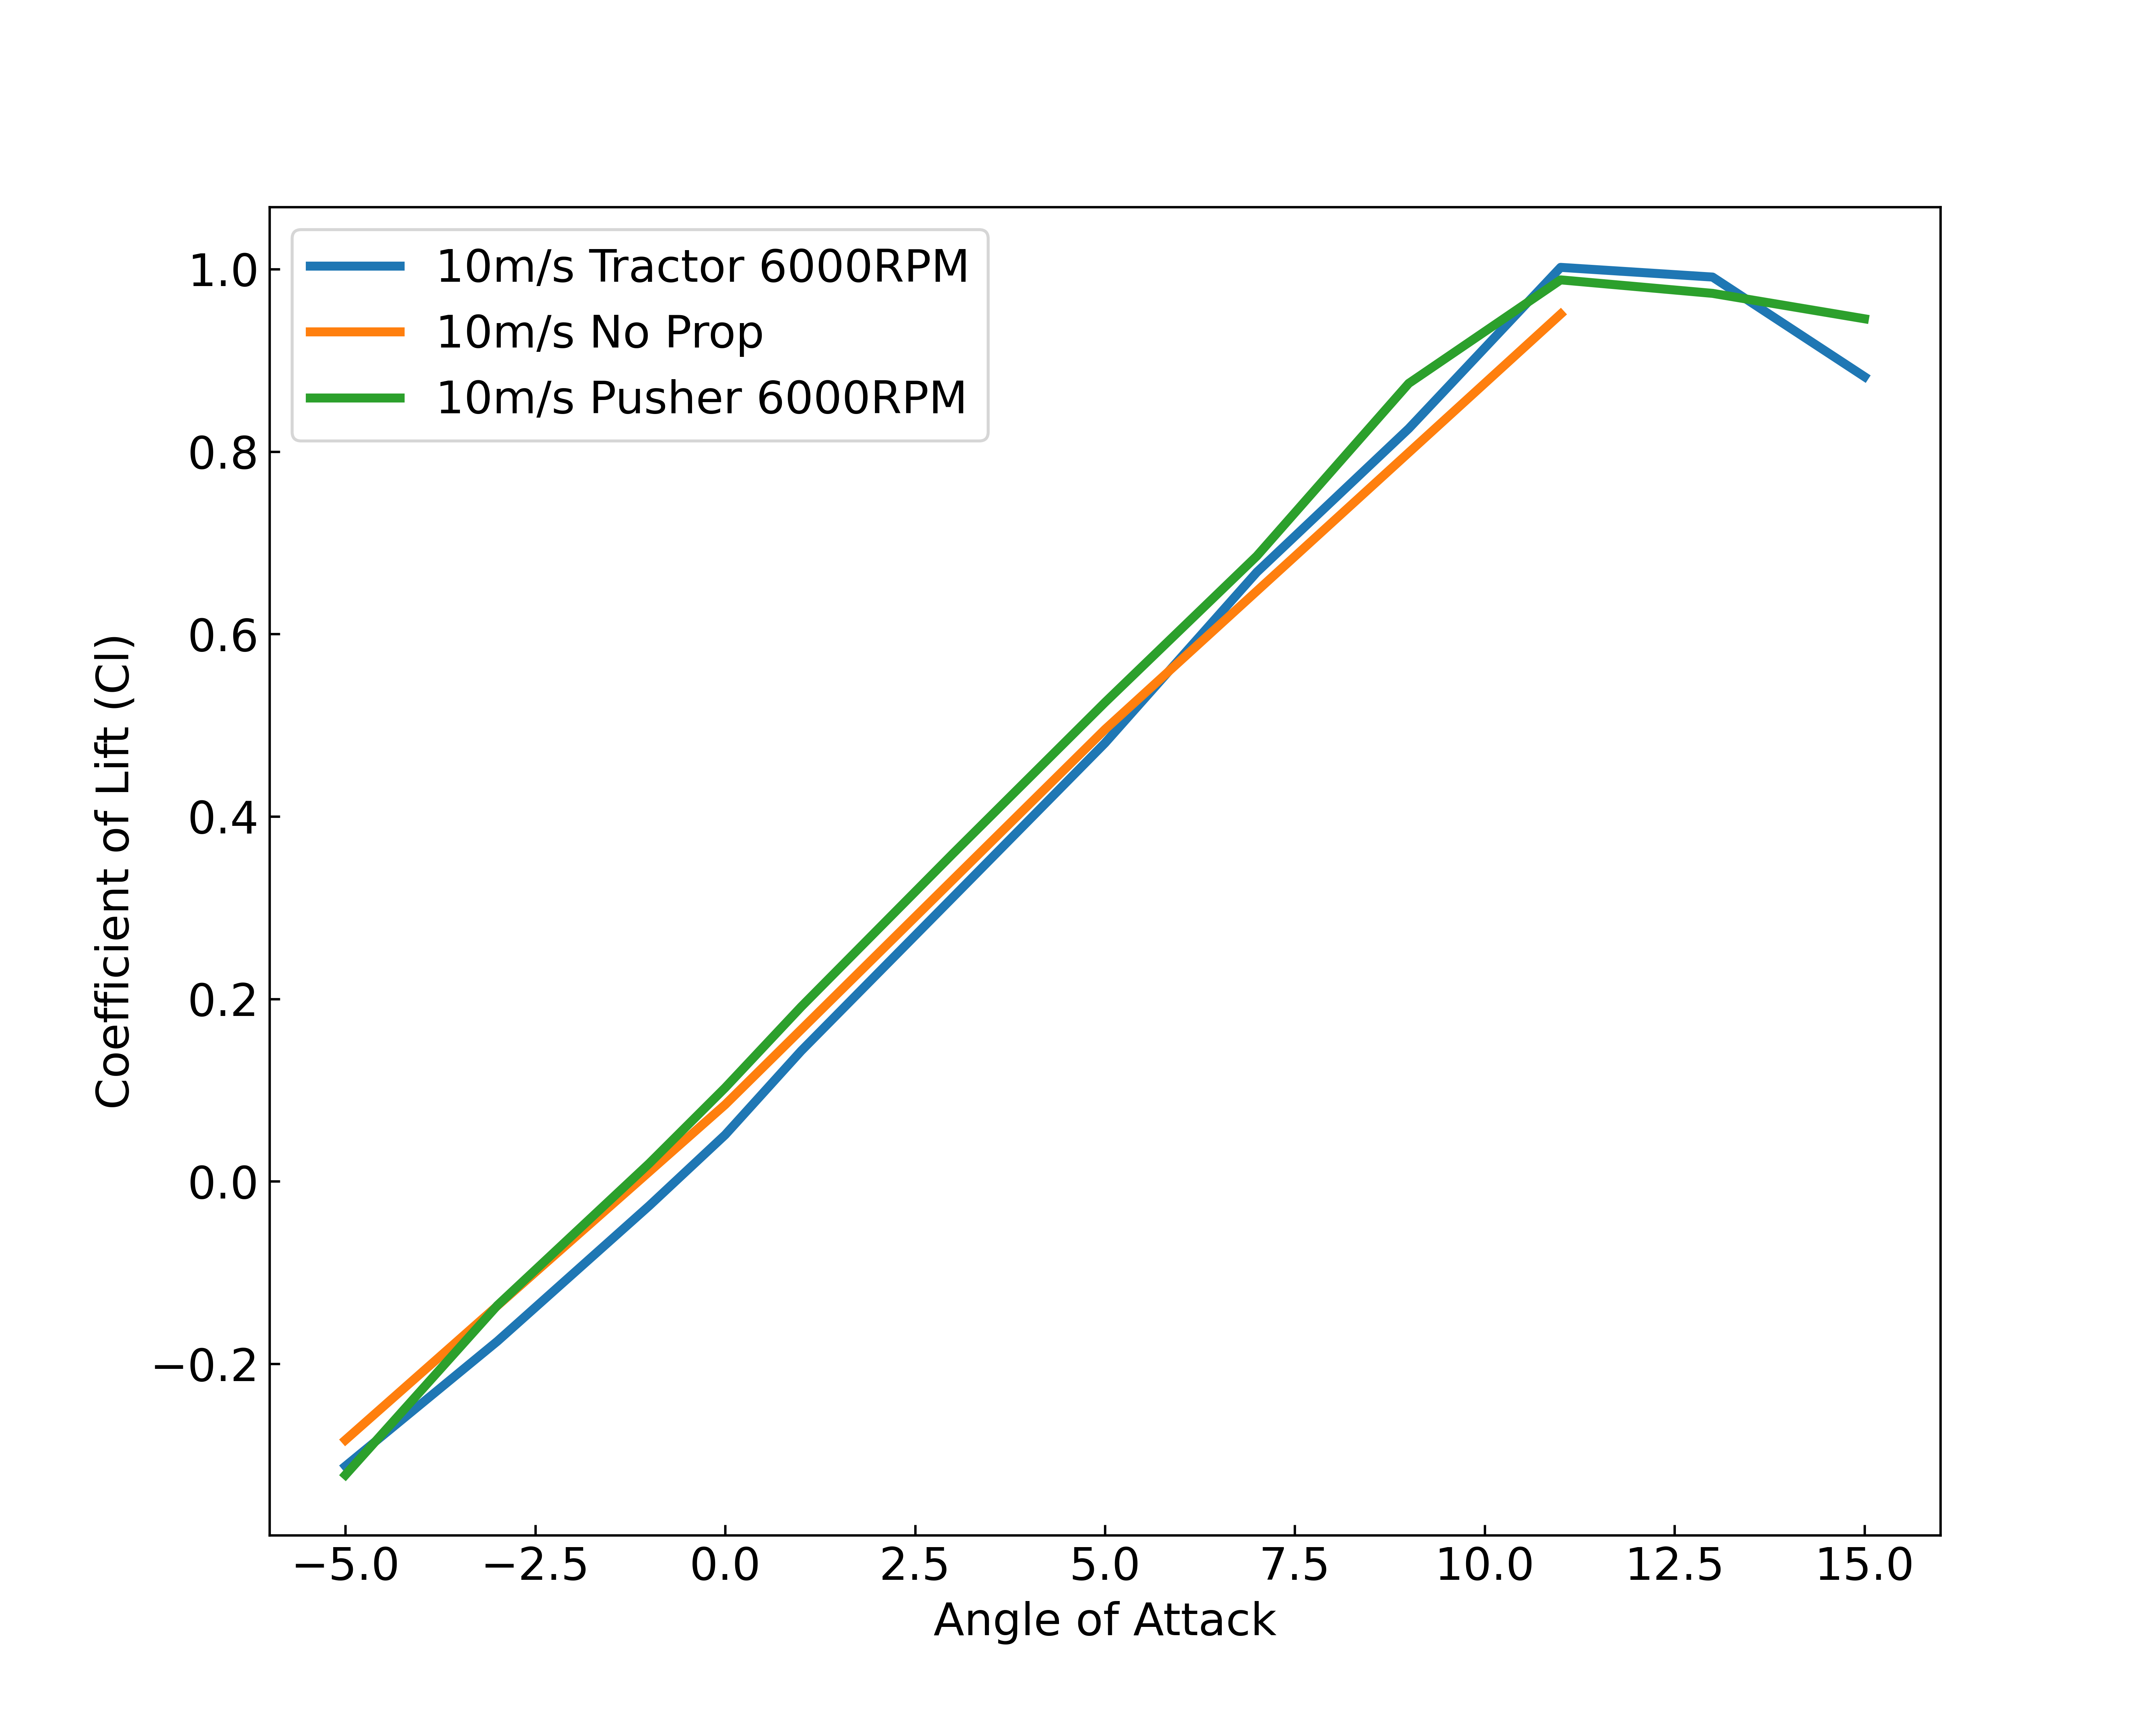
\includegraphics[width=\textwidth]{05_Results/Figs/Cl/10ms_6000RPM_Cl.png}
        \caption{Coefficient of lift at 10m/s airspeed and 6000RPM motor speed}
        \label{fig:Cl_10ms_6000}
    \end{subfigure}
    \begin{subfigure}[b]{0.467\textwidth}
        \centering
        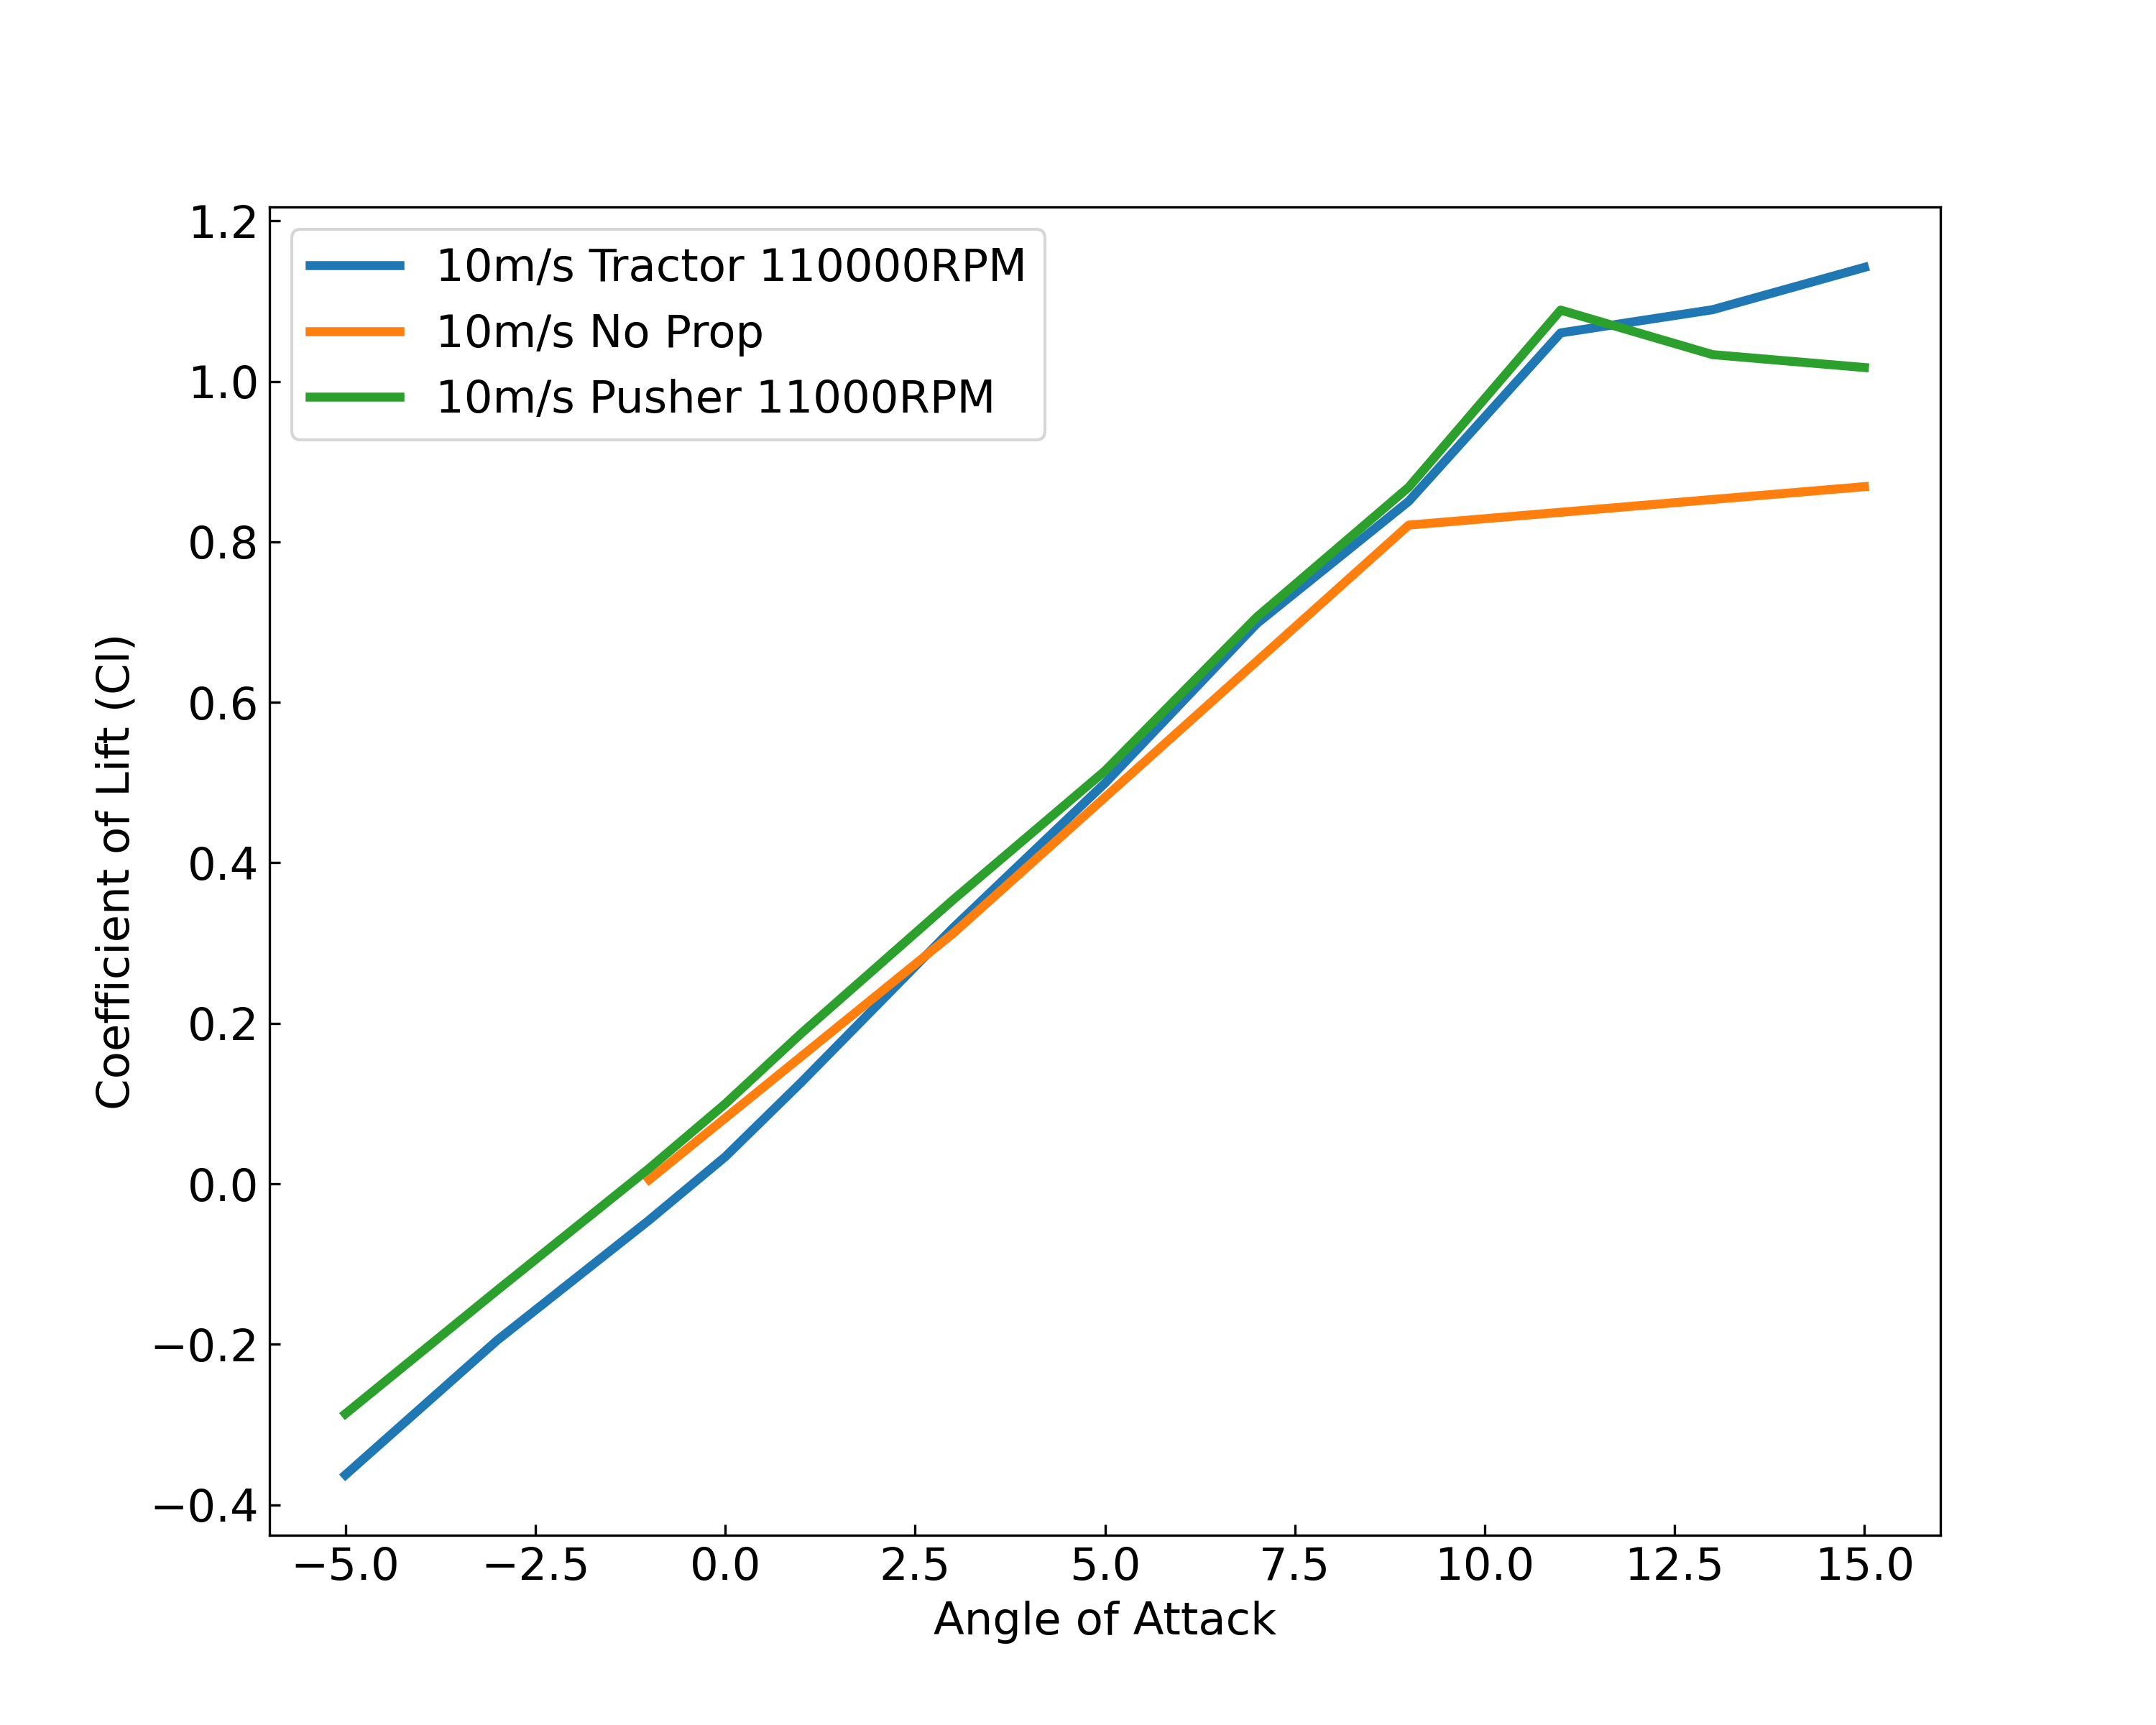
\includegraphics[width=\textwidth]{05_Results/Figs/Cl/10ms_110000RPM_Cl.png}
        \caption{Coefficient of lift at 10m/s airspeed and 11000RPM motor speed}
        \label{fig:Cl_10ms_11000}
    \end{subfigure}
    \begin{subfigure}[b]{0.467\textwidth}
        \centering
        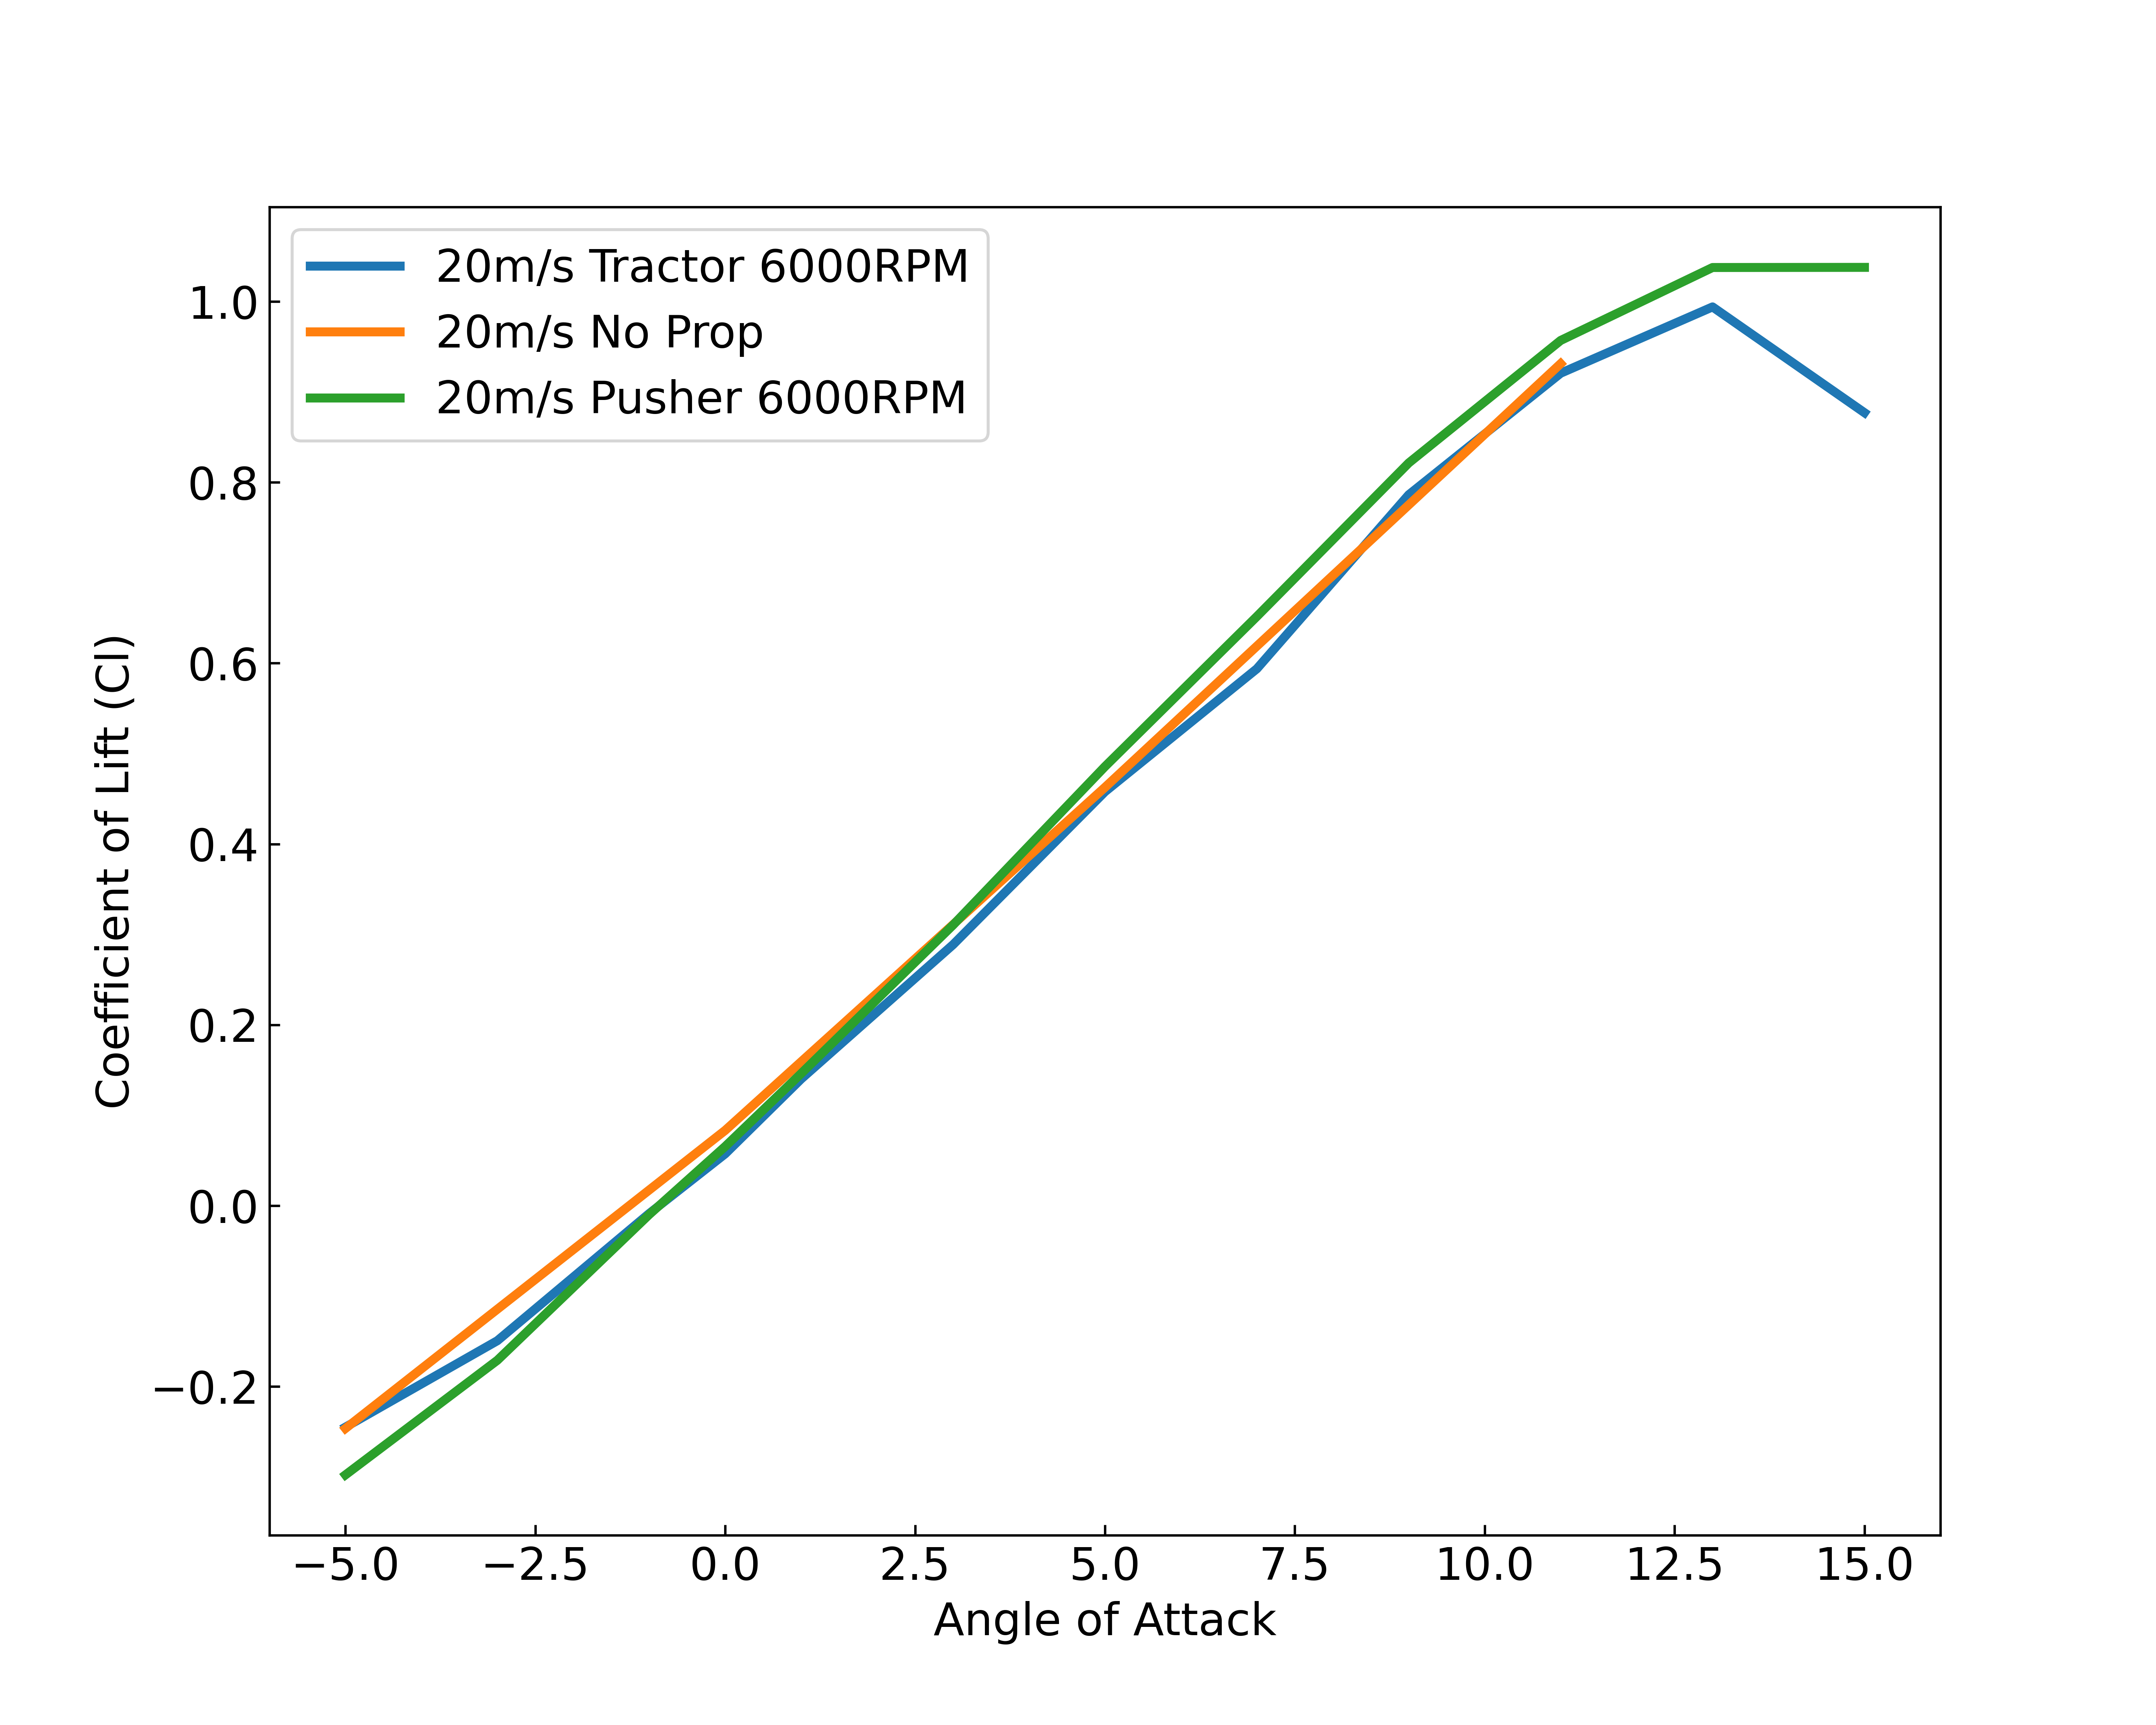
\includegraphics[width=\textwidth]{05_Results/Figs/Cl/20ms_6000RPM_Cl.png}
        \caption{Coefficient of lift at 20m/s airspeed and 6000RPM motor speed}
        \label{fig:Cl_20ms_6000}
    \end{subfigure}
    \begin{subfigure}[b]{0.467\textwidth}
        \centering
        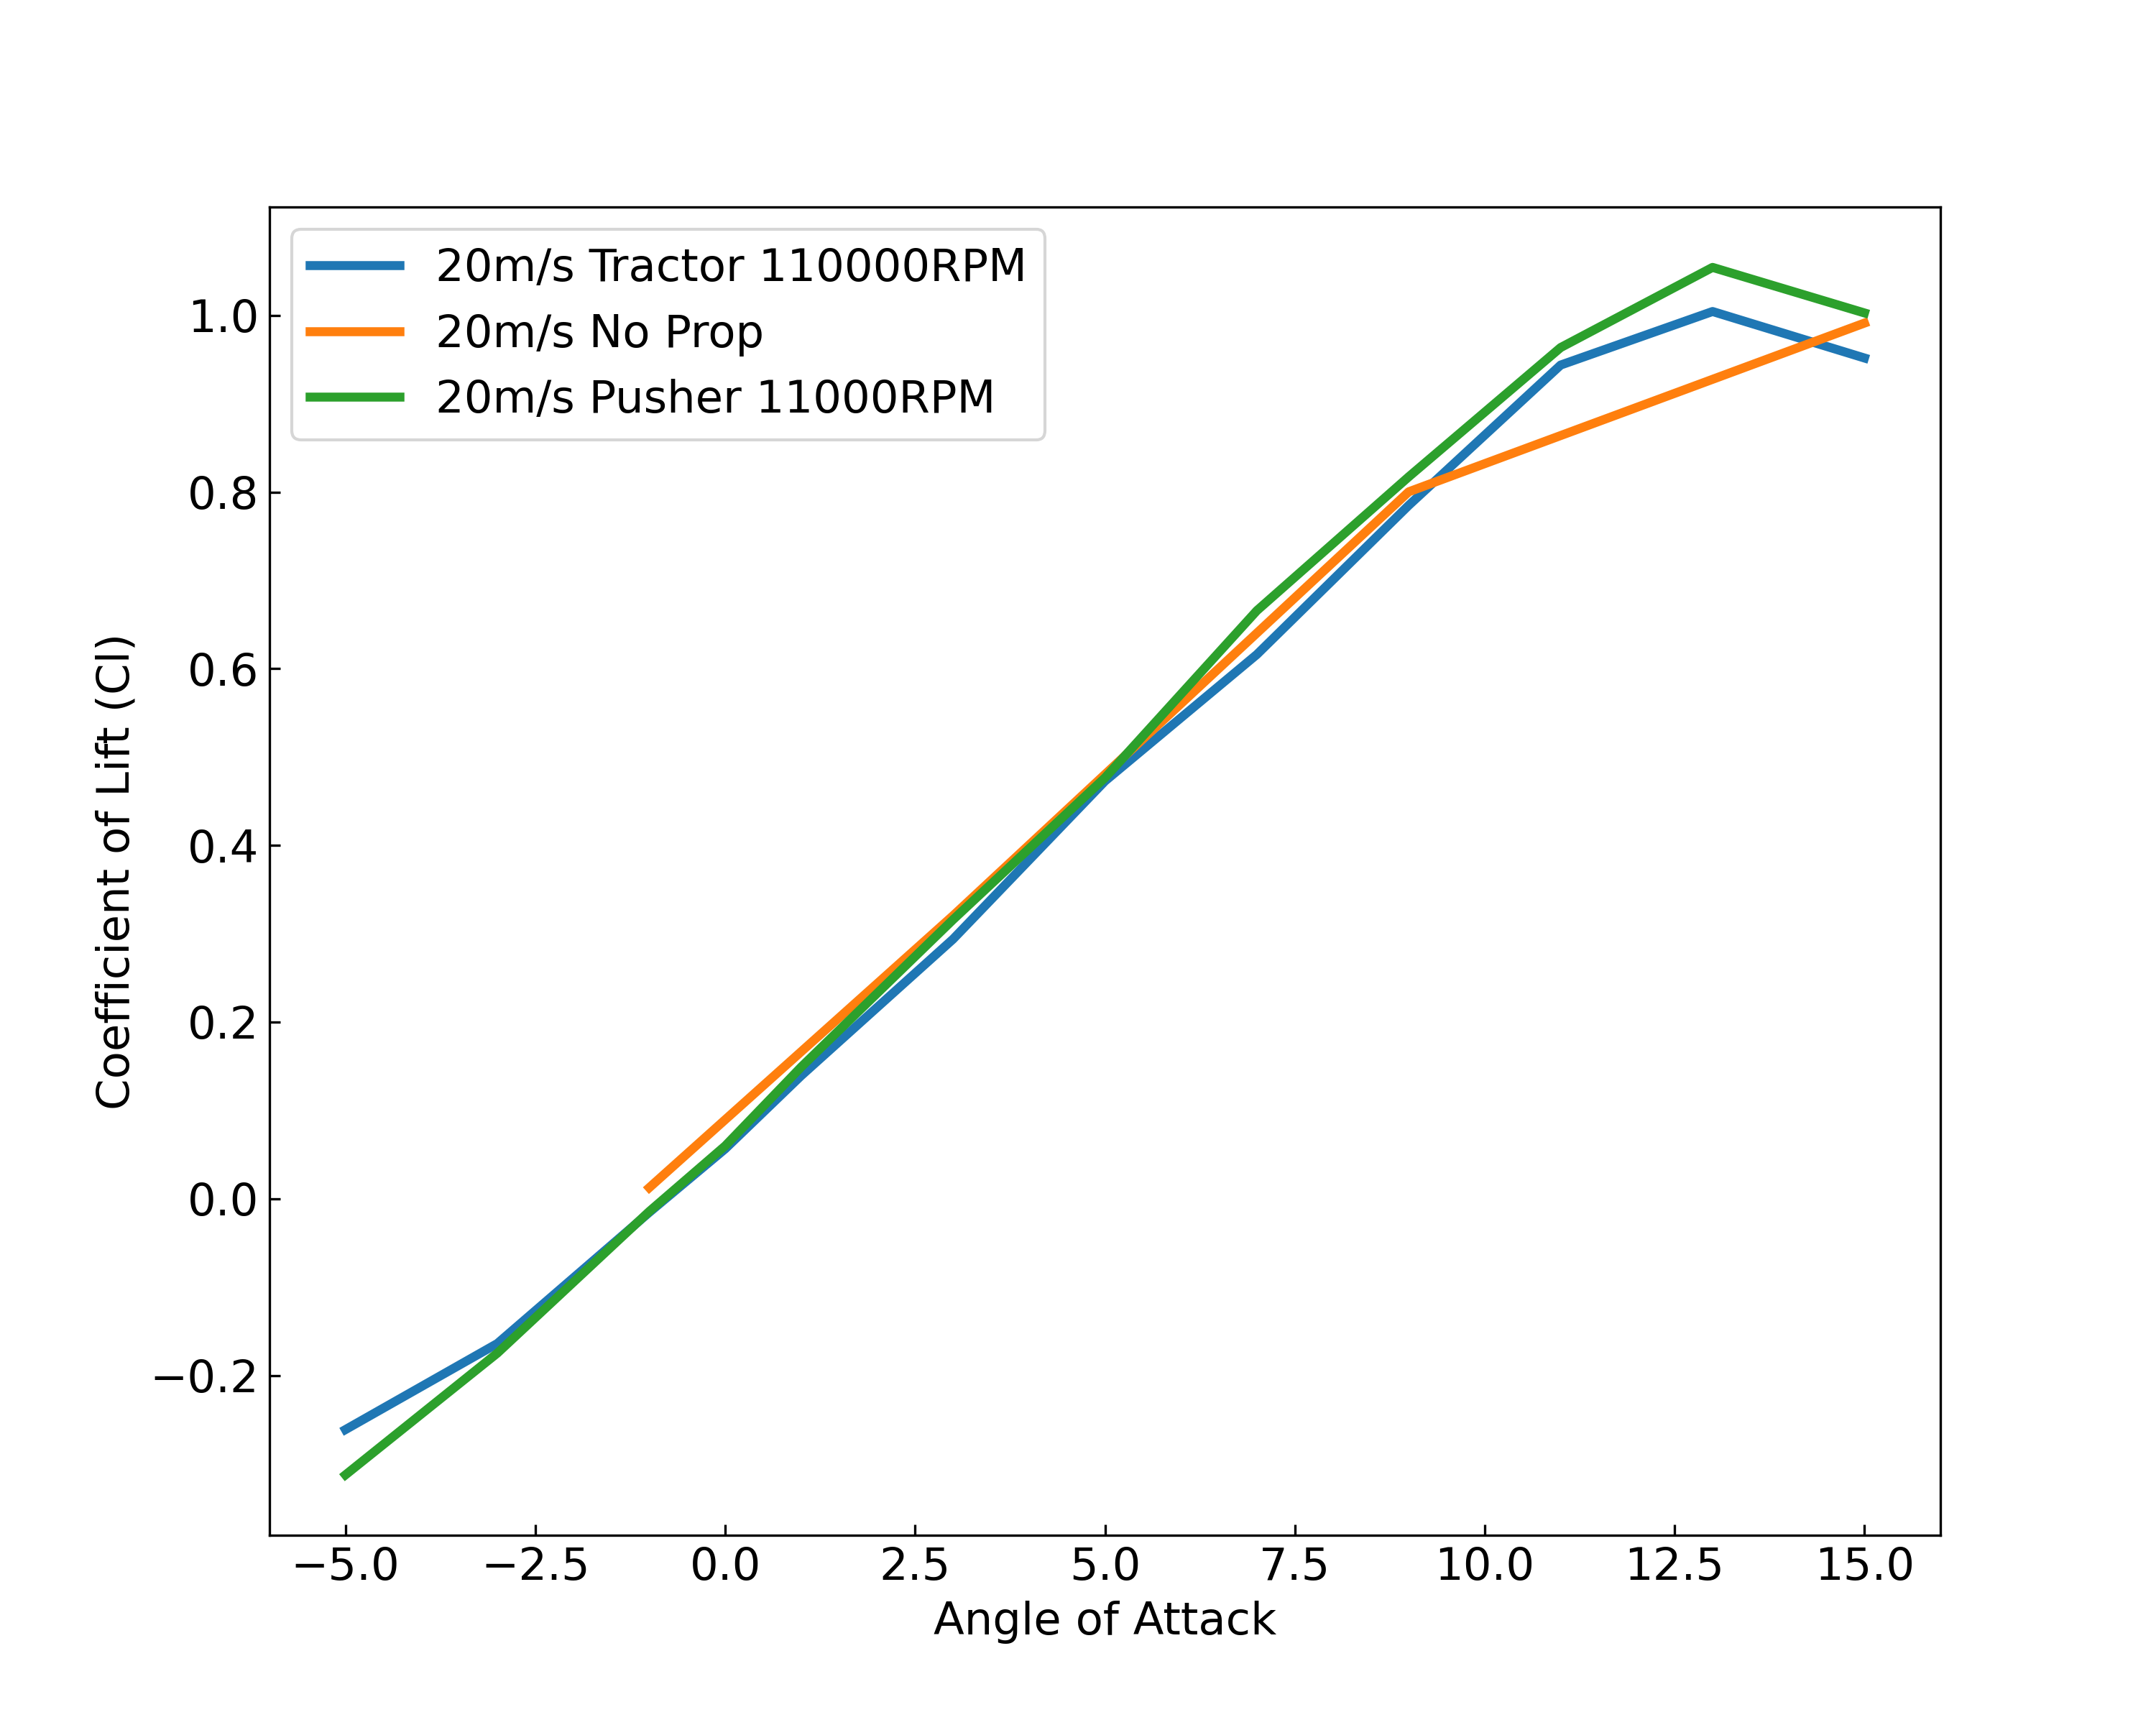
\includegraphics[width=\textwidth]{05_Results/Figs/Cl/20ms_110000RPM_Cl.png}
        \caption{Coefficient of lift at 20m/s airspeed and 11000RPM motor speed}
        \label{fig:Cl_20ms_11000}
    \end{subfigure}
    \caption{Coefficient of lift variation with various conditions for the pusher, tractor and no propeller configurations }
\end{figure}

\subsection{Aerodynamic Coefficient of Drag}
Figure \ref{fig:Cd_11000RPM} shows that as the wind tunnel airspeed increased, the drag coefficient shifted upwards for both the pusher and tractor configuration. The drag for both the tractor and puller configuration at 10m$s^{-1}$ airspeed is negative and shifts to positive value as the airspeed increases to 20m$s^{-1}$. This is due to the thrust produced by the propeller decreasing as the airspeed increases for both the tractor and puller configurations. The drag curve shifts into negative values for the tractor and puller configurations due to the thrust produced by the propeller. As the overall drag is a measure of the thrust minus drag, the overall drag becomes negative, shifting the coefficient of drag curve into negative values. As the airspeed increases, the drag coefficient is also seen to increase for the pusher and tractor configuration due to an increase in drag for the overall model with increasing airspeed. This shifts the coefficient of drag curves upwards as the airspeed increases. The highest drag coefficient occurred when no propeller operated on the MAV model. Ananda concluded that for tractor configuration propeller-wing set up in a low-speed wind tunnel, the flow transitions to turbulent flow earlier. This reduces the drag and increases the lift-to-drag ratio \cite{Ananda2018}. This shows a discrepancy with the results seen in this study. However, Ananda's setup involved a motor being mounted in front of the wing with no direct attachment; hence, the forces are not directly applied to the wing \cite{Ananda2018}. When no propeller is added, no significant changes are seen in airspeed for the drag coefficient. The tractor configuration, in general, produces less drag than the pusher configuration; hence, the drag coefficient is lower for the tractor configuration. This is most clearly seen at 20m$s^{-1}$ in Figure \ref{fig:Cd_11000RPM}. 




\begin{figure}[H]
    \centering
    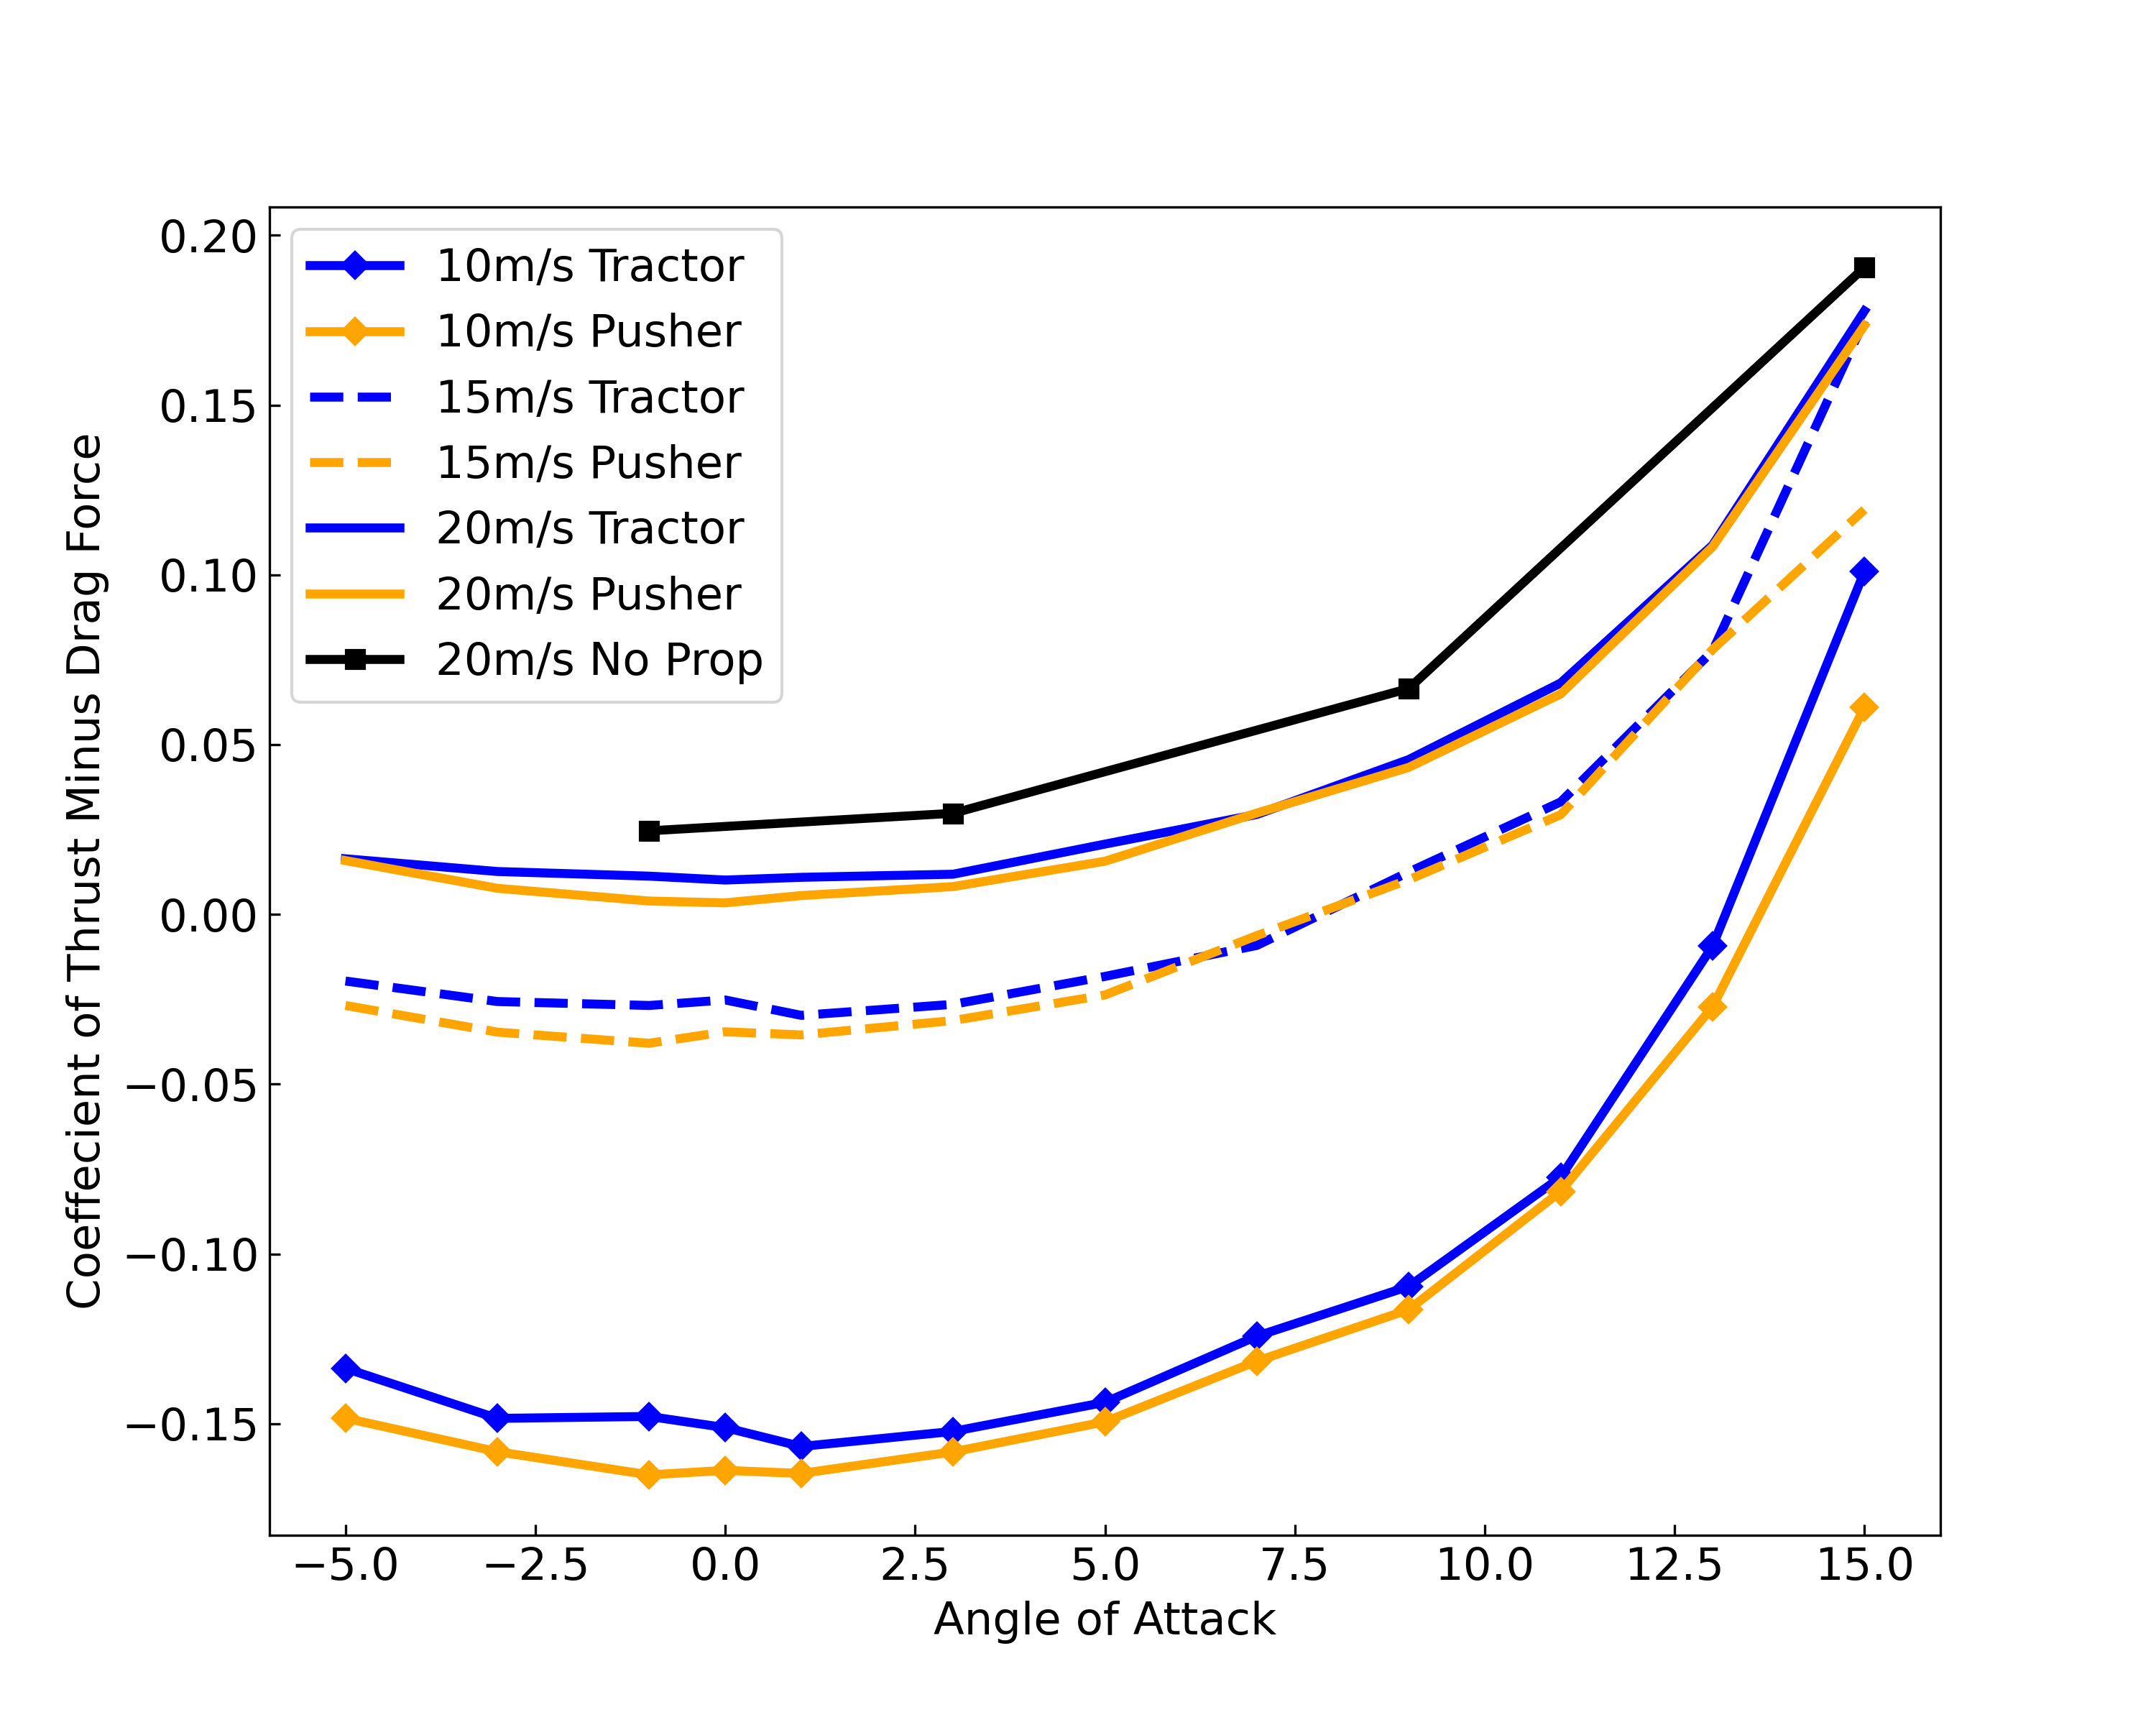
\includegraphics[scale = 0.7]{05_Results/Figs/Cd/110000RPM_Cd.png}
    \caption{Coefficient of drag variation at 11000RPM motor speed for the tractor, pusher and no propeller configurations}
    \label{fig:Cd_11000RPM}
\end{figure}

Figure \ref{fig:Cd_20ms} shows minimal differences between the pusher and tractor configurations. The addition of the propeller increases the drag coefficient at 6000RPM and shows that the propellers do not produce enough thrust to overcome the drag at 20m$s^{-1}$. As the motor speed increases to 11000RPM, there is a significant drop in the drag coefficient for both the tractor and pusher configuration, showing that the thrust produced can overcome drag at 11000RPM. 


\begin{figure}[H]
    \centering
    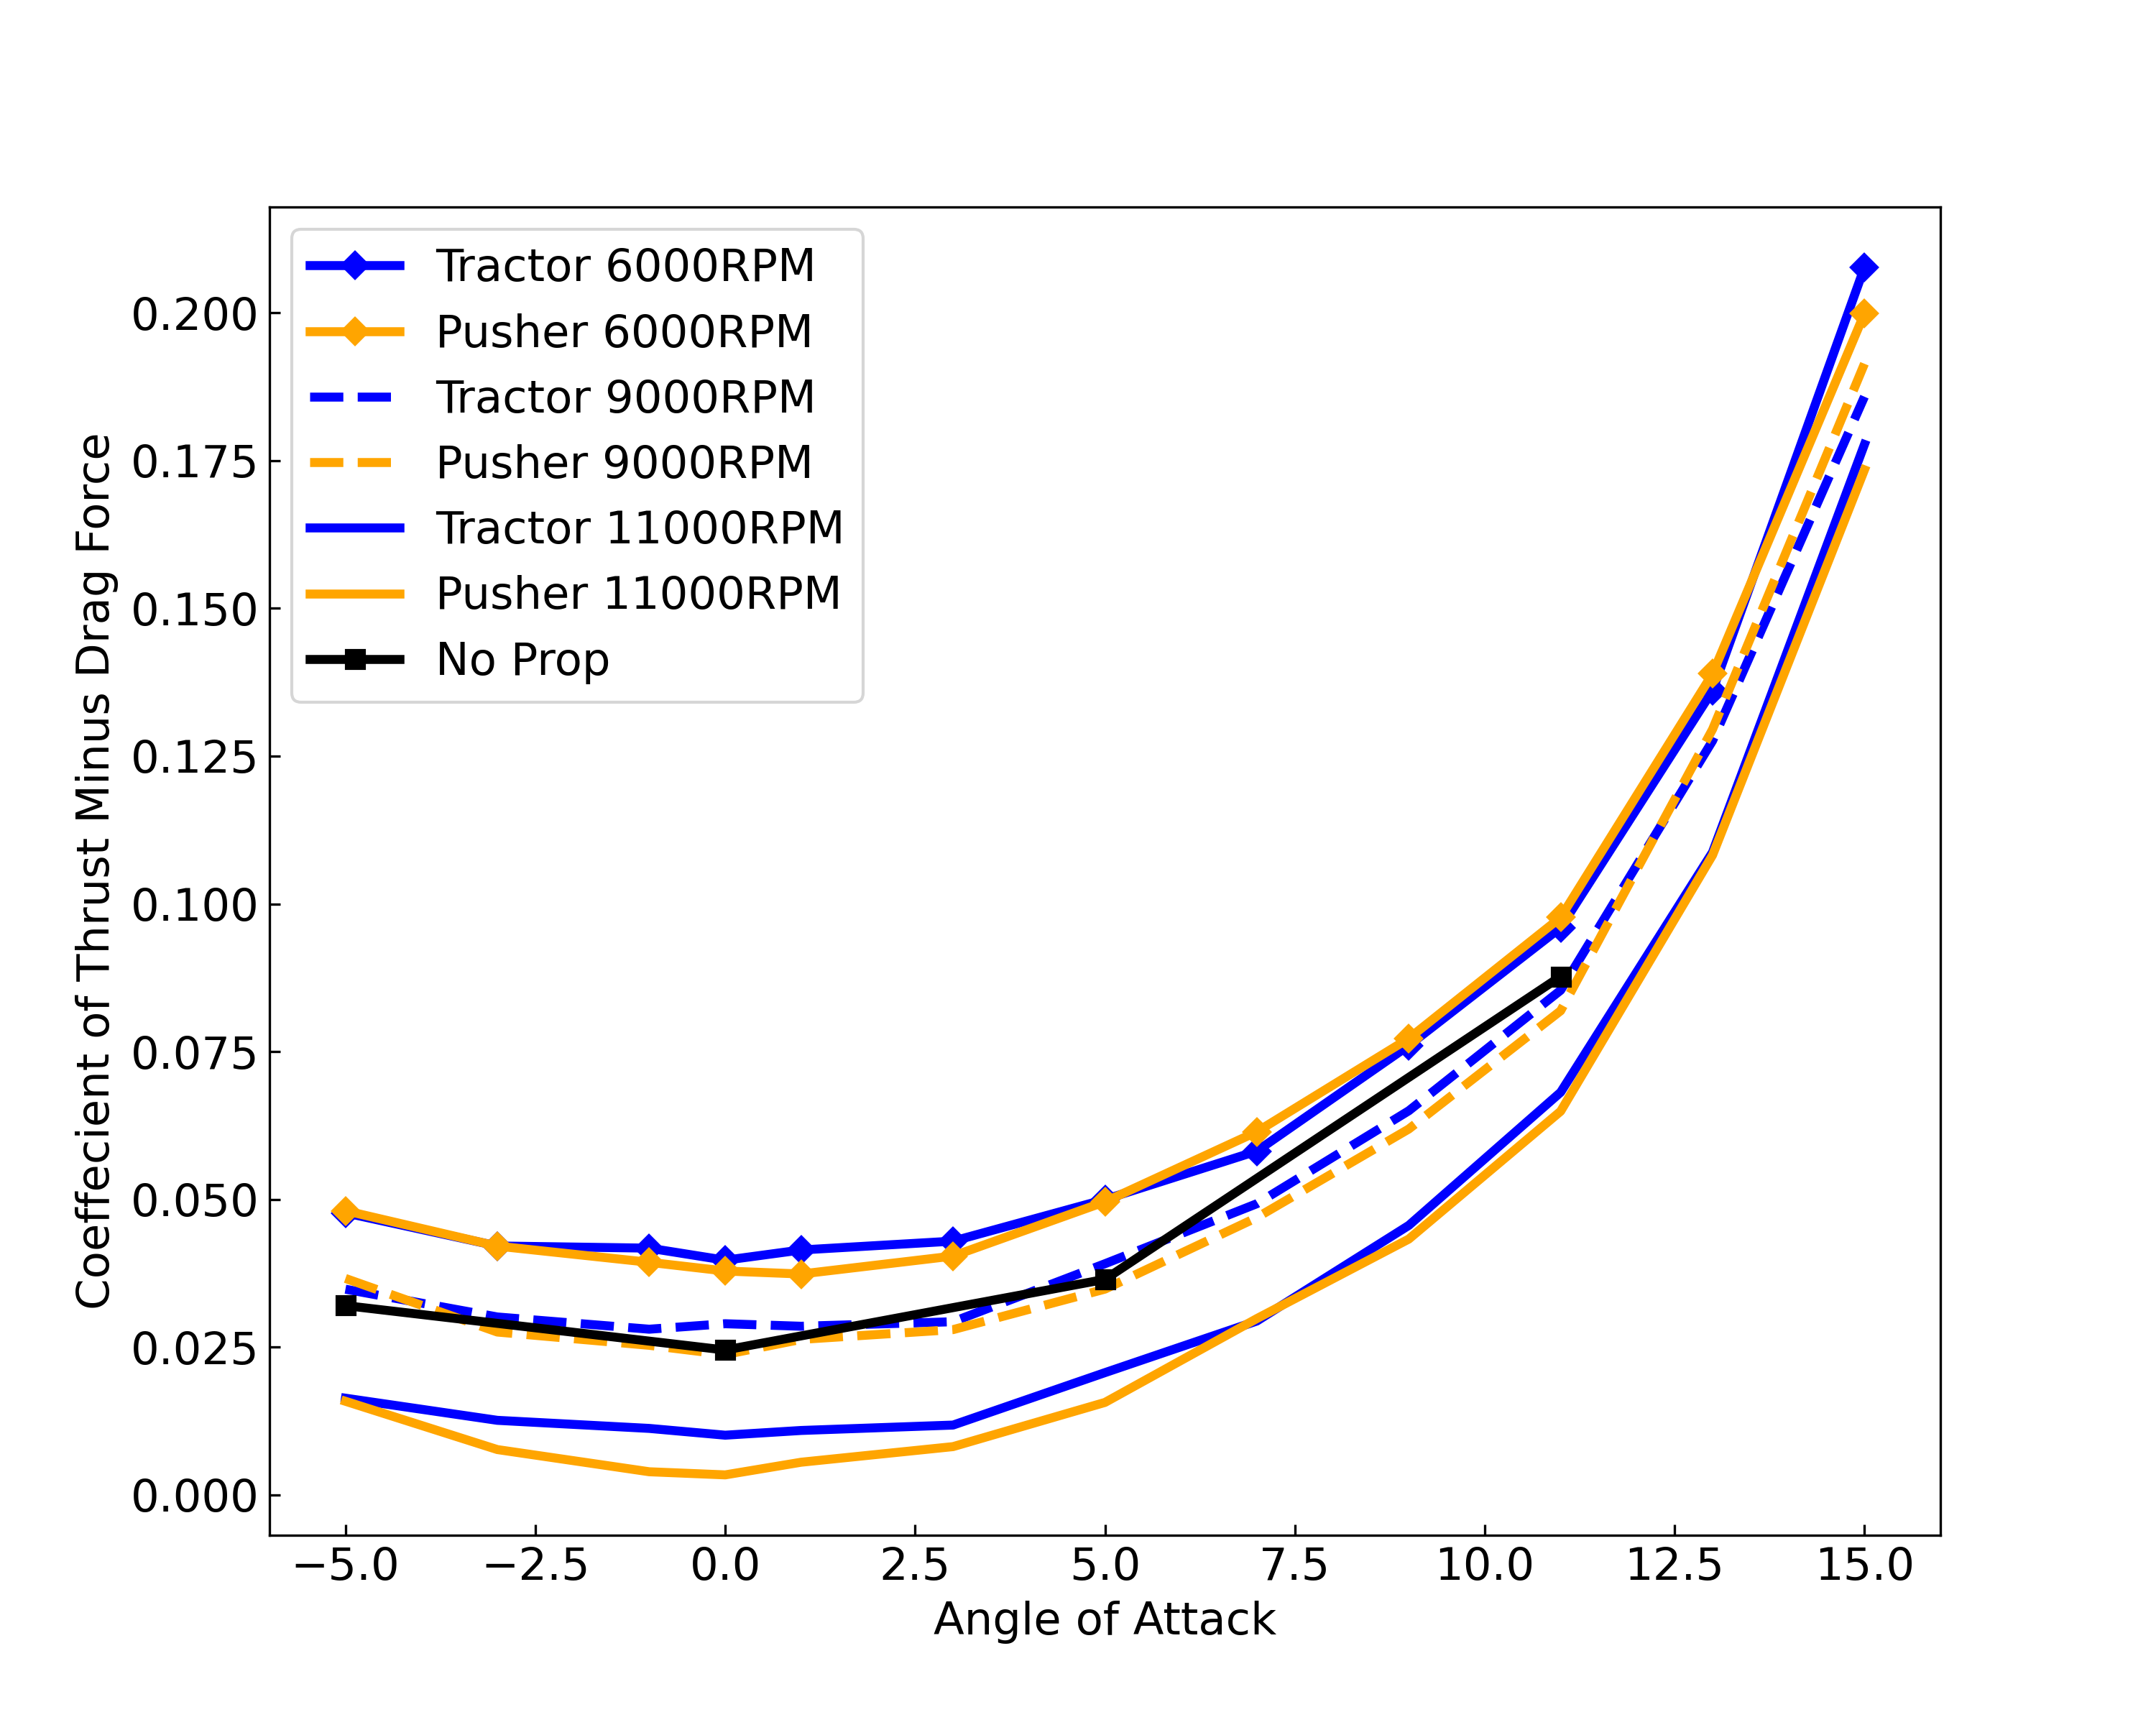
\includegraphics[scale = 0.7]{05_Results/Figs/Cd/20ms_Cd.png}
    \caption{Coefficient of drag variation at 20ms airspeed for the tractor, pusher and no propeller configuration}
    \label{fig:Cd_20ms}
\end{figure}



\subsection{Pitching Moment Coefficient}

Figures \Cref{fig:Cm_10ms_6000} to \Cref{fig:Cm_20ms_11000} show that for all cases, the pitching moment of the MAV model decreases as the angle of attack increases. This leads to a stable MAV in all cases as the longitudinal stability is maintained due to the pitching down motion of the MAV as the \acrshort{AoA} increases. Figures \Cref{fig:Cm_10ms_6000} to \Cref{fig:Cm_20ms_11000} also show that as the motor speed increases from 6000RPM to 11000RPM, the tractor configuration experienced a decrease in pitching coefficient compared with the no propeller model up until stall at approximately 12$^\circ$ AoA. The pusher configuration experienced an increase in the pitching moment compared with the no-propeller model. This shows that as the airspeed and propeller speed increase, the tractor configuration becomes less stable, while the pusher configuration becomes more stable. Increasing the airspeed decreased the pitching moment for all motor speeds.

\begin{figure}[H]
    \centering
    \begin{subfigure}[b]{0.467\textwidth}
        \centering
        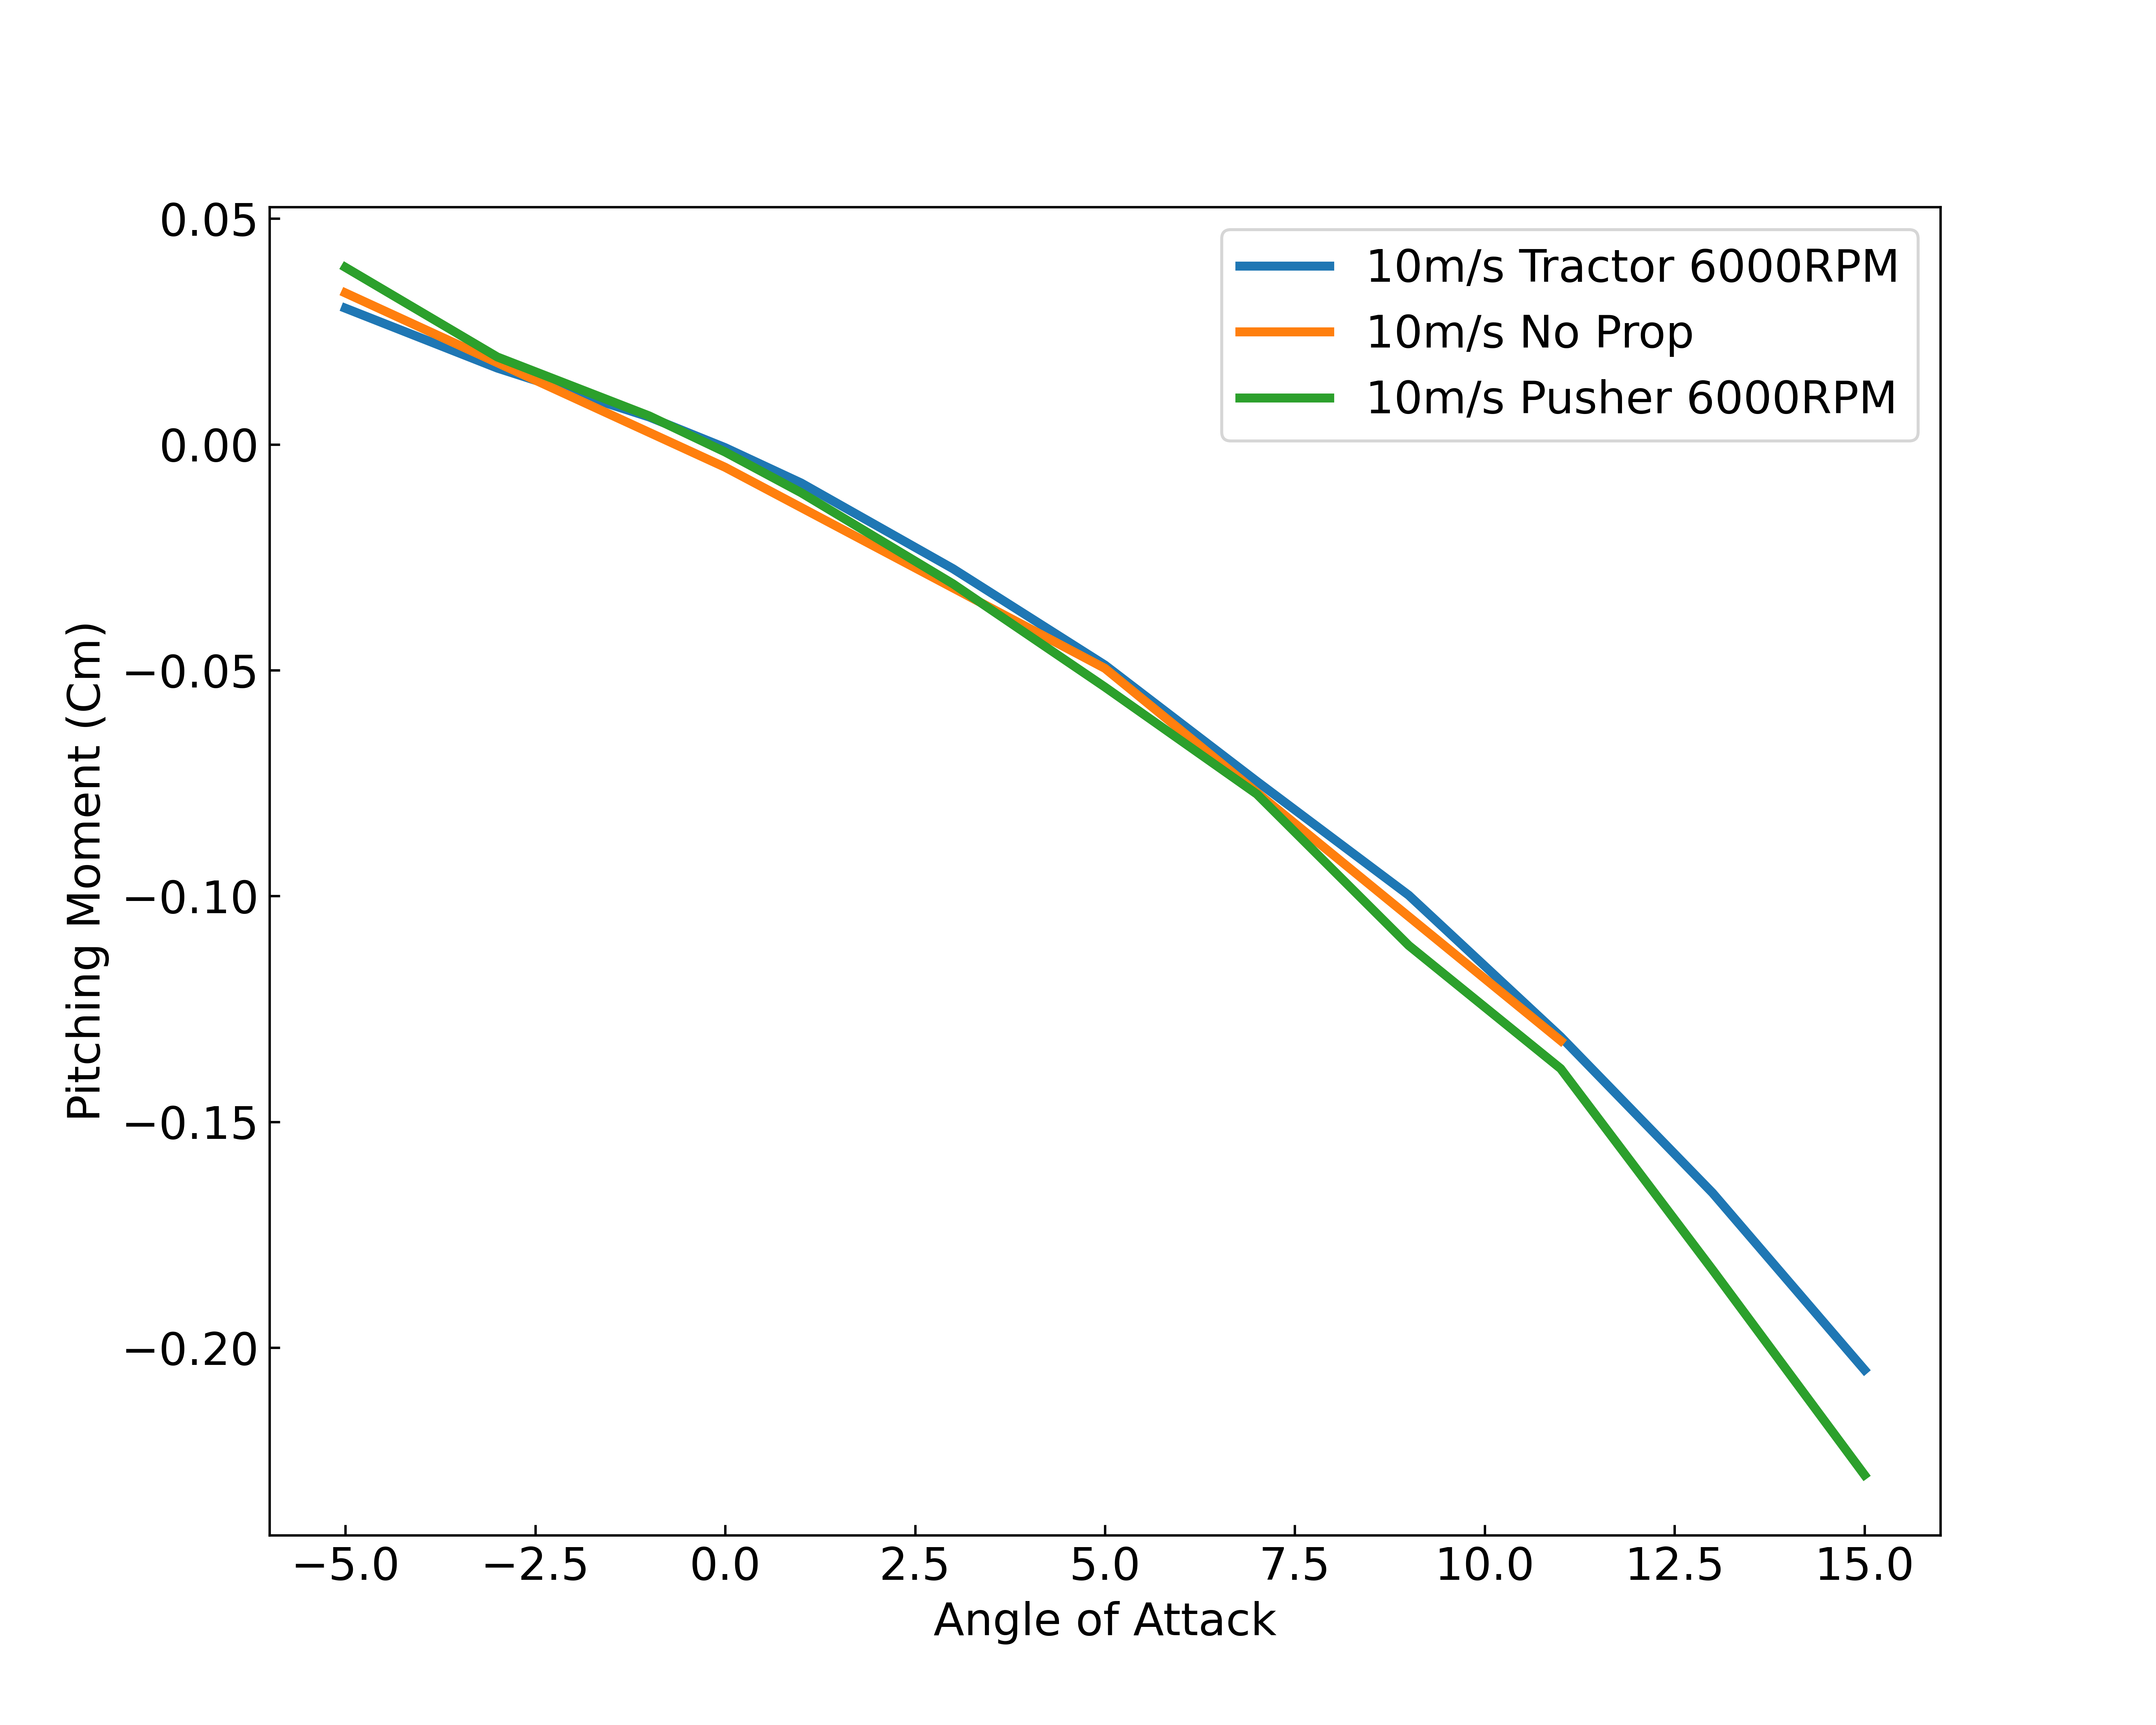
\includegraphics[width=\textwidth]{05_Results/Figs/Cm/10ms_6000RPM_Cm.png}
        \caption{Pitching Moment Coefficient at 10m/s airspeed and 6000RPM motor speed}
        \label{fig:Cm_10ms_6000}
    \end{subfigure}
    \begin{subfigure}[b]{0.467\textwidth}
        \centering
        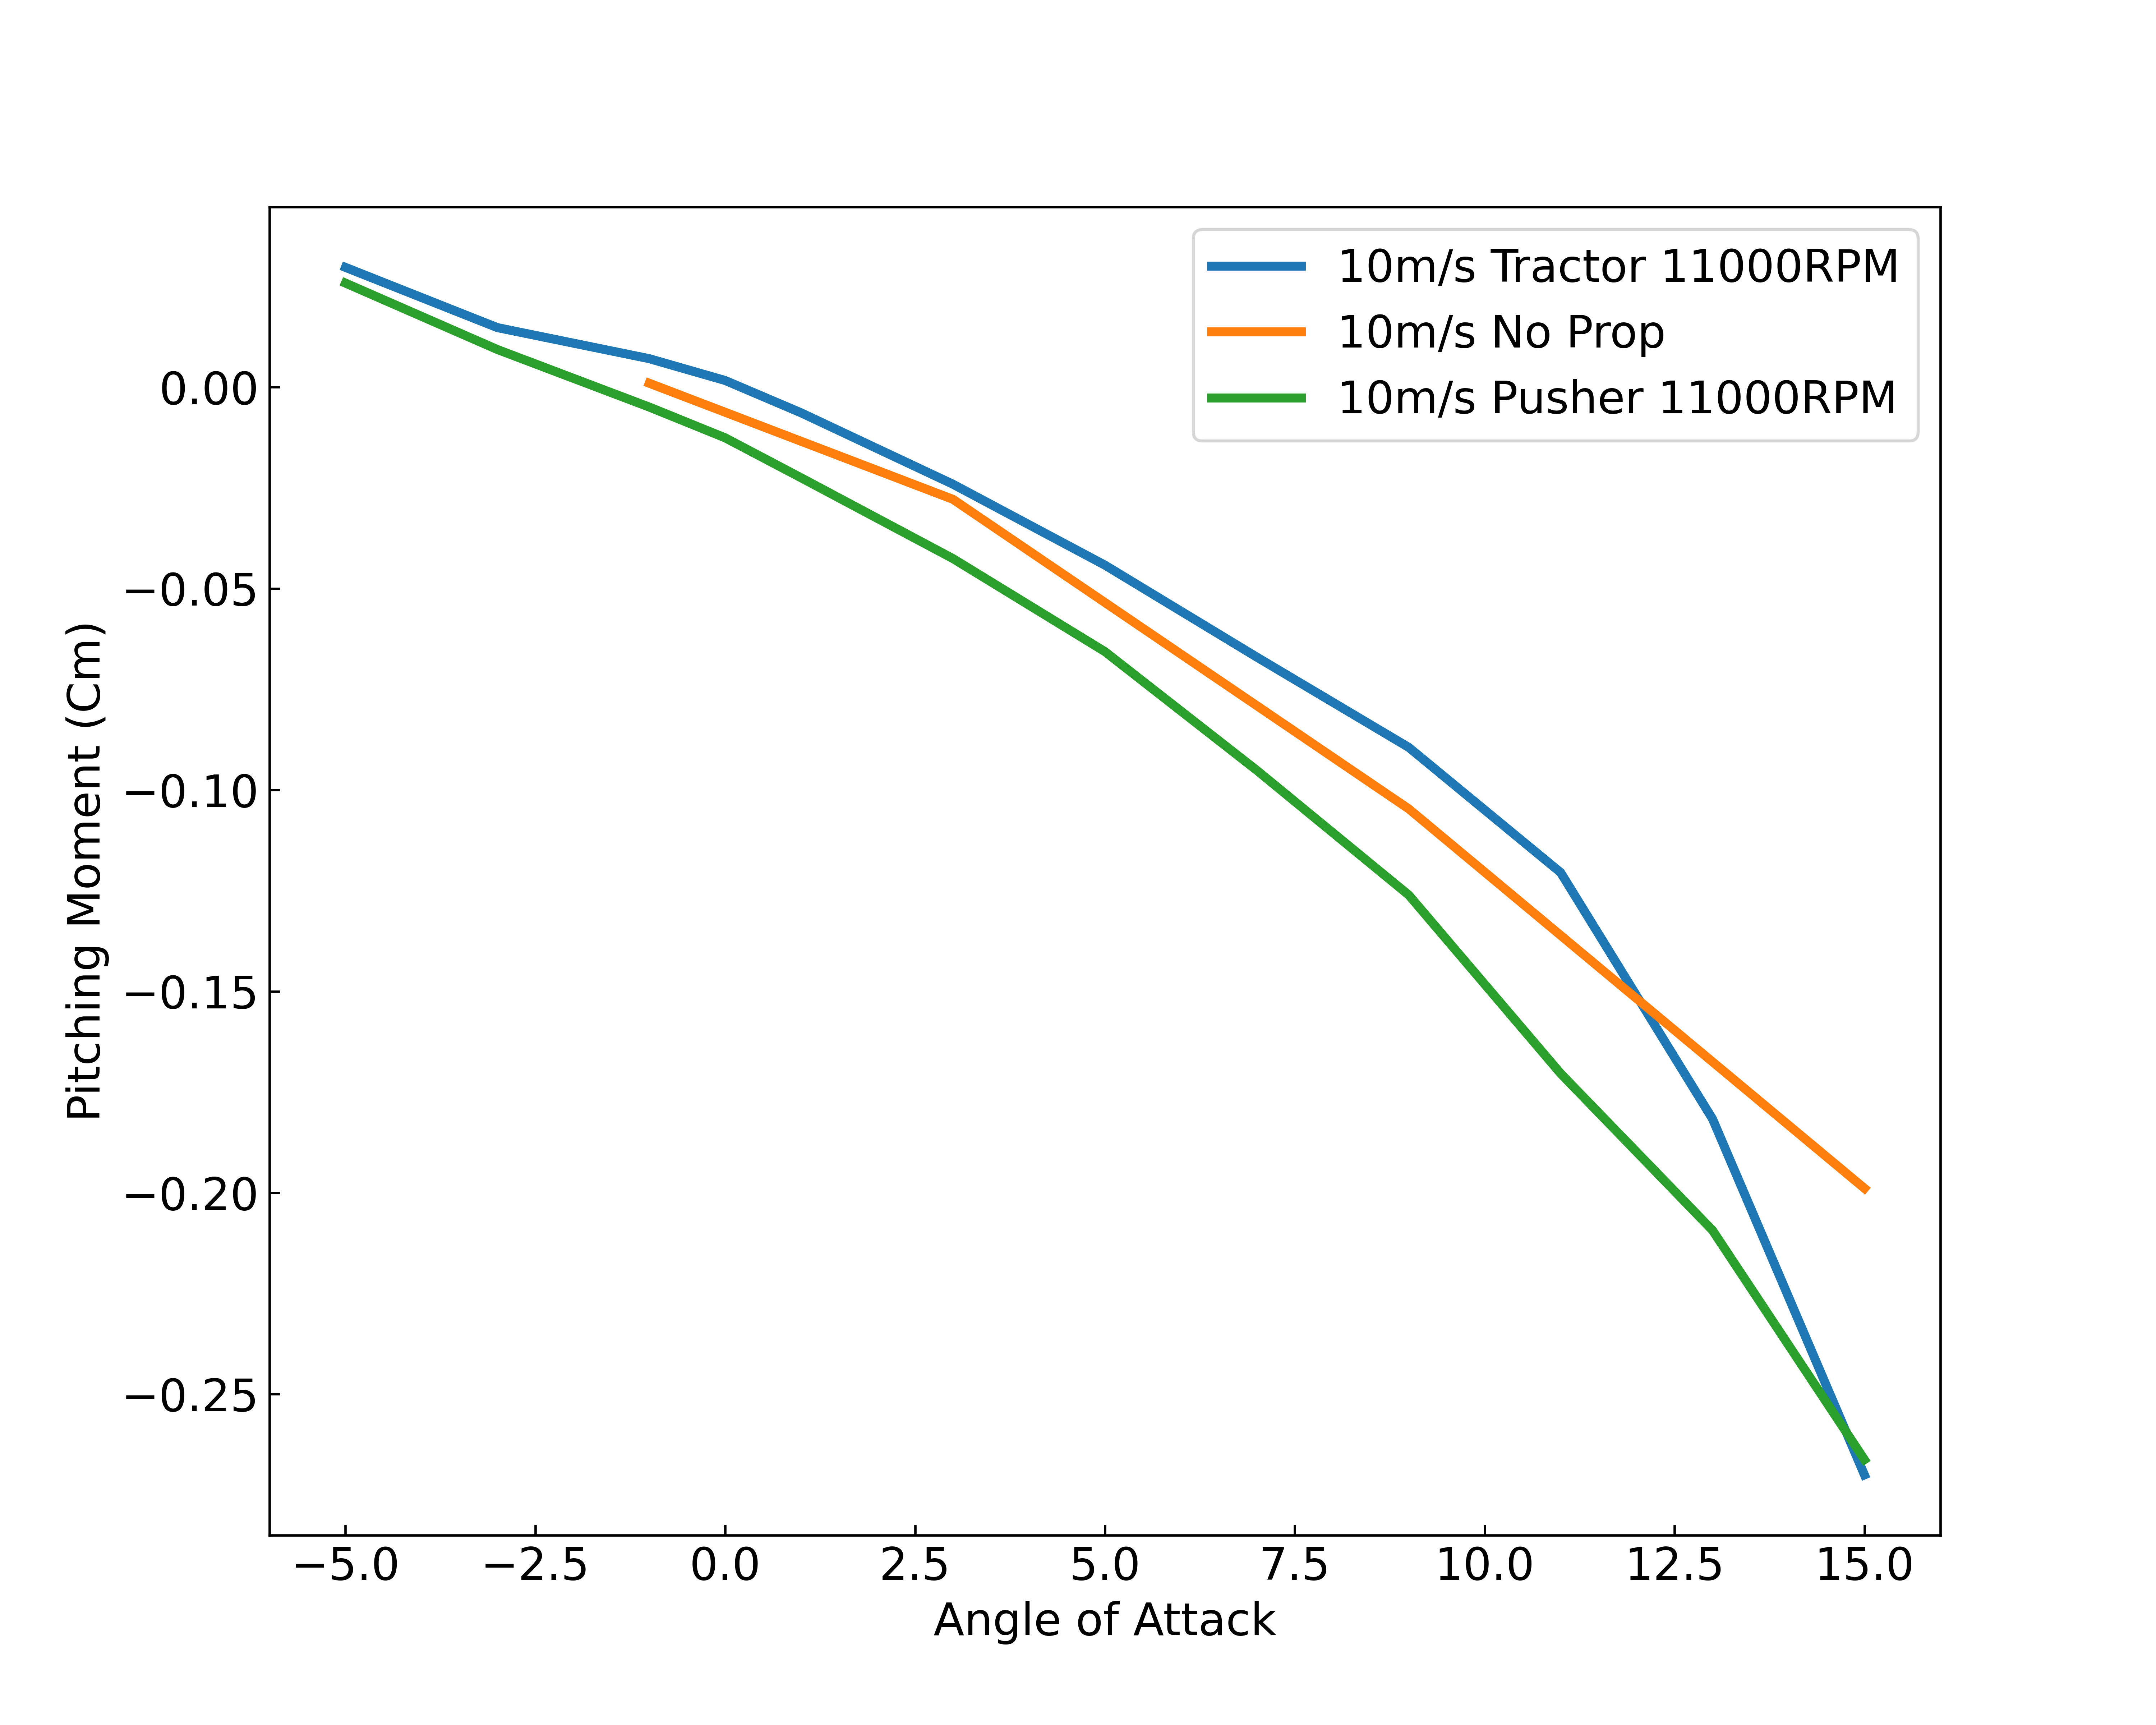
\includegraphics[width=\textwidth]{05_Results/Figs/Cm/10ms_11000RPM_Cm.png}
        \caption{Pitching Moment Coefficient at 10m/s airspeed and 11000RPM motor speed}
        \label{fig:Cm_10ms_11000}
    \end{subfigure}
    \begin{subfigure}[b]{0.467\textwidth}
        \centering
        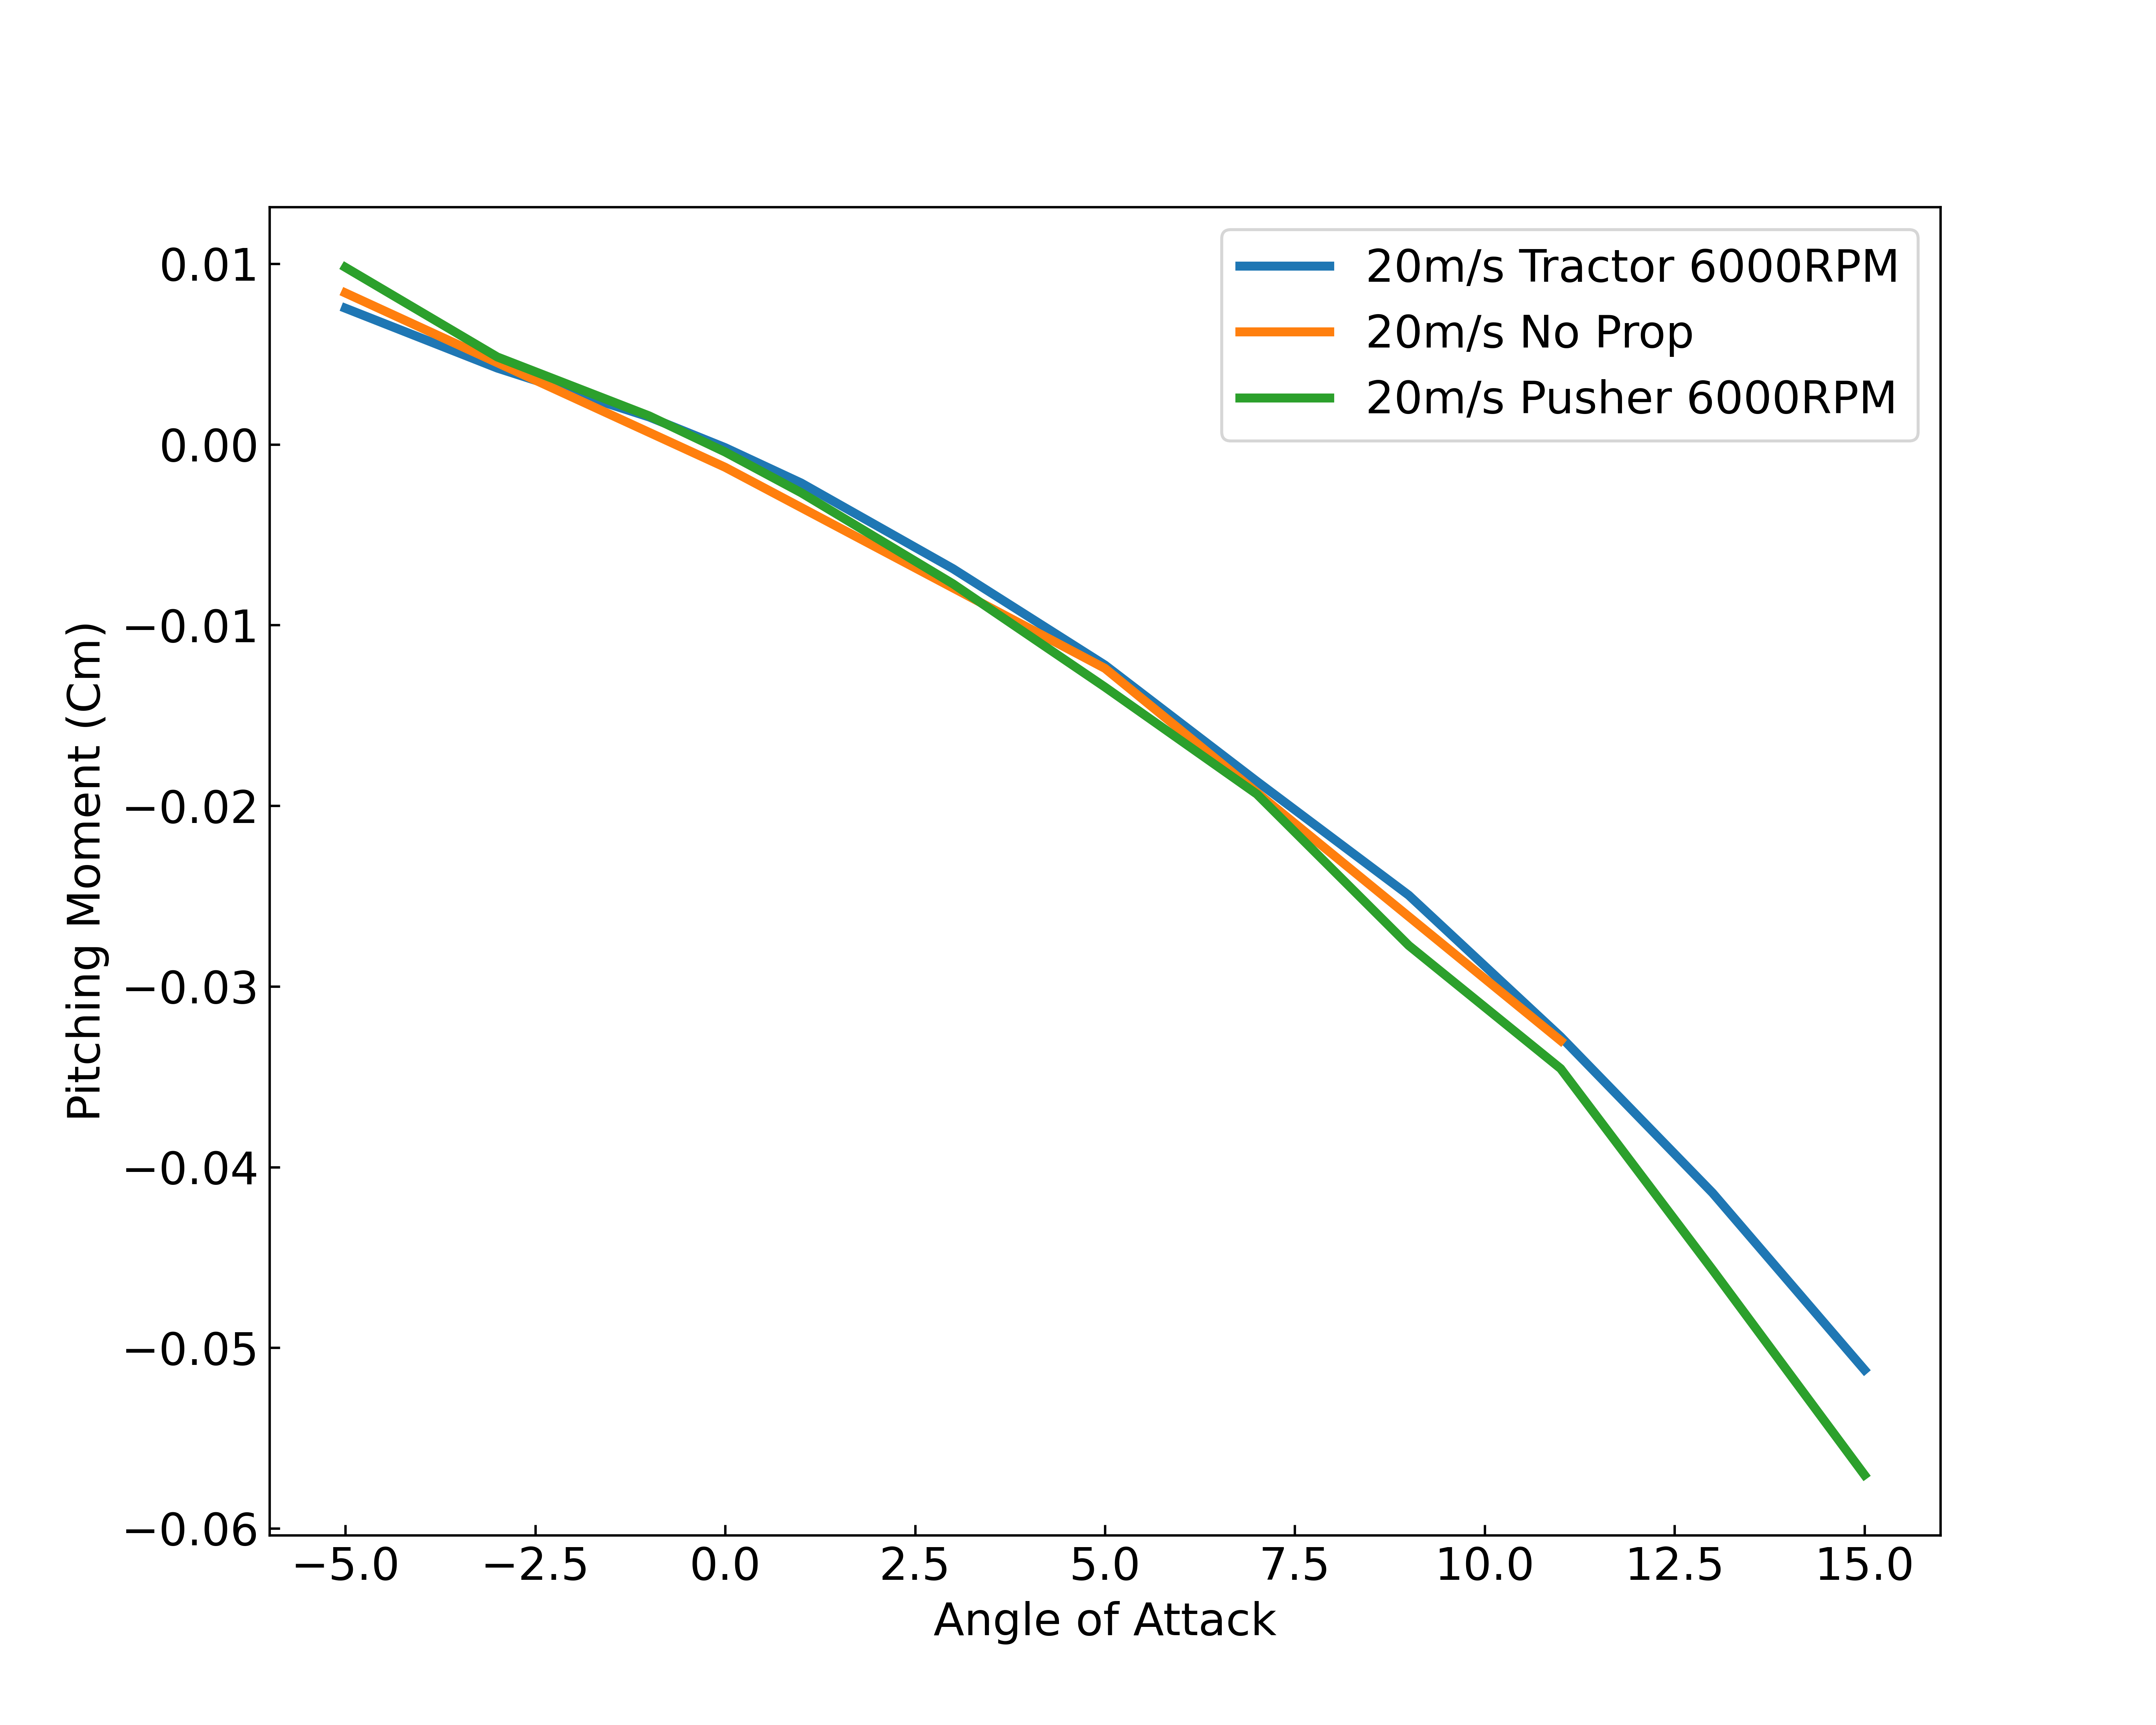
\includegraphics[width=\textwidth]{05_Results/Figs/Cm/20ms_6000RPM_Cm.png}
        \caption{Pitching Moment Coefficient at 20m/s airspeed and 6000RPM motor speed}
        \label{fig:Cm_20ms_6000}
    \end{subfigure}
    \begin{subfigure}[b]{0.467\textwidth}
        \centering
        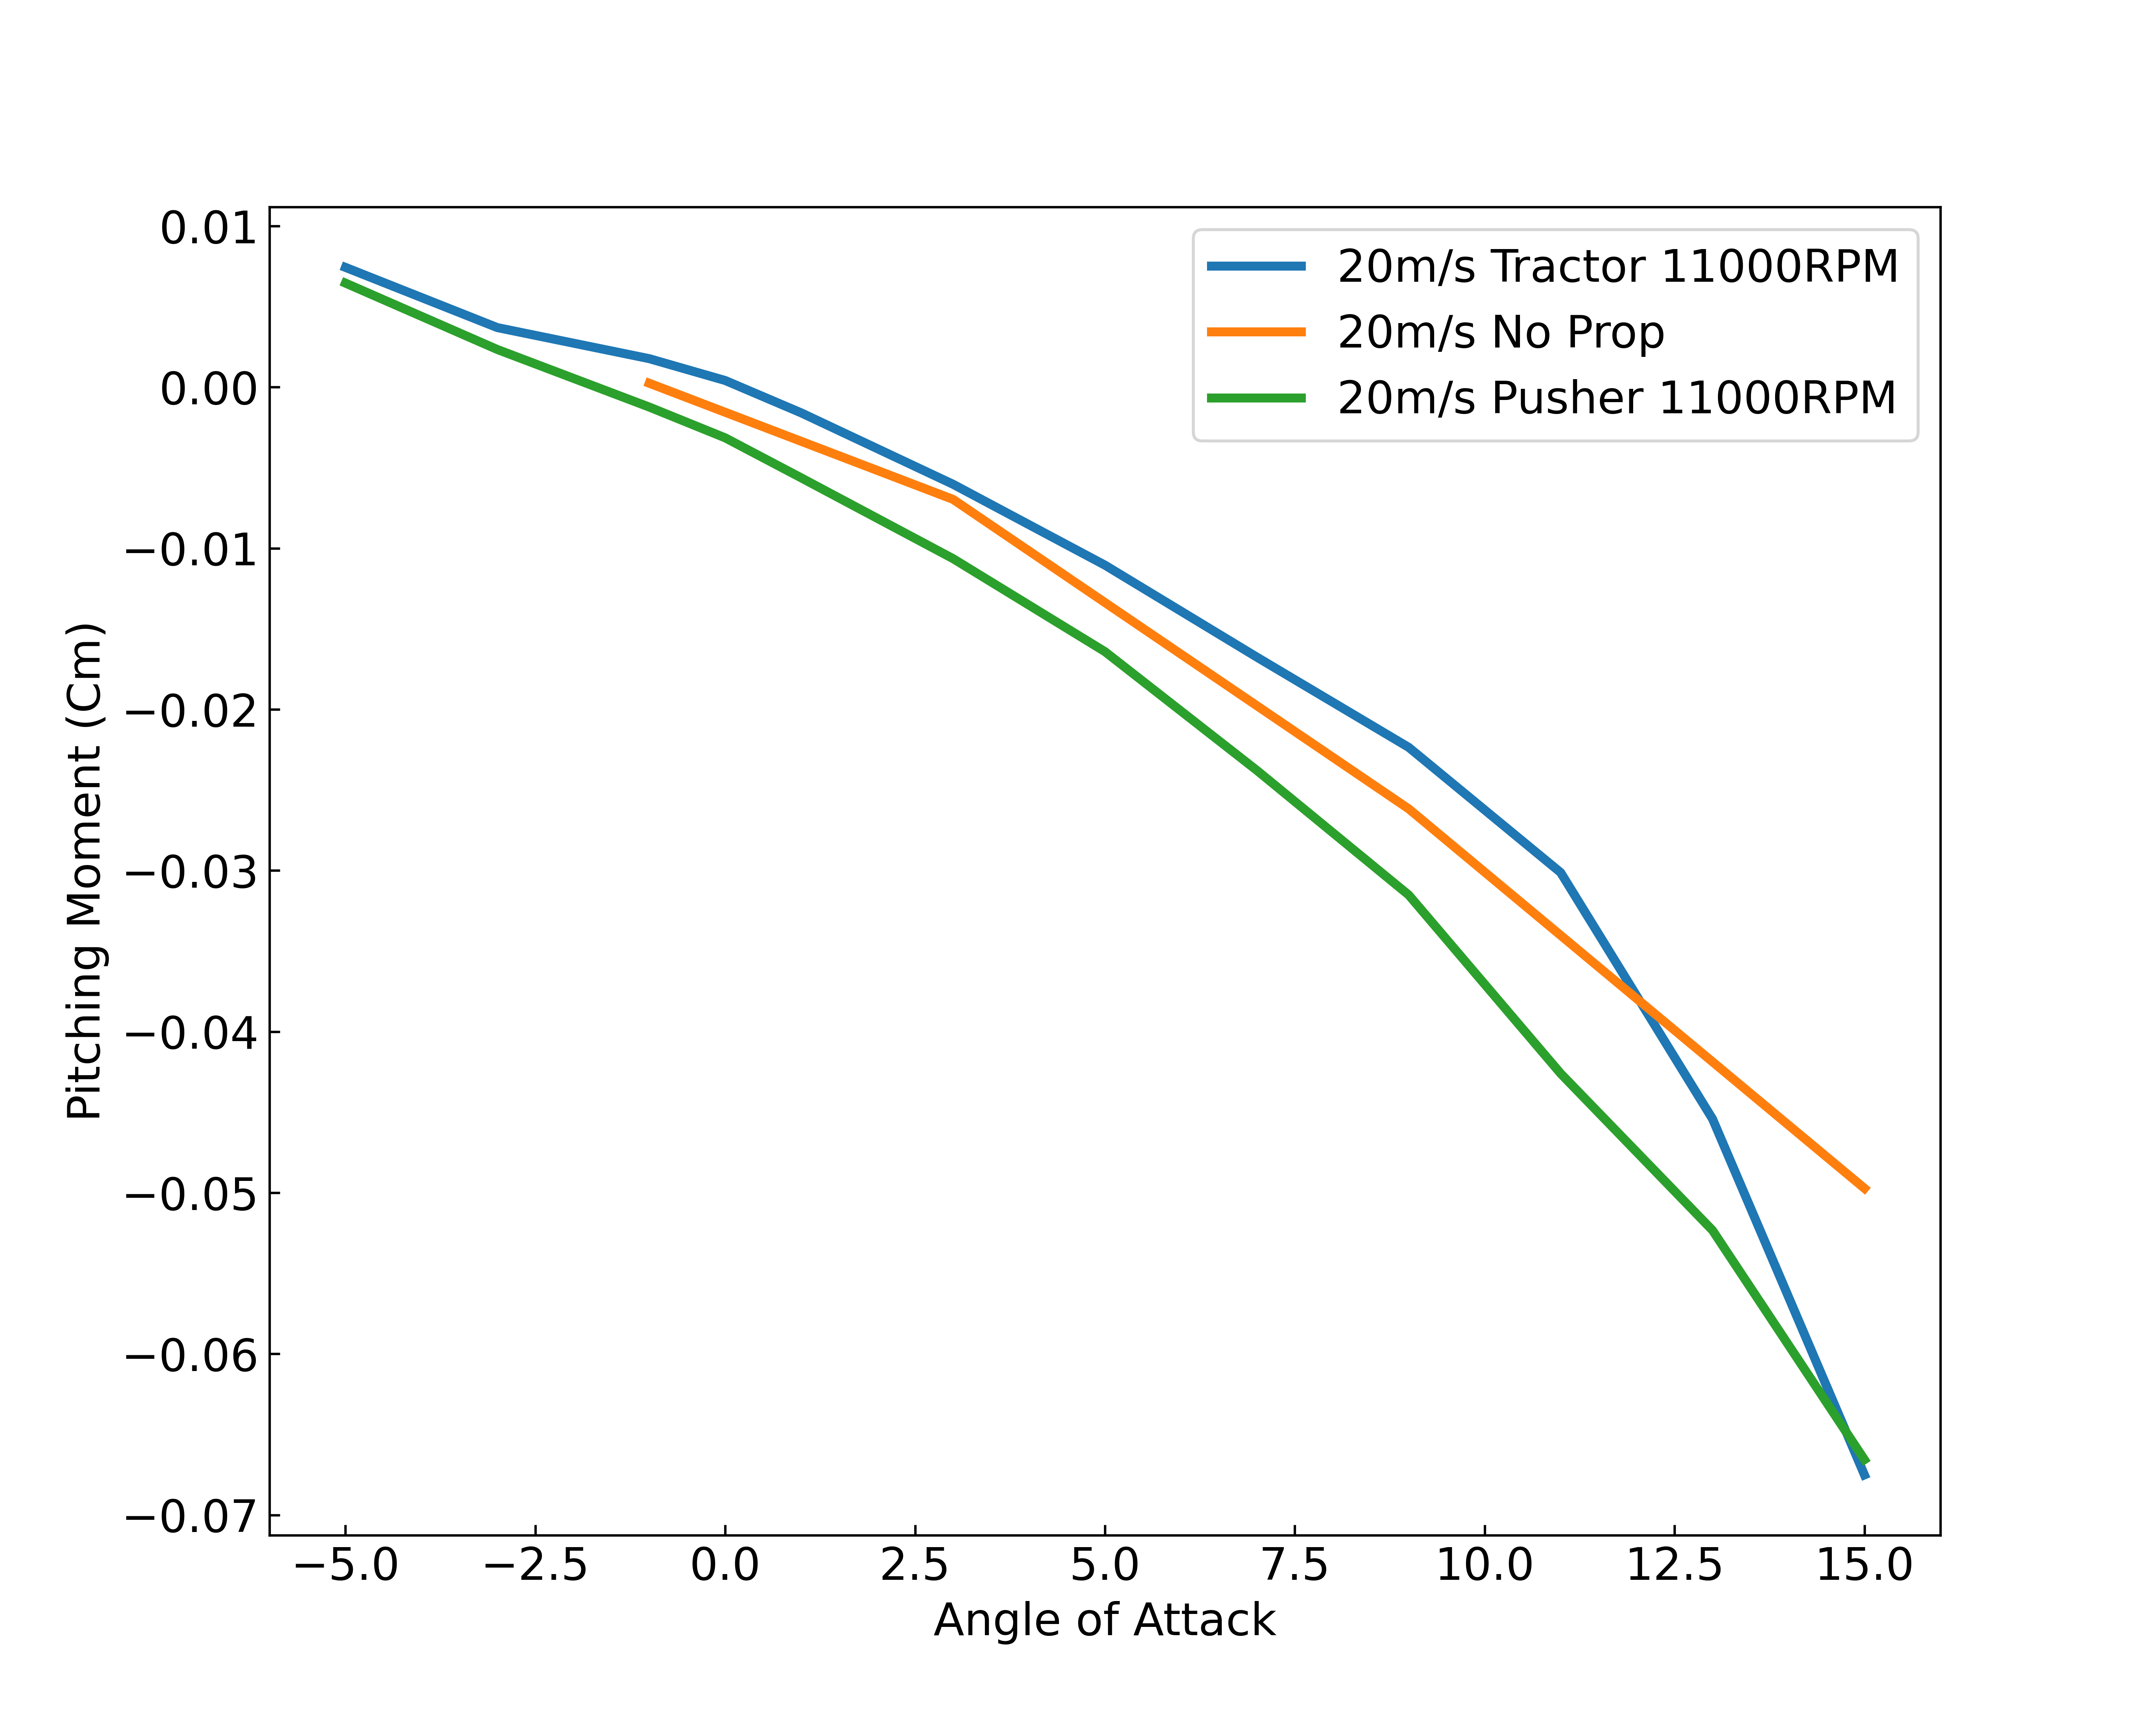
\includegraphics[width=\textwidth]{05_Results/Figs/Cm/20ms_11000RPM_Cm.png}
        \caption{Pitching Moment Coefficient at 20m/s airspeed and 11000RPM motor speed}
        \label{fig:Cm_20ms_11000}
    \end{subfigure}
    
\end{figure}

\subsection{Rolling Moment Coefficient}

The rolling coefficient for the tractor configuration when the propeller is run at 6000RPM was shifted downwards compared to both the pusher and no propeller configurations, leading to a decrease in the rolling moment for all speeds. When the propeller speed increased to 11000RPM, the tractor configuration did not show a significant shift downwards until a sharp drop, seen at $\approx$12.5$^{\circ}$ \acrshort{AoA}. However, the pusher configuration shows a shift upwards and an increase in the rolling coefficient for all airspeeds and propeller speeds. The rolling moment is largely due to the propeller torque effect in which an asymmetric roll is produced due to the propeller wing interaction, previously described in Section \ref{sec:propellerWingInteraction}. The tractor configuration also experiences a flow distribution change over the wings and fuselage due to the propeller's upwash and downwash effect, as described in Section \ref{sec:propellerWingInteraction}. These propeller effects affect the lift distribution across the wings' surface, shifting the roll moment coefficient upwards as one wing is in the upwash of the propeller blades and the other in the downwash airstream. As the angle of attack increases, this rolling moment increases until sharply dropping off in Figures \Cref{fig:Cl_roll_10ms_6000} to \Cref{fig:Cl_roll_20ms_11000} as the right wing of the MAV stalled first, creating a lift force imbalance as the left wing continues to produce a lift force. At the same time, the right-wing experiences flow separation due to stalling. The rolling moment Sharply raises as the left wing also stalls and the flow over the left wing separates. The pusher configuration shifts the rolling moment to a larger extent due to having a larger moment arm from the position of the propeller to the aerodynamic centre of the MAV model than the tractor configuration. The pusher configuration also shows a bump at 0$^{\circ}$ \acrshort{AoA} for all airspeeds, while the tractor configuration shows this only when the propeller is running at 11000RPM. The rolling moment also decreases after 2.5$^{\circ}$ \acrshort{AoA} for the tractor configuration when the propeller runs at 11000RPM. \todo{explaination??} The increases in roll moment at 0$^{\circ}$ \acrshort{AoA} is likely due to an interaction with the wing and/or the wings wake. However, more investigation needs to validate this.  

\begin{figure}[H]
    \centering
    \begin{subfigure}[b]{0.467\textwidth}
        \centering
        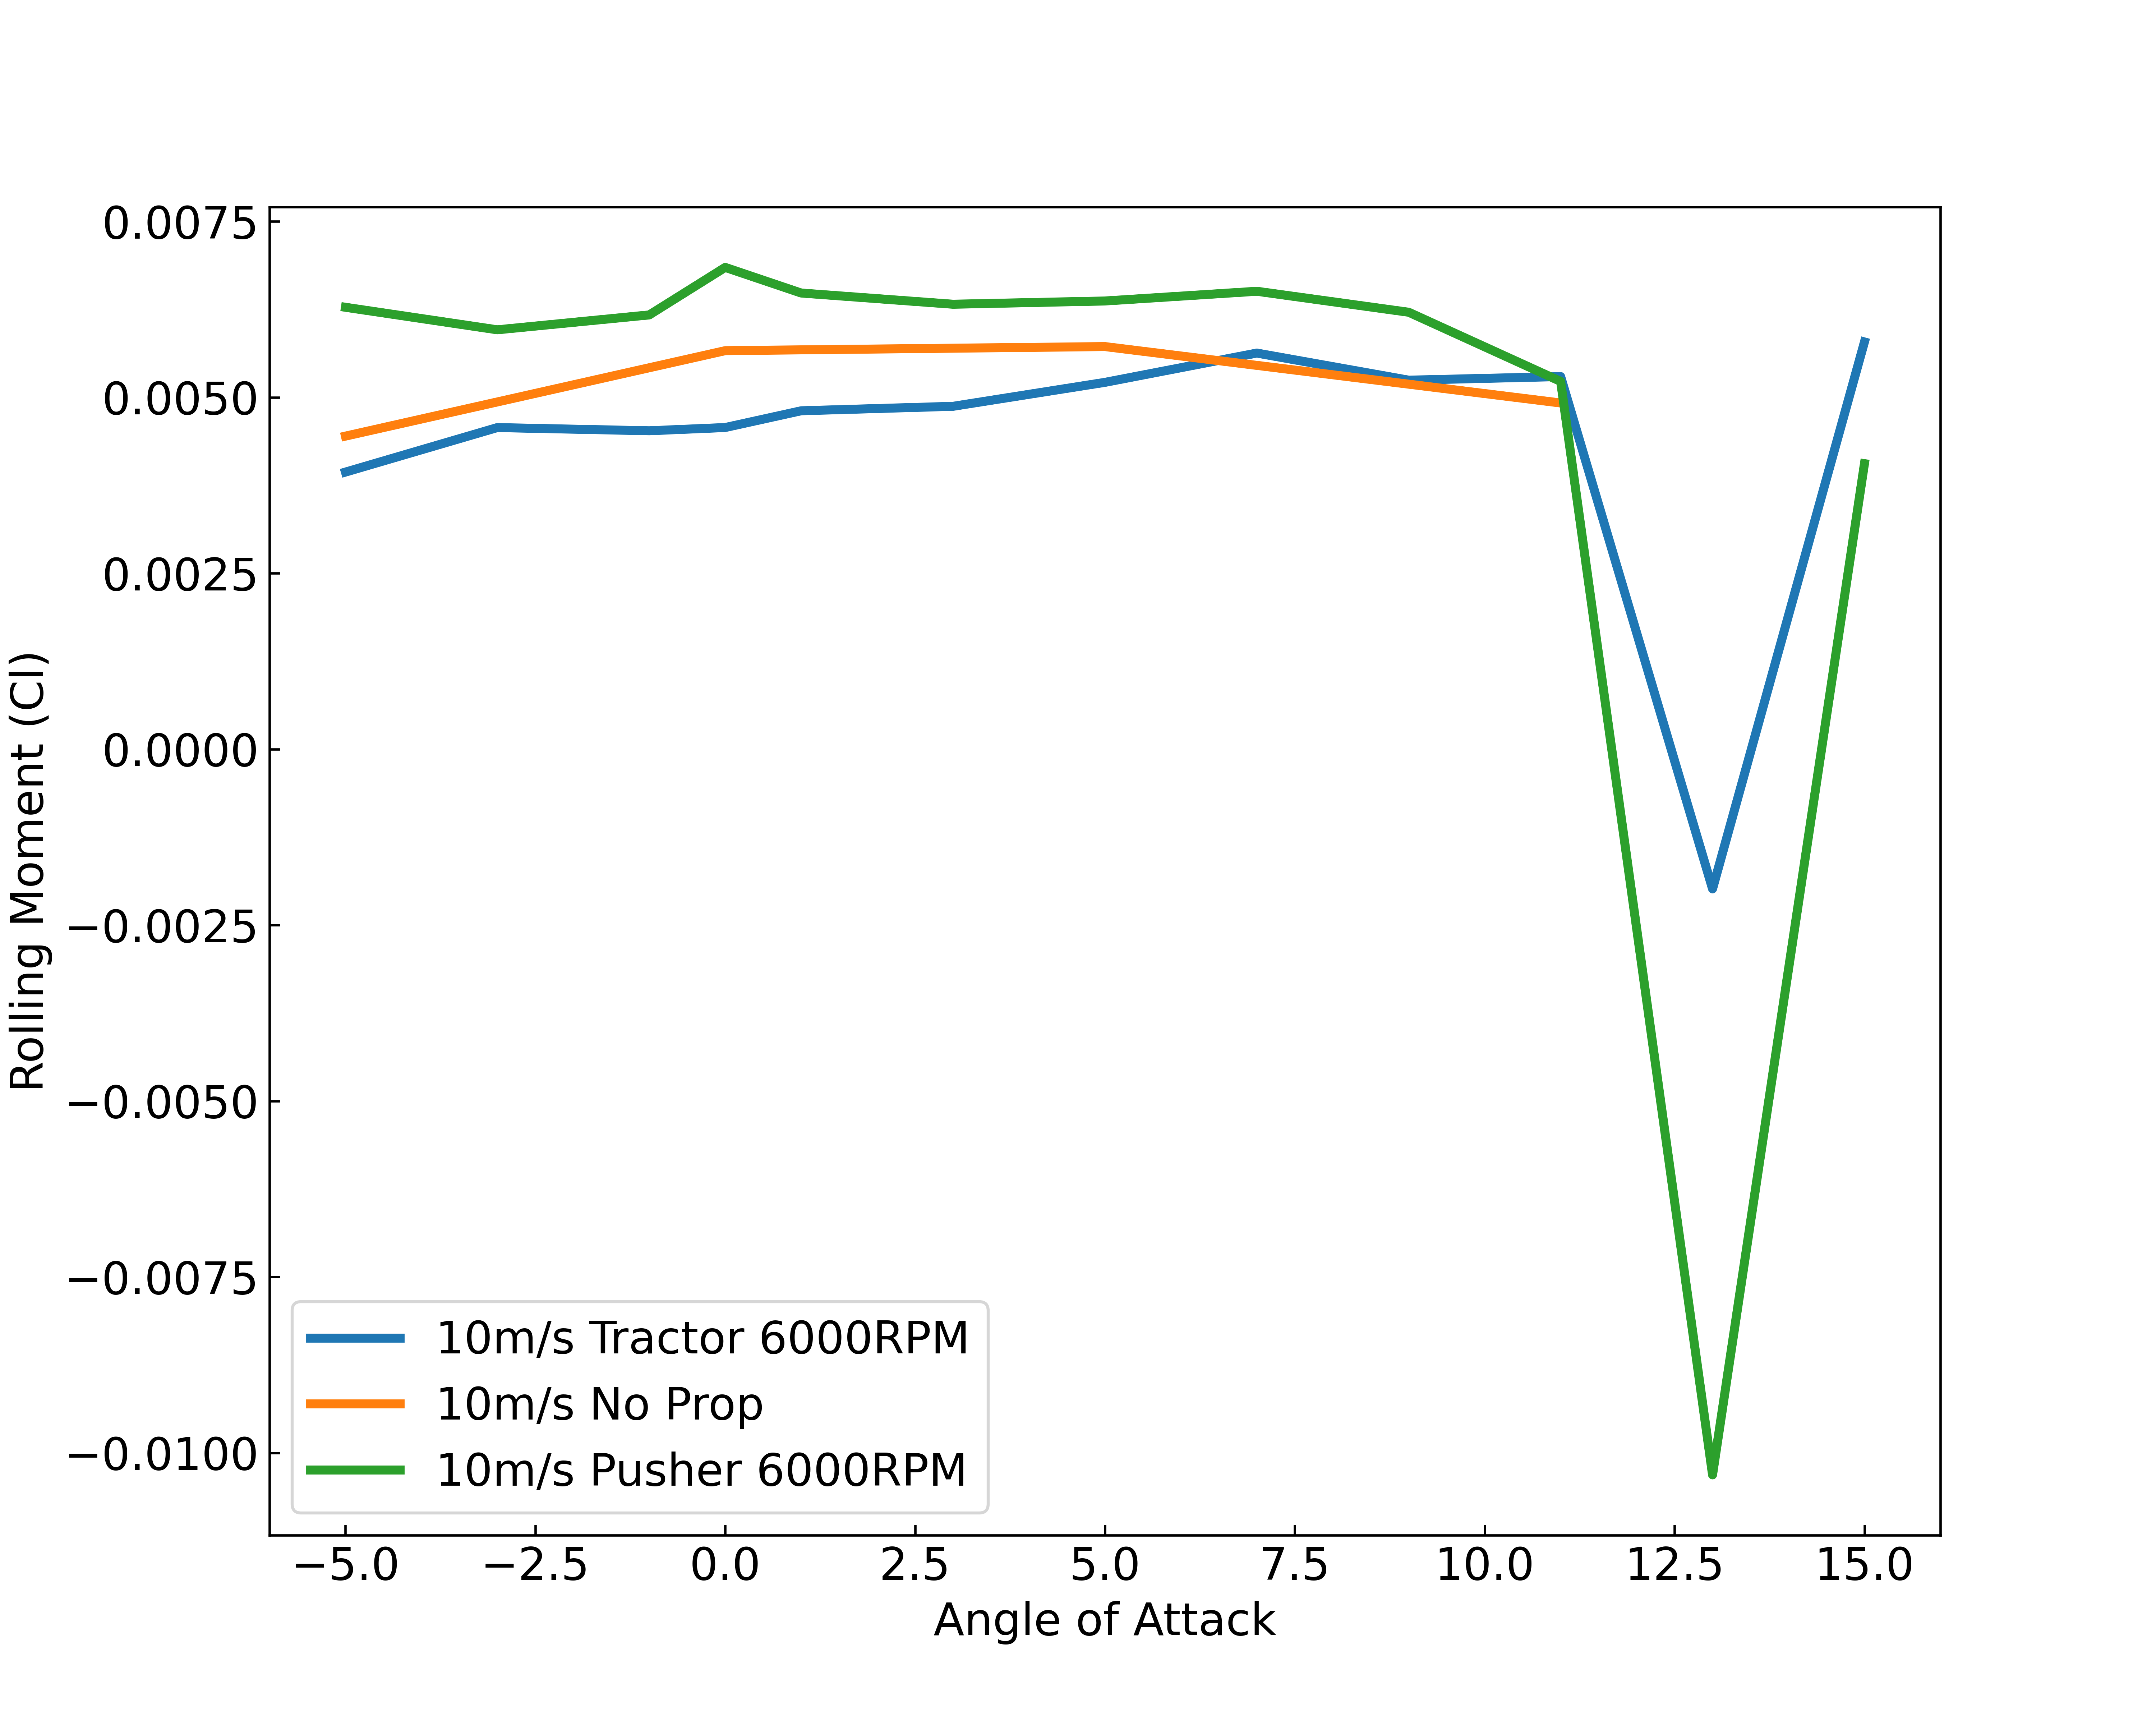
\includegraphics[width=\textwidth]{05_Results/Figs/Cl_roll/10ms_6000RPM_Cl_roll.png}
        \caption{Rolling Moment Coefficient at 10m/s airspeed and 6000RPM motor speed}
        \label{fig:Cl_roll_10ms_6000}
    \end{subfigure}
    \begin{subfigure}[b]{0.467\textwidth}
        \centering
        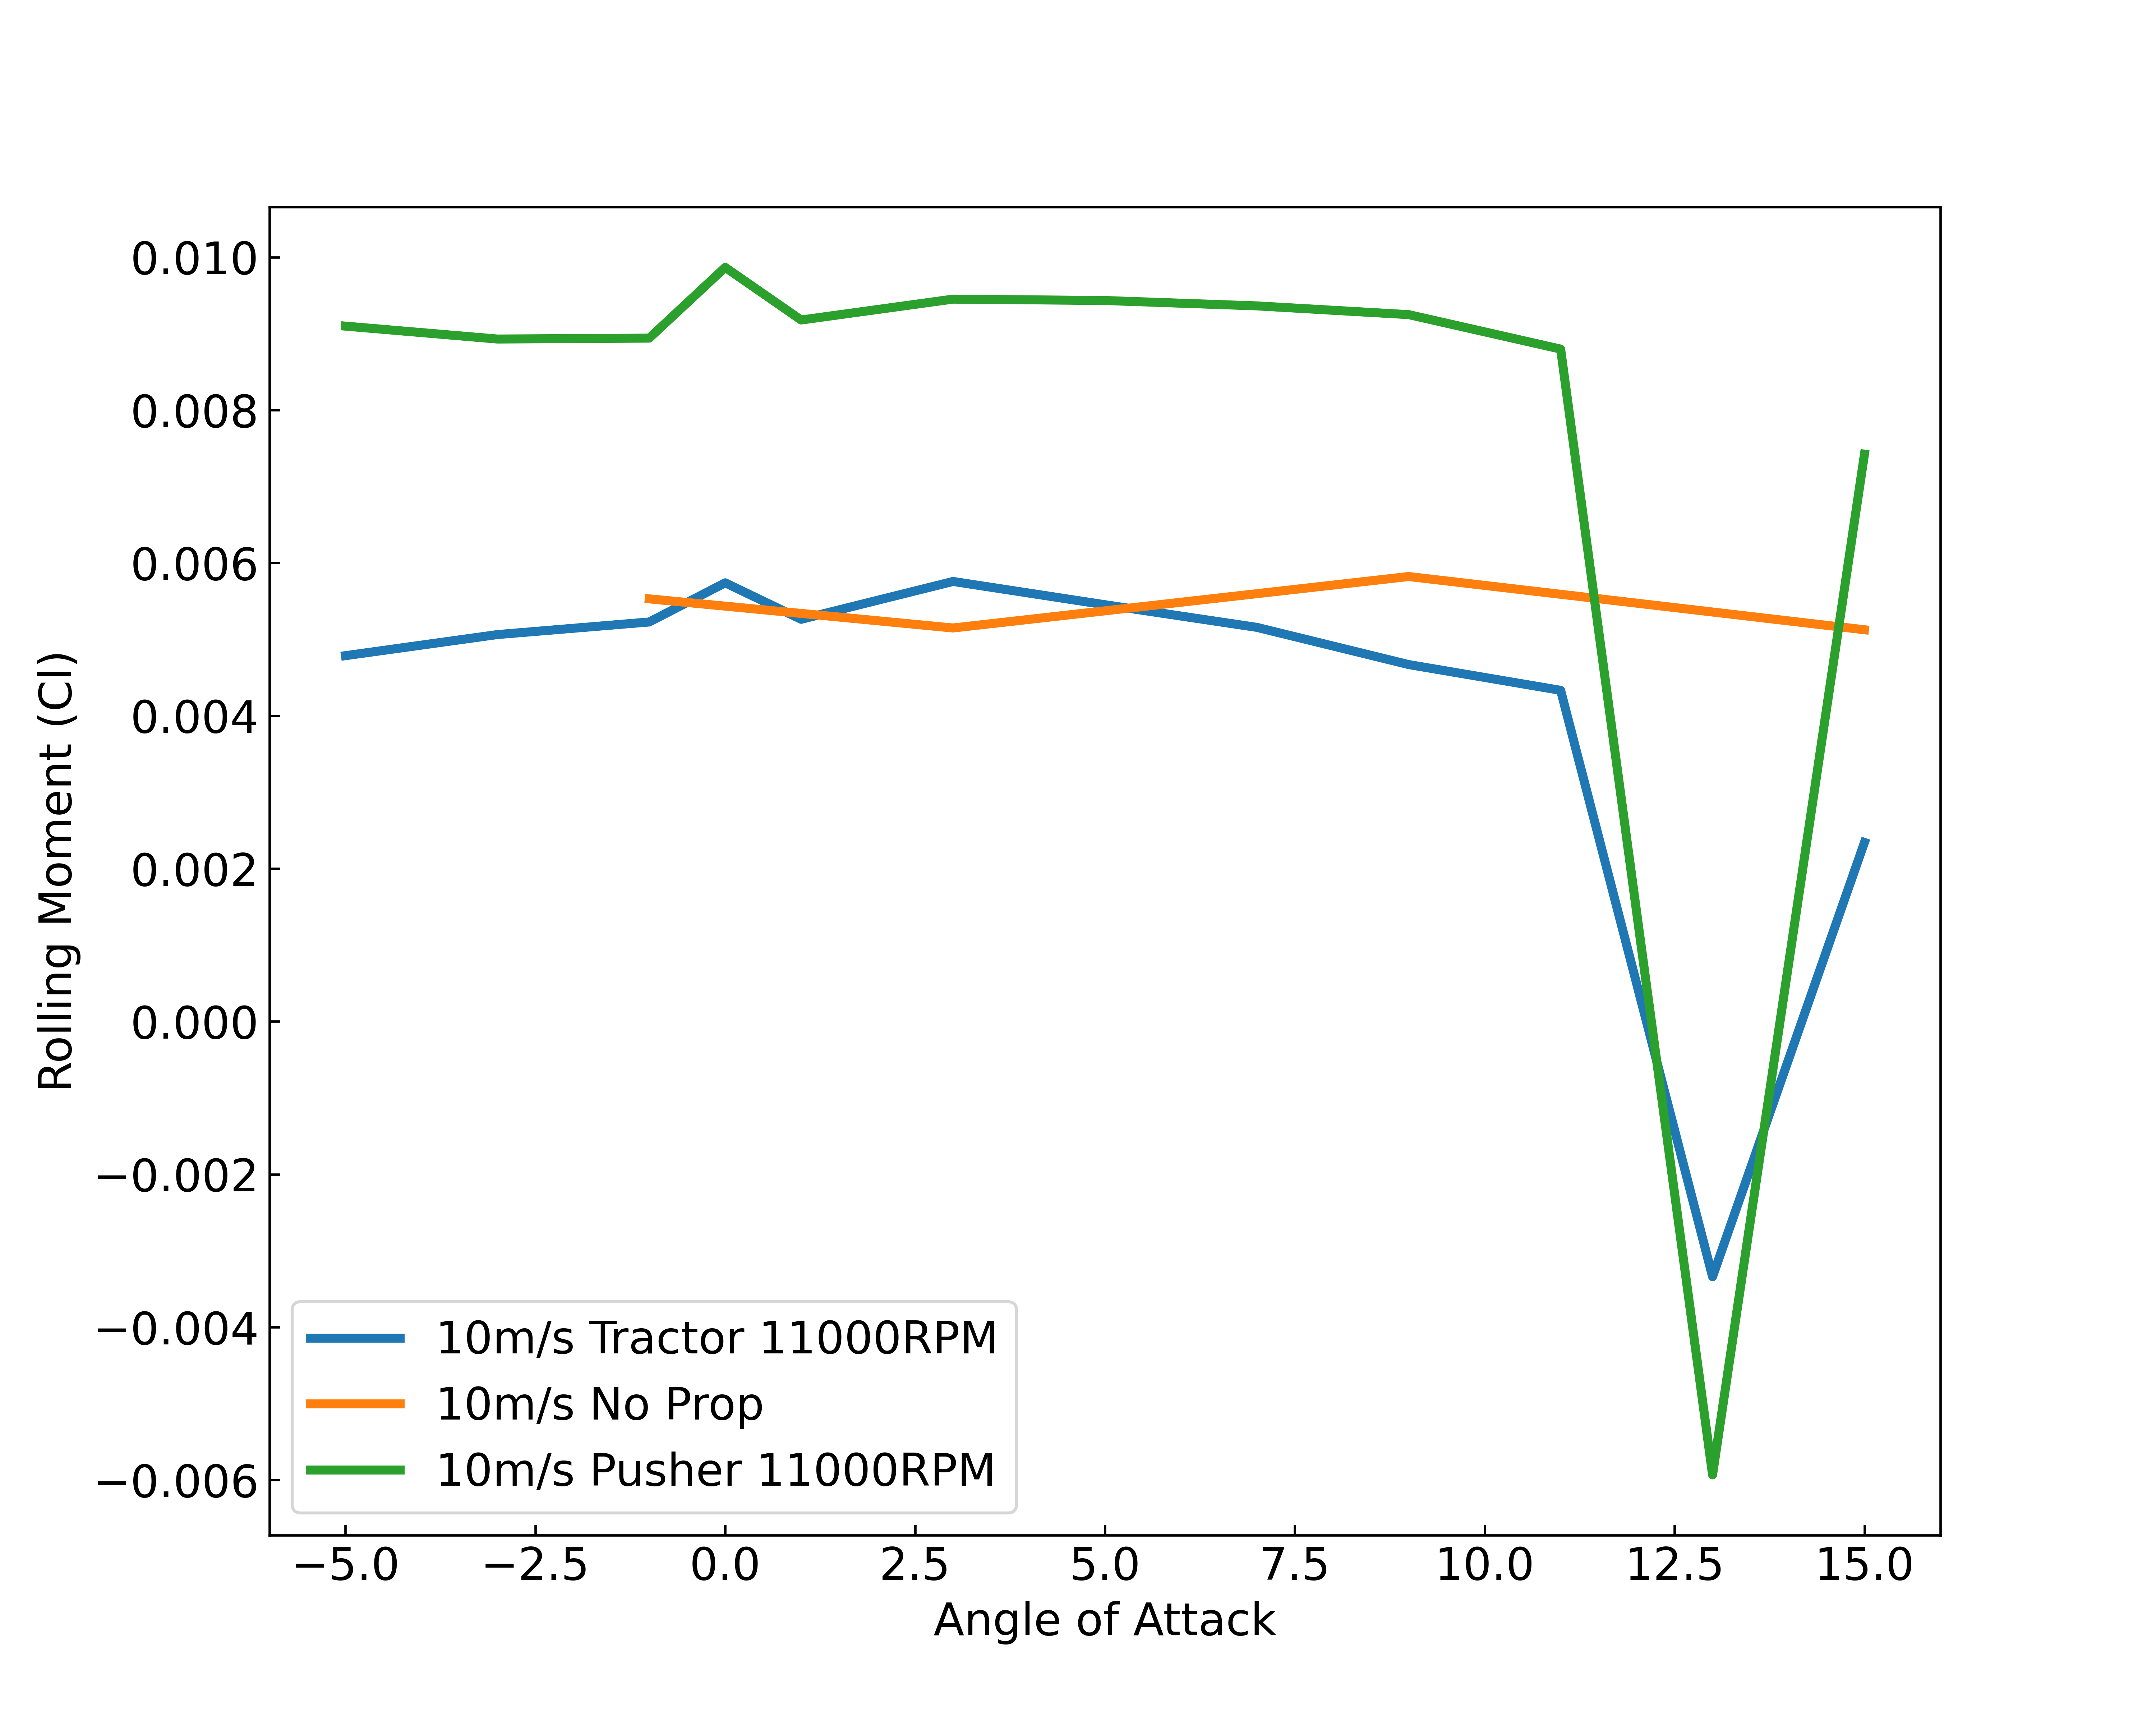
\includegraphics[width=\textwidth]{05_Results/Figs/Cl_roll/10ms_11000RPM_Cl.png}
        \caption{Rolling Moment Coefficient at 10m/s airspeed and 11000RPM motor speed}
        \label{fig:Cl_roll_10ms_11000}
    \end{subfigure}
    \begin{subfigure}[b]{0.467\textwidth}
        \centering
        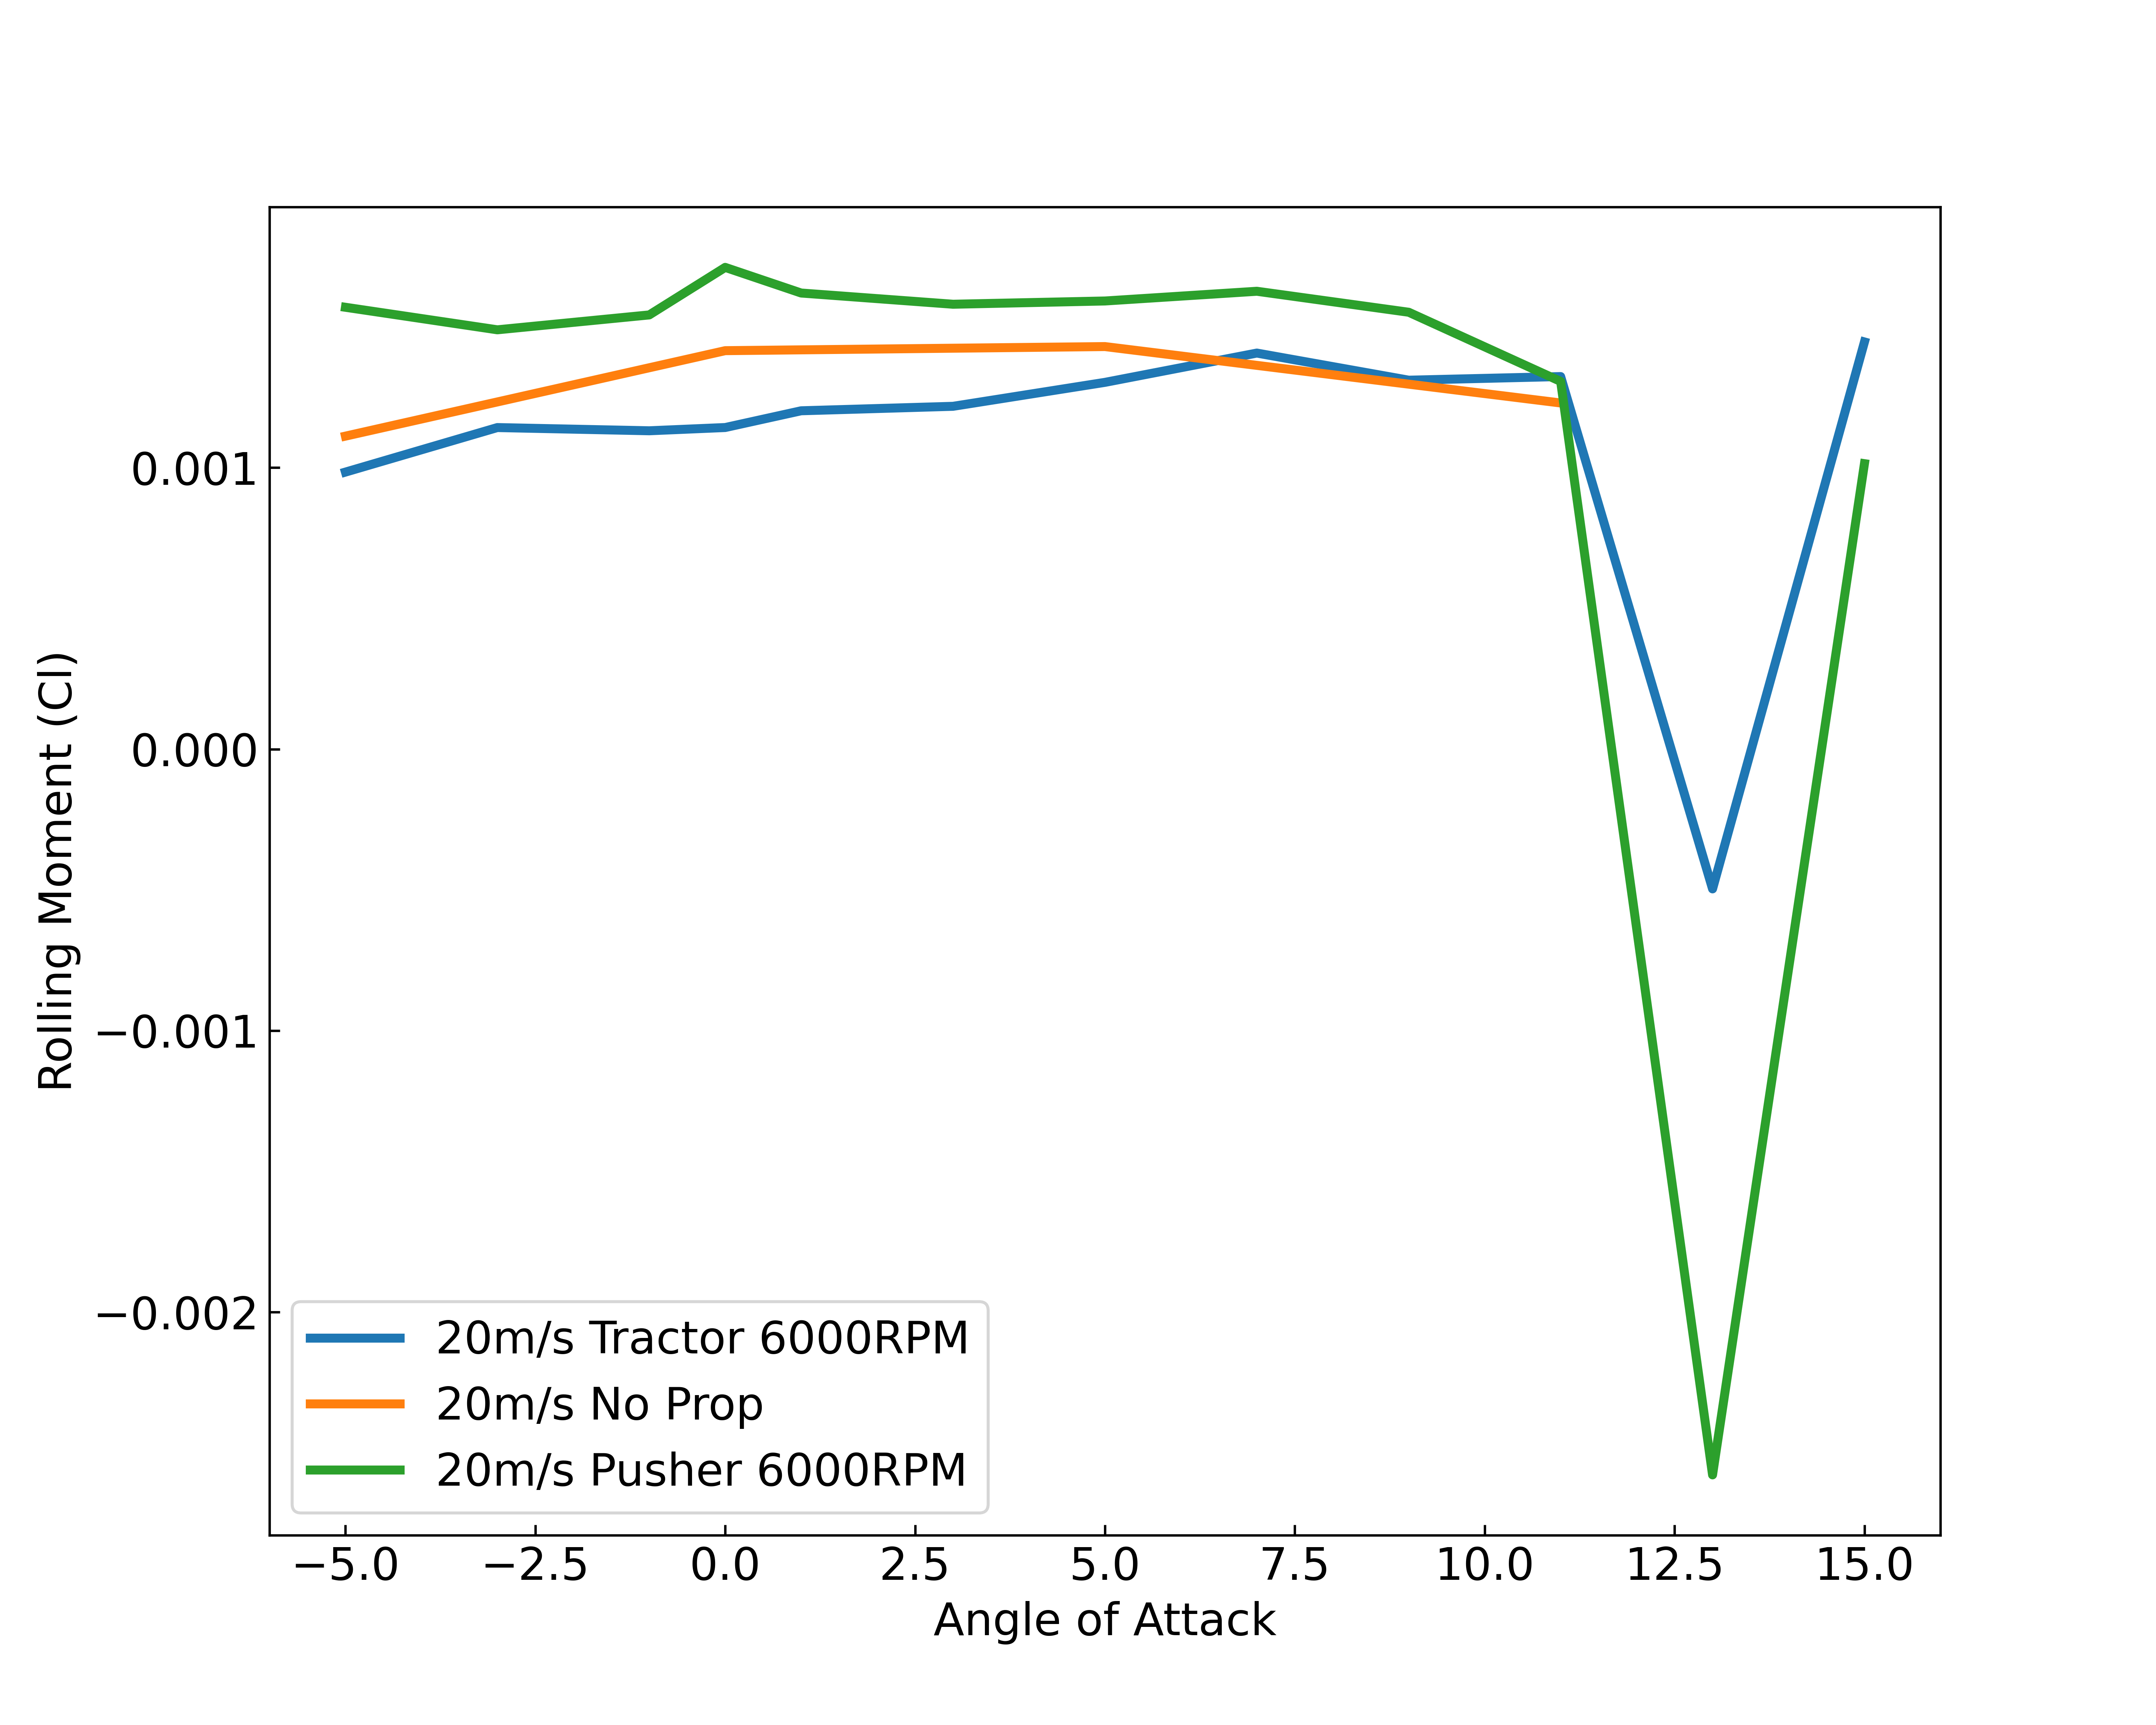
\includegraphics[width=\textwidth]{05_Results/Figs/Cl_roll/20ms_6000RPM_Cl_roll.png}
        \caption{Rolling Moment Coefficient at 20m/s airspeed and 6000RPM motor speed}
        \label{fig:Cl_roll_20ms_6000}
    \end{subfigure}
    \begin{subfigure}[b]{0.467\textwidth}
        \centering
        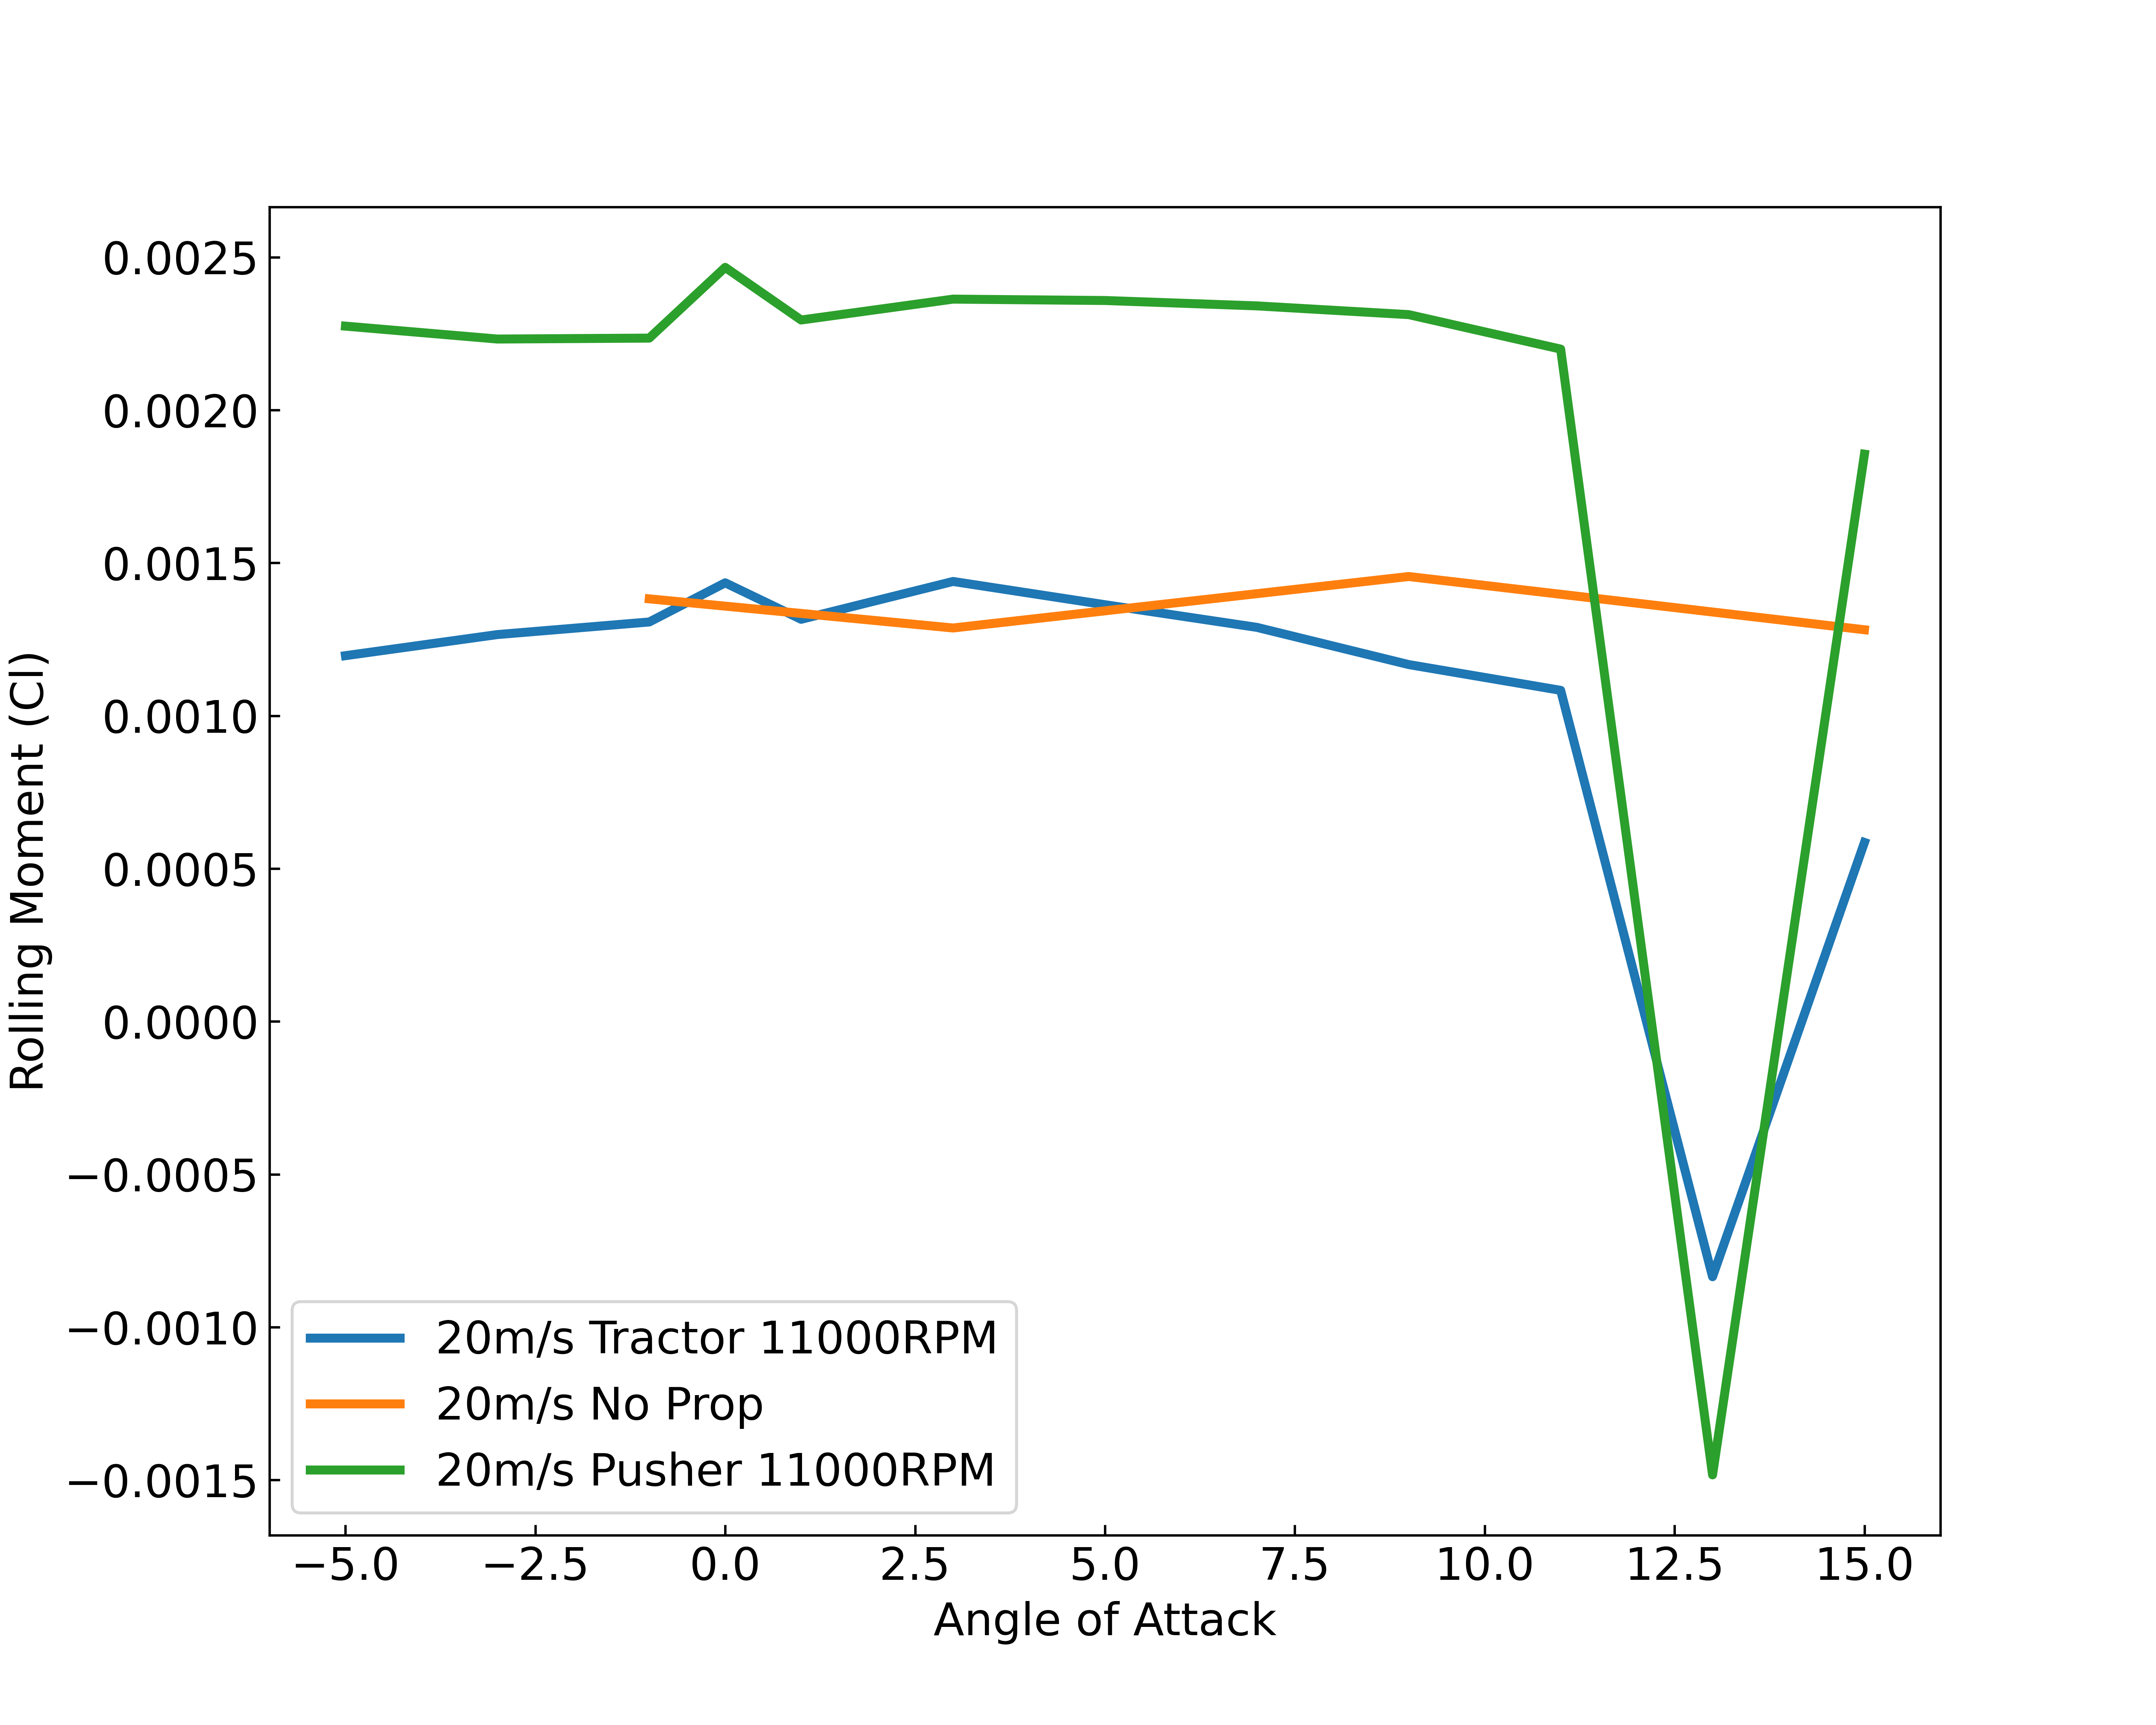
\includegraphics[width=\textwidth]{05_Results/Figs/Cl_roll/20ms_11000RPM_Cl.png}
        \caption{Rolling Moment Coefficient at 20m/s airspeed and 11000RPM motor speed}
        \label{fig:Cl_roll_20ms_11000}
    \end{subfigure}
\end{figure}


\subsection{Yawing Moment Coefficient}
 The yawing coefficient for the tractor configuration was shifted upwards compared to both the pusher and no propeller configurations. The yawing moment is also produced as a consequence of the roll moment produced. The aircraft roll moment remains relatively constant until the stall of the right wing at $\approx$12.5$^{\circ}$ \acrshort{AoA}. Hence the increase in the yawing moment as the aircraft \acrshort{AoA} increases is likely due to the effects of the roll being magnified as flow separation occurs. The roll moment causes an adverse yaw effect where the MAV naturally tends to yaw in the opposite direction of the roll \todo{cite}. This is due to the different lift and drag acting on each wing. As the angle of attack increases, the difference between the two wings in lift and drag increases, leading to an increase in the yaw moment for all configurations, airspeeds and propeller speeds except for the no propeller configuration when run at 20m$s^{-1}$. As the angle of attack increases, the yaw moment increases until sharply dropping off in Figures \Cref{fig:Cl_roll_10ms_6000} to \Cref{fig:Cl_roll_20ms_11000}. This is also due to the stall of the right-wing, creating a lift force imbalance as the left wing continues to produce a lift force while the right-wing experiences flow separation due to the increase in \acrshort{AoA}. The yawing moment also sharply raises as the flow over the left wing also separates and stalls beyond $\approx$12.5$^{\circ}$ \acrshort{AoA}. Several kinks are seen in Figures \Cref{fig:Cl_roll_10ms_6000} to \Cref{fig:Cl_roll_20ms_11000}, the most notable being the changes in gradient seen for the pusher configuration with a propeller speed of 6000RPM in Figures \Cref{fig:Cl_roll_10ms_6000} and \Cref{fig:Cl_roll_20ms_6000} at $\approx$0$^{\circ}$, $\approx$2.5$^{\circ}$ and $\approx$7.5$^{\circ}$\acrshort{AoA}. These changes can be partially attributed to the roll moment changes seen in Figures 
 \Cref{fig:Cl_roll_10ms_6000} to \Cref{fig:Cl_roll_20ms_11000}, which creates an adverse yaw effect that acts opposite to the roll. 

\begin{figure}[H]
    \centering
    \begin{subfigure}[b]{0.467\textwidth}
        \centering
        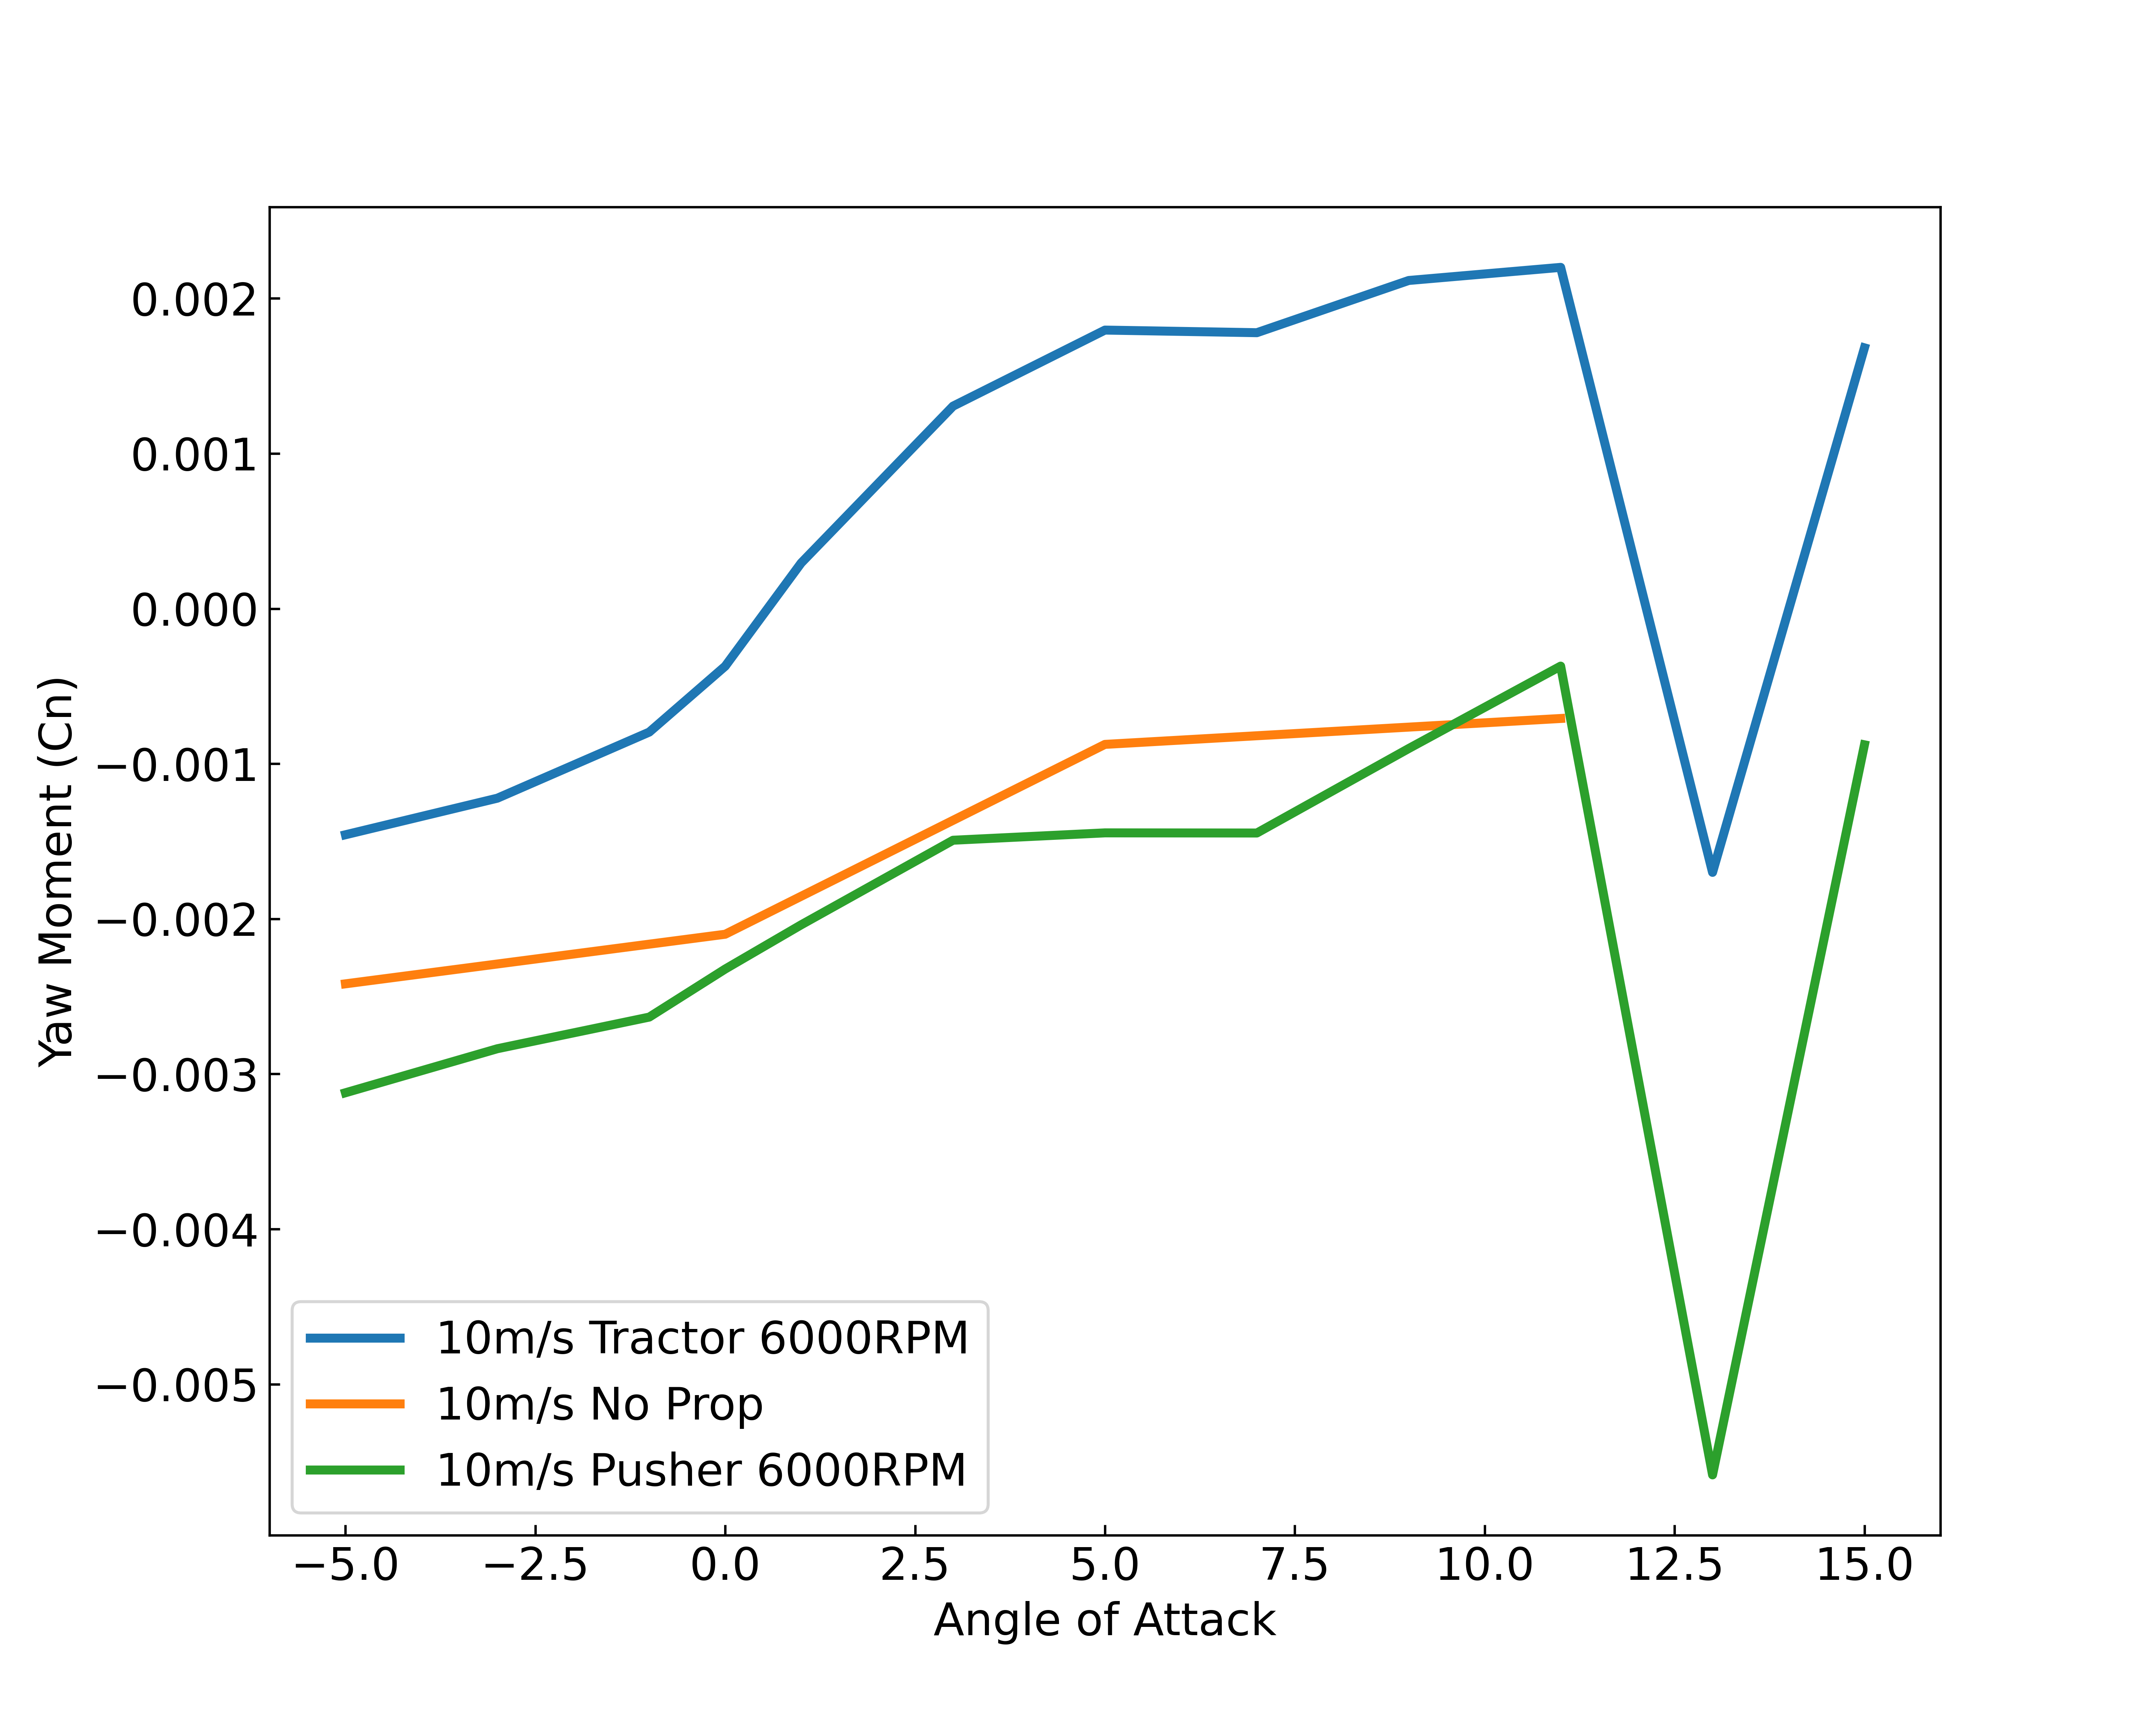
\includegraphics[width=\textwidth]{05_Results/Figs/Cn/10ms_6000RPM_Cn.png}
        \caption{Yawing Moment Coefficient at 10m/s airspeed and 6000RPM motor speed}
        \label{fig:Cn_10ms_6000}
    \end{subfigure}
    \begin{subfigure}[b]{0.467\textwidth}
        \centering
        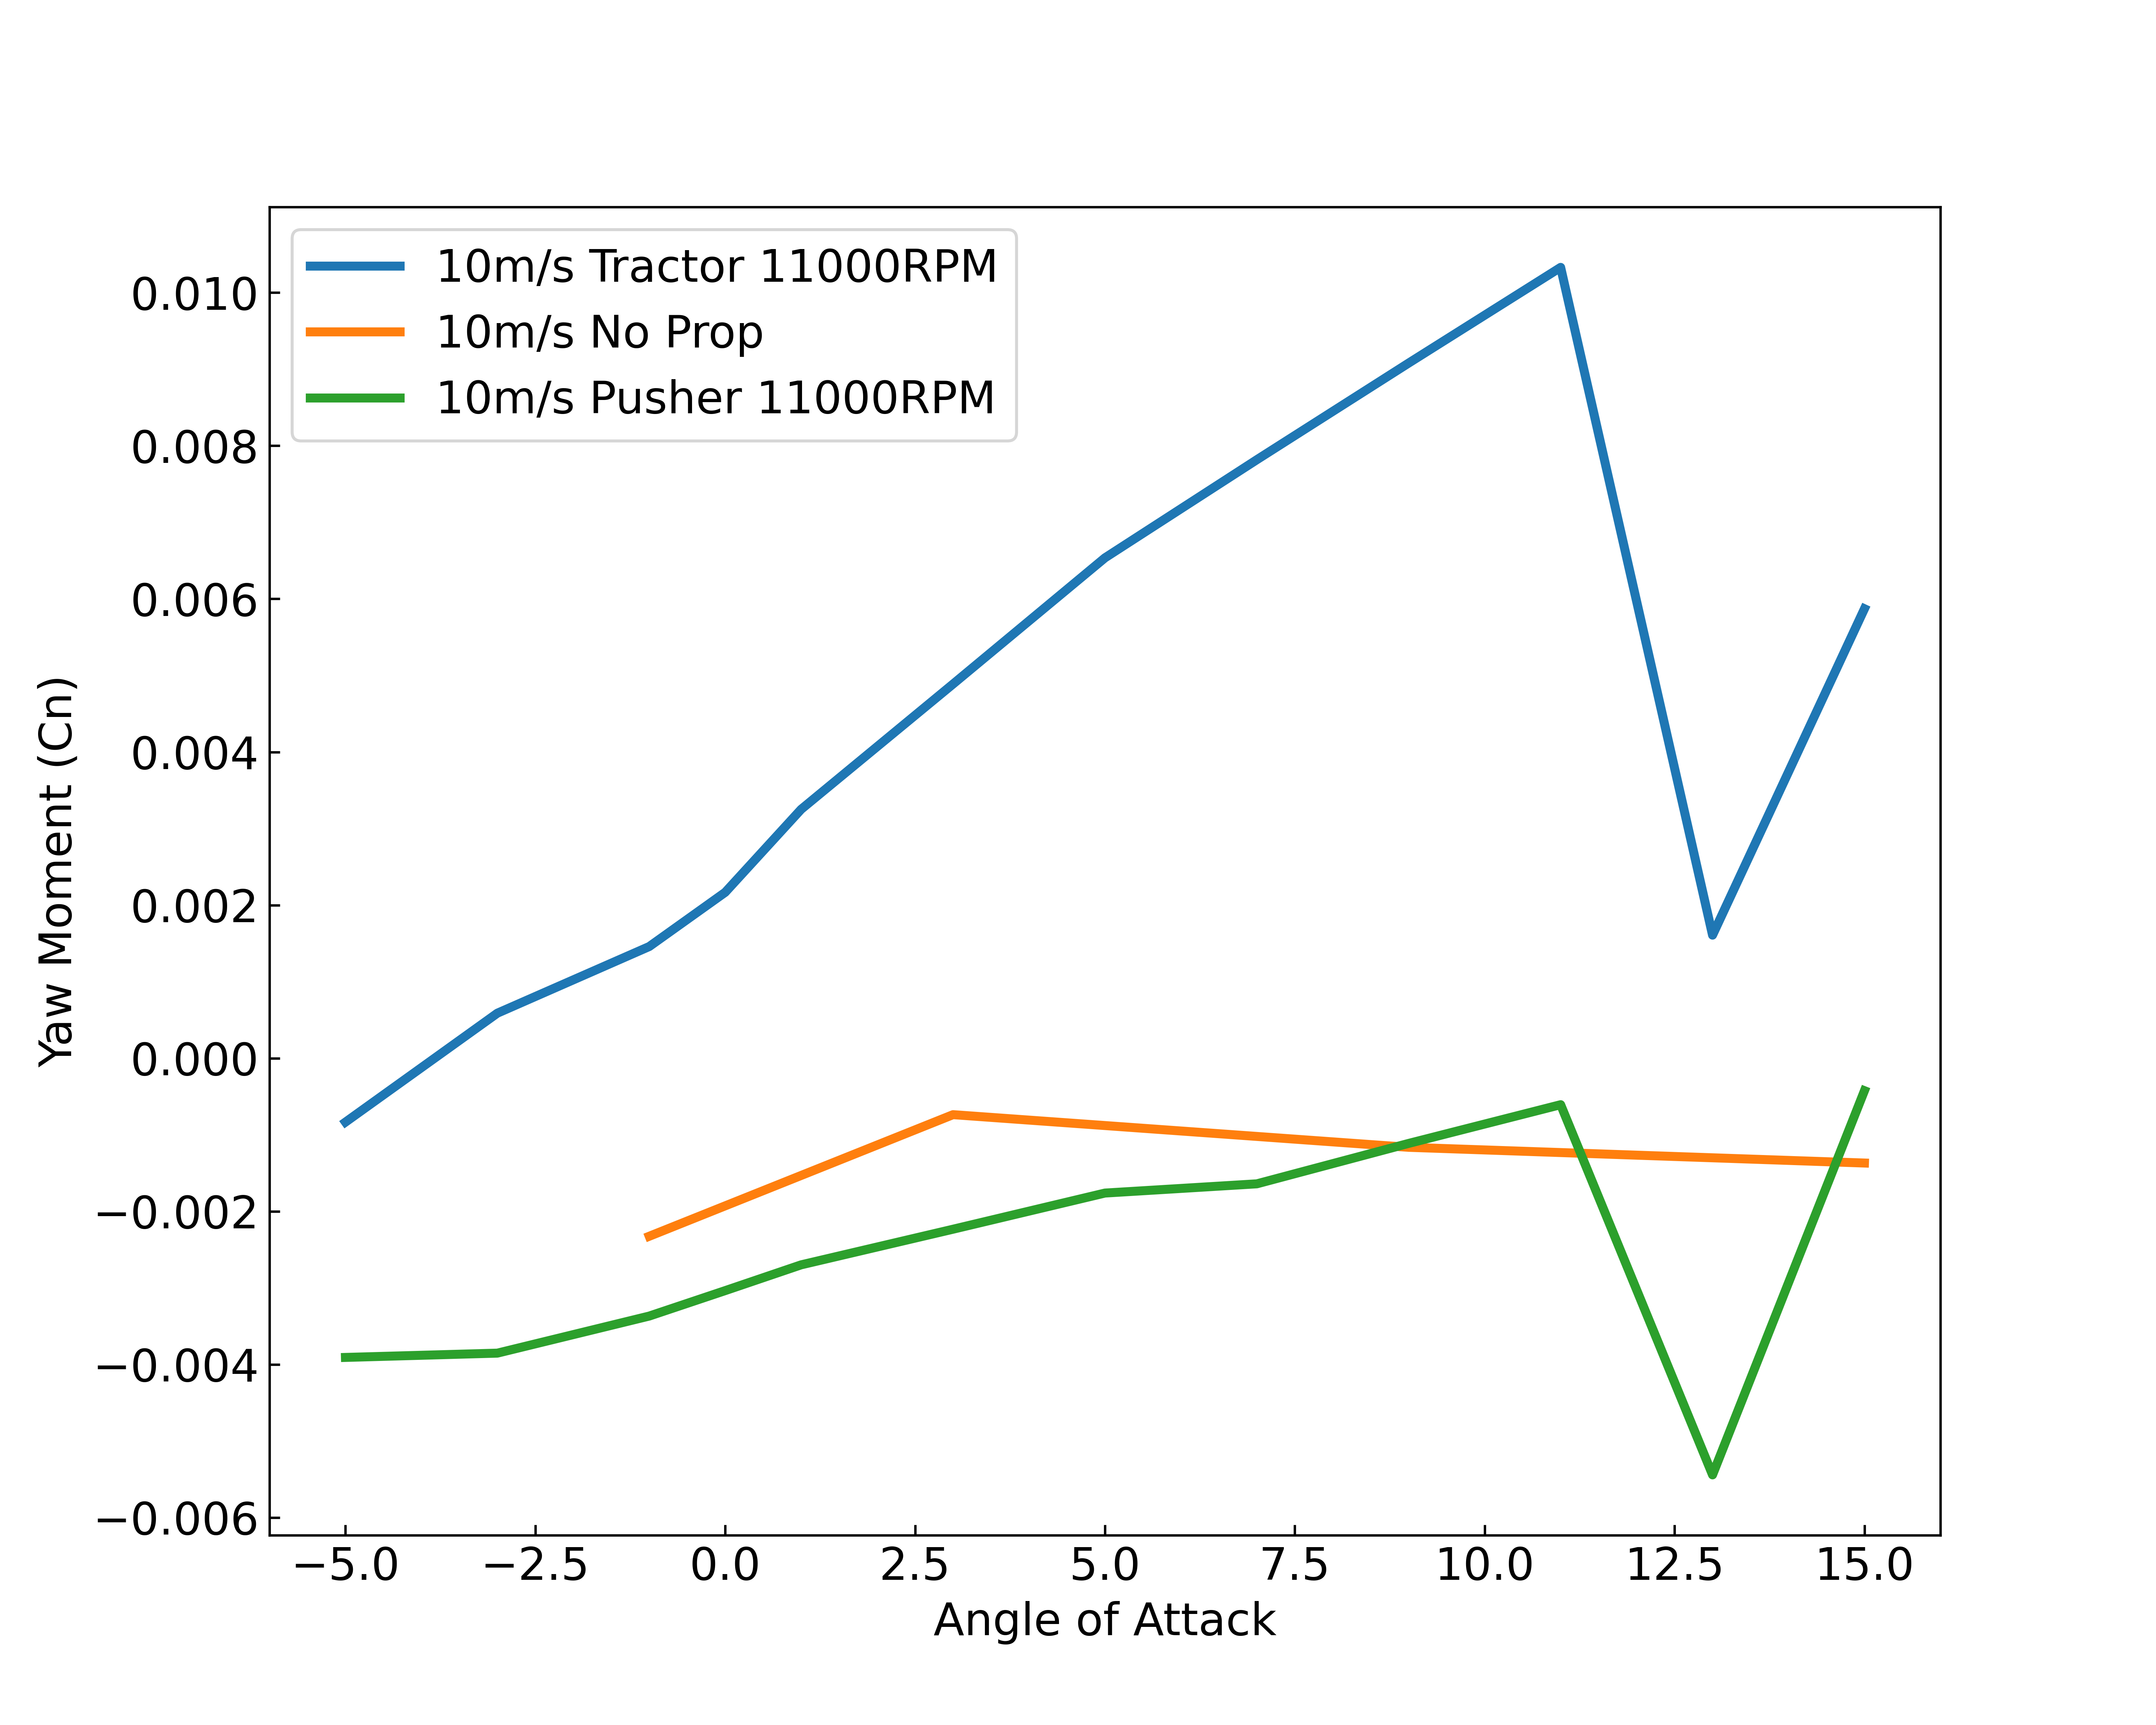
\includegraphics[width=\textwidth]{05_Results/Figs/Cn/10ms_11000RPM_Cn.png}
        \caption{Yawing Moment Coefficient at 10m/s airspeed and 11000RPM motor speed}
        \label{fig:Cn_10ms_11000}
    \end{subfigure}
    \begin{subfigure}[b]{0.467\textwidth}
        \centering
        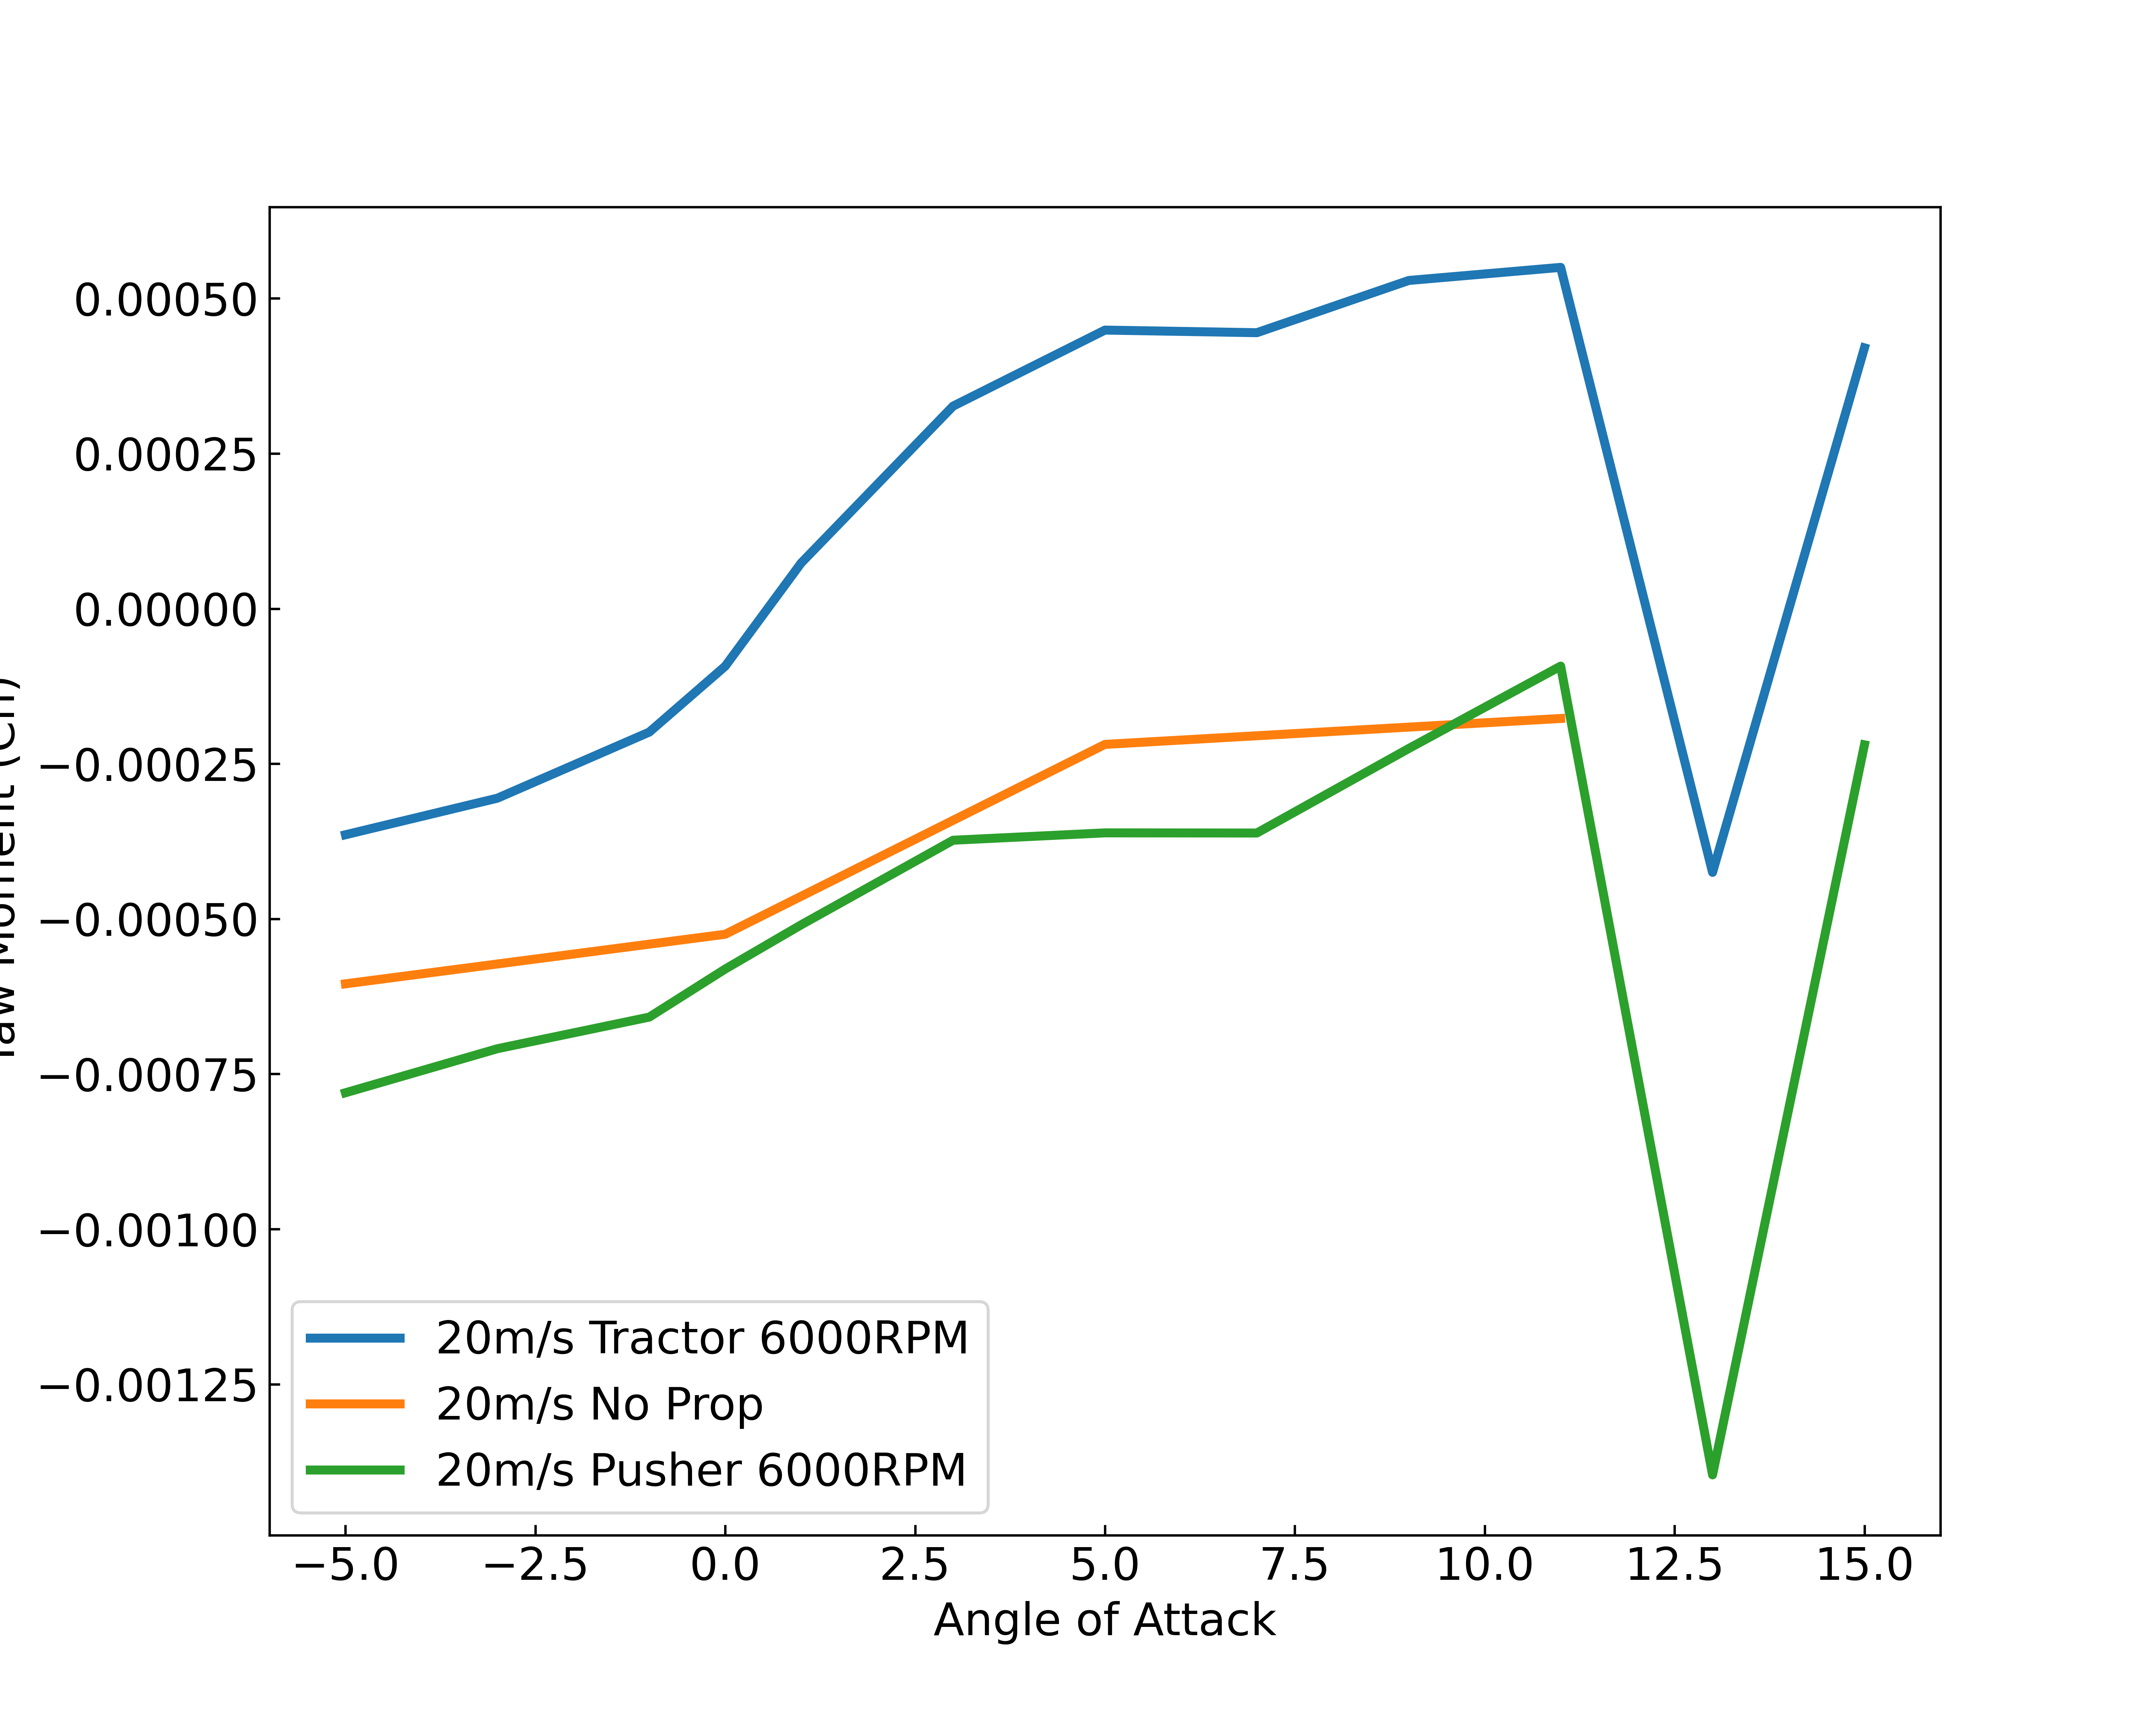
\includegraphics[width=\textwidth]{05_Results/Figs/Cn/20ms_6000RPM_Cn.png}
        \caption{Yawing Moment Coefficient at 20m/s airspeed and 6000RPM motor speed}
        \label{fig:Cn_20ms_6000}
    \end{subfigure}
    \begin{subfigure}[b]{0.467\textwidth}
        \centering
        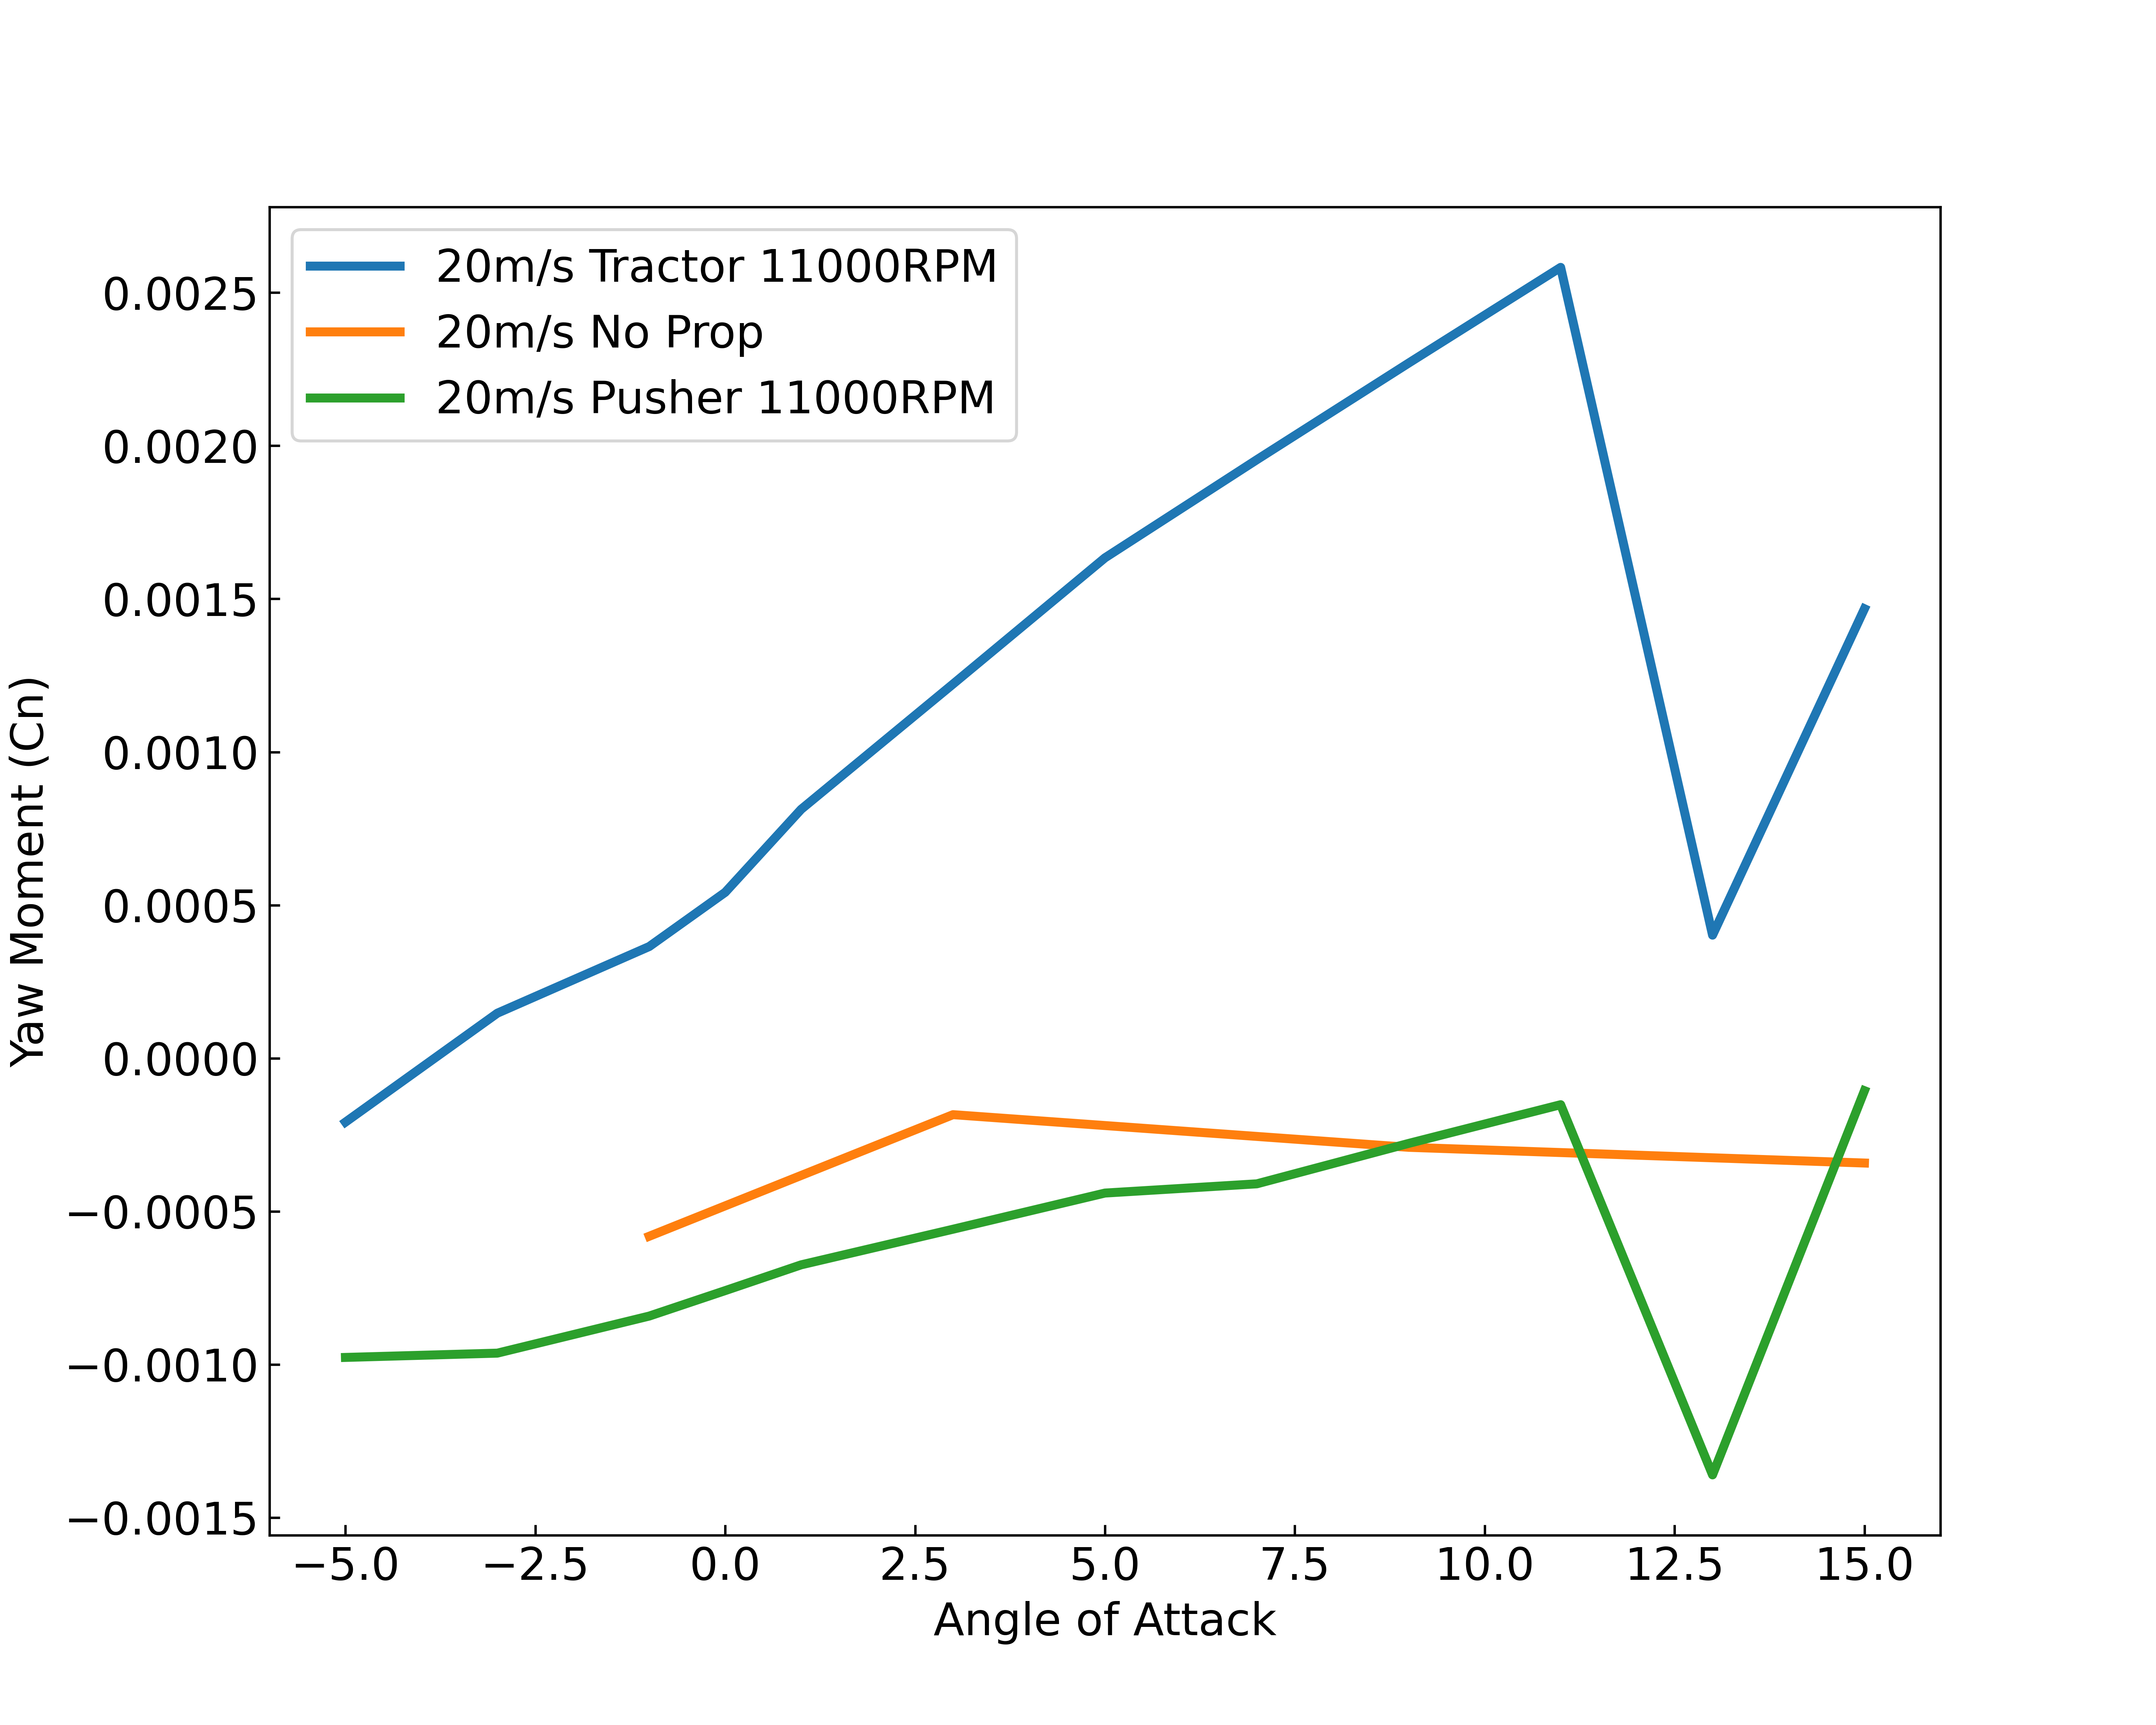
\includegraphics[width=\textwidth]{05_Results/Figs/Cn/20ms_11000RPM_Cn.png}
        \caption{Yawing Moment Coefficient at 20m/s airspeed and 11000RPM motor speed}
        \label{fig:Cn_20ms_11000}
    \end{subfigure}
\end{figure}




\subsection{Static Margin}
The static margin for all configurations shows that  For all airspeeds and propeller speeds tested the tractor configuration decreased the stability of the MAV with the exception of the 10m$s^{-1}$ at 6000RPM propeller speed. This is also seen more clearly in Table \ref{tab:staticMargin} as static margin decreases from -0.155 to -0.107 when comparing the no propeller and tractor configurations at 11000RPM and  10m$s^{-1}$. At 6000RPM propeller speed the tractor configuration became less stable when airspeed increased from 10m$s^{-1}$ to 20m$s^{-1}$, with the static margin decreasing from -0.116 to -0.106. This same trend was also seen for the pusher configuration at 6000RPM propeller speed, decreasing from -0.117 to -0.108. The opposite trend was seen when the propeller speed was increased to 11000RPM. The tractor and pusher configurations became more stable, increasing from -0.107 to -0.118 and from -0.156 to -0.173 respectively when  airspeed increased from 10m$s^{-1}$ to 20m$s^{-1}$. The no propeller configuration became more stable at all propeller speeds as the airspeed increased from 10m$s^{-1}$ to 20m$s^{-1}$.


\begin{tabular}{ |c|c|c|c| }
 \hline

 \hline
 Configuration & Airspeed (ms$^{-1}$ &  Propeller Speed (RPM) & Static Margin\\
 \hline
 Tractor & 10 & 6000 & -0.116 \\
 Tractor & 20 & 6000 & -0.106\\
No Propeller & 10 & 6000 & -0.100\\
  No Propeller & 20 & 6000 & -0.107 \\
 Pusher & 10 & 6000 & -0.117 \\
  Pusher & 20 & 6000 & -0.108 \\
  \hline
 Tractor & 10 & 11000 & -0.107 \\
 Tractor & 20 & 11000 & -0.118\\
 No Propeller & 10 & 11000 & -0.155\\
 No Propeller& 20 & 11000 & -0.159\\
 Pusher & 10 & 11000 & -0.156 \\
 Pusher & 20 & 11000 & -0.173 \\
 \hline
 \label{tab:staticMargin}
\end{tabular}



\begin{figure}[H]
    \centering
    \begin{subfigure}[b]{0.467\textwidth}
        \centering
        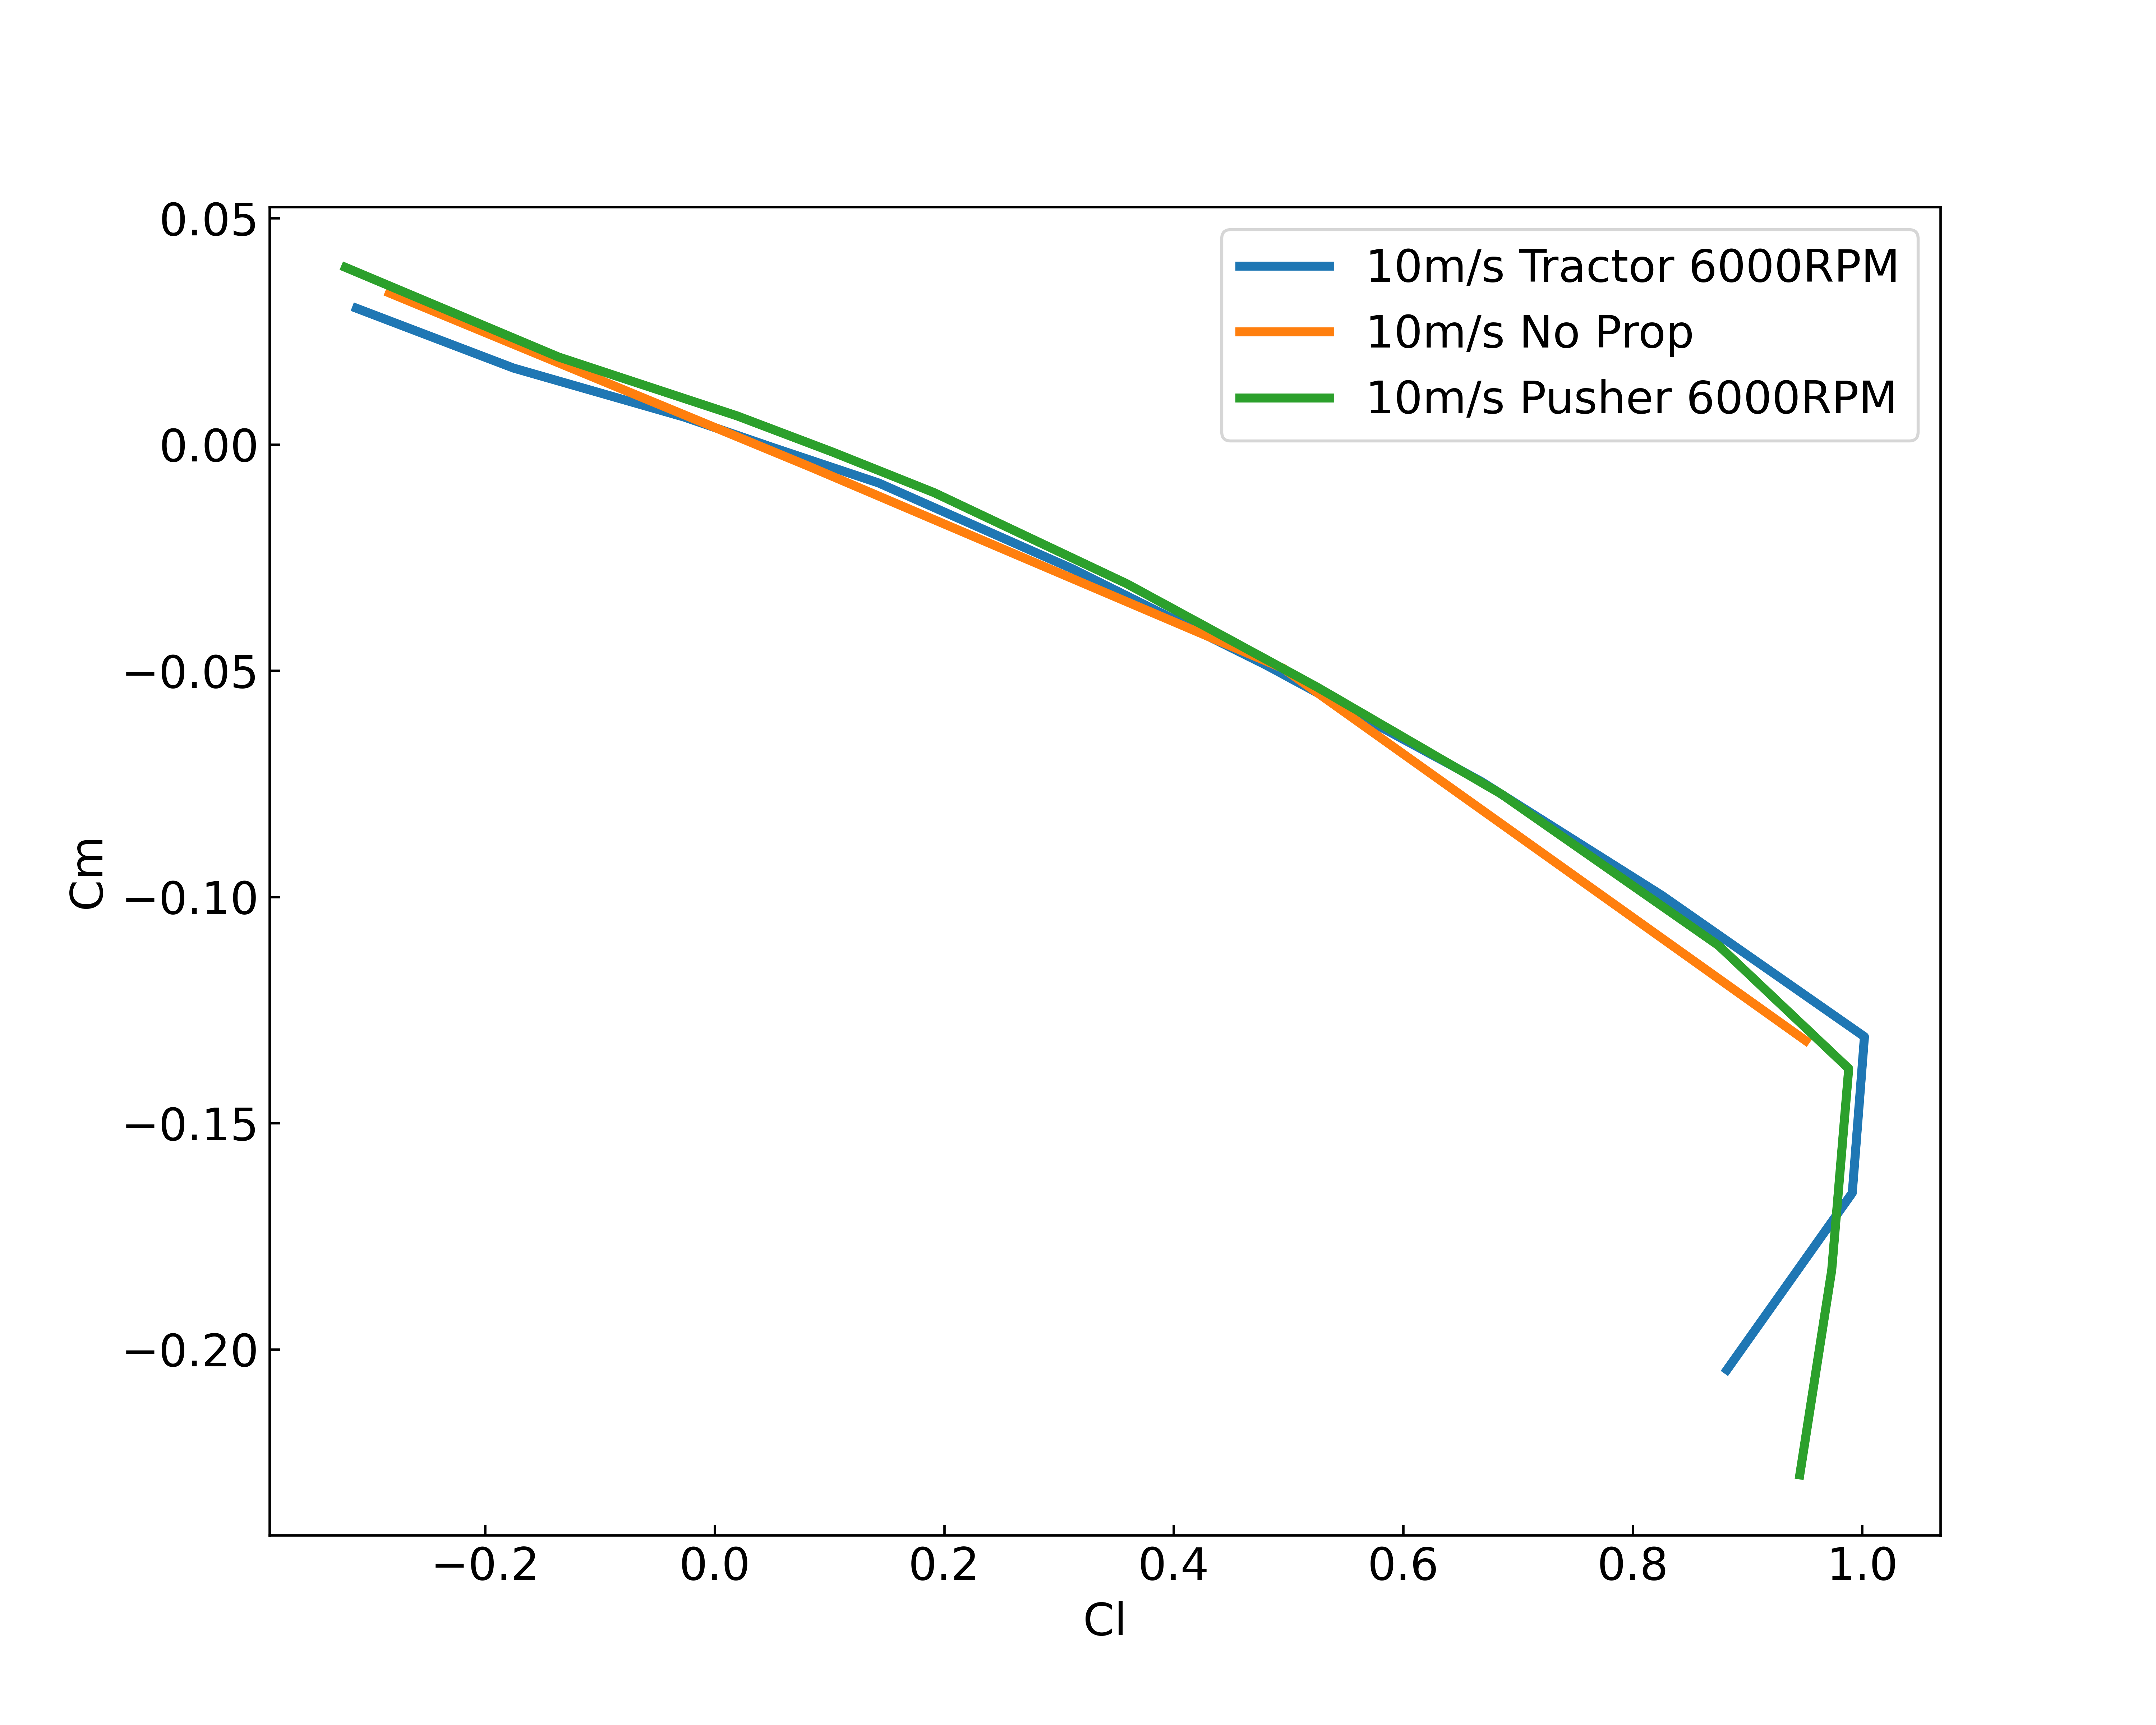
\includegraphics[width=\textwidth]{05_Results/Figs/ClCm/10ms_6000RPM_CmCl.png}
        \caption{Rolling Moment Coefficient at 10m/s airspeed and 6000RPM motor speed}
        \label{fig:CmCl_10ms_6000}
    \end{subfigure}
    \begin{subfigure}[b]{0.467\textwidth}
        \centering
        \includegraphics[width=\textwidth]{05_Results/Figs/ClCm/10ms_11000RPM_CmCl.png}
        \caption{Rolling Moment Coefficient at 10m/s airspeed and 11000RPM motor speed}
        \label{fig:CmCl_10ms_11000}
    \end{subfigure}
    \begin{subfigure}[b]{0.467\textwidth}
        \centering
        \includegraphics[width=\textwidth]{05_Results/Figs/ClCm/20ms_6000RPM_CmCl.png}
        \caption{Rolling Moment Coefficient at 20m/s airspeed and 6000RPM motor speed}
        \label{fig:CmCl_20ms_6000}
    \end{subfigure}
    \begin{subfigure}[b]{0.467\textwidth}
        \centering
        \includegraphics[width=\textwidth]{05_Results/Figs/ClCm/20ms_11000RPM_CmCl.png}
        \caption{Rolling Moment Coefficient at 20m/s airspeed and 11000RPM motor speed}
        \label{fig:CmCl_20ms_11000}
    \end{subfigure}
\end{figure}


\section{VAP 3.5 Validation}
Low speed aerodynamics generally see complex flow distributions and phenomena as dicussed in Sections \ref{sec:Reynolds} and \ref{sec:Reynolds2}. In order to evaluate the usage of VAP 3.5 for the wind tunnel tests conducted, a wing validation and model validation was performed with comparison to the GenMAV model which has been previously evaluated with the Athena Vortex Lattice (AVL) method in order to estimate the stability derivatives and moments of the GenMAV. 

\subsection{Wing Validation}
A wing validation against Fluent CFD results is given in Figures \ref{fig:wing0300} to Figure \ref{fig:001000b} \cite{}. This data was taken at a Reynolds number of 2.32 $\times 10^{5}$ at a freestream velocity of 20$m/s$ and density 1.225$kg/m^3$. 

\begin{figure}[H]
     \centering
     \begin{subfigure}[b]{0.45\textwidth}
         \centering
         \includegraphics[width=\textwidth]{05_Results/Figs/VAP/genMAV/taper3a.png}
         \caption{}
         \label{fig:wing0300}

     \end{subfigure}
     \hfill
     \begin{subfigure}[b]{0.45\textwidth}
         \centering
         \includegraphics[width=\textwidth]{05_Results/Figs/VAP/genMAV/taper3b.png}
         \caption{}
         \label{fig:wing0300b}
      
     \end{subfigure}
     \hfill

        
\end{figure}


\begin{figure}[H]
     \centering
     \begin{subfigure}[b]{0.45\textwidth}
         \centering
         \includegraphics[width=\textwidth]{05_Results/Figs/VAP/genMAV/taper5a.png}

     \end{subfigure}
     \hfill
     \begin{subfigure}[b]{0.45\textwidth}
         \centering
         \includegraphics[width=\textwidth]{05_Results/Figs/VAP/genMAV/taper5b.png}
      
     \end{subfigure}
     \hfill

        
\end{figure}


\begin{figure}[H]
     \centering
     \begin{subfigure}[b]{0.45\textwidth}
         \centering
         \includegraphics[width=\textwidth]{05_Results/Figs/VAP/genMAV/taper10a.png}

     \end{subfigure}
     \hfill
     \begin{subfigure}[b]{0.45\textwidth}
         \centering
         \includegraphics[width=\textwidth]{05_Results/Figs/VAP/genMAV/taper10b.png}
         \caption{}
         
      \label{fig:001000b}
     \end{subfigure}
     \hfill

        
\end{figure}


\subsection{GenMAV model validation}


\begin{figure}[H]
     \centering
     \begin{subfigure}[b]{0.45\textwidth}
          \centering
        \includegraphics[width=\textwidth]{05_Results/Figs/VAP/genMAV/dimensions.png}
            \label{fig:genMAVDimensions}

     \end{subfigure}
     \hfill
     \begin{subfigure}[b]{0.45\textwidth}
                \centering
            \includegraphics[width=\textwidth]{05_Results/Figs/VAP/genMAV/GenMAVModelValidation1.png}
             \label{fig:genMAV_Cm}
              \caption{}
     \end{subfigure}
     \hfill

        
\end{figure}


\begin{figure}[H]
     \centering
     \begin{subfigure}[b]{0.45\textwidth}
            \centering
         \includegraphics[width=\textwidth]{05_Results/Figs/VAP/genMAV/GenMAVModelValidation2.png}
         \label{fig:genMAV_Cl_roll}
         \caption{}

     \end{subfigure}
     \hfill
     \begin{subfigure}[b]{0.45\textwidth}
               \centering
         \includegraphics[width=\textwidth]{05_Results/Figs/VAP/genMAV/GenMAVModelValidation3.png}
         \label{fig:genMAV_Cn}
         \caption{}
     \end{subfigure}
     \hfill
\end{figure}



\begin{figure}[H]
    \centering
    \includegraphics[width=0.5\textwidth]{05_Results/Figs/VAP/genMAV/dimensions.png}
    \label{fig:genMAVDimensions}
\end{figure}

\begin{figure}[H]
         \centering
         \includegraphics[width=0.5\textwidth]{05_Results/Figs/VAP/genMAV/GenMAVModelValidation1.png}
         \label{fig:genMAV_Cm}
         \caption{}
\end{figure}

% \begin{figure}[H]
       
% \end{figure}

% \begin{figure}
       
% \end{figure}

\subsection{Validation of Wind Tunnel Results with VAP 3.5}
side forces and moments still in testing for VAP 3.5

\subsubsection{No Propeller Configuration}


\begin{figure}[H]
    \centering
    \begin{subfigure}[b]{0.467\textwidth}
        \centering
        \includegraphics[width=\textwidth]{05_Results/VAP/noProp/Cl/10ms_6000RPM_Cl.png}
        \caption{Rolling Moment Coefficient at 10m/s airspeed and 6000RPM motor speed}
        \label{fig:VAP_NoProp_Cl_10ms_6000}
    \end{subfigure}
    \begin{subfigure}[b]{0.467\textwidth}
        \centering
        \includegraphics[width=\textwidth]{05_Results/VAP/noProp/Cl/10ms_11000RPM_Cl.png}
        \caption{Rolling Moment Coefficient at 10m/s airspeed and 11000RPM motor speed}
        \label{fig:VAP_NoProp_Cl_10ms_11000}
    \end{subfigure}
    \begin{subfigure}[b]{0.467\textwidth}
        \centering
        \includegraphics[width=\textwidth]{05_Results/VAP/noProp/Cl/20ms_6000RPM_Cl.png}
        \caption{Rolling Moment Coefficient at 20m/s airspeed and 6000RPM motor speed}
        \label{fig:VAP_NoProp_Cl_20ms_6000}
    \end{subfigure}
    \begin{subfigure}[b]{0.467\textwidth}
        \centering
        \includegraphics[width=\textwidth]{05_Results/VAP/noProp/Cl/20ms_11000RPM_Cl.png}
        \caption{Rolling Moment Coefficient at 20m/s airspeed and 11000RPM motor speed}
        \label{fig:VAP_NoProp_Cl_20ms_11000}
    \end{subfigure}
\end{figure}


\begin{figure}[H]
    \centering
    \begin{subfigure}[b]{0.467\textwidth}
        \centering
        \includegraphics[width=\textwidth]{05_Results/VAP/noProp/Cm/10ms_6000RPM_Cm.png}
        \caption{Pitching Moment Coefficient at 10m/s airspeed and 6000RPM motor speed}
        \label{fig:VAP_NoProp_Cm_10ms_6000}
    \end{subfigure}
    \begin{subfigure}[b]{0.467\textwidth}
        \centering
        \includegraphics[width=\textwidth]{05_Results/VAP/noProp/Cm/10ms_11000RPM_Cm.png}
        \caption{Pitching Moment Coefficient at 10m/s airspeed and 11000RPM motor speed}
        \label{fig:VAP_NoProp_Cm_10ms_11000}
    \end{subfigure}
    \begin{subfigure}[b]{0.467\textwidth}
        \centering
        \includegraphics[width=\textwidth]{05_Results/VAP/noProp/Cn/20ms_6000RPM_Cn.png}
        \caption{Pitching Moment Coefficient at 20m/s airspeed and 6000RPM motor speed}
        \label{fig:VAP_NoProp_Cm_20ms_6000}
    \end{subfigure}
    \begin{subfigure}[b]{0.467\textwidth}
        \centering
        \includegraphics[width=\textwidth]{05_Results/VAP/noProp/Cm/20ms_11000RPM_Cm.png}
        \caption{Pitching Moment Coefficient at 20m/s airspeed and 11000RPM motor speed}
        \label{fig:VAP_NoProp_Cm_20ms_11000}
    \end{subfigure}
\end{figure}



\begin{figure}[H]
    \centering
    \begin{subfigure}[b]{0.467\textwidth}
        \centering
        \includegraphics[width=\textwidth]{05_Results/VAP/noProp/Cn/10ms_6000RPM_Cn.png}
        \caption{Yawing Moment Coefficient at 10m/s airspeed and 6000RPM motor speed}
        \label{fig:VAP_noProp_Cm_10ms_6000}
    \end{subfigure}
    \begin{subfigure}[b]{0.467\textwidth}
        \centering
        \includegraphics[width=\textwidth]{05_Results/VAP/noProp/Cn/10ms_11000RPM_Cn.png}
        \caption{Yawing Moment Coefficient at 10m/s airspeed and 11000RPM motor speed}
        \label{fig:VAP_noProp_Cm_10ms_11000}
    \end{subfigure}
    \begin{subfigure}[b]{0.467\textwidth}
        \centering
        \includegraphics[width=\textwidth]{05_Results/VAP/noProp/Cn/20ms_6000RPM_Cn.png}
        \caption{Yawing Moment Coefficient at 20m/s airspeed and 6000RPM motor speed}
        \label{fig:VAP_noProp_Cm_20ms_6000}
    \end{subfigure}
    \begin{subfigure}[b]{0.467\textwidth}
        \centering
        \includegraphics[width=\textwidth]{05_Results/VAP/noProp/Cn/20ms_11000RPM_Cn.png}
        \caption{Yawing Moment Coefficient at 20m/s airspeed and 11000RPM motor speed}
        \label{fig:VAP_noProp_Cm_20ms_11000}
    \end{subfigure}
\end{figure}



\subsubsection{Tractor Configuration}



\begin{figure}[H]
    \centering
    \begin{subfigure}[b]{0.467\textwidth}
        \centering
        \includegraphics[width=\textwidth]{05_Results/VAP/tractor/Cl/10ms_6000RPM_Cl.png}
        \caption{Rolling Moment Coefficient at 10m/s airspeed and 6000RPM motor speed}
        \label{fig:VAP_Cl_10ms_6000}
    \end{subfigure}
    \begin{subfigure}[b]{0.467\textwidth}
        \centering
        \includegraphics[width=\textwidth]{05_Results/VAP/tractor/Cl/10ms_6000RPM_Cl.png}
        \caption{Rolling Moment Coefficient at 10m/s airspeed and 11000RPM motor speed}
        \label{fig:Missing2}
    \end{subfigure}
    \begin{subfigure}[b]{0.467\textwidth}
        \centering
        \includegraphics[width=\textwidth]{05_Results/VAP/tractor/Cl/20ms_6000RPM_Cl.png}
        \caption{Rolling Moment Coefficient at 20m/s airspeed and 6000RPM motor speed}
        \label{fig:VAP_Cl_20ms_6000}
    \end{subfigure}
    \begin{subfigure}[b]{0.467\textwidth}
        \centering
        \includegraphics[width=\textwidth]{05_Results/VAP/tractor/Cl/20ms_11000RPM_Cl.png}
        \caption{Rolling Moment Coefficient at 20m/s airspeed and 11000RPM motor speed}
        \label{fig:VAP_Cl_20ms_11000}
    \end{subfigure}
\end{figure}


\begin{figure}[H]
    \centering
    \begin{subfigure}[b]{0.467\textwidth}
        \centering
        \includegraphics[width=\textwidth]{05_Results/VAP/tractor/Cm/10ms_6000RPM_Cm.png}
        \caption{Pitching Moment Coefficient at 10m/s airspeed and 6000RPM motor speed}
        \label{fig:VAP_Cm_10ms_6000}
    \end{subfigure}
    \begin{subfigure}[b]{0.467\textwidth}
        \centering
        \includegraphics[width=\textwidth]{05_Results/VAP/tractor/Cm/10ms_11000RPM_Cm.png}
        \caption{Pitching Moment Coefficient at 10m/s airspeed and 11000RPM motor speed}
        \label{fig:VAP_Cm_10ms_11000}
    \end{subfigure}
    \begin{subfigure}[b]{0.467\textwidth}
        \centering
        \includegraphics[width=\textwidth]{05_Results/VAP/tractor/Cm/20ms_6000RPM_Cm.png}
        \caption{Pitching Moment Coefficient at 20m/s airspeed and 6000RPM motor speed}
        \label{fig:VAP_Cm_20ms_6000}
    \end{subfigure}
    \begin{subfigure}[b]{0.467\textwidth}
        \centering
        \includegraphics[width=\textwidth]{05_Results/VAP/tractor/Cm/20ms_11000RPM_Cm.png}
        \caption{Pitching Moment Coefficient at 20m/s airspeed and 11000RPM motor speed}
        \label{fig:VAP_Cm_20ms_11000}
    \end{subfigure}
\end{figure}



\begin{figure}[H]
    \centering
    \begin{subfigure}[b]{0.467\textwidth}
        \centering
        \includegraphics[width=\textwidth]{05_Results/VAP/tractor/Cn/10ms_11000RPM_Cn.png}
        \caption{Yawing Moment Coefficient at 10m/s airspeed and 6000RPM motor speed}
        \label{fig:missing}
    \end{subfigure}
    \begin{subfigure}[b]{0.467\textwidth}
        \centering
        \includegraphics[width=\textwidth]{05_Results/VAP/tractor/Cn/10ms_11000RPM_Cn.png}
        \caption{Yawing Moment Coefficient at 10m/s airspeed and 11000RPM motor speed}
        \label{fig:VAP_tractor_10ms_11000}
    \end{subfigure}
    \begin{subfigure}[b]{0.467\textwidth}
        \centering
        \includegraphics[width=\textwidth]{05_Results/VAP/tractor/Cn/20ms_6000RPM_Cn.png}
        \caption{Yawing Moment Coefficient at 20m/s airspeed and 6000RPM motor speed}
        \label{fig:VAP_Cn_20ms_6000}
    \end{subfigure}
    \begin{subfigure}[b]{0.467\textwidth}
        \centering
        \includegraphics[width=\textwidth]{05_Results/VAP/tractor/Cn/20ms_11000RPM_Cn.png}
        \caption{Yawing Moment Coefficient at 20m/s airspeed and 11000RPM motor speed}
        \label{fig:VAP_Cn_20ms_11000}
    \end{subfigure}
\end{figure}


\subsubsection{Pusher Configuration}
\begin{figure}[H]
    \centering
    \begin{subfigure}[b]{0.467\textwidth}
      \centering
        \includegraphics[width=\textwidth]{05_Results/Figs/VAP/fullyDevelopedWake.png}
        \caption{}
        \label{fig:TractorCofigurationWake}
         \end{subfigure}
          \begin{subfigure}[b]{0.467\textwidth}
      \centering
        \includegraphics[width=\textwidth]{05_Results/Figs/VAP/fullyDevelopedWake2.png}
        \caption{}
        \label{fig:TractorCofigurationWake2}
         \end{subfigure}
\end{figure}


\begin{figure}[H]
    \centering
    \begin{subfigure}[b]{0.467\textwidth}
        \centering
        \includegraphics[width=\textwidth]{05_Results/VAP/pusher/Cl/10ms_6000RPM_Cl.png}
        \caption{Rolling Moment Coefficient at 10m/s airspeed and 6000RPM motor speed}
        \label{fig:VAP_pusher_Cl_10ms_6000}
    \end{subfigure}
    \begin{subfigure}[b]{0.467\textwidth}
        \centering
        \includegraphics[width=\textwidth]{05_Results/VAP/pusher/Cl/10ms_11000RPM_Cl.png}
        \caption{Rolling Moment Coefficient at 10m/s airspeed and 11000RPM motor speed}
        \label{fig:VAP_pusher_Cl_10ms_11000}
    \end{subfigure}
    \begin{subfigure}[b]{0.467\textwidth}
        \centering
        \includegraphics[width=\textwidth]{05_Results/VAP/pusher/Cl/20ms_6000RPM_Cl.png}
        \caption{Rolling Moment Coefficient at 20m/s airspeed and 6000RPM motor speed}
        \label{fig:VAP_psuher_Cl_20ms_6000}
    \end{subfigure}
    \begin{subfigure}[b]{0.467\textwidth}
        \centering
        \includegraphics[width=\textwidth]{05_Results/VAP/pusher/Cl/20ms_11000RPM_Cl.png}
        \caption{Rolling Moment Coefficient at 20m/s airspeed and 11000RPM motor speed}
        \label{fig:VAP_pusher_Cl_20ms_11000}
    \end{subfigure}
\end{figure}


\begin{figure}[H]
    \centering
    \begin{subfigure}[b]{0.467\textwidth}
        \centering
        \includegraphics[width=\textwidth]{05_Results/VAP/pusher/Cm/10ms_6000RPM_Cm.png}
        \caption{Pitching Moment Coefficient at 10m/s airspeed and 6000RPM motor speed}
        \label{fig:VAP_pusher_Cm_10ms_6000}
    \end{subfigure}
    \begin{subfigure}[b]{0.467\textwidth}
        \centering
        \includegraphics[width=\textwidth]{05_Results/VAP/pusher/Cm/10ms_11000RPM_Cm.png}
        \caption{Pitching Moment Coefficient at 10m/s airspeed and 11000RPM motor speed}
        \label{fig:VAP_pusher_Cm_10ms_11000}
    \end{subfigure}
    \begin{subfigure}[b]{0.467\textwidth}
        \centering
        \includegraphics[width=\textwidth]{05_Results/VAP/pusher/Cm/20ms_6000RPM_Cm.png}
        \caption{Pitching Moment Coefficient at 20m/s airspeed and 6000RPM motor speed}
        \label{fig:VAP_pusher_Cm_20ms_6000}
    \end{subfigure}
    \begin{subfigure}[b]{0.467\textwidth}
        \centering
        \includegraphics[width=\textwidth]{05_Results/VAP/pusher/Cm/20ms_11000RPM_Cm.png}
        \caption{Pitching Moment Coefficient at 20m/s airspeed and 11000RPM motor speed}
        \label{fig:VAP_pusher_Cm_20ms_11000}
    \end{subfigure}
\end{figure}



\begin{figure}[H]
    \centering
    \begin{subfigure}[b]{0.467\textwidth}
        \centering
        \includegraphics[width=\textwidth]{05_Results/VAP/pusher/Cn/10ms_6000RPM_Cn.png}
        \caption{Yawing Moment Coefficient at 10m/s airspeed and 6000RPM motor speed}
        \label{fig:VAP_pusher_Cn_10ms_6000}
    \end{subfigure}
    \begin{subfigure}[b]{0.467\textwidth}
        \centering
        \includegraphics[width=\textwidth]{05_Results/VAP/pusher/Cn/10ms_11000RPM_Cn.png}
        \caption{Yawing Moment Coefficient at 10m/s airspeed and 11000RPM motor speed}
        \label{fig:VAP_pusherr_Cn_10ms_11000}
    \end{subfigure}
    \begin{subfigure}[b]{0.467\textwidth}
        \centering
        \includegraphics[width=\textwidth]{05_Results/VAP/pusher/Cn/20ms_6000RPM_Cn.png}
        \caption{Yawing Moment Coefficient at 20m/s airspeed and 6000RPM motor speed}
        \label{fig:VAP_pusher_Cn_20ms_6000}
    \end{subfigure}
    \begin{subfigure}[b]{0.467\textwidth}
        \centering
        \includegraphics[width=\textwidth]{05_Results/VAP/pusher/Cn/20ms_11000RPM_Cn.png}
        \caption{Yawing Moment Coefficient at 20m/s airspeed and 11000RPM motor speed}
        \label{fig:VAP_pusher_Cn_20ms_11000}
    \end{subfigure}
\end{figure}


\section{Discussion}
\graphicspath{{./Figs/}}

\chapter{Conclusions and Future Work} 
This chapter outlines the work completed in this thesis and summarises the main conclusions. Key areas identified for further investigation have also been identified with suggestions made on areas which could provide key insights into this area of study. 
\section{Conclusions}

A 3D printed MAV model using light-weight PLA, and superlight-weight PLA was successfully designed in FreeCAD and tested in the 3x4 ft wind tunnel for stability coefficients and aerodynamic characteristics. These results were processed and validated against data produced by VAP 3.5 in order to assess the accuracy of the data produced and assess the suitability of using VAP 3.5 for analysing propeller-wing interactions.\\

The key conclusions determined from this investigation are:

\begin{itemize}

    \item Increasing the airspeed and propeller speed delayed the MAV model's stall as the angle of attack increased in all configurations. The tractor configuration has a deeper stall when airspeed is at 20m$s^{-1}$, which is undesirable in order to be able to recover the MAV if a stall were to occur. 

    \item  The highest drag coefficient occurred when no propeller operated on the MAV model. The tractor configuration, in general, produces less drag than the pusher configuration; hence, the drag coefficient is lower for the tractor configuration.  

    \item The pitching moment of the MAV model decreased as the angle of attack increased and indicated that the MAV was stable in all cases. 
    
    \item The pusher configuration had a larger pitching moment compared with the no-propeller model and showed that the MAV became more stable in the pusher configuration. The opposite trend was seen with the tractor configuration; hence, the tractor configuration became less stable than the no-propeller MAV model.

    \item The pusher configuration shifts the rolling moment to a larger extent due to having a larger moment arm from the position of the propeller to the aerodynamic centre of the MAV model than the tractor configuration. In this case, the pusher configuration would require more input from control surfaces such as ailerons to correct this and maintain stability.

    \item  The yawing coefficient for the tractor configuration was shifted upwards compared to both the pusher and no propeller configurations. This was caused by the roll moment, which created an adverse yaw effect where the MAV naturally tends to yaw in the opposite direction of the roll. In this case, the tractor configuration would require a larger control surface than the no propeller and pusher configuration to maintain stability. 
    
    \item Further investigation is required into the suitability of VAP 3.5 as a validation software for wing propeller interactions. Currently, the side forces and moment calculations are still in testing and, based on discrepancies found with wind tunnel testing, indicate that further work needs to be done regarding the side forces and moments generated by the propeller to determine the roll and yaw moment coefficients accurately. 
    
    
\end{itemize}


\section{Future Work}
The conclusions made in this thesis lead to many further investigations, which would greatly improve our understanding of \acrshort{MAV} stability and propeller-wing interactions in low airspeed conditions. These include:

\begin{itemize}
    \item An analysis into the effects of other parameters that define wing shapes such as sweep, dihedral and twist in both the \acrshort{MAV} tractor and pusher configurations. Currently, only one wing shape has been analysed, and the influence of the wing shape on the stability of the MAV would enable a greater understanding of the effects that wing parameters have on both the tractor and pusher configurations. 

    \item Looking into the effects of propeller size could provide further insight into the influence of the wing-propeller interaction on the stability of the MAV in more detail. 

   % \item Investigating the flow distribution across the surface of the wing or using a visualisation technique to further understand the wake interactions occurring between the main MAV body, wing and propeller in both configurations 

    \item Further wind tunnel testing to investigate the yaw stiffness and dihedral effect would provide a complete understanding of the stability and the kind of control surfaces required for each configuration.

    \item Further refinement of the VAP model geometry to better account for fuselage, tail and wing shapes would allow for more accurate stability coefficient calculation.
    
    \item An analysis of the suitability of VAP 3.5 as a validation software for wing propeller interactions would allow for a greater understanding of why the discrepancies seen are so significant. This could also be used to improve how the side forces and moments that are generated by the propeller are translated onto the main model to be tested and, as a consequence, the accuracy of the stability coefficients for yaw, roll and pitch.

    
\end{itemize}

% \graphicspath{{./Figs/}}

\chapter{Progress} 
The current progress completed is focused on a review of areas of research that are relevant to the main topic of this thesis. An analysis of current \acrshort{MAV} optimisation techniques was conducted, and the development of a reasonable \acrshort{MAV} baseline model is currently underway. The design and 3D print of a \acrshort{MAV} model, which can be tested in different configurations, is also currently in progress. 

\section{Problem Analysis}
\label{sec: ProblemAnalysis}
In order to understand the context of currently completed work, it is essential to understand the main goal of this investigation. The main investigation of this thesis is to analyse the effects of propeller-wing interactions and determine how these affect small \acrshort{MAV} aircraft. 

\section{Currently Completed Work}
\label{sec: completedWork}

In order to analyse the propeller wing effects of a \acrshort{MAV} in experimental testing, initial investigations of current baseline models were conducted to determine what shapes of aircraft are currently modelled. The aircraft generation code provided by Professor Dries Verstraete has been modified in order to produce a \acrshort{MAV} design that has suitable characteristics for use in experimental testing.

A current example of this is, again, the \acrshort{GenMAV} model.
\cite{Stewart2007} which does not allow for the addition of a propeller to test for the propeller interaction effects as seen in Figure \ref{fig:genmav2}. An alternative design is suggested based on the NanoTalon as shown in Figure \ref{fig:NanoTalon}. The shape of this design, however, is optimised for manufacturability while still being testable within a wind tunnel, and in doing so, this aircraft loses a typical streamlined fuselage shape. 


\begin{figure}[H]
    \centering
    \includegraphics[width=0.7\linewidth]{04_Progress/Figs/DwfPl1HWwAA6nSd.png}
    \caption{NanoTalon Model \cite{NanoTalon2}}
    \label{fig:NanoTalon}
\end{figure}

The main fuselage of the model, which is still being developed, takes into account the importance of interchangeability in order to add and remove a propeller. It also considers that most aircraft will generally have a streamlined body shape, as shown in Figure \ref{fig:model}.
%Add image of the model

\begin{figure}[H]
    \centering
    \includegraphics[width=\linewidth]{04_Progress/Figs/model.JPG}
    \caption{Current Model}
    \label{fig:model}
\end{figure}

Due to the complexity of the wing shape and airfoil, the main wing was modelled in \acrshort{VSP} software and based on a model of the NanoTalon as shown in Figure \ref{fig:openVSP}. 

\begin{figure}[H]
    \centering
    \includegraphics[width=\linewidth]{04_Progress/Figs/openVSp.JPG}
    \caption{Open \acrshort{VSP} model of wing design based on NanoTalon \cite{NanoTalon}}
    \label{fig:openVSP}
\end{figure}

This wing design was chosen due to its generic wing shape and simple design. The main geometry of the current model is given in Figure \ref{fig:model}.



The general geometry uses a NACA4412 airfoil with a wingspan of 860 mm and a max chord length of 183 mm. The main fuselage shape was modelled in order to represent a generic streamlined aircraft body shape. The main geometry features were based on the NanoTalon, although modified in order to better allow for a propeller to be attached and tested while operating. The tailpiece is cut before the end in the model shown in Figure \ref{fig:model} due to the thickness being too small to use as a wind tunnel experimental model.

Experimental 3D models have been printed to determine the feasibility of the widths of certain sections, as shown in Figure \ref{fig:3Dmodel}, in order for the model to carry the main propeller and battery. Consideration of the assembly of the main structure must also be considered, and hence these initial prints provide validation into whether the current thicknesses are reasonable or will need to be adjusted. An example of the attachable headpiece is shown in Figure \ref{fig:3Dmodel}, which was testing the feasibility of an interchangeable model. 

\begin{figure}[H]
    \centering
    \includegraphics[width=0.5\linewidth]{04_Progress/Figs/clip.jpg}
    \caption{3D Printed Model: Testing front attachment clip stability}
    \label{fig:3Dmodel}
\end{figure}

\section{Experimental Setup}
\label{sec:Experimental Setup}
The main experimental setup so far has largely been conducted through various software. Python was used to edit the aircraft generation code provided by Professor Dries Verstraete provided, in order to develop a \acrshort{MAV} that is appropriate as a baseline model for further analysis. This model also has to be manufacturable, and hence \acrshort{VSP} and FreeCad have also been used in order to produce a reasonable airfoil wing design and to model the overall aircraft for printing. Cura and PrusaSlicer have also been used in order to 3D print models of current developments. 


\section{Constraints and Assumptions}
\label{sec: Constraints and assumptions}
Major constraints in the development of the model are given below: 

\begin{itemize}
    \item Model must fit within the 4x3 low-speed wind tunnel at The University of Sydney.
    \item Additional space must also be accounted for in the wind tunnel in order to mitigate the wall effect which occurs when testing within a wind tunnel.
    \item The width of the model sizings must be appropriate to both manufacture in a 3D printer and to assemble.
    \item The final designed model must be able to remain as one piece for testing within the wind tunnel with an operating propeller in both a tractor and pusher configuration.
    \item Space must be allocated for major components to fit inside, including the battery and propeller housing.
\end{itemize}

\section{Future Investigation}
\label{sec: Future Investigation}

Future investigation will look into developing the current baseline model further in order to test the same model in an unpropelled, tractor and pusher configuration. An interchangeable empennage and fuselage will be used to change the model from a tractor to pusher configuration and allows for testing of the same baseline in both configurations. Further investigation will involve an experimental investigation of the propeller-wing interaction by analysing the model in a low-speed wind tunnel. Wind tunnel tests are expected to occur from 5$ms^{-1}$ to 25$ms^{-1}$. This is for a range of incident angles which vary from -15$^\circ$ to 15 $^\circ$. The force readings of this data will be gathered using either a \textit{nano17} or a \textit{nano25} force meter. A further data analysis will also be conducted using Python in order to determine the stability, aerodynamic coefficients and influence of the propeller effects on the developed baseline model. 


% ********************************** Back Matter *******************************
% Backmatter should be commented out, if you are using appendices after References
%\backmatter

% ********************************** Bibliography ******************************
\begin{spacing}{1}

% To use the conventional natbib style referencing
% Bibliography style previews: http://nodonn.tipido.net/bibstyle.php
% Reference styles: http://sites.stat.psu.edu/~surajit/present/bib.htm

%\bibliographystyle{ieeetr}
%\bibliographystyle{unsrt} % Use for unsorted references
%\bibliographystyle{plainnat} % use this to have URLs listed in References
% \bibliographystyle{Config/OscarBibStyle} % Oscar's custom job
\bibliographystyle{unsrtnat}

\cleardoublepage
%\bibliography{References/references} % Path to your References.bib file


\begingroup
\raggedright

\bibliography{References/references.bib}
\endgroup

% \bibliography{References/references.bib}

% If you would like to use BibLaTeX for your references, pass `custombib' as
% an option in the document class. The location of 'reference.bib' should be
% specified in the preamble.tex file in the custombib section.
% Comment out the lines related to natbib above and uncomment the following line.

%\printbibliography[heading=bibintoc, title={References}]


\end{spacing}

% ********************************** Appendices ********************************

\appendix
\begin{appendices}
\label{ch:Appendix}
   % \graphicspath{{./Appendix/Figs/}}

\cleardoublepage
\chapter{Work Health and Safety}
\label{app:whs}


Work Health and Safety is a significant concern to all workers. Although seemingly simple in nature and low in risk, office jobs have their fair share of long-term health risks that must be considered. This section will analyse a number of Work Health and Safety concerns in the modern office that applies to this ESIPS placement at Accenture. Some that will be discussed include physical health, COVID-19, and mental health. 

\begin{figure}[H]
  \centering
  \includegraphics[width=\textwidth]{risk_matrix.png}
  \caption[Risk matrix.]{Risk matrix. From \url{https://www.armsreliability.com/page/resources/blog/beyond-the-risk-matrix}.}
  \label{fig:risk_matrix}
\end{figure}


\section{Physical Health}
In a standard office, work is often long, repetitive, and stationary. Bad posture, uncomfortable chairs, mispositioned monitors, wrist strain over cramped keyboards, poor lighting or glare are just a few of the most common risks and hazards to physical health. 

At Accenture and home, the following precautions were observed:
\begin{enumerate}
  \item Education on the proper position to work in was studied from \ref{fig:posture_desk}. Notably, the height of the chair is set to the appropriate height to allow feet to rest in an almost \SI{90}{\deg} angle, the top of the monitor edge at eye level, and the monitor slightly tilted up to equalise the distance to all corners of the screen. 
  \item Good chairs were selected. I purchased a Herman Miller Aeron chair for work at home, known for its world-renowned ergonomics. 
  \item Used a second external monitor to relieve neck strain, as it is possible to adjust the monitor's position to the optimal position. This also provided a significant productivity boost. The brightness was also adequately adjusted to bring the most comfort to the eyes. 
  \item A standing desk was purchased for working at home. 
  \item Regular breaks were taken with the team during the time at the office. 
  \item An ergonomic keyboard, the Kinesis Advantage 2, was used to relieve wrist strain and improve productivity with the features such as macros. 
\end{enumerate}

\begin{figure}[H]
  \centering
  \includegraphics[width=\textwidth]{posture_desk.jpeg}
  \caption[Best posture at a desk.]{Best posture at a desk. From: \url{https://healthandbalance.com.au/workstation-desk-posture-ergonomics/}}
  \label{fig:posture_desk}
\end{figure}

Although there are many sources of long-term physical issues, these can be easily managed with awareness and mitigated effectively, resulting in a low level of risk. 

\section{Covid-19 precautions}
Covid-19 has undeniably impacted the world in many ways. This highly infectious disease caused major lockdowns and shifted work from the office to the home for extended periods. In order to follow national and state requirements, Accenture and employees worked remotely and suspended office visits. Return to the office was first announced in mid-November, where a number of precautions were followed:

\begin{enumerate}
  \item All state and national requirements were followed, including masks in public indoor areas and on transport, QR code check-ins in all locations required, and mandatory bookings for visits to the office.
  \item Social distancing in all public areas. 
  \item Sanitising hands on every entry to the office.
  \item Disallowing guest visits to the office. 
\end{enumerate}

Although the severity of symptoms one suffers from contracting Covid-19 vary wildly in the younger age group, the potential to be sick for a week or more, in addition to the mandatory self-isolation period, is highly disruptive to work and the greater population. As such, the threat of Covid-19 results in high risk. 


\section{Mental health}
Mental health is an often under-looked part of one's health. It varies greatly from person to person, and many factors play into one's overall mental health, including social health, work-life balance, and financial status. Without careful consideration, planning and awareness of one's mental health, the employee's productivity may drop sharply. 

A number of precautions were taken to care for my mental health:
\begin{enumerate}
  \item Ensuring I was enjoying the work I was doing. I transferred internally between teams to find more exciting work that I could grow and learn in while also finding a more relevant thesis topic aligned with my interests. 
  \item Coming into the office when practical. Although there were many days where I was the only team member in the office, being able to experience the office, grab hot drinks in the morning with colleagues, and work in an environment separate from home was very beneficial.
  \item Preventing work hours from extending into my personal time too often. 
\end{enumerate}

Mental health is a complex risk to quantify since it is difficult to measure and includes many factors. Overall the onus is mainly on the employee to ensure they take the proper precautions and use the available resources such as sick leave or personal time off. Particularly with the challenging program that is ESIPS, this risk is categorised as a moderate risk. 


	% Can be deleted if not a SIPS thesis
	\ifSipsThesis
% 		%!TEX root = ../thesis.tex
%!TeX spellcheck = en_GB 
% ******************** SIPS Practical Experience Reporting ********************

\chapter{Practical Experience Overview}
\label{app:prac_ex_overview}










	\fi
\end{appendices}

% *************************************** Index ********************************
\printthesisindex % If index is present

\end{document}
